%========================================================
\chapter{Tests and Validation}\label{chap:rt-validation}
%========================================================

This chapter presents a series of tests of \GEARRT. Section~\ref{chap:results-transport} is centered
around pure radiation transport using the Finite Volume Particle Methods, without any interactions
between radiation and the gas. In section~\ref{chap:results-injection} the various photon flux
injection methods previously outlined in Section~\ref{chap:rt-numerics-outline} are tested.
Sections~\ref{chap:IL6} and \ref{chap:IL9} reproduce standard tests of radiation hydrodynamics set
by the \citet{ilievCosmologicalRadiativeTransfer2006} and
\citet{ilievCosmologicalRadiativeTransfer2009} comparison projects, and the results of \GEARRT are
compared with results obtained by other radiation hydrodynamics codes which participated in the
comparison projects. More precisely, in Section~\ref{chap:IL6}, the radiation transport is tested
alongside the thermochemistry on static gas density fields, where, gas is only permitted to heat and
ionize due to the influence of radiation and any hydrodynamics are neglected. Section~\ref{chap:IL9}
tests the full radiation hydrodynamics. Lastly, section~\ref{chap:subcycling-results} presents the
perfomance gains though use of the sub-cycling.

Many initial conditions used in this Section as well as nearly all presented figures made heavy use
of the \codename{swiftsimio} \citep{borrowSwiftsimioPythonLibrary2020} visualization and analysis
python library.






%========================================================
\section{Radiation Transport}\label{chap:results-transport}
%========================================================



%========================================================
\subsection{Testing Riemann Solvers and Limiters}\label{chap:rt-riemann-limiters}
%========================================================



\begin{figure}
 \centering
 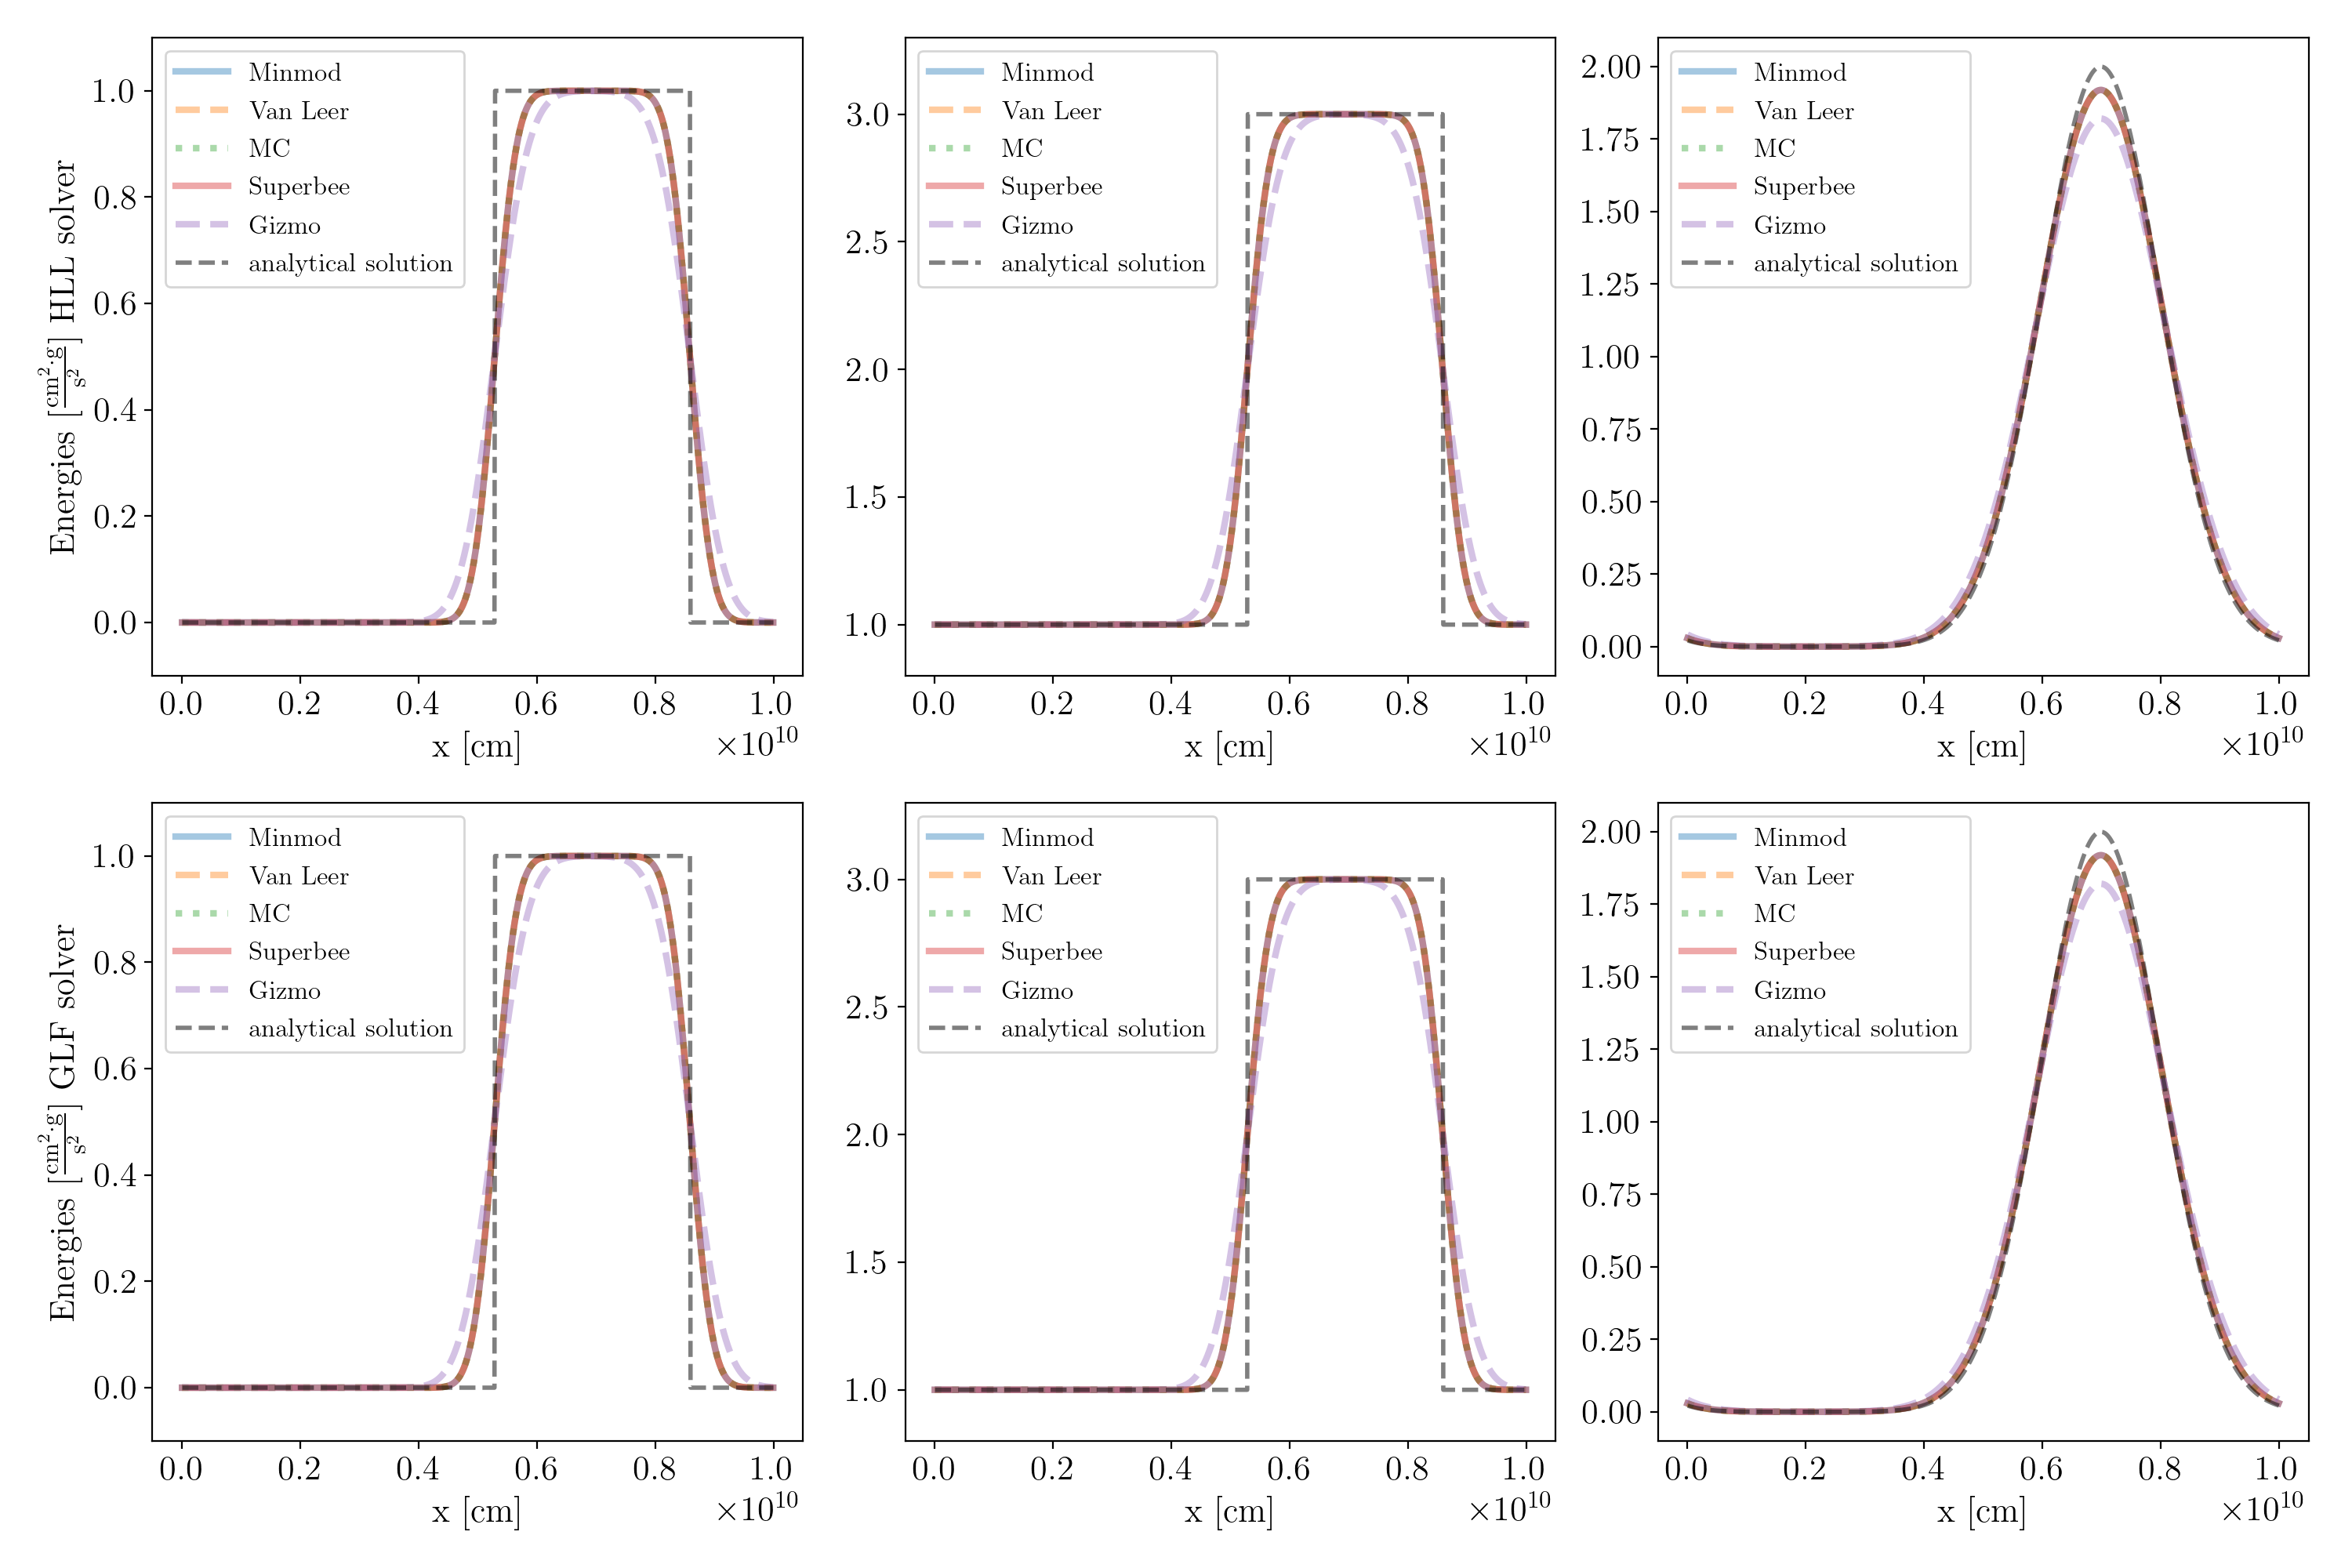
\includegraphics[width=\textwidth]{figures/RHD/Riemann/1D_limiters.png}%
 \caption{
Left: a top hat function; Center: a top hat function where the lower value is nonzero; And Right: a
smooth Gaussian initial energy density being advected using the HLL Riemann solver (top row) and
GLF Riemann solver (bottom row) using various flux limiters.
 }
 \label{fig:rt-riemann-limiter-1D}
\end{figure}




\begin{figure}
 \centering
 \fbox{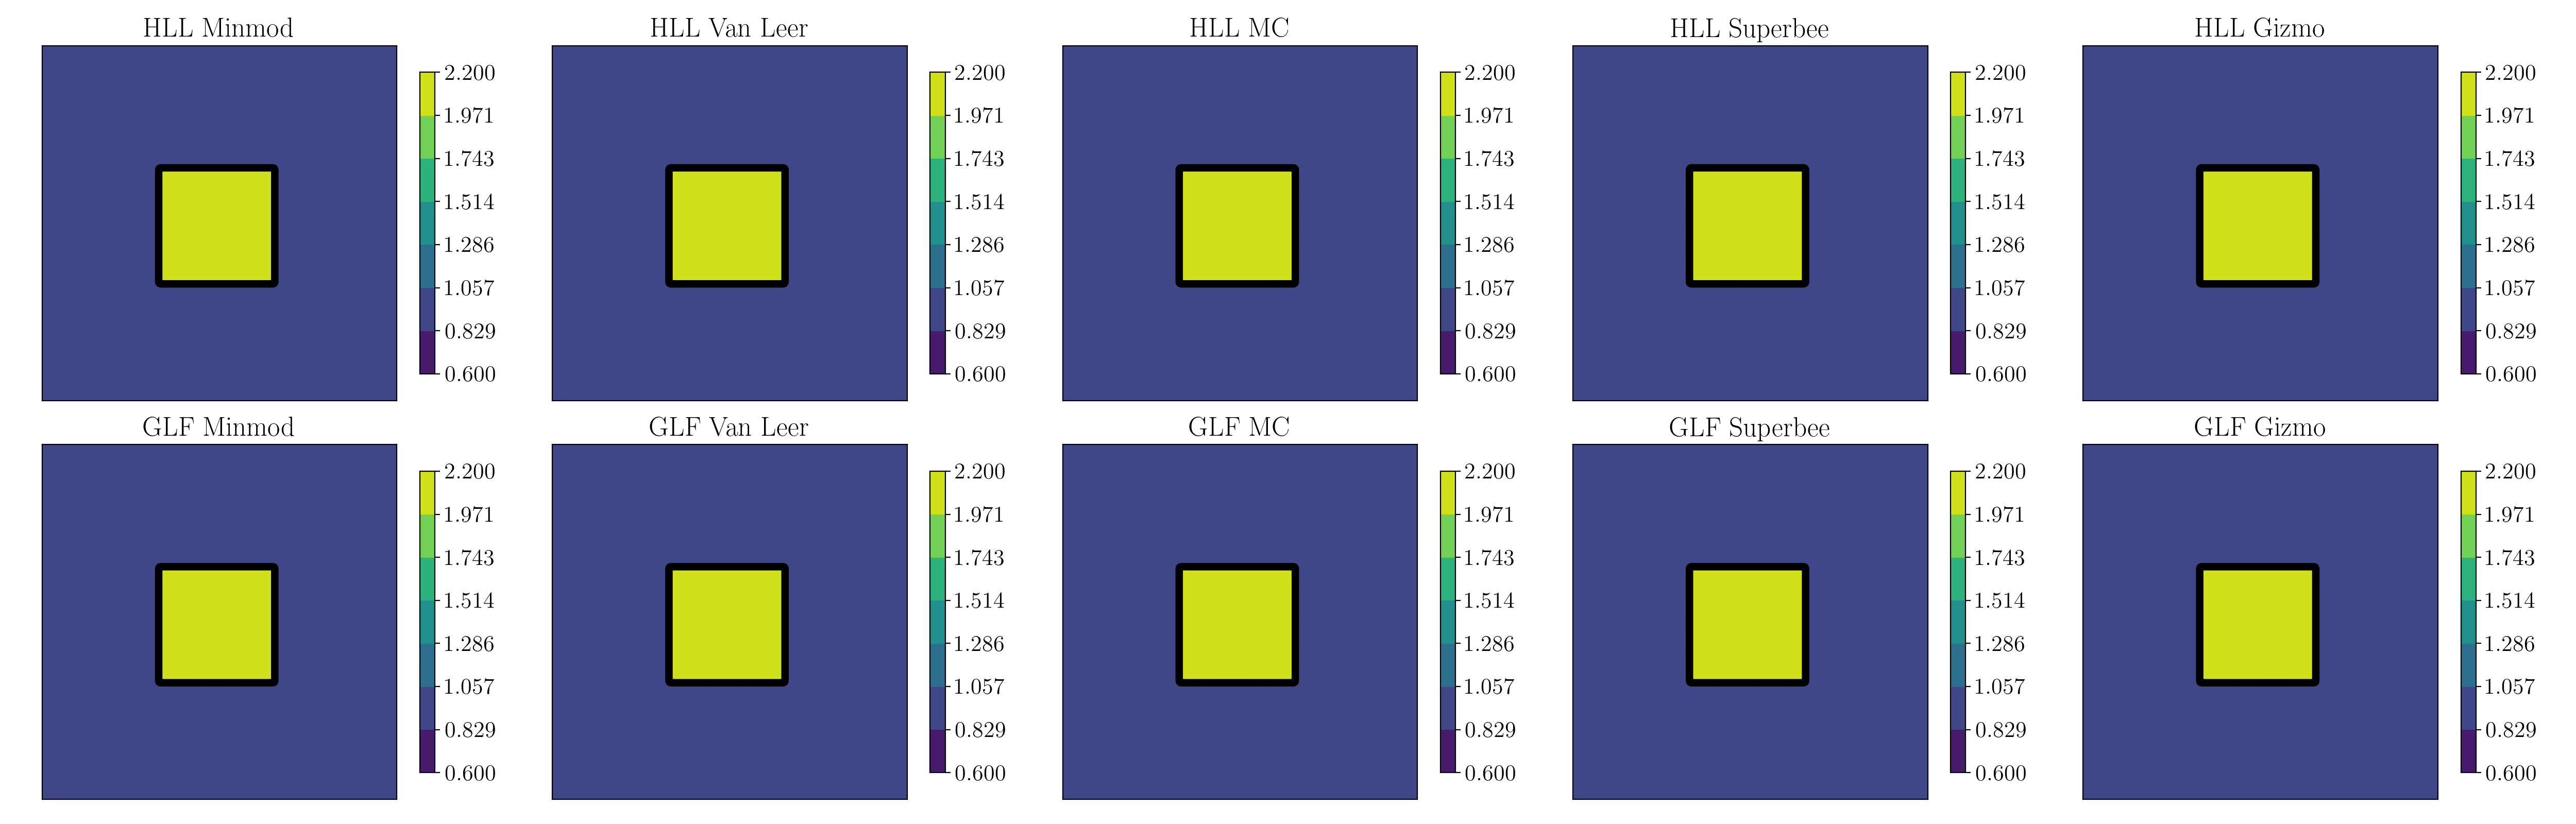
\includegraphics[width=\textwidth]{figures/RHD/Riemann/2D_Group2_init.png}}\\
 \fbox{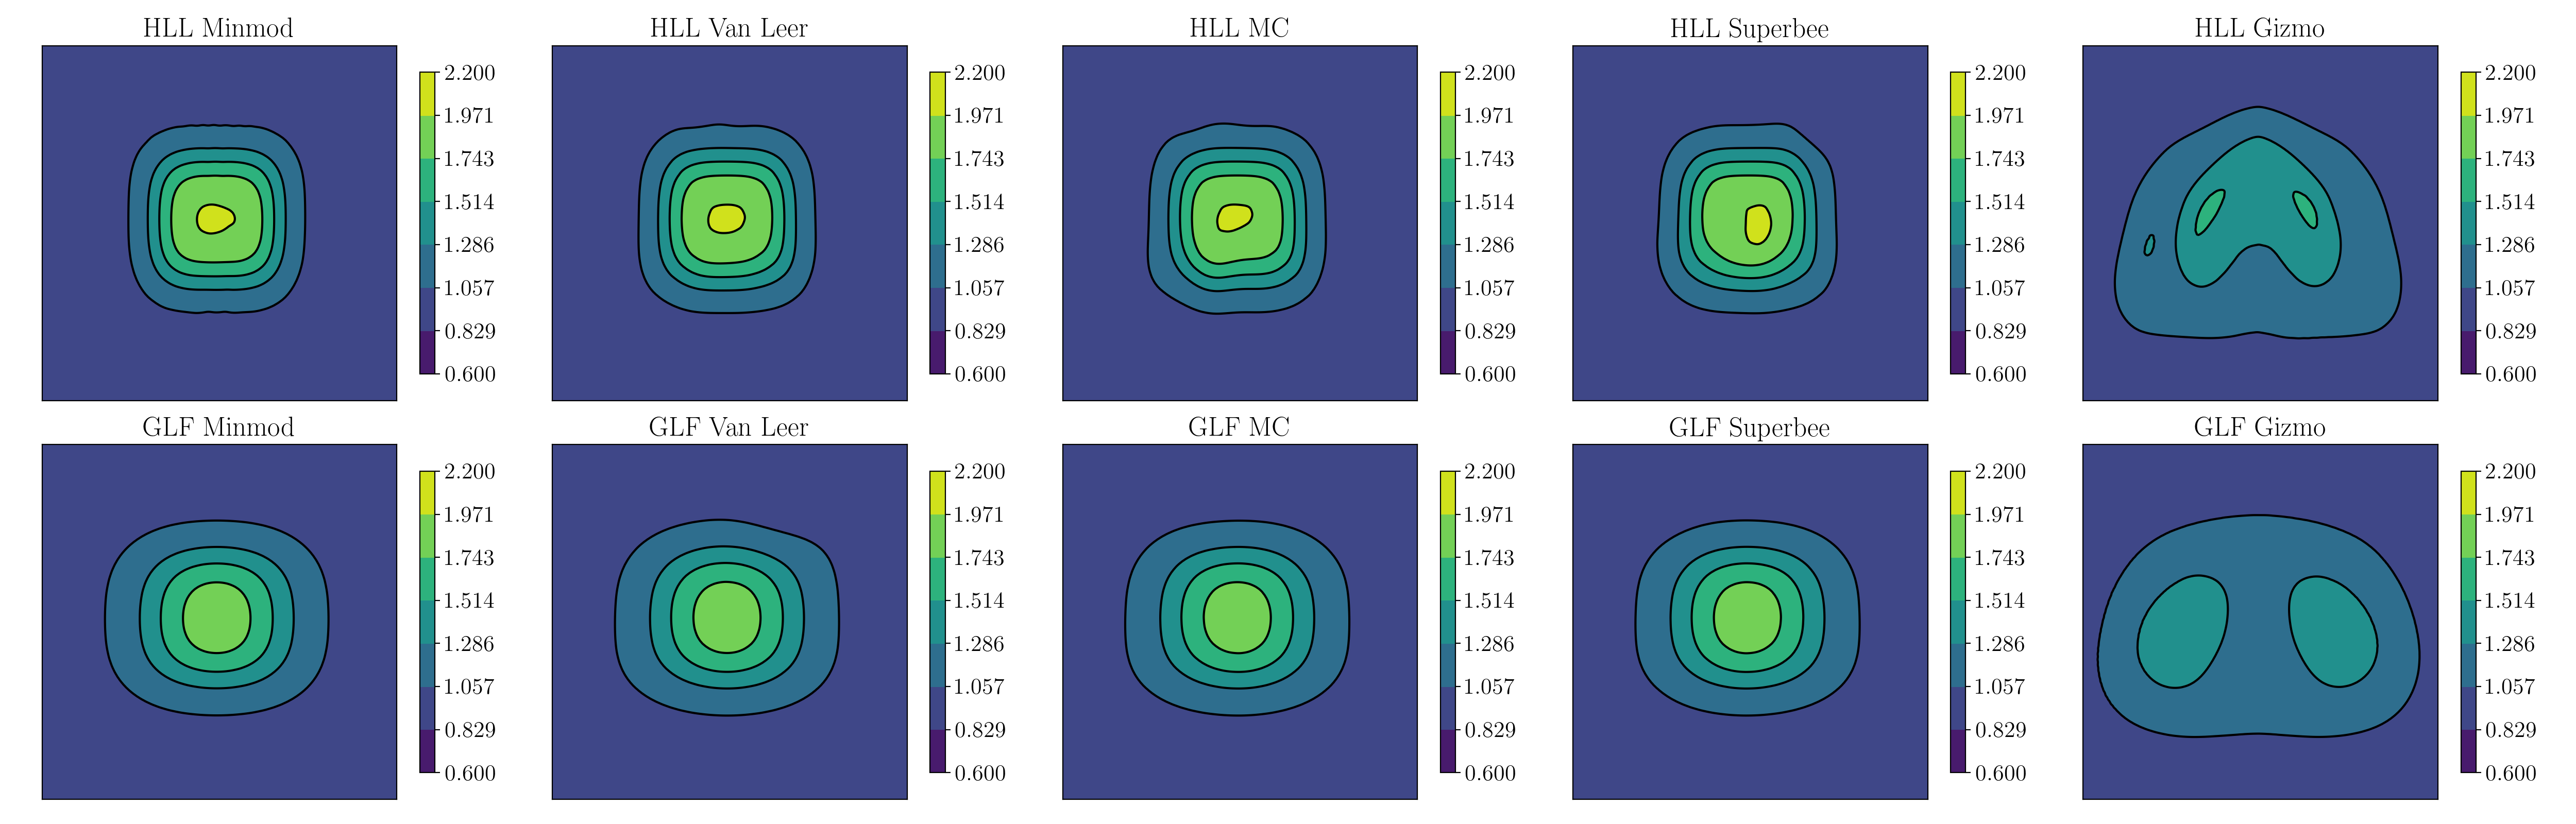
\includegraphics[width=\textwidth]{figures/RHD/Riemann/2D_Group2_end.png}}%
 \caption{
Propagation of a square with non-zero background energy density along the $y$-axis using the GLF
and HLL Riemann solver and various flux limiters. The top figure shows (contours of) the initial
conditions, the bottom figure shows the (contours of the) results after the square propagated a
full box length. The underlying particles were distributed along a uniform grid.
 }
 \label{fig:rt-riemann-limiter-2D-Group2-uniform}
\end{figure}




\begin{figure}
 \centering
 \fbox{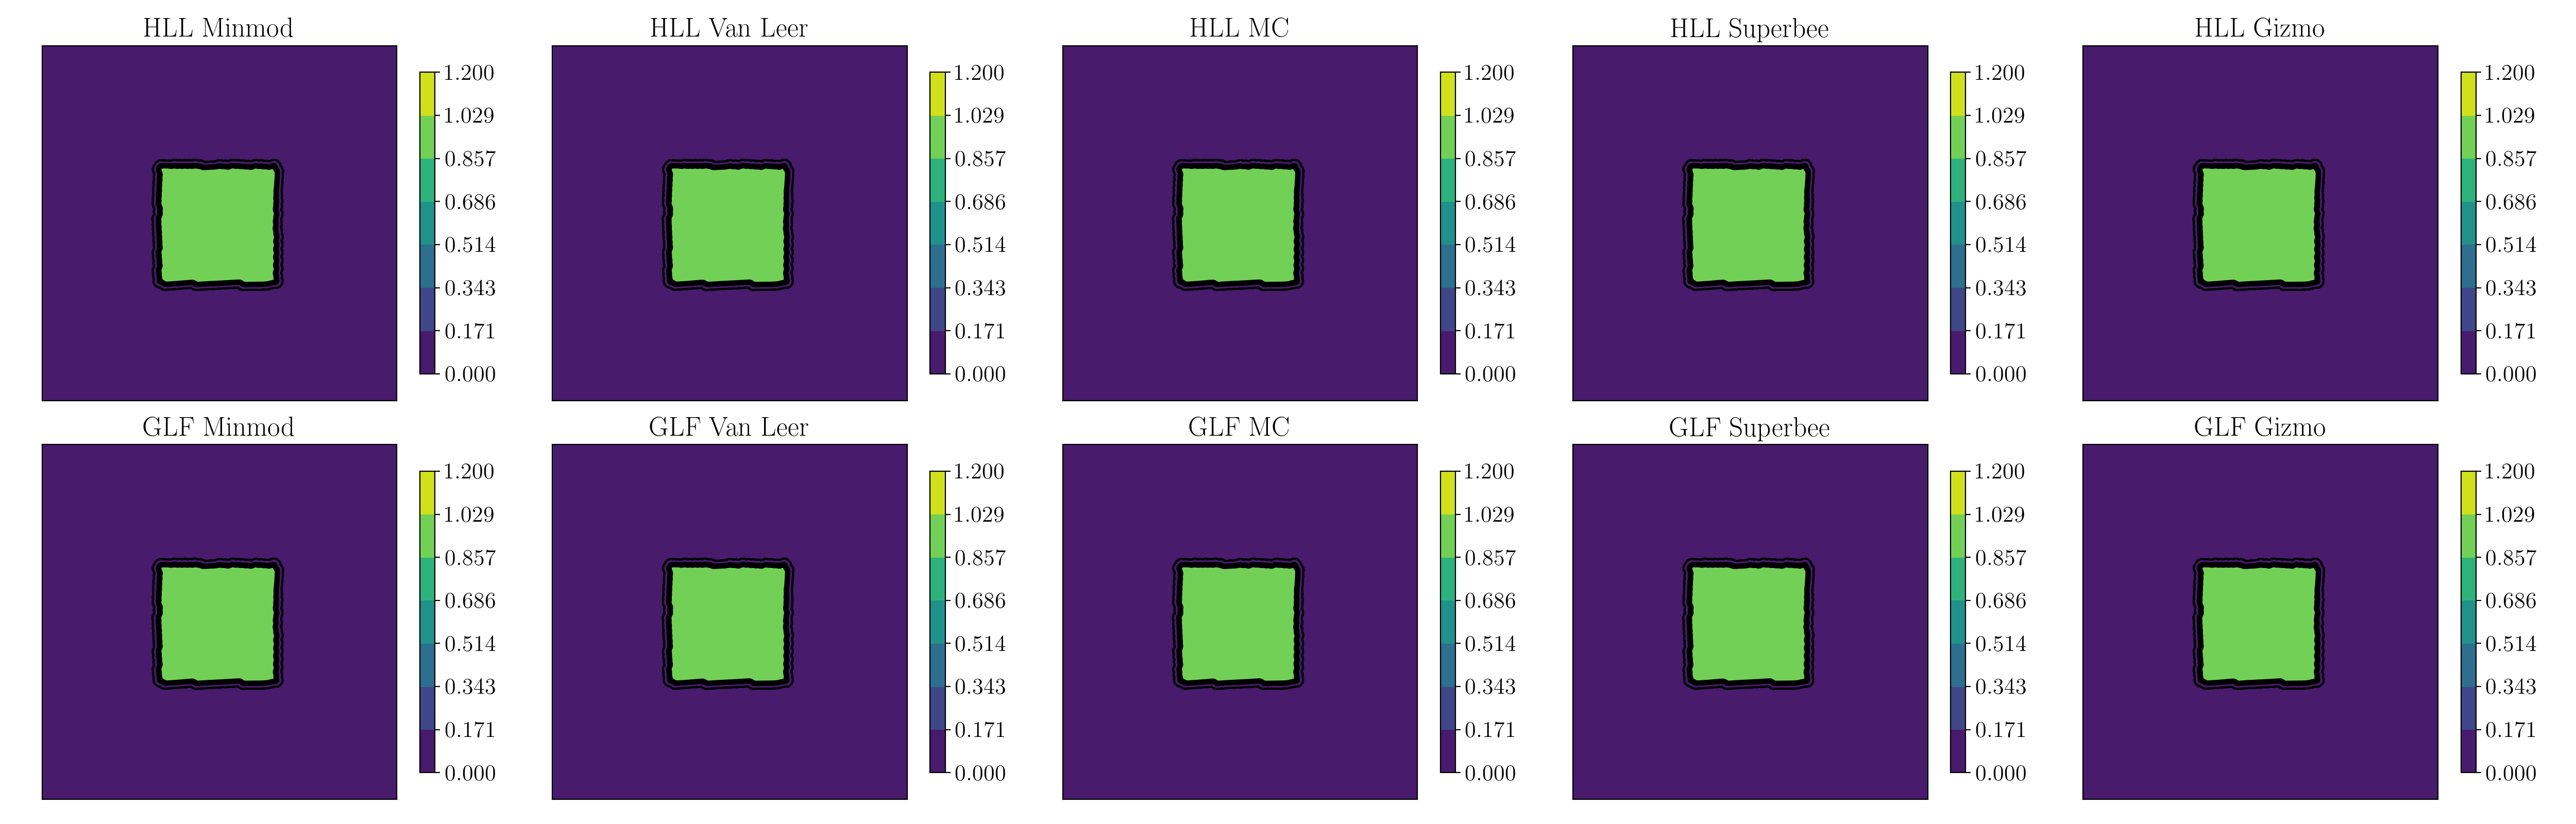
\includegraphics[width=\textwidth]{figures/RHD/Riemann/2D_Group1_init_glass.png}}\\
 \fbox{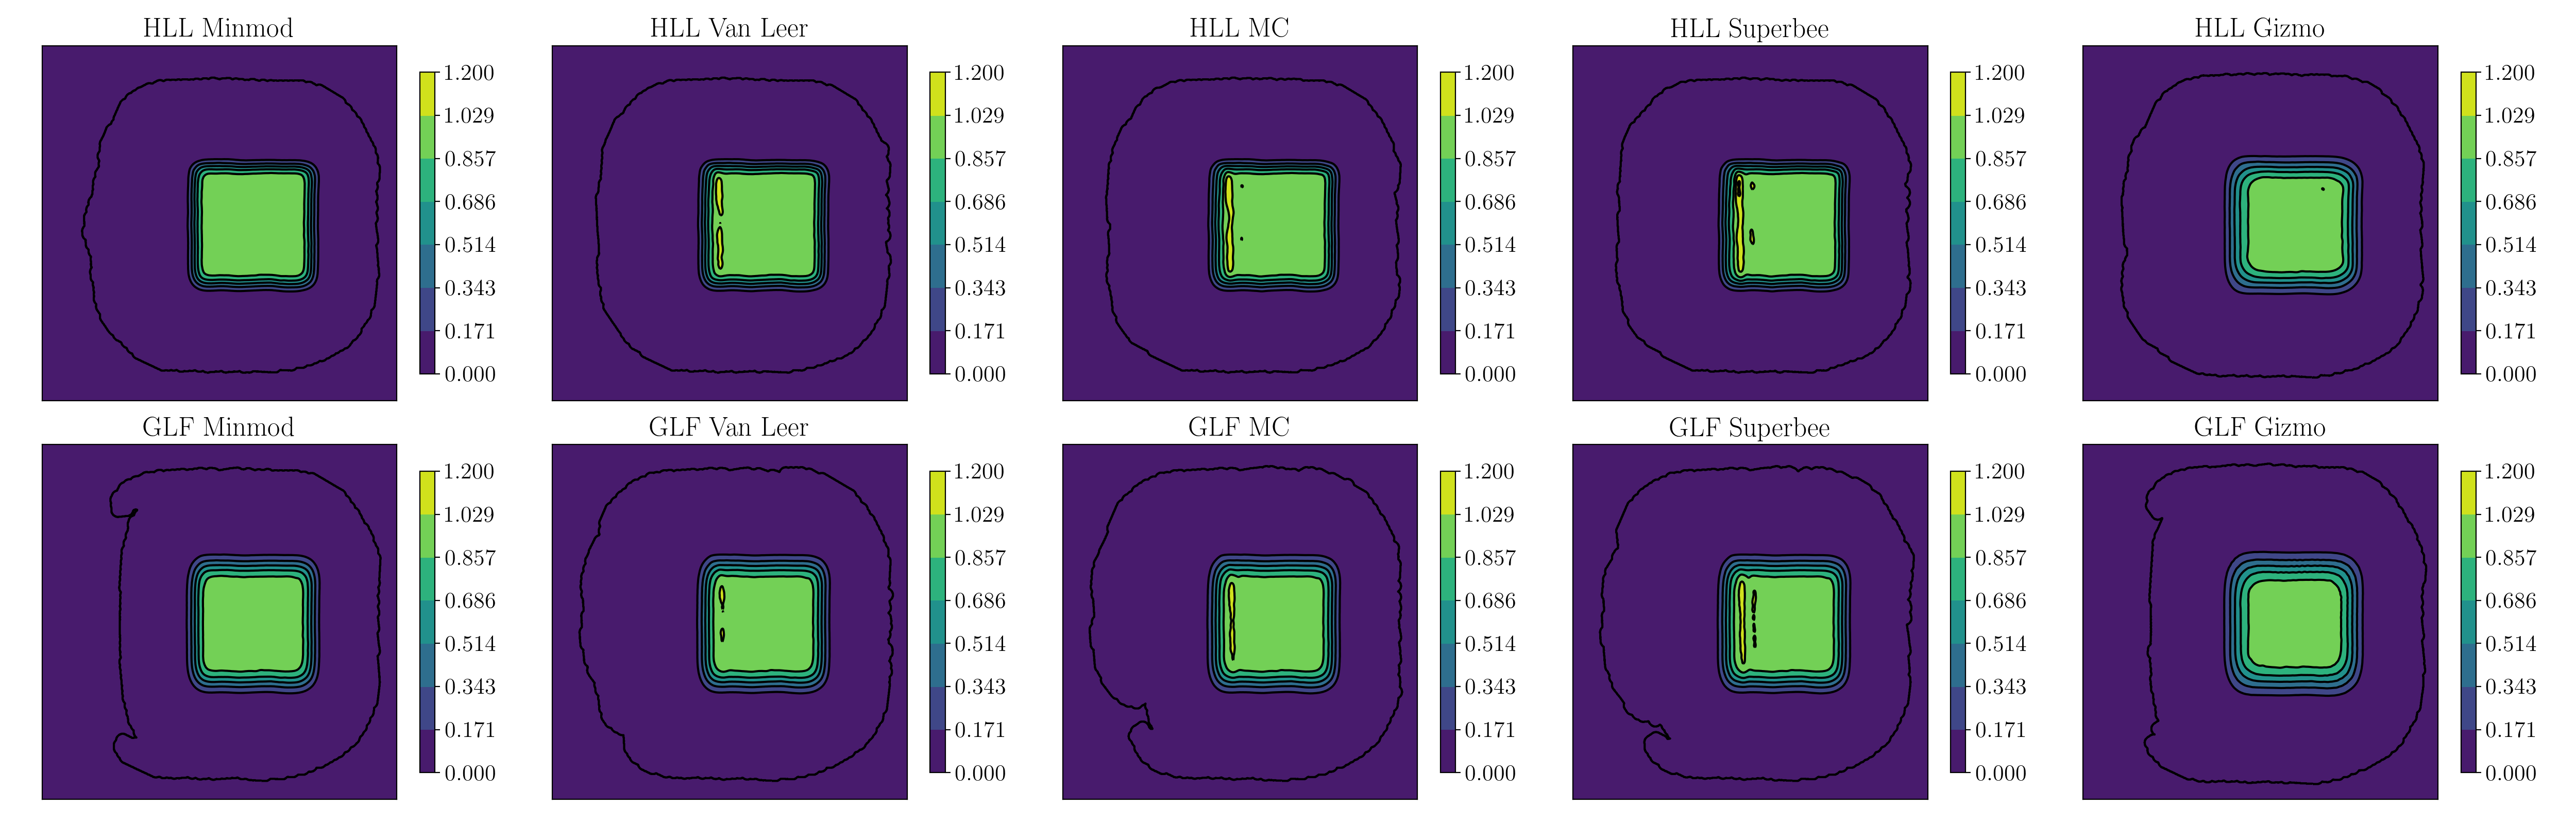
\includegraphics[width=\textwidth]{figures/RHD/Riemann/2D_Group1_step1_glass.png}}\\
 \fbox{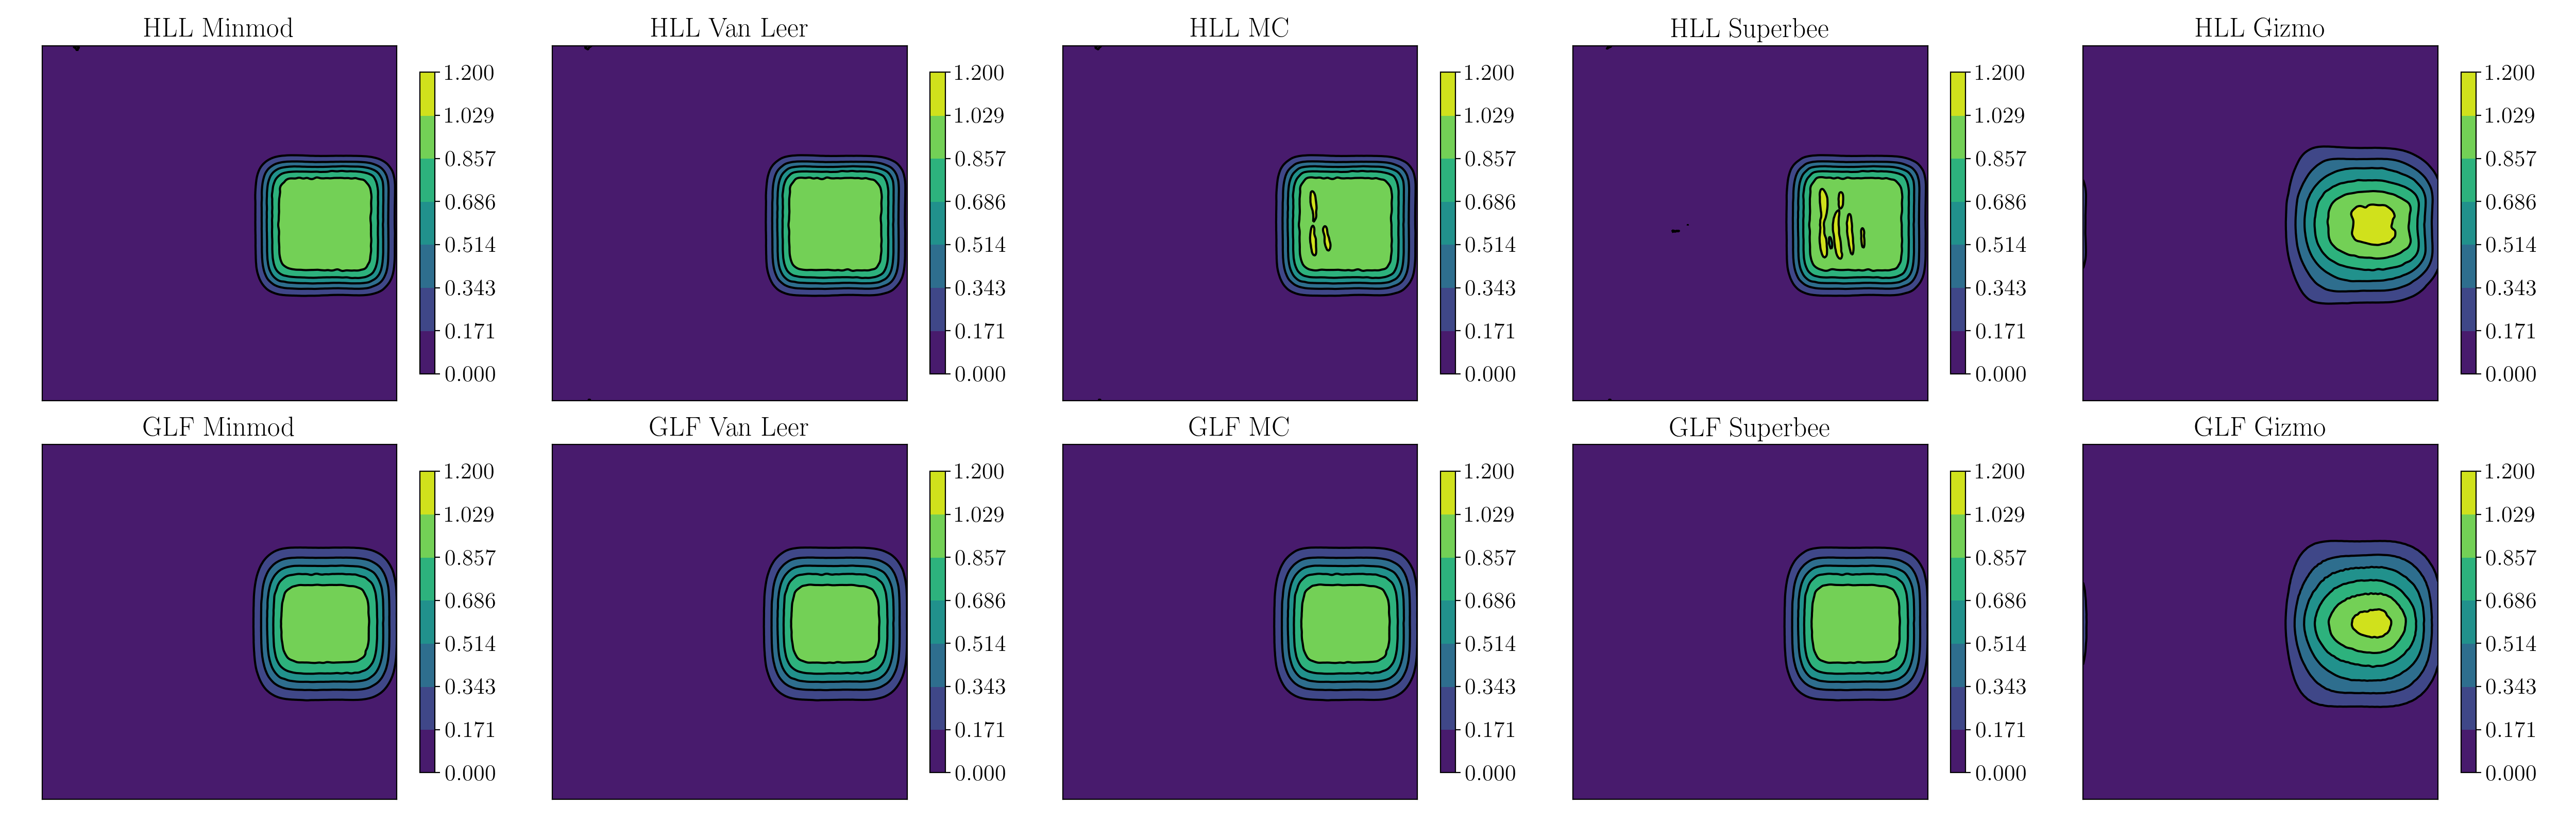
\includegraphics[width=\textwidth]{figures/RHD/Riemann/2D_Group1_step3_glass.png}}\\
 \fbox{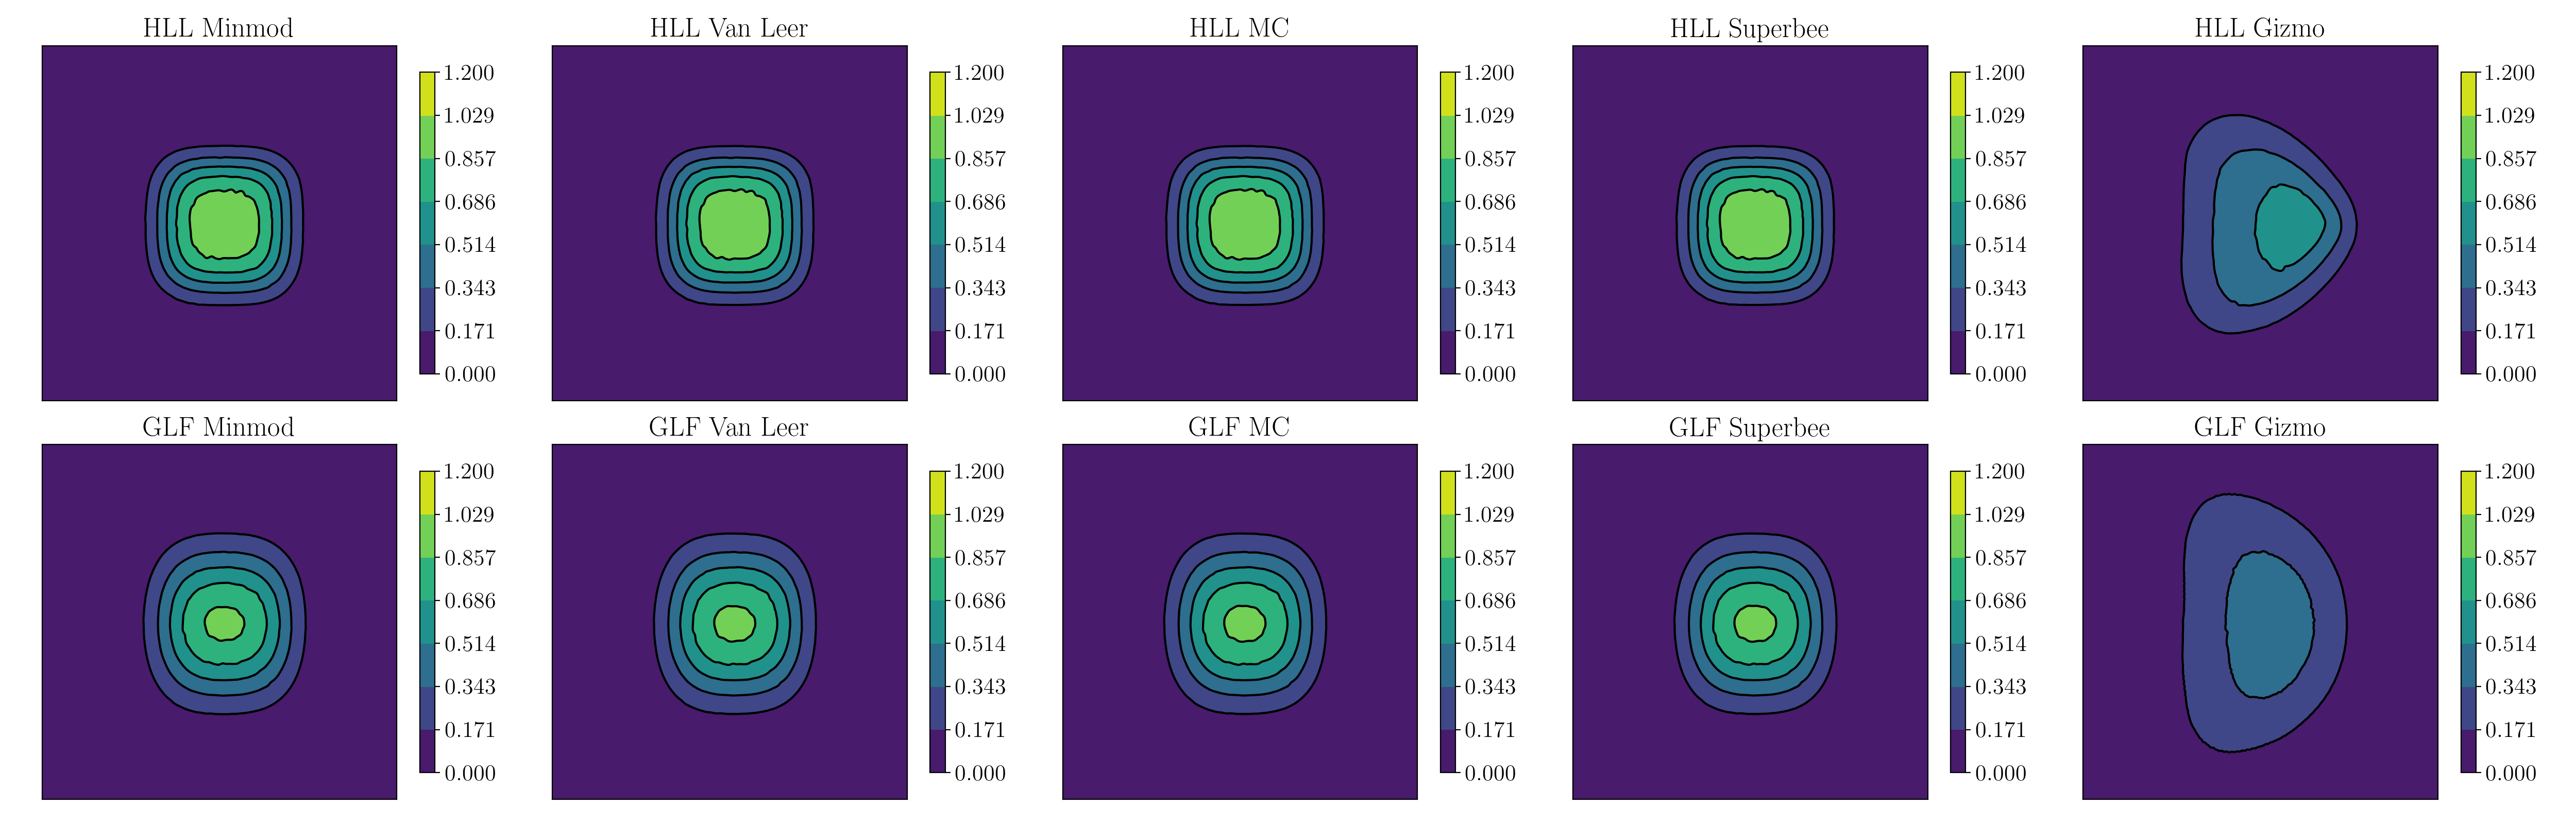
\includegraphics[width=\textwidth]{figures/RHD/Riemann/2D_Group1_end_glass.png}}%
 \caption{
Propagation of a square with non-zero background energy density along the $x$-axis using the GLF
and HLL Riemann solver and various flux limiters. The top figure shows (contours of) the initial
conditions, the bottom figure shows the (contours of the) results after the square propagated a
full box length. The second and third figure show intermediate steps, where the van Leer, MC, and
superbee limiters develop local maxima. The underlying particles were placed in a glass-like
distribution.
 }
 \label{fig:rt-riemann-limiter-2D-Group1-glass}
\end{figure}



\begin{figure}
 \centering
 \fbox{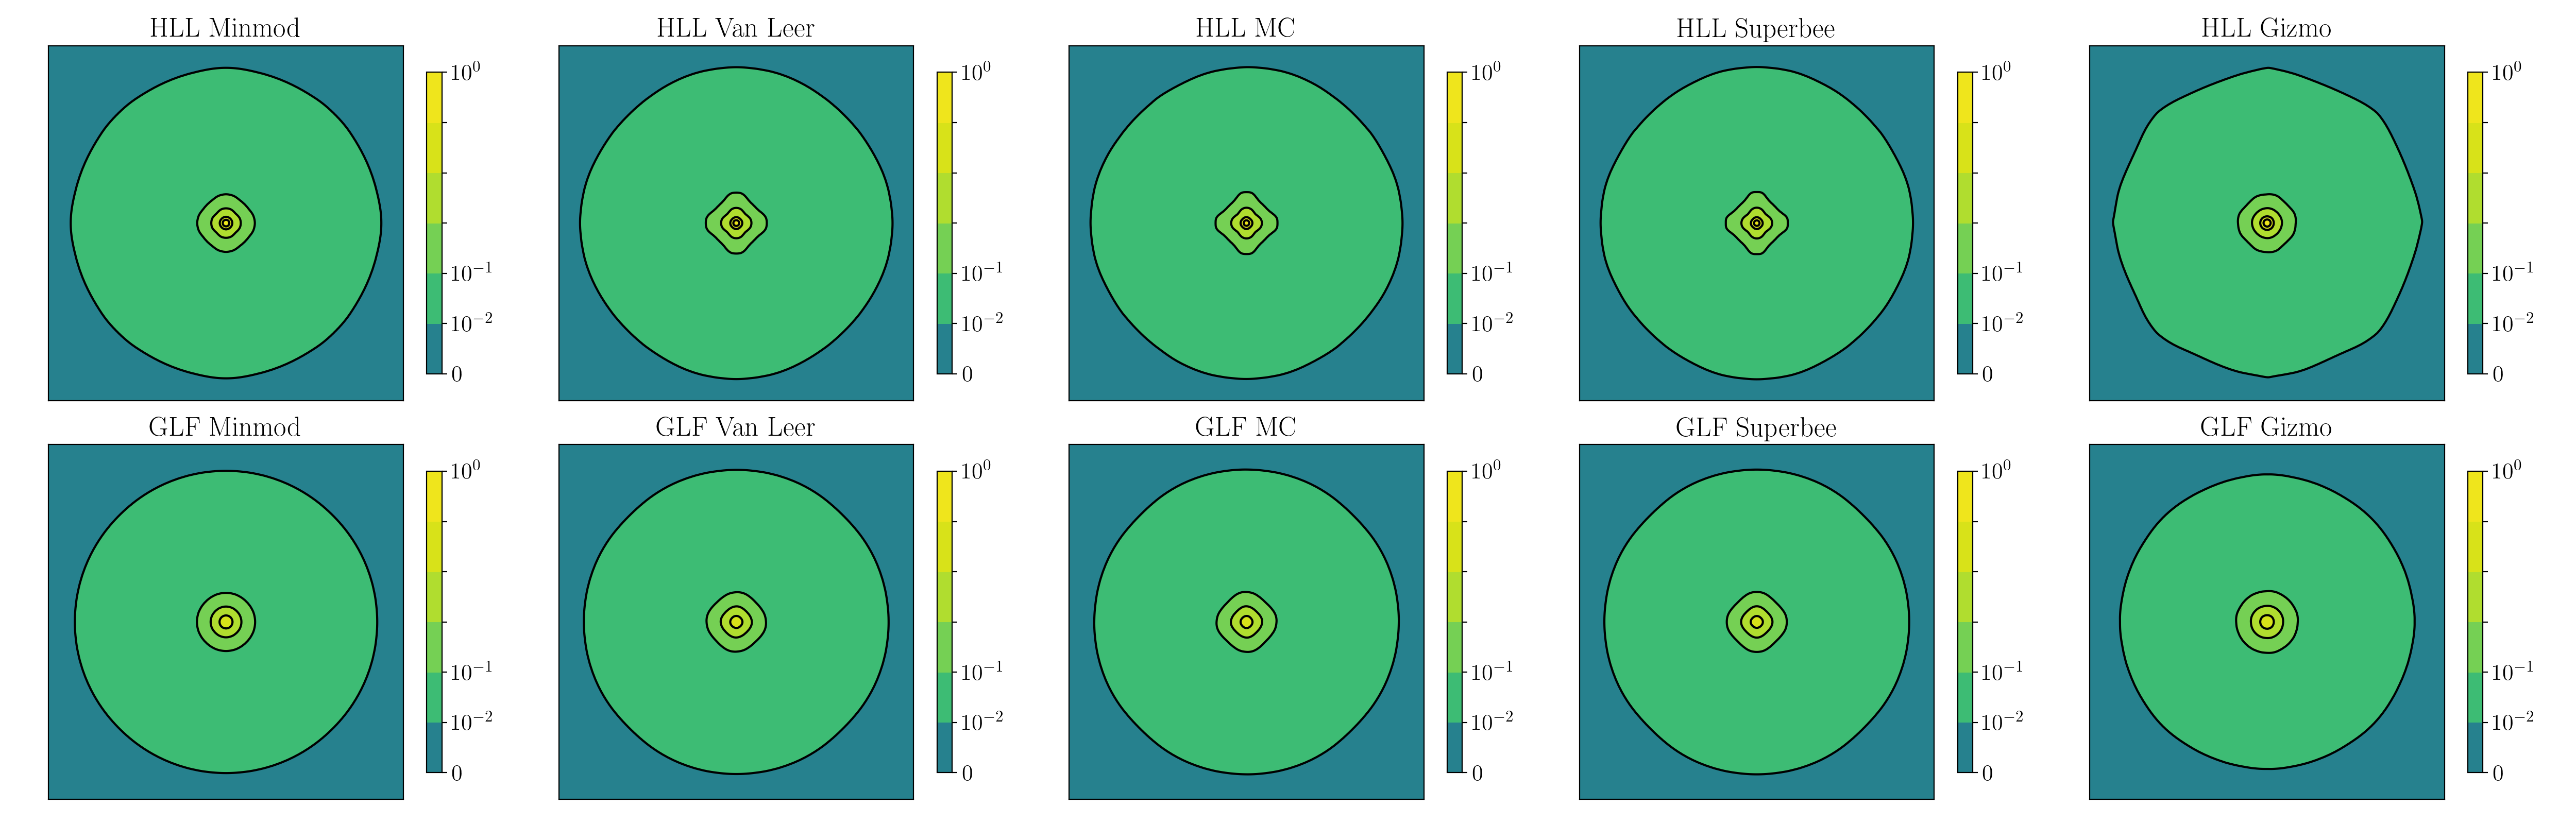
\includegraphics[width=\textwidth]{figures/RHD/Riemann/injection_2D_uniform.png}}\\
 \fbox{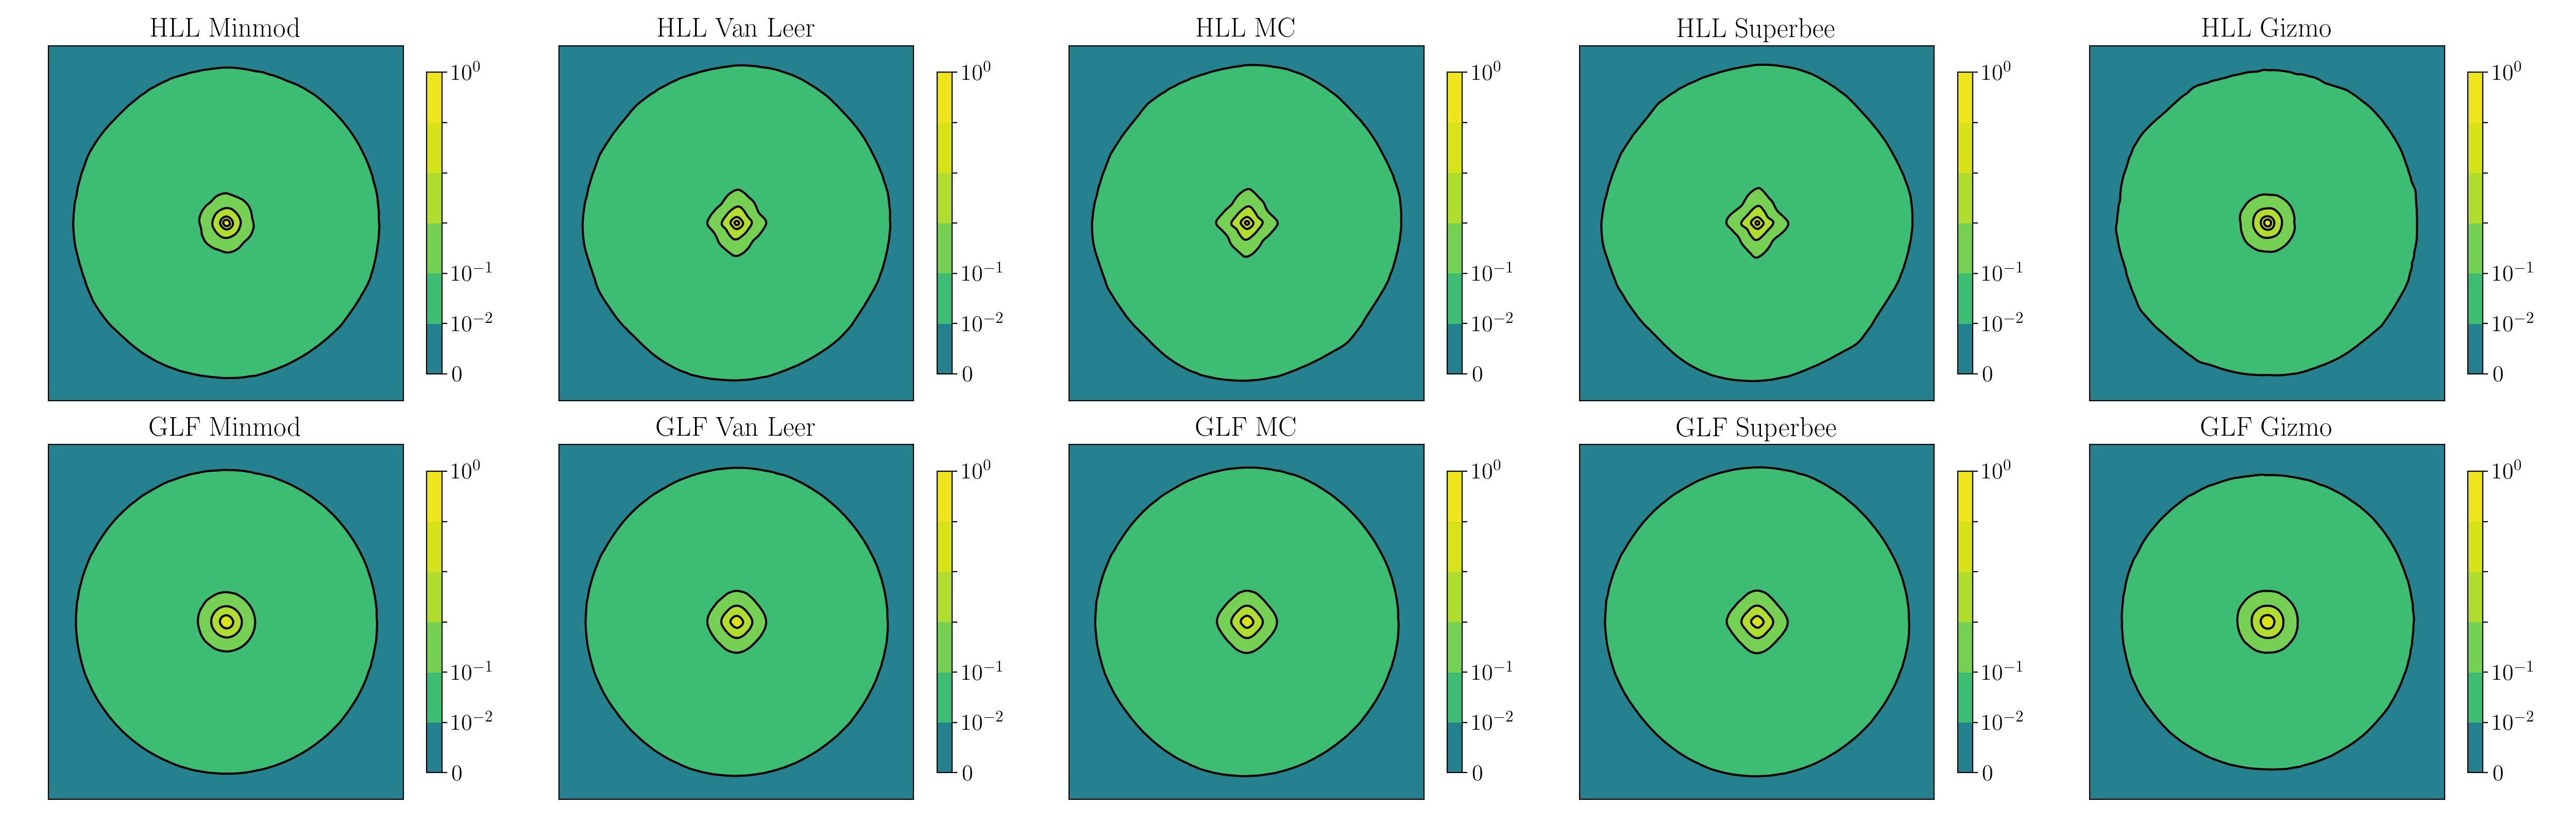
\includegraphics[width=\textwidth]{figures/RHD/Riemann/injection_2D_glass.png}}%
 \caption{
Isotropic injection of radiation energy density from a central source evolved over time using
various limiters and both Riemann solvers. The top figure shows the results using a regular
particle distribution, the bottom figure shows the solution on a glass-like particle configuration.
 }
 \label{fig:rt-riemann-limiter-2D-injection}
\end{figure}









In this section, results of simple photon transport tests using varying Riemann solvers and flux
limiters are shown. The experiments are set up such that the radiation is only advected, and
doesn't interact with the gas at all.

To test the photon transport in 1D, the following initial conditions are set up: (i) a top hat
function, (ii) a top hat function where the lower value is nonzero, and (iii) a smooth Gaussian. The
second top hat function with a nonzero lower value is used to test for cases where the solution
develops oscillations that would predict negative energy densities if the lower limit were zero. In
such cases \GEARRT would correct them, i.e. set the energy density to zero. By having a nonzero
lower value, these instabilities will show up.

Figure~\ref{fig:rt-riemann-limiter-1D} shows the results using various limiters for both the HLL and GLF Riemann solvers (see Section \ref{chap:riemann-rt} for details). The results are virtually
indistinguishable, with the only exception of the ``Gizmo'' limiter
(eqns.~\ref{eq:face-limiter-first}-\ref{eq:face-limiter-last}) being somewhat more diffusive.

Figure~\ref{fig:rt-riemann-limiter-2D-Group2-uniform} shows the propagation of a square along the
$y$-axis with a non-zero background energy density using the two Riemann solvers and various
limiters. In general, the HLL solver indeed delivers less diffusive results, as it promised to do.
The ``Gizmo'' flux limiter however delivers much too diffusive results, despite being a more
sophisticated model. Due to its additional expense yet worse results, it shouldn't be used for the
purposes radiative transfer.


Figure~\ref{fig:rt-riemann-limiter-2D-Group2-uniform} used uniformly distributed particles as the
underlying configuration. Using a glass-like file instead leads to similar results, which are shown
in Figure~\ref{fig:rt-riemann-limiter-2D-Group1-glass} for a square being advected along the
$x$-axis. Additionally, in the test shown in Figure~\ref{fig:rt-riemann-limiter-2D-Group1-glass}, a
zero background energy density is assumed. Looking at intermediate steps, i.e. before the square
transverses a full box length, some local maxima develop for the van Leer, superbee and MC flux
limiters, indicating that they do not make this method truly TVD, and as such are not
unconditionally stable. Hence I advise strongly against the use of them, and to opt for the minmod
limiter instead.\footnote{
It should be noted that due to these findings, the choice of the limiter is not given as a free
parameter to users, as it could lead to unstable results and crashes. The minmod limiter is taken
by default. However, changing the flux limiter is a simple exercise, and the functions of the other
limiters described in this work remain in the source code of \GEARRT. The choice of the Riemann
solver remains a free compile time parameter.
}


Lastly, Figure~\ref{fig:rt-riemann-limiter-2D-injection} shows the results of radiation energy
density being injected isotropically from a single central source and evolved over time using
various flux limiters and both Riemann solvers, using both a glass-like and a uniform underlying
particle configuration. In nearly all cases small deformities, i.e. deviations from perfect circles,
can be seen close to the source, but they even out with increasing distance. Notably the HLL Riemann
solver doesn't show deformities nowhere nearly as strong as reported in \citet{ramses-rt13} even
when using the uniform particle configuration. The reason is that contrary to grid codes, which in
2D would only interact any cell with its eight adjacent neighbors, \GEARRT uses more neighboring
particles ($\sim 15$ in this example for $\eta_{res} = 1.2348$ and the cubic spline kernel), leading
to the improved isotropy of the solution. The use of more neighbors compared to grid codes was
indeed a motivation to make use of the HLL solver, which should perform better in terms of creating
shadows compared to the GLF solver, while the particle nature of \GEARRT and the use of more
neighbors can sidestep the anisotropies seen in grid codes.




%========================================================
\subsection{Order of Accuracy}
%========================================================


\begin{figure}
    \centering
    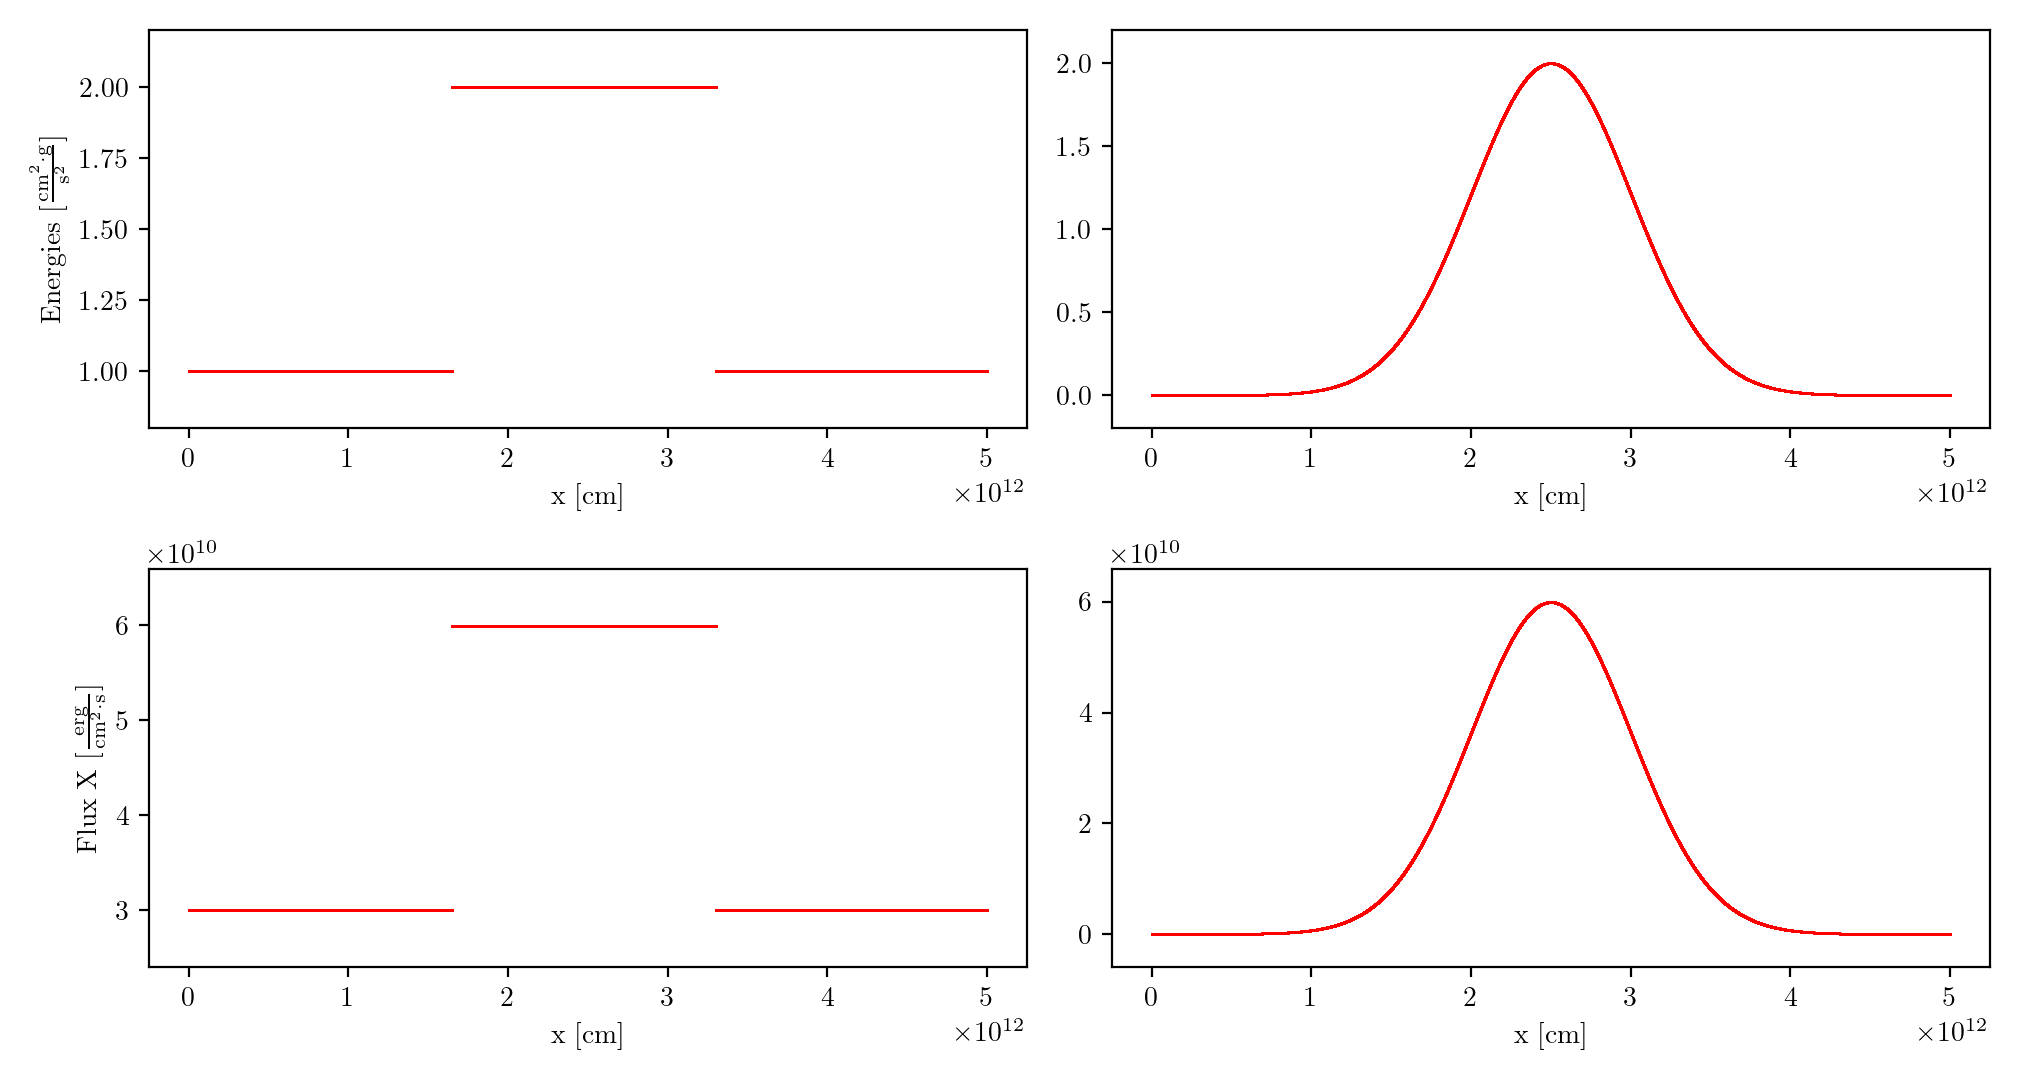
\includegraphics[width=\textwidth]{figures/RHD/accuracy/IC.png}%
    \caption{Initial conditions for the order of accuracy test: A smooth Gaussian and a top hat
function.}
    \label{fig:result-convergence-IC}
\end{figure}


\begin{figure}
    \centering
    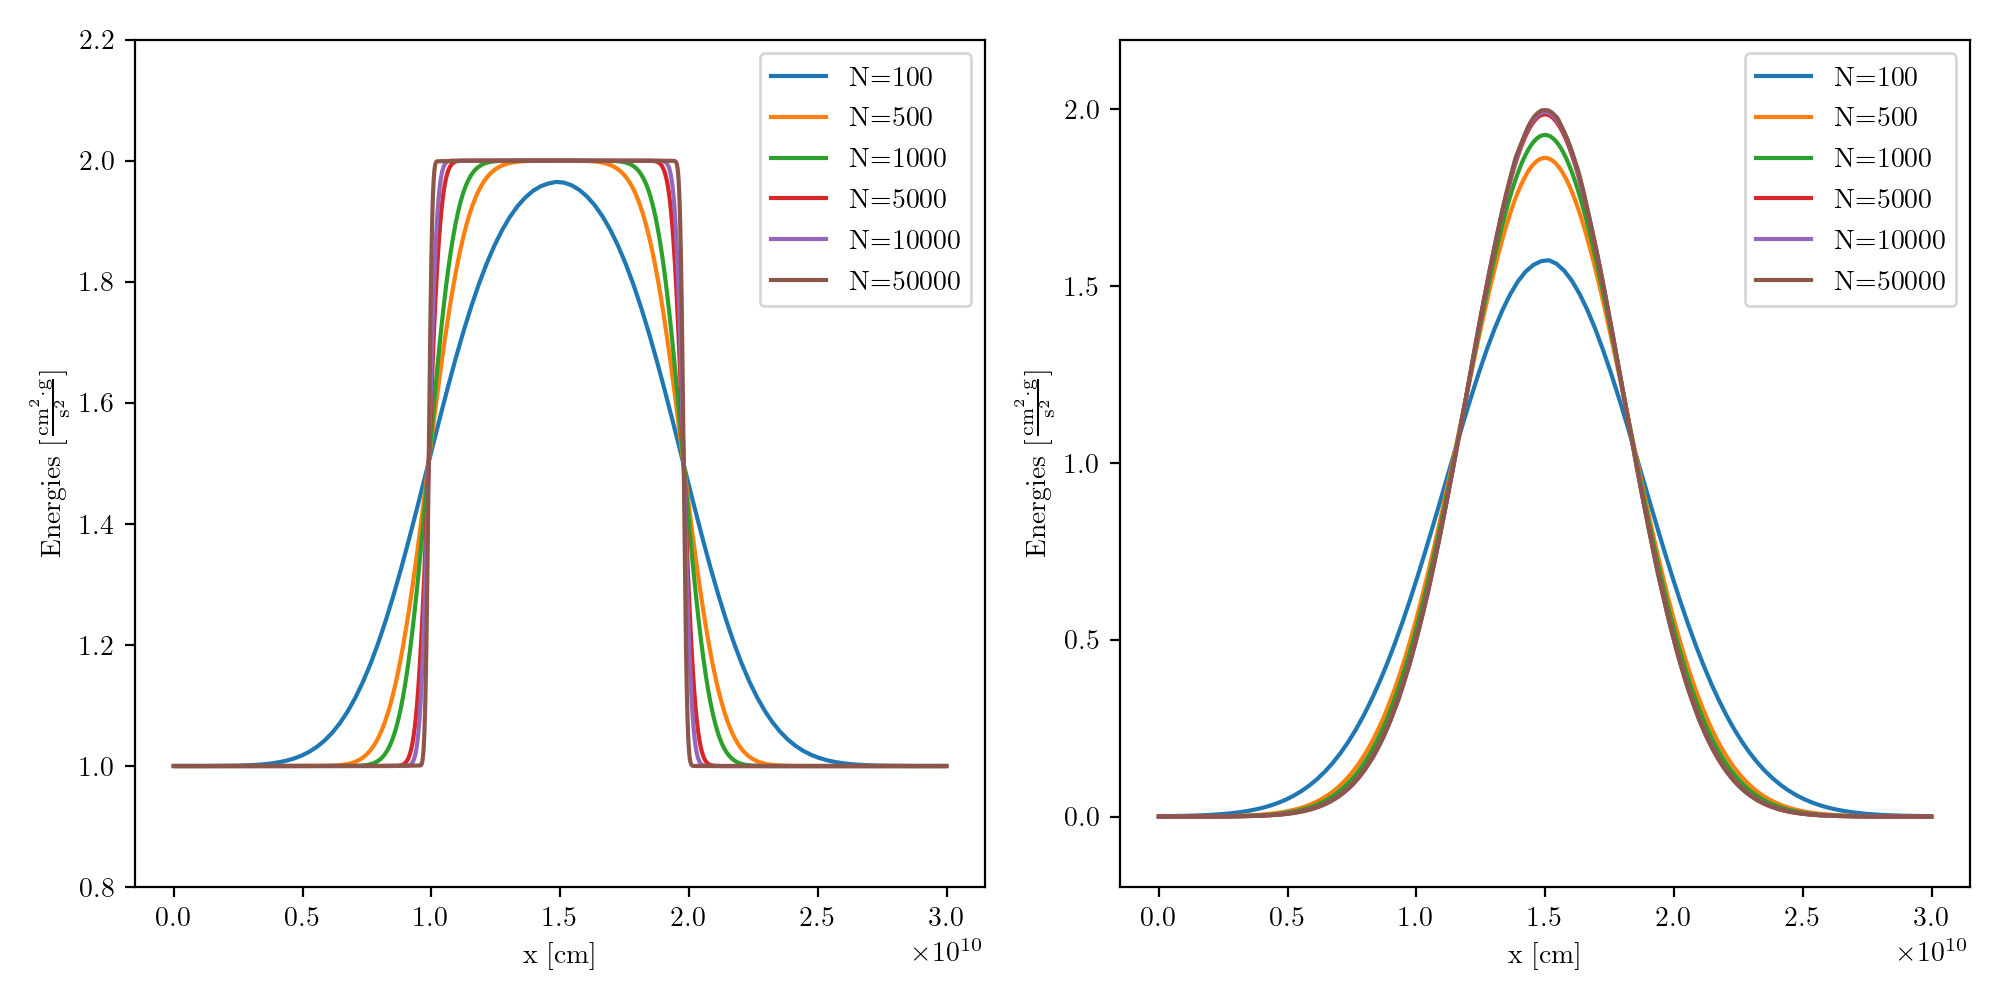
\includegraphics[width=\textwidth]{figures/RHD/accuracy/results-fixed-boxsize.png}%
    \caption{
The results of the order of accuracy test at $t = 1$s for varying number of particles $N$ used, as
indicated in the legend, for a fixed box size $L = c \times 1$s.
    }
    \label{fig:convergence-energy-fixed-boxsize}
\end{figure}


\begin{figure}
    \centering
    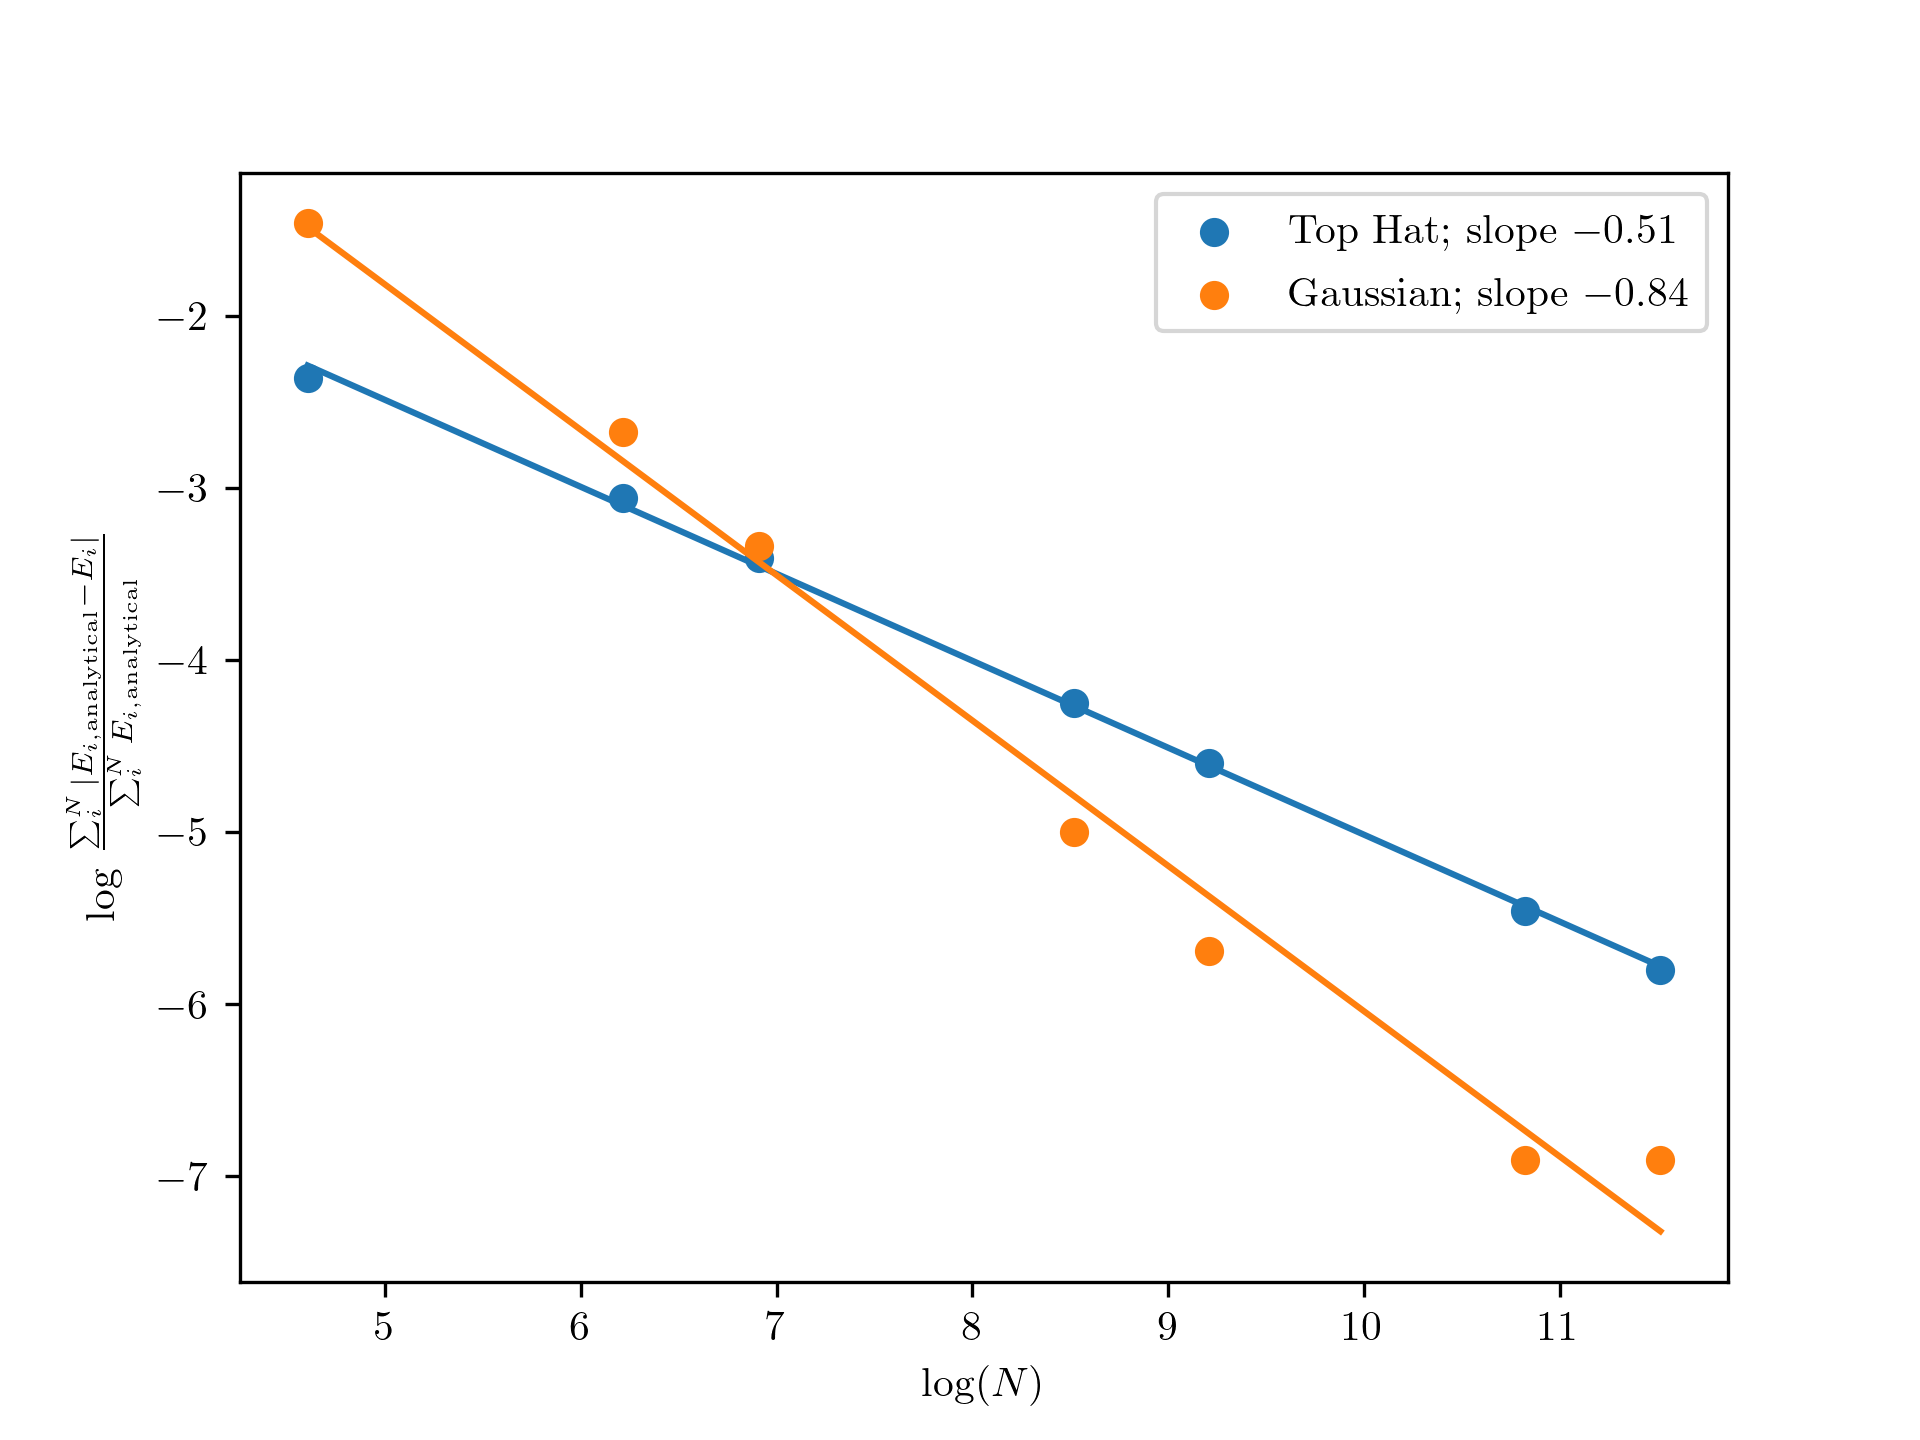
\includegraphics[width=.75\textwidth]{figures/RHD/accuracy/convergence-fixed-boxsize.png}%
    \caption{
Order of accuracy for \GEARRT with increasing particle numbers $N$, as indicated in the legend,
for simulations using the identical box size length $L = c \times 1$s and end time $t = 1$s.
According to expectations for a second order accurate scheme, the photon transport for the smooth
Gaussian converges with a power of nearly $-1$, while the exponent is reduced to $-1/2$ for the top
hat function due to its discontinuities. The slopes are best fits to the measurements (circles).
Note that the slopes aren't $-2$ and $-1$, respectively, because in this setup, the simulations
with
higher particle numbers $N$ also need to perform more time steps to reach the same end time $t$,
and thus accumulating more one step errors over the course of the run (compare with
Section~\ref{chap:numerical_diffusion}). The expected slopes of $-2$ and $-1$ are achieved when
keeping the number of time steps fixed as well, which is shown in
Figure~\ref{fig:result-convergence}.
    }
    \label{fig:result-convergence-fixed-boxsize}
\end{figure}



\begin{figure}
    \centering
    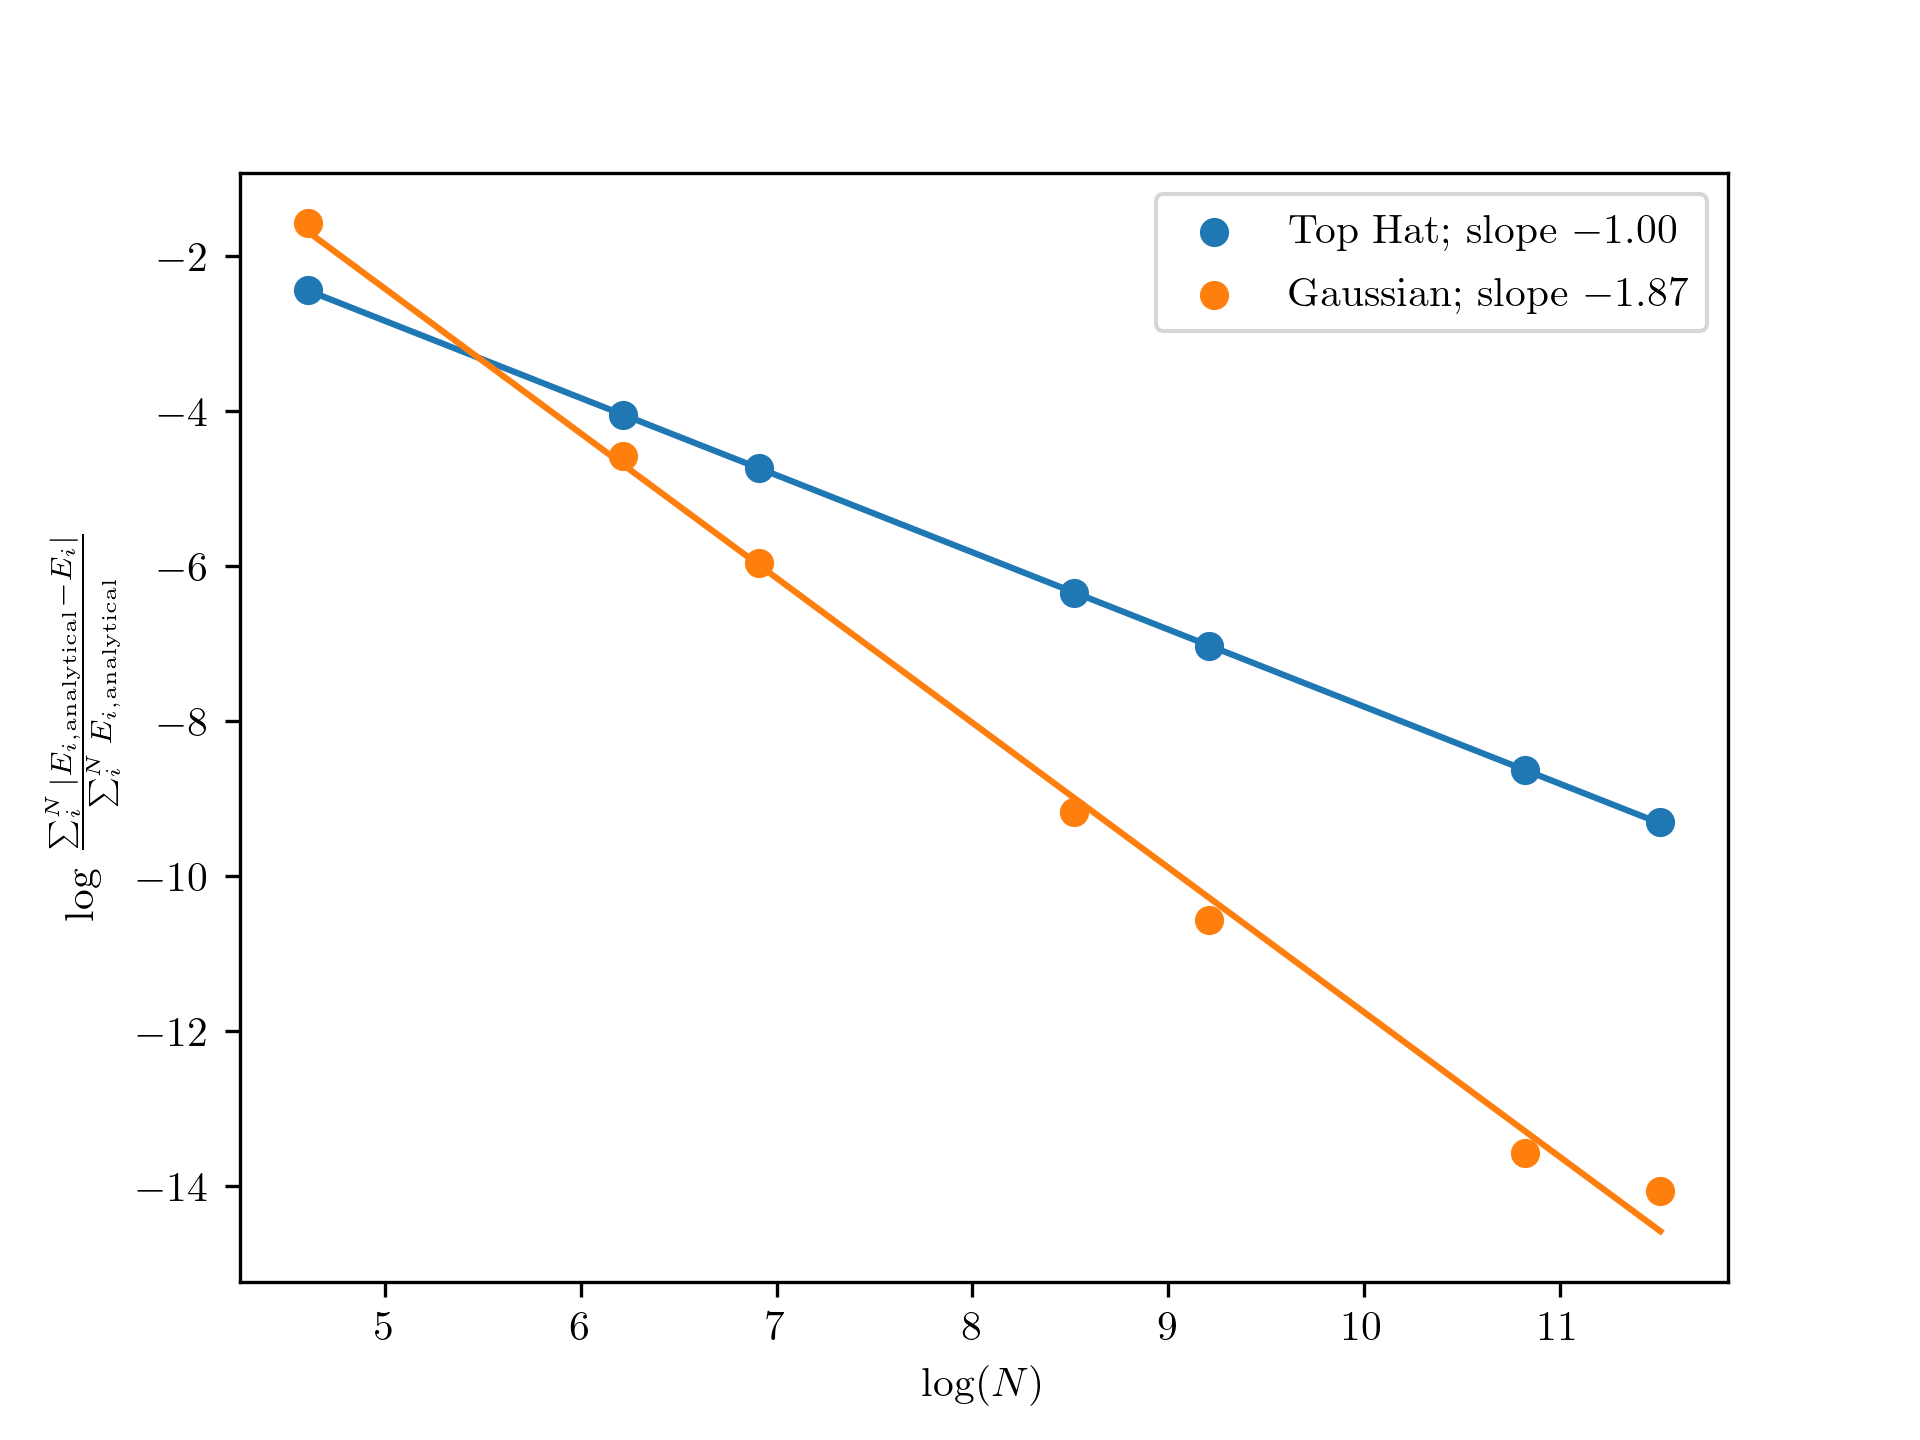
\includegraphics[width=.75\textwidth]{figures/RHD/accuracy/convergence.png}%
    \caption{
Order of accuracy for \GEARRT with increasing particle numbers. According to expectations for a
second order accurate scheme, the photon transport for the smooth Gaussian converges with a power
of
nearly $-2$, while the exponent is reduced to $-1$ for the top hat function due to its
discontinuities. The slopes are best fits to the measurements (circles).
    }
    \label{fig:result-convergence}
\end{figure}




To demonstrate the order of accuracy of radiation transport solved by the finite volume particle
method, the same experiments as for the finite volume methods in Part~\ref{part:finite-volume} are
conducted. Two test cases are set up: One where the initial conditions are a top hat function for
the photon energy density, and one where the initial conditions are a smooth Gaussian. The photon
fluxes are assigned assuming the free streaming limit $\Fbf = c E$, such that the analytical
solution consists of the equivalent of linear advection of the initial functions to the right. The
gas isn't allowed to interact with the radiation. The initial setup is shown in
Figure~\ref{fig:result-convergence-IC}. The experiments are conducted in one dimension, and with an
increasing number of particles, as indicated in the plots depicting the results.

A first test, intended to facilitate visual inspection of the results alongside the order of
accuracy of the method, keeps the simulation box size and end time constant, while varying the
number of particles, and hence the mean inter-particle distance. The simulation box size is set up
to be $L = c \times 1$s, and the simulation runs until $t = 1$s is reached.
%
Figure~\ref{fig:convergence-energy-fixed-boxsize} shows the resulting energy densities at $t = 1$s.
In agreement with the findings in Section~\ref{chap:numerical_diffusion}, the results improve, i.e.
are less diffusive and maintain the original shapes better, with increasing particle numbers used.
The resulting order of accuracy along with a fit for the slopes are shown in
Figure~\ref{fig:result-convergence-fixed-boxsize} of this setup, where the errors in each simulation
is estimated as

\begin{align}
 Err = \frac{\sum_{i=1}^N |E_{i, \text{analytical}} - E_i|}{\sum_{i=1}^N E_{i, \text{analytical}}}
\ .
\end{align}

Here $i$ denotes the index of particles, and $N$ is the total number of particles. The slopes don't
reach the optimal values of $-2$ for the smooth Gaussian and $-1$ for the discontinuous top hat
function, respectively, because the runs with more particles also require more time steps to reach
the same end time, thus accumulating more one step errors (compare with
Section~\ref{chap:numerical_diffusion}). Comparing the order of accuracy after a fixed number of
time steps for each number of particles $N$ used leads to the anticipated slopes of (nearly) $-2$
and $-1$, respectively, which is shown in Figure~\ref{fig:result-convergence}.











%========================================================
\subsection{Testing the Drift Corrections}\label{chap:validation-drift-corrections}
%========================================================


\begin{figure}
 \centering
 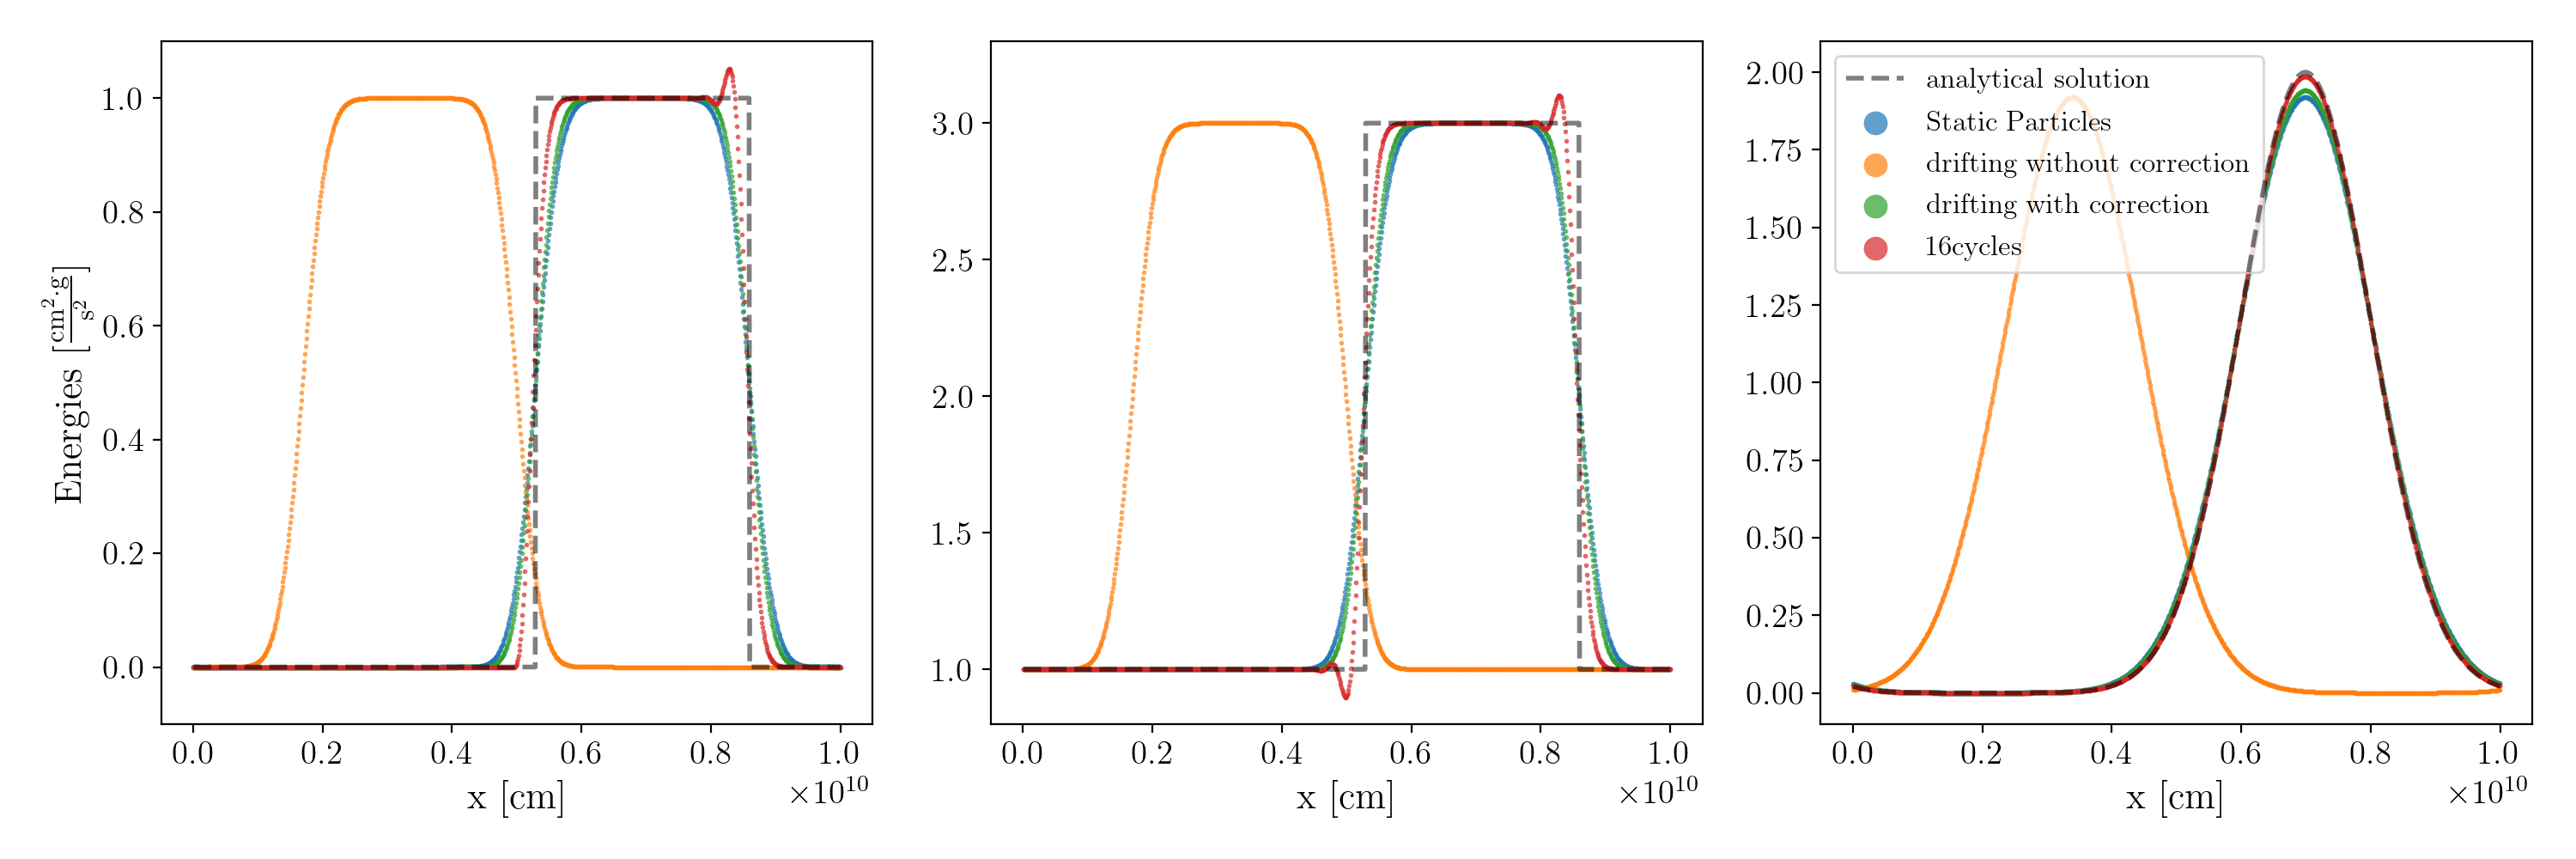
\includegraphics[width=\textwidth]{figures/RHD/drift/0.3c-16cycles.png}%
 \caption{
Results of the photon transport in a scenario where the fluid has a velocity of $-0.3c$ in
cases where particles are kept static (blue dots), when particles are drifted, but no drift
correction terms are applied (orange dots), when the drift correction terms are applied (green
dots), and when additionally 16 sub-cycles have been used (red dots).
 }
 \label{fig:drift-0.3c}
\end{figure}


\begin{figure}
 \centering
 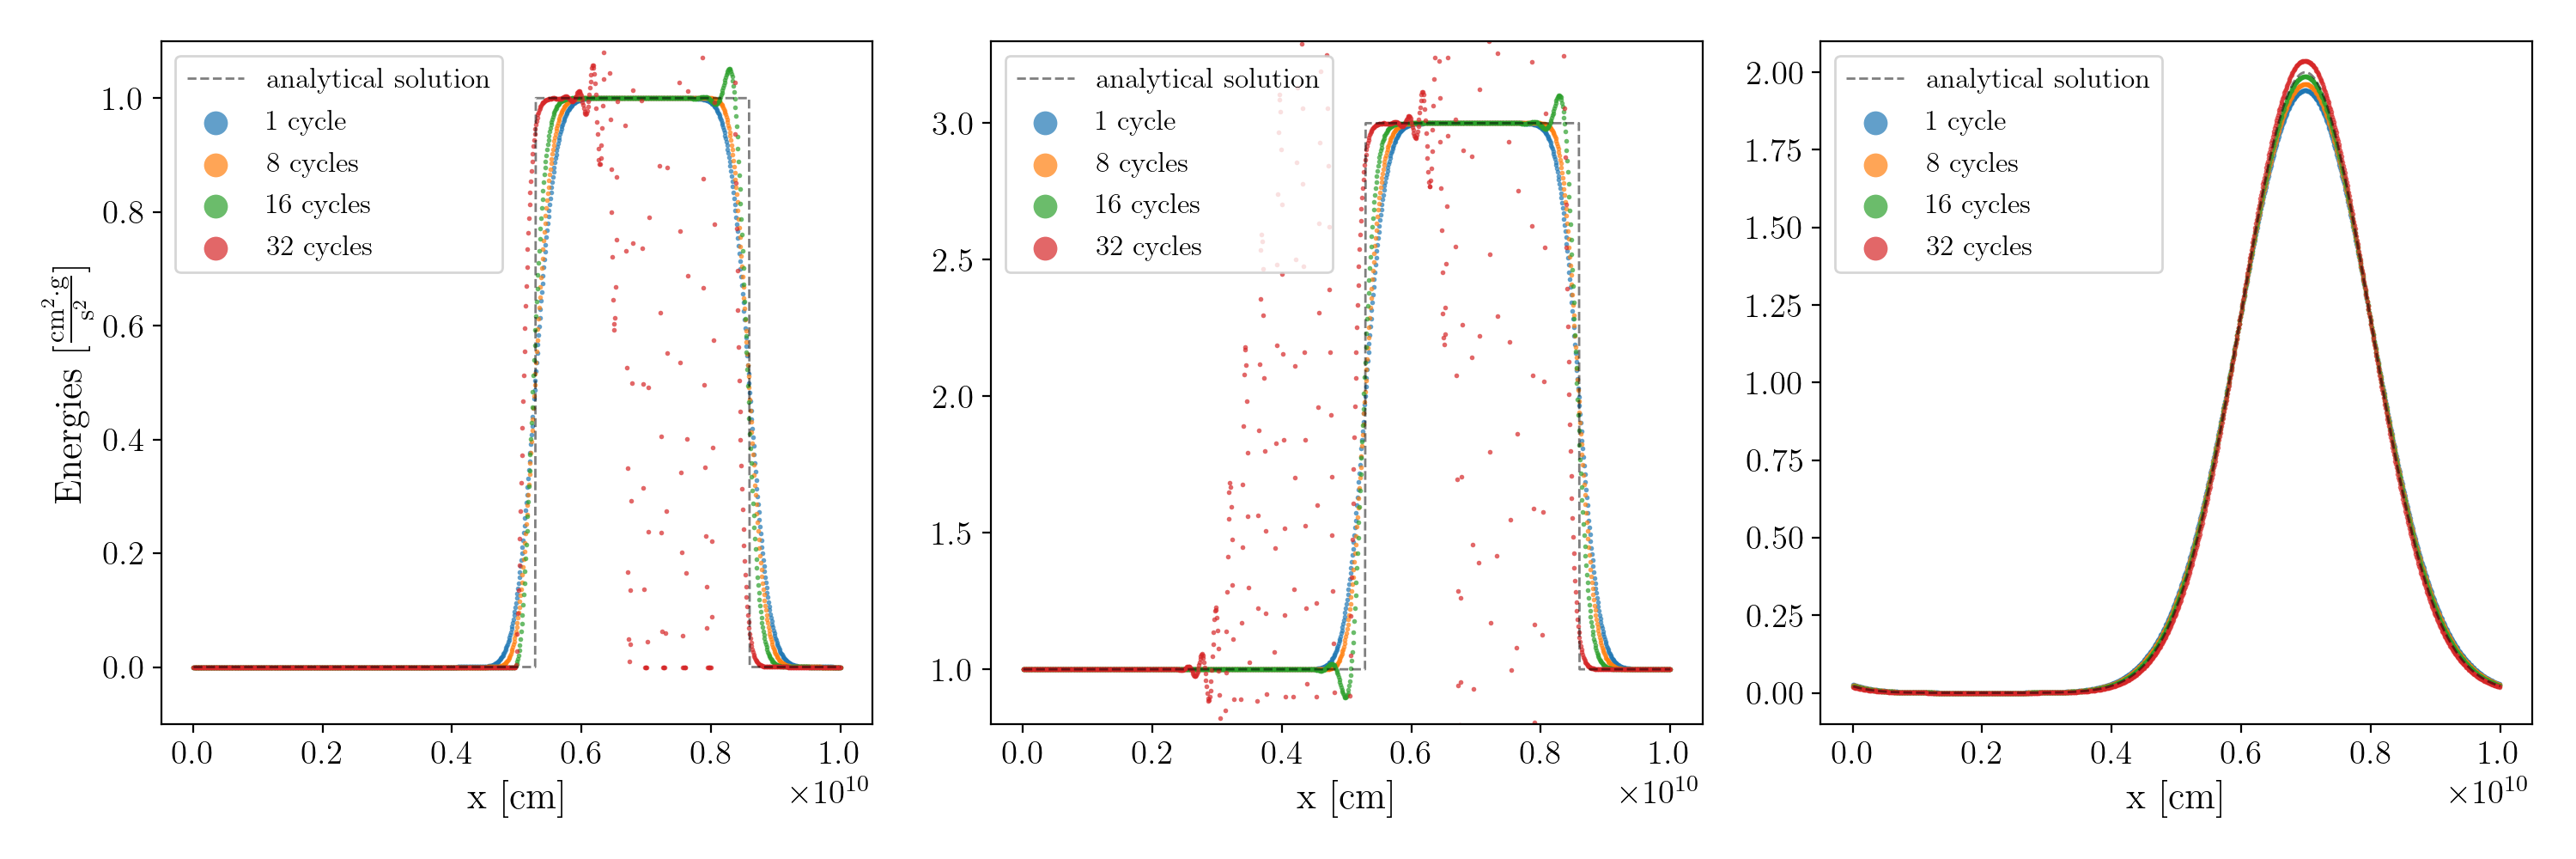
\includegraphics[width=\textwidth]{figures/RHD/drift/0.3c-subcycles.png}%
 \caption{
Same as Figure~\ref{fig:drift-0.3c}, but testing various numbers of sub-cycles along with the drift
correction. While higher sub-cycle numbers give catastrophic results, 8 sub-cycles still give
adequate results, even though they are above the realistic limit of 4 sub-cycles for a fluid
velocity of $-0.3c$.
 }
 \label{fig:drift-0.3c-subcycles}
\end{figure}




\begin{figure}
 \centering
 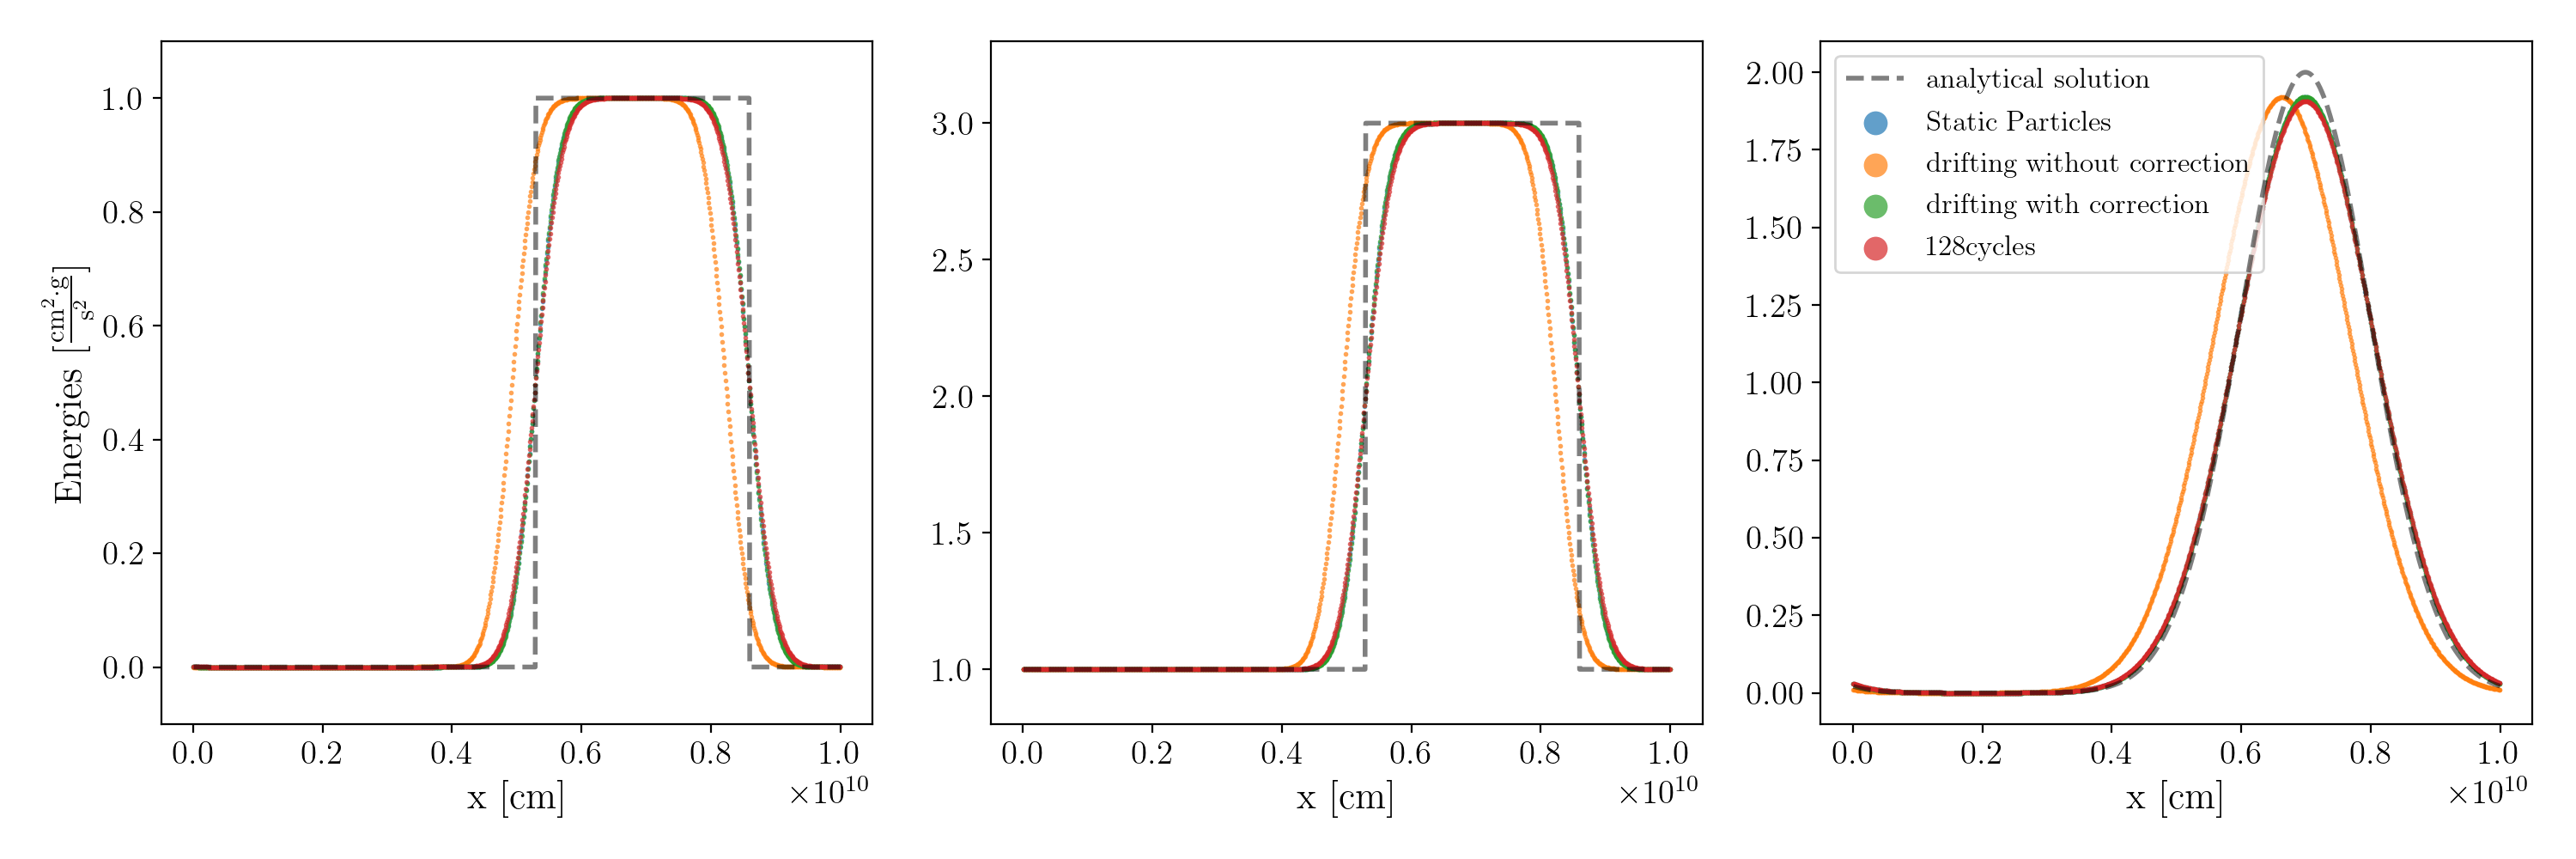
\includegraphics[width=\textwidth]{figures/RHD/drift/0.03c-128cycles.png}%
 \caption{
Same as Figure~\ref{fig:drift-0.3c}, but with a fluid velocity of $-0.03c$ instead of $-0.3c$. In
this case, even 128 sub-cycles don't develop instabilities.
 }
 \label{fig:drift-0.03c-subcycles}
\end{figure}



\begin{figure}
 \centering
 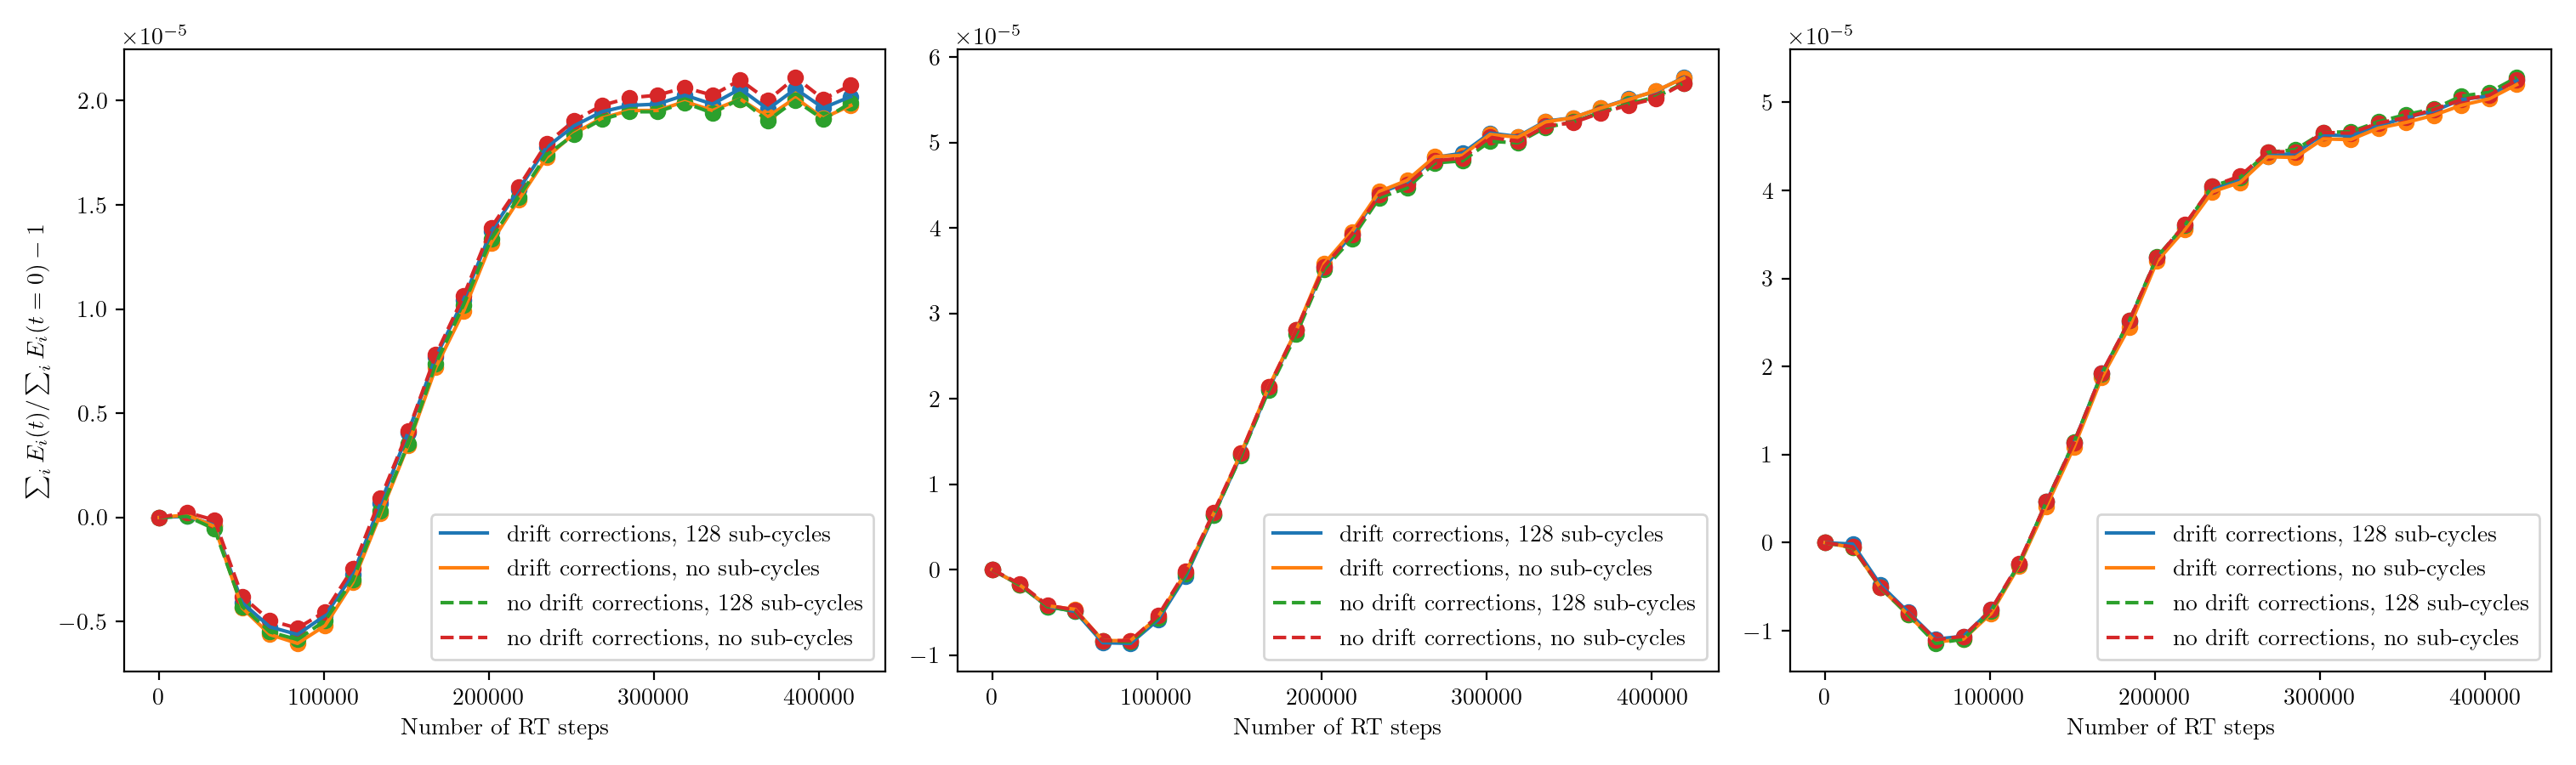
\includegraphics[width=\textwidth]{figures/RHD/drift/energy_comparison.png}%
 \caption{
The evolution of the total energy densities of slightly adapted initial conditions compared to
what is shown in Figure~\ref{fig:drift-0.3c}, as indicated in the main text, where the widths and
amplitudes of the initial functions have been tweaked in an attempt to introduce larger errors due
to the approximate drift correction scheme. The errors introduced by the approximate and not strictly conservative drift correction scheme remain within the order of the floating point precision, although they accumulate systematically over the course of hundreds of thousands of performed time steps, while remaining acceptably low.
 }
 \label{fig:drift-correction-conservation}
\end{figure}







As explained in Section~\ref{chap:rt-numerics-outline}, since the radiative transfer is solved as if
the particles were static interpolation points, but the particles are moved along with the fluid, a
correction term needs to be applied when particles are drifted. In this section, I test the validity
of that approach.

To this end, first an experiment in one dimension is set up as follows. As before, the photons
aren't allowed to interact with the gas, and are only transported. The initial conditions are (i) a
top hat function, (ii) a top hat function where the lower value is nonzero, and (iii) a smooth
Gaussian. The second top hat function with a nonzero lower value is used to test for cases where the
solution develops oscillations that would predict negative energy densities if the lower limit were
zero. In such cases \GEARRT would correct them, i.e. set the energy density to zero. By having a
nonzero lower value, these instabilities will show up.
The initial conditions are set up such that the radiation has fluxes of $\Fbf = c E$, i.e. the free
streaming limit, and the analytical solution is equal to a linear advection with constant
coefficients. The particles are given a velocity in negative $x$ direction, i.e. in the opposite
direction of the photon flux.

Figure~\ref{fig:drift-0.3c} shows the result for a particle velocity of $0.3c$. The following
results are shown:

\begin{itemize}
 \item The blue dots show the results when particles are kept static.
 \item The orange dots show the results when particles are drifted, but no correction terms are
applied. Clearly the radiation has been carried away by the particle drifts to the wrong position.
 \item The green dots show the results when particles are drifted along with the fluid, and the
correction terms discussed in Section~\ref{chap:rt-numerics-outline} are applied. The results agree
very well with the static particle case (blue dots).
 \item Finally, the red dots show the results for when the drift corrections are applied, and
additionally 16 RT sub-cycles have been used. The discontinuities develop an instability.
\end{itemize}

While the development of the instability with the sub-cycling may seem alarming at first, it is in
fact not a real problem. It develops because the sub-cycling allows for a larger hydrodynamics time
step, and hence a larger drifting distance. Because of the larger drift distance, the gradient
extrapolation then introduces new extrema which the limiters aren't able to keep in check any more.
However, 16 sub-cycles are not a realistic scenario, as the fixed number of 16 sub-cycles in
this case was enforced. In a real application, the number of sub-cycles would instead dynamically
adjust itself and be limited by the ratio of the speed of light to the particle velocity, in this
case 4. Indeed, Figure~\ref{fig:drift-0.3c-subcycles} compares the results for 1, 8, 16, and 32
sub-cycles, and the results for up to 8 sub-cycles are perfectly adequate.
Figure~\ref{fig:drift-0.03c-subcycles} shows the results with a ten times lower fluid velocity of
$-0.03c$, where even 128 sub-cycles show no trace of an instability developing. Tests with similar
setups in 2D confirm these findings, and I conclude that using gradients of the radiation quantities
to extrapolate their values in order to deal with particle drifts is an adequate approach.



A caveat of the correction scheme for particle drifts is that the method to solve radiation
transport is no longer strictly conservative. However, testing the radiation energy density
conservation explicitly by comparing the current total energy densities with the initial ones shows
that the introduced errors are negligibly small and within the precision limits of the single
precision floating point variables used to carry the radiation fields.
Figure~\ref{fig:drift-correction-conservation} shows the results of such a comparison for a test
similar to the experiment setup previously described in this section: We transport two top hat
functions, one of which has a nonzero lower value, and a smooth Gaussian function. The amplitude of
the Gaussian and the upper value of the top hat function have been increased by a factor of 5,
while
their width has been reduced to take one fifth of the box size in an attempt to produce sharper
discontinuities which will require more time for the diffusivity of the method to smooths them out
significantly, therefore keeping steeper gradients for longer. Additionally, in an attempt to
increase the distances of each drift, the ratio of the speed of light to the gas (drift) velocity
was set to -40. Varying these parameters (amplitudes and widths of initial conditions,
ratio of speed of light to drift velocity), as well as the number of particles used all had
negligible effect on the outcome with regards to total energy conservation: The errors remain
within the precision limits of the floating point numbers (although they accumulate systematically
over the course of hundreds of thousands of performed time steps, while remaining acceptably low).
As such, I deem the drift correction scheme as appropriate for use without any further corrections
or adaptations.







%===============================================================================================
\section{Testing Injection Models From Radiation Sources}
%===============================================================================================


%-----------------------------------------------------------------------------------------------
\subsection{Testing Flux Injection Models From Radiation Sources}\label{chap:results-injection}
%-----------------------------------------------------------------------------------------------

\begin{figure}
 \centering

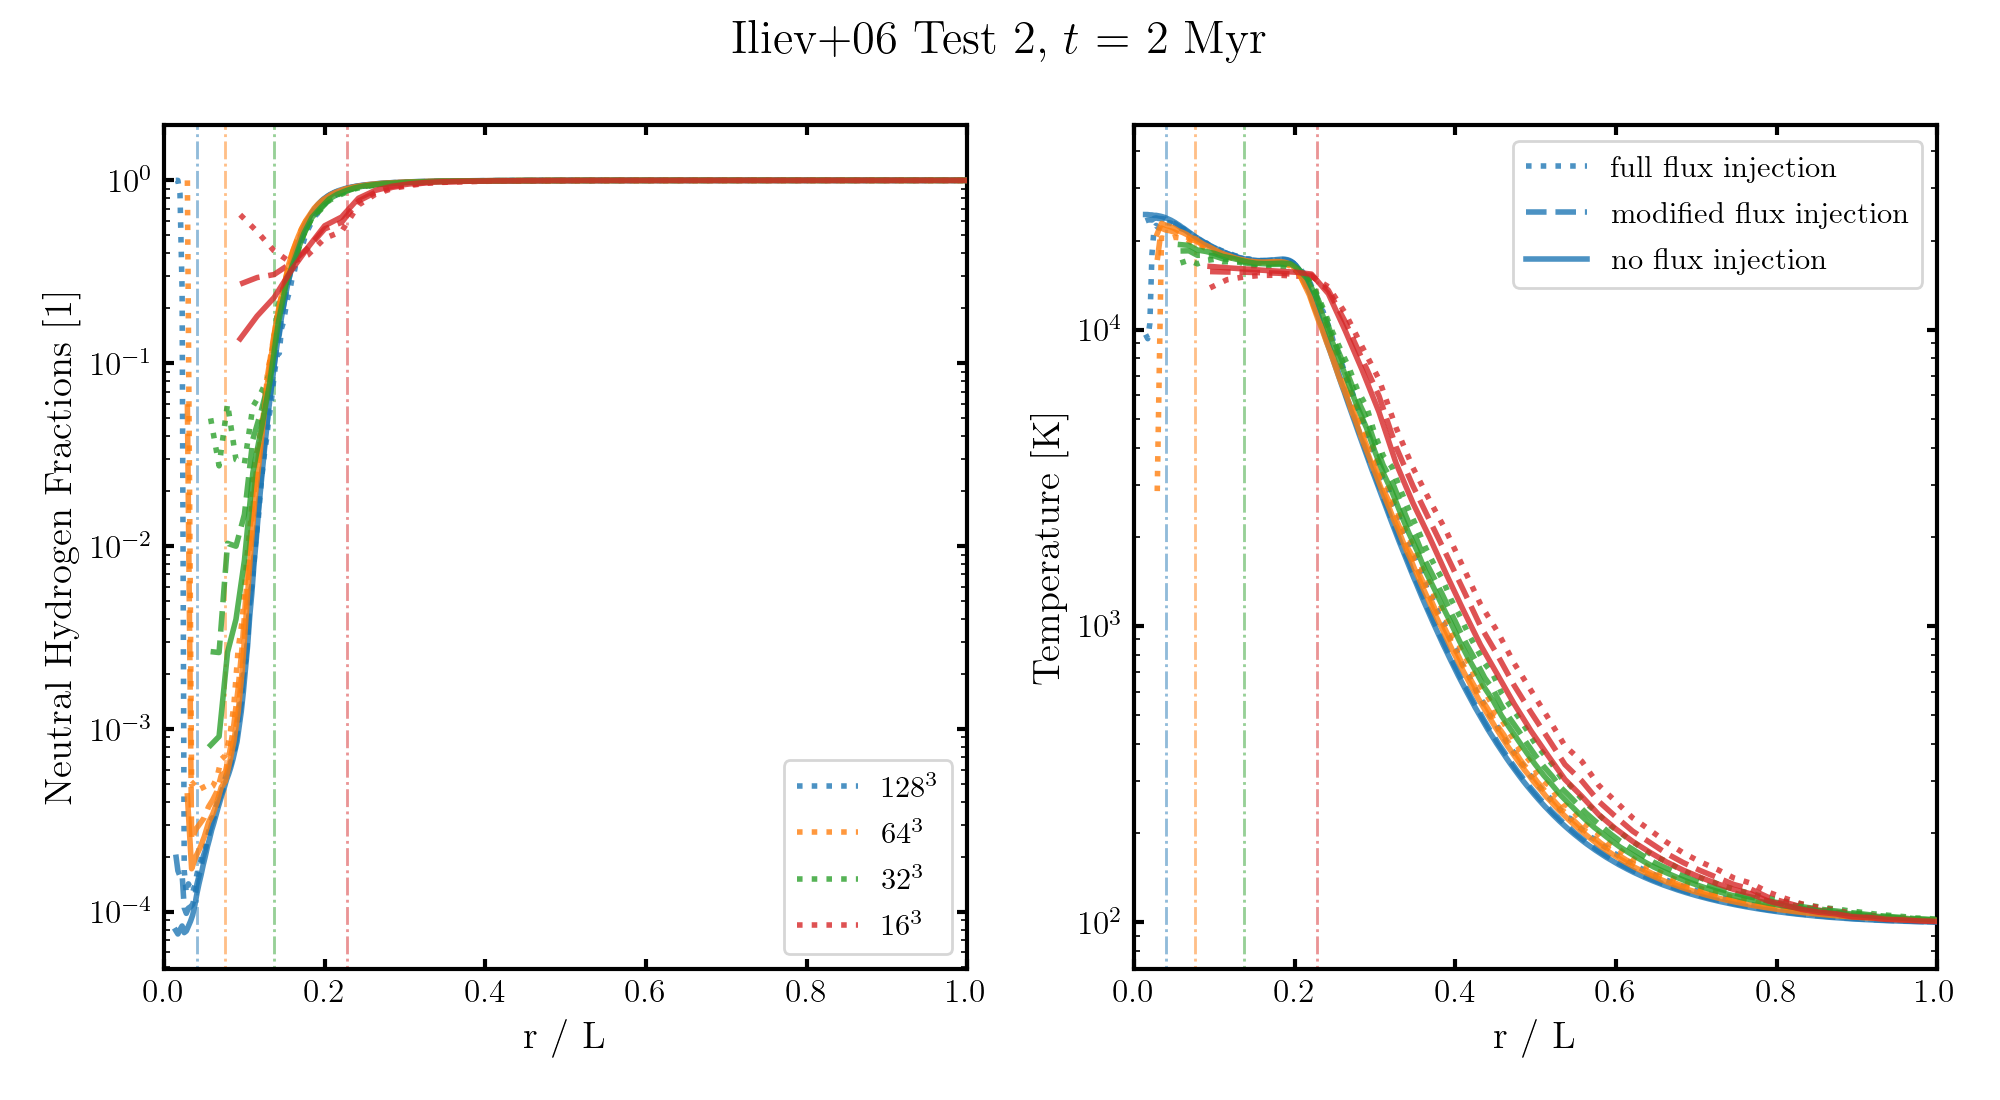
\includegraphics[width=\textwidth]
{figures/RHD/injection_models/injection_convergence_test_2Myr.png}
\\
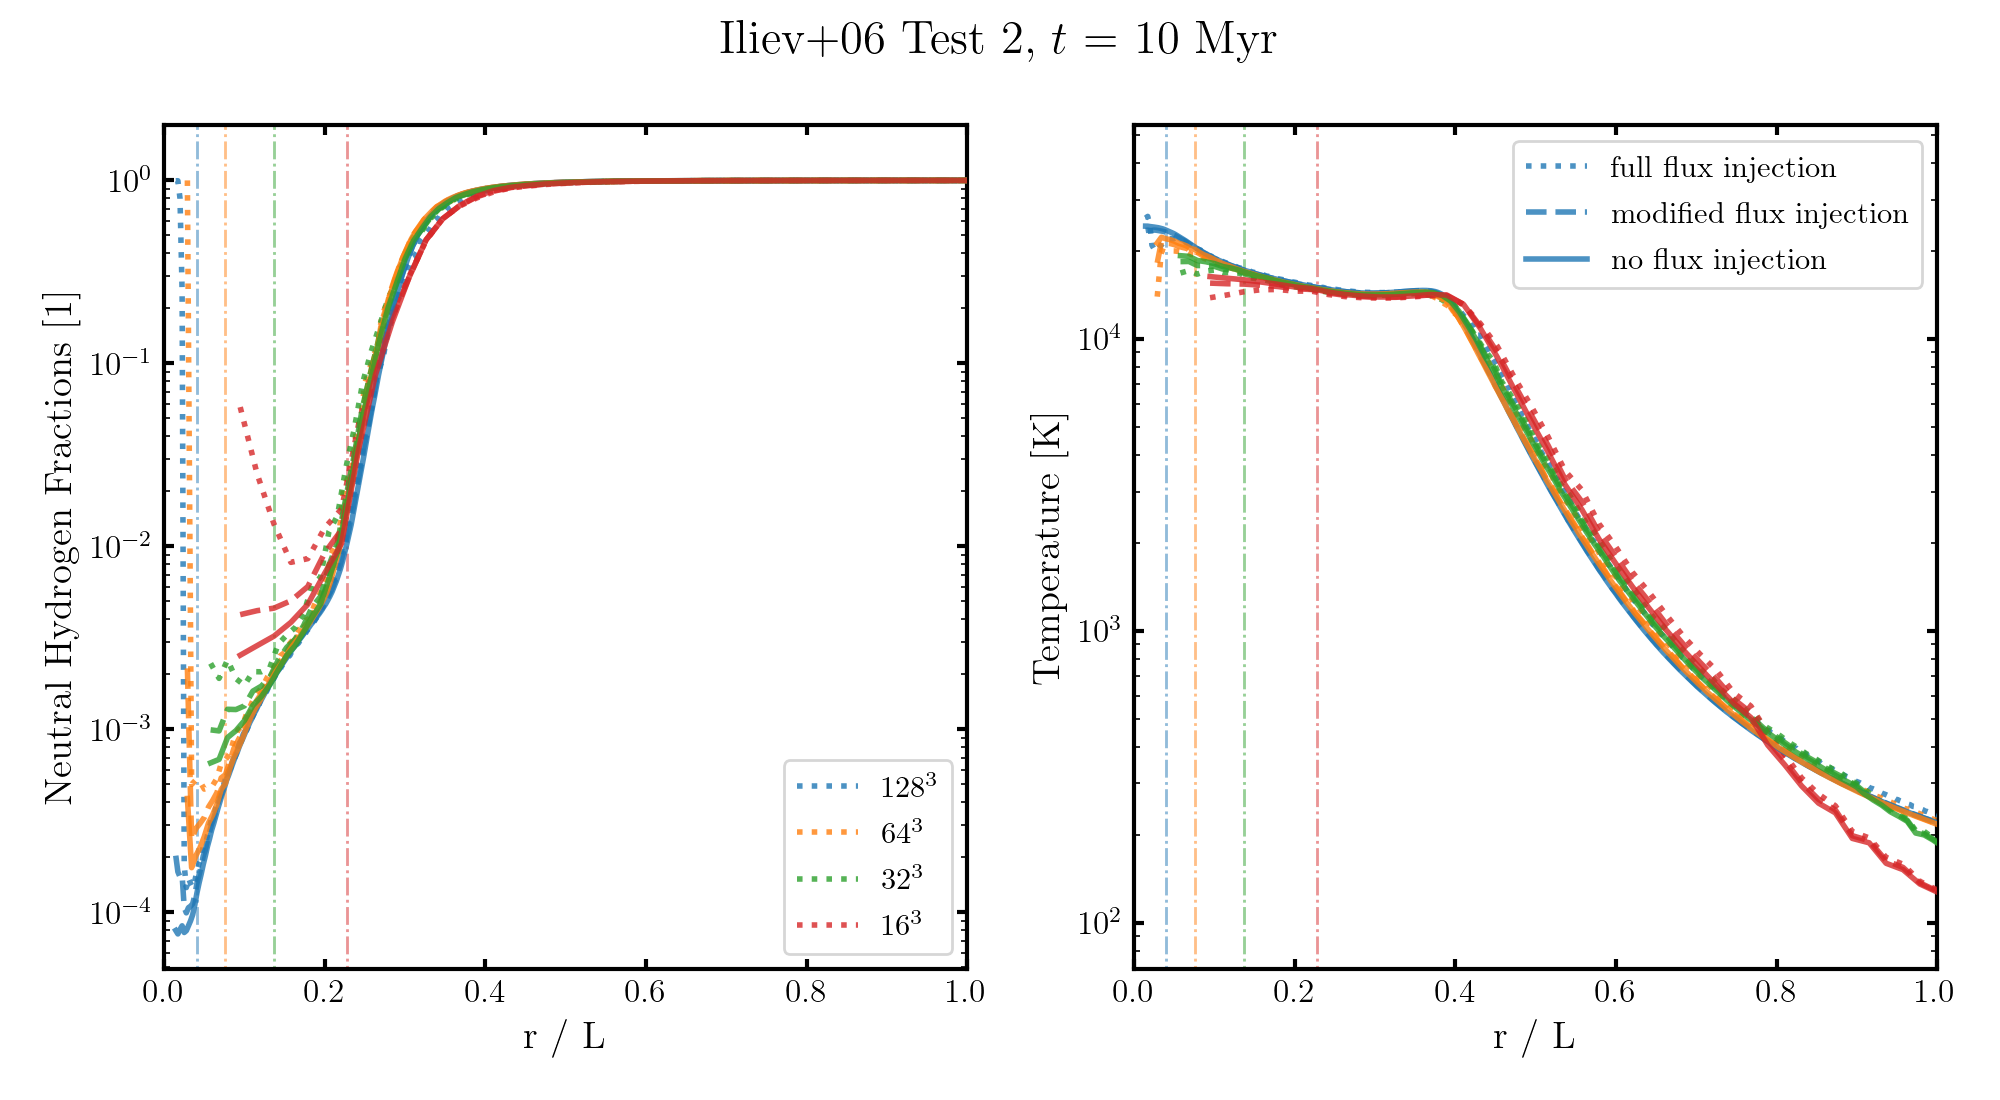
\includegraphics[width=\textwidth]
{figures/RHD/injection_models/injection_convergence_test_10Myr.png}
\caption{
Radial profiles of the results of the Iliev 2 test (see Section~\ref{chap:Iliev2} for details) for
varying flux injection methods and resolutions, as indicated in the legends, at $t = 2$Myr (top)
and $t = 10$Myr (bottom). The vertical dash-dotted lines show the maximal radius at which energy
and fluxes are injected from a source, which is located at $r = 0$, for the various resolutions.
 }
 \label{fig:injection_convergence}
\end{figure}


\begin{figure}
\centering
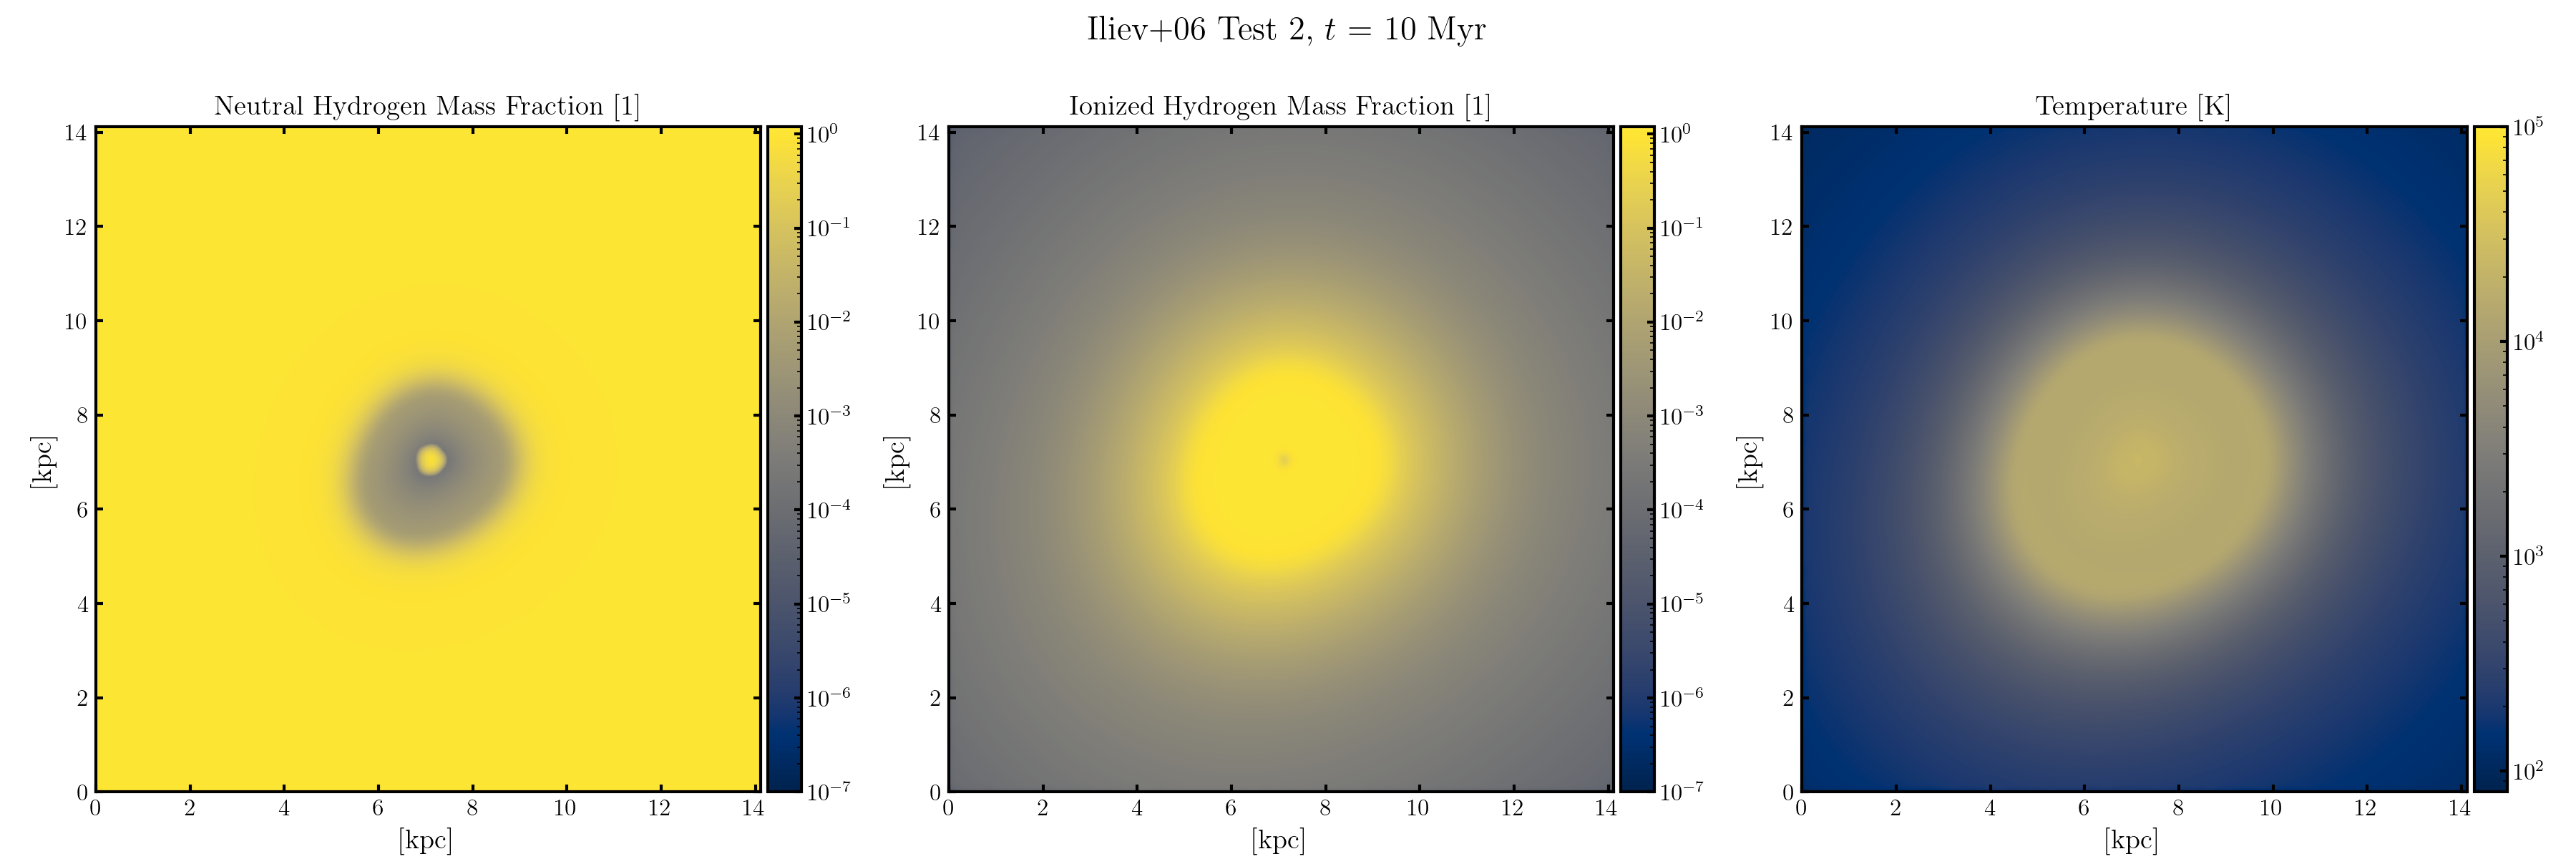
\includegraphics[width=\textwidth]
{figures/RHD/injection_models/injection_convergence_test_FullFlux128.png}\\
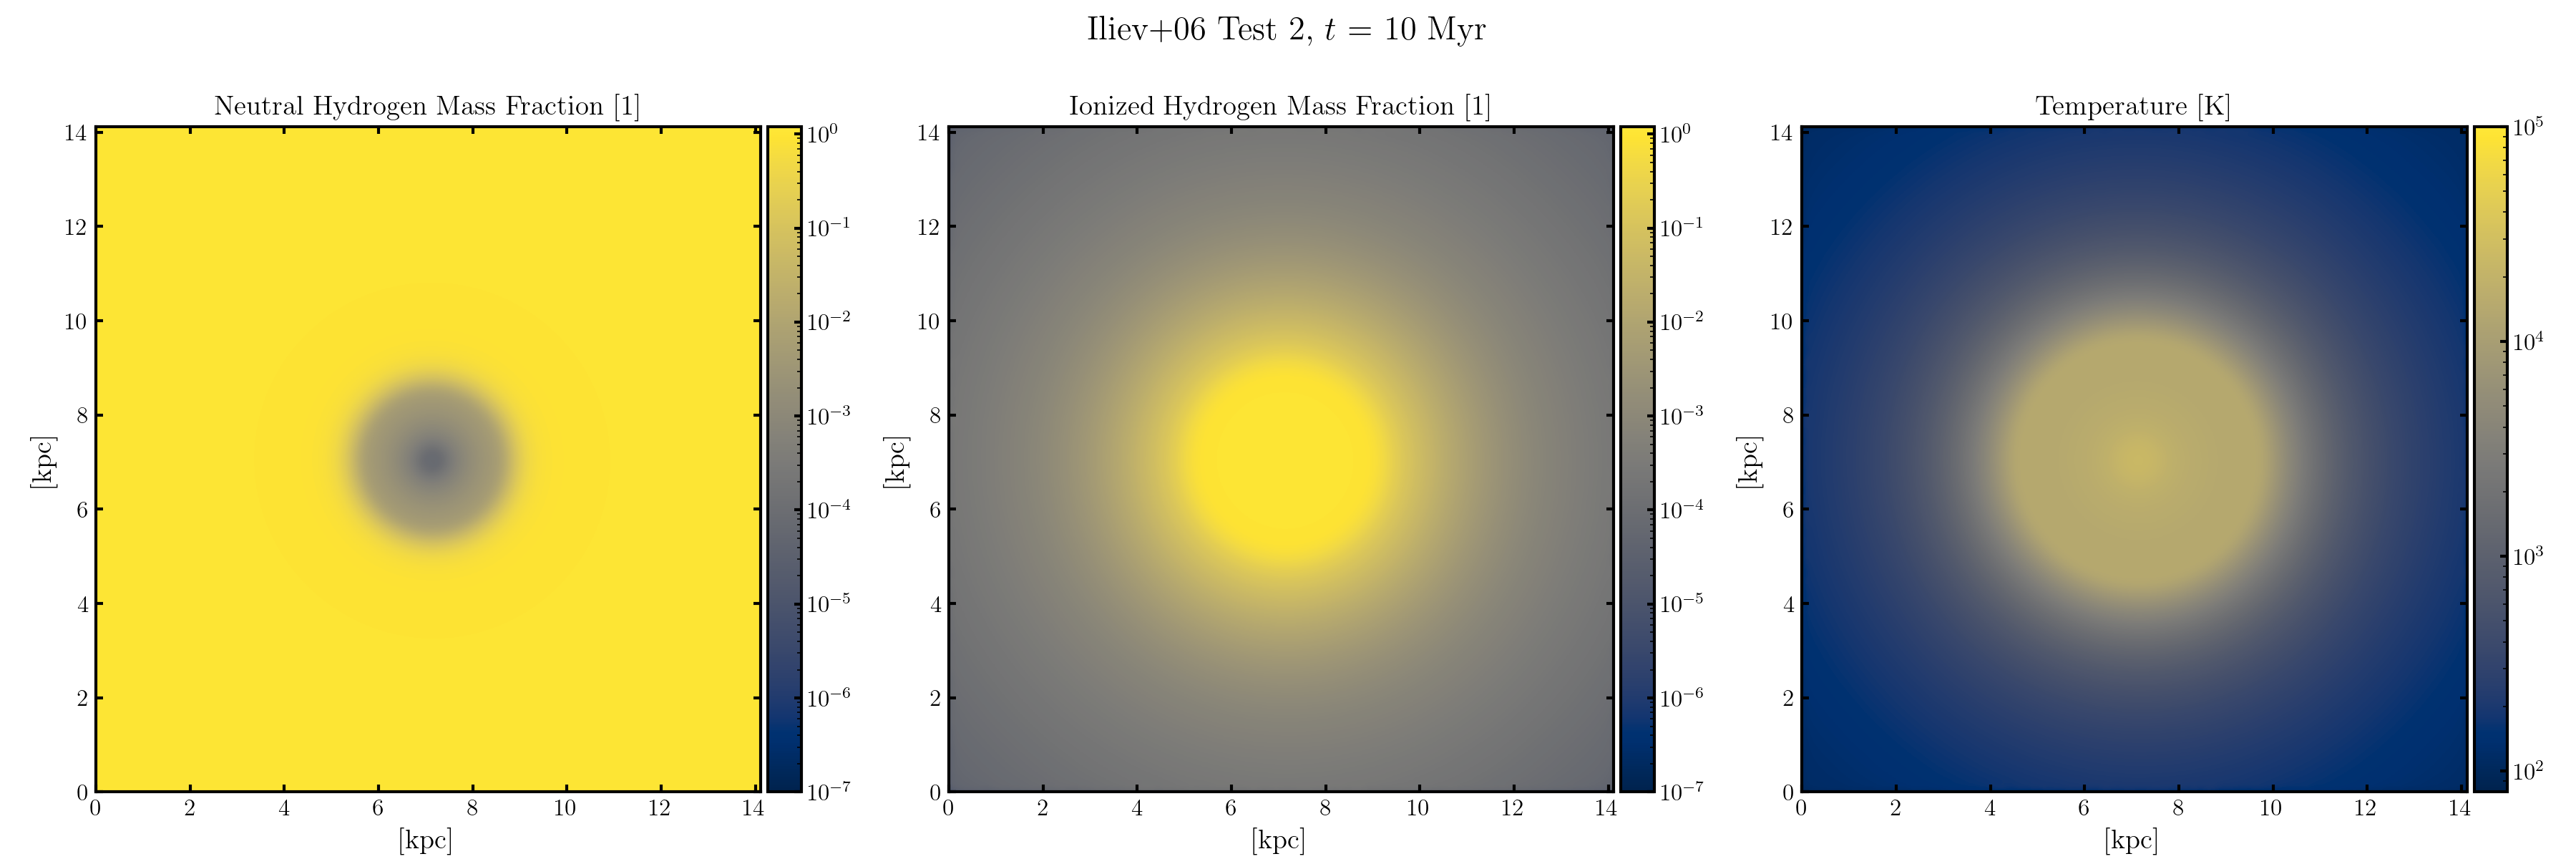
\includegraphics[width=\textwidth]
{figures/RHD/injection_models/injection_convergence_test_NoFlux128.png}
\caption{
Slice along the mid-plane of the results of the Iliev 2 test (see Section~\ref{chap:Iliev2} for
details) for the ``full flux injection'' model (top) and the ``no flux injection'' model (bottom)
in the $128^3$ particle simulation at $t = 10$Myr. The ``full flux injection'' model transports
too much radiation energy density away from the innermost regions of the box, leaving the immediate
vicinity of the radiation source under-ionized.
 }
 \label{fig:flux-injection-slices}
\end{figure}




In this section, three different ways of injecting radiation \emph{flux} are tested, as mentioned in
Section~\ref{chap:injection-step}. Contrary to mesh based codes, where the net injected flux from a
point source radiating isotropically inside a single cell always neatly sums up to zero, \GEARRT is
a particle based code, and radiation is injected into a group of particles. This leaves us with
some freedom to choose how exactly to inject the photon fluxes onto the particles, while still
maintaining that the vector sum of the injected fluxes should remain zero to preserve isotropy.
Three flux injection models are tested:

\begin{itemize}
 \item The ``no flux injection'' model injects no radiation flux $\Fbf$, i.e. only energy density
is injected onto particles.
 \item The ``full flux injection'' model injects flux assuming an optically thin limit, i.e. $\Fbf
= c E$
 \item The ``modified flux injection'' model injects a linearly increasing amount of flux
with increasing distance starting with no flux and ending in the optically thin limit $\Fbf = c E$
at the distance $0.5H$, where $H$ is the maximal distance at which energy and flux is injected. For
distances above $0.5H$, again the value of the optically thin limit is taken.
\end{itemize}

Note that the anisotropy correction terms for the injection of energy density described in
Section~\ref{chap:injection-weights} are also applied here for all flux injection models.

The test setup is identical to the Iliev 2 test, which is described in detail in
Section~\ref{chap:Iliev2}. For the scope of this section however, it suffices to note that the test
consists of a single ionizing source injecting photons into its uniform surroundings. The
temperature and ionization state of the gas is only modified through the influence of the radiation,
actual hydrodynamics are turned off.


Figure~\ref{fig:injection_convergence} shows the results at 2 Myr and at 10 Myr using various
resolutions, ranging from $16^3$ to $128^3$ particles. The strongest deviations are within the
region where energy density is injected, i.e. within the compact support radius $H$ of the source,
beyond which the solutions for all resolutions and flux injection methods converge quickly.

The ``full flux injection'' model and the ``modified flux injection'' model are somewhat
problematic, as they leave a peak in neutral hydrogen fraction and a dip in temperature very close
to the source (which is located at $r = 0$), whereas the solution is expected to be monotonously
increasing in the neutral hydrogen fraction and decreasing in the temperature, respectively.
Essentially the immediate vicinity around the source remains under-heated and under-ionized. The
reason for this phenomenon lies in the order of operators used in the operator splitting scheme to
solve the equations of radiative transfer: The photon transport is done before the thermochemistry.
With a flux corresponding to the free streaming limit, too much energy is being transported away
before it can heat and ionize the gas sufficiently in the thermochemistry step. This is supported by
the fact that the ``no flux'' model indeed delivers the best results. The lack of ionization and
heating in around the source can be seen very clearly in Figure~\ref{fig:flux-injection-slices},
where the a slice through the mid-plane of the box is shown for the solution of the ``full flux'' and
the ``no flux'' models. Additionally, Figure~\ref{fig:flux-injection-slices} shows that the ``full
flux'' model exacerbated anisotropies in the ionized region, adding a further reason to prefer to
avoid it.

With an increasing amount of flux injected into the gas, the gas heats up a little more at large
distances. The difference is negligible though, and decreases with increasing resolution. As such,
it is safe to conclude that the amount of flux injected from a single source is not really relevant
for regions far from the source. Indeed, even when injecting only energy density and no flux at all
particles ``develop'' a flux in the subsequent time step (see
Appendix~\ref{app:zero-flux-nonzero-energy}). Given how injecting zero flux leads to best results
close to the source, and to negligible differences far from the source, I recommend that model to
be used.\footnote{
In fact, the flux injection method is not left to users as a free parameter for \GEARRT, but the
``no flux'' model is used as the default and only choice.
}








%-----------------------------------------------------------------------------------------------
\subsection{Testing Different Time Step Sizes for Injection and Radiation Transport}
\label{chap:results-star-timesteps}
%-----------------------------------------------------------------------------------------------



\begin{figure}
\centering
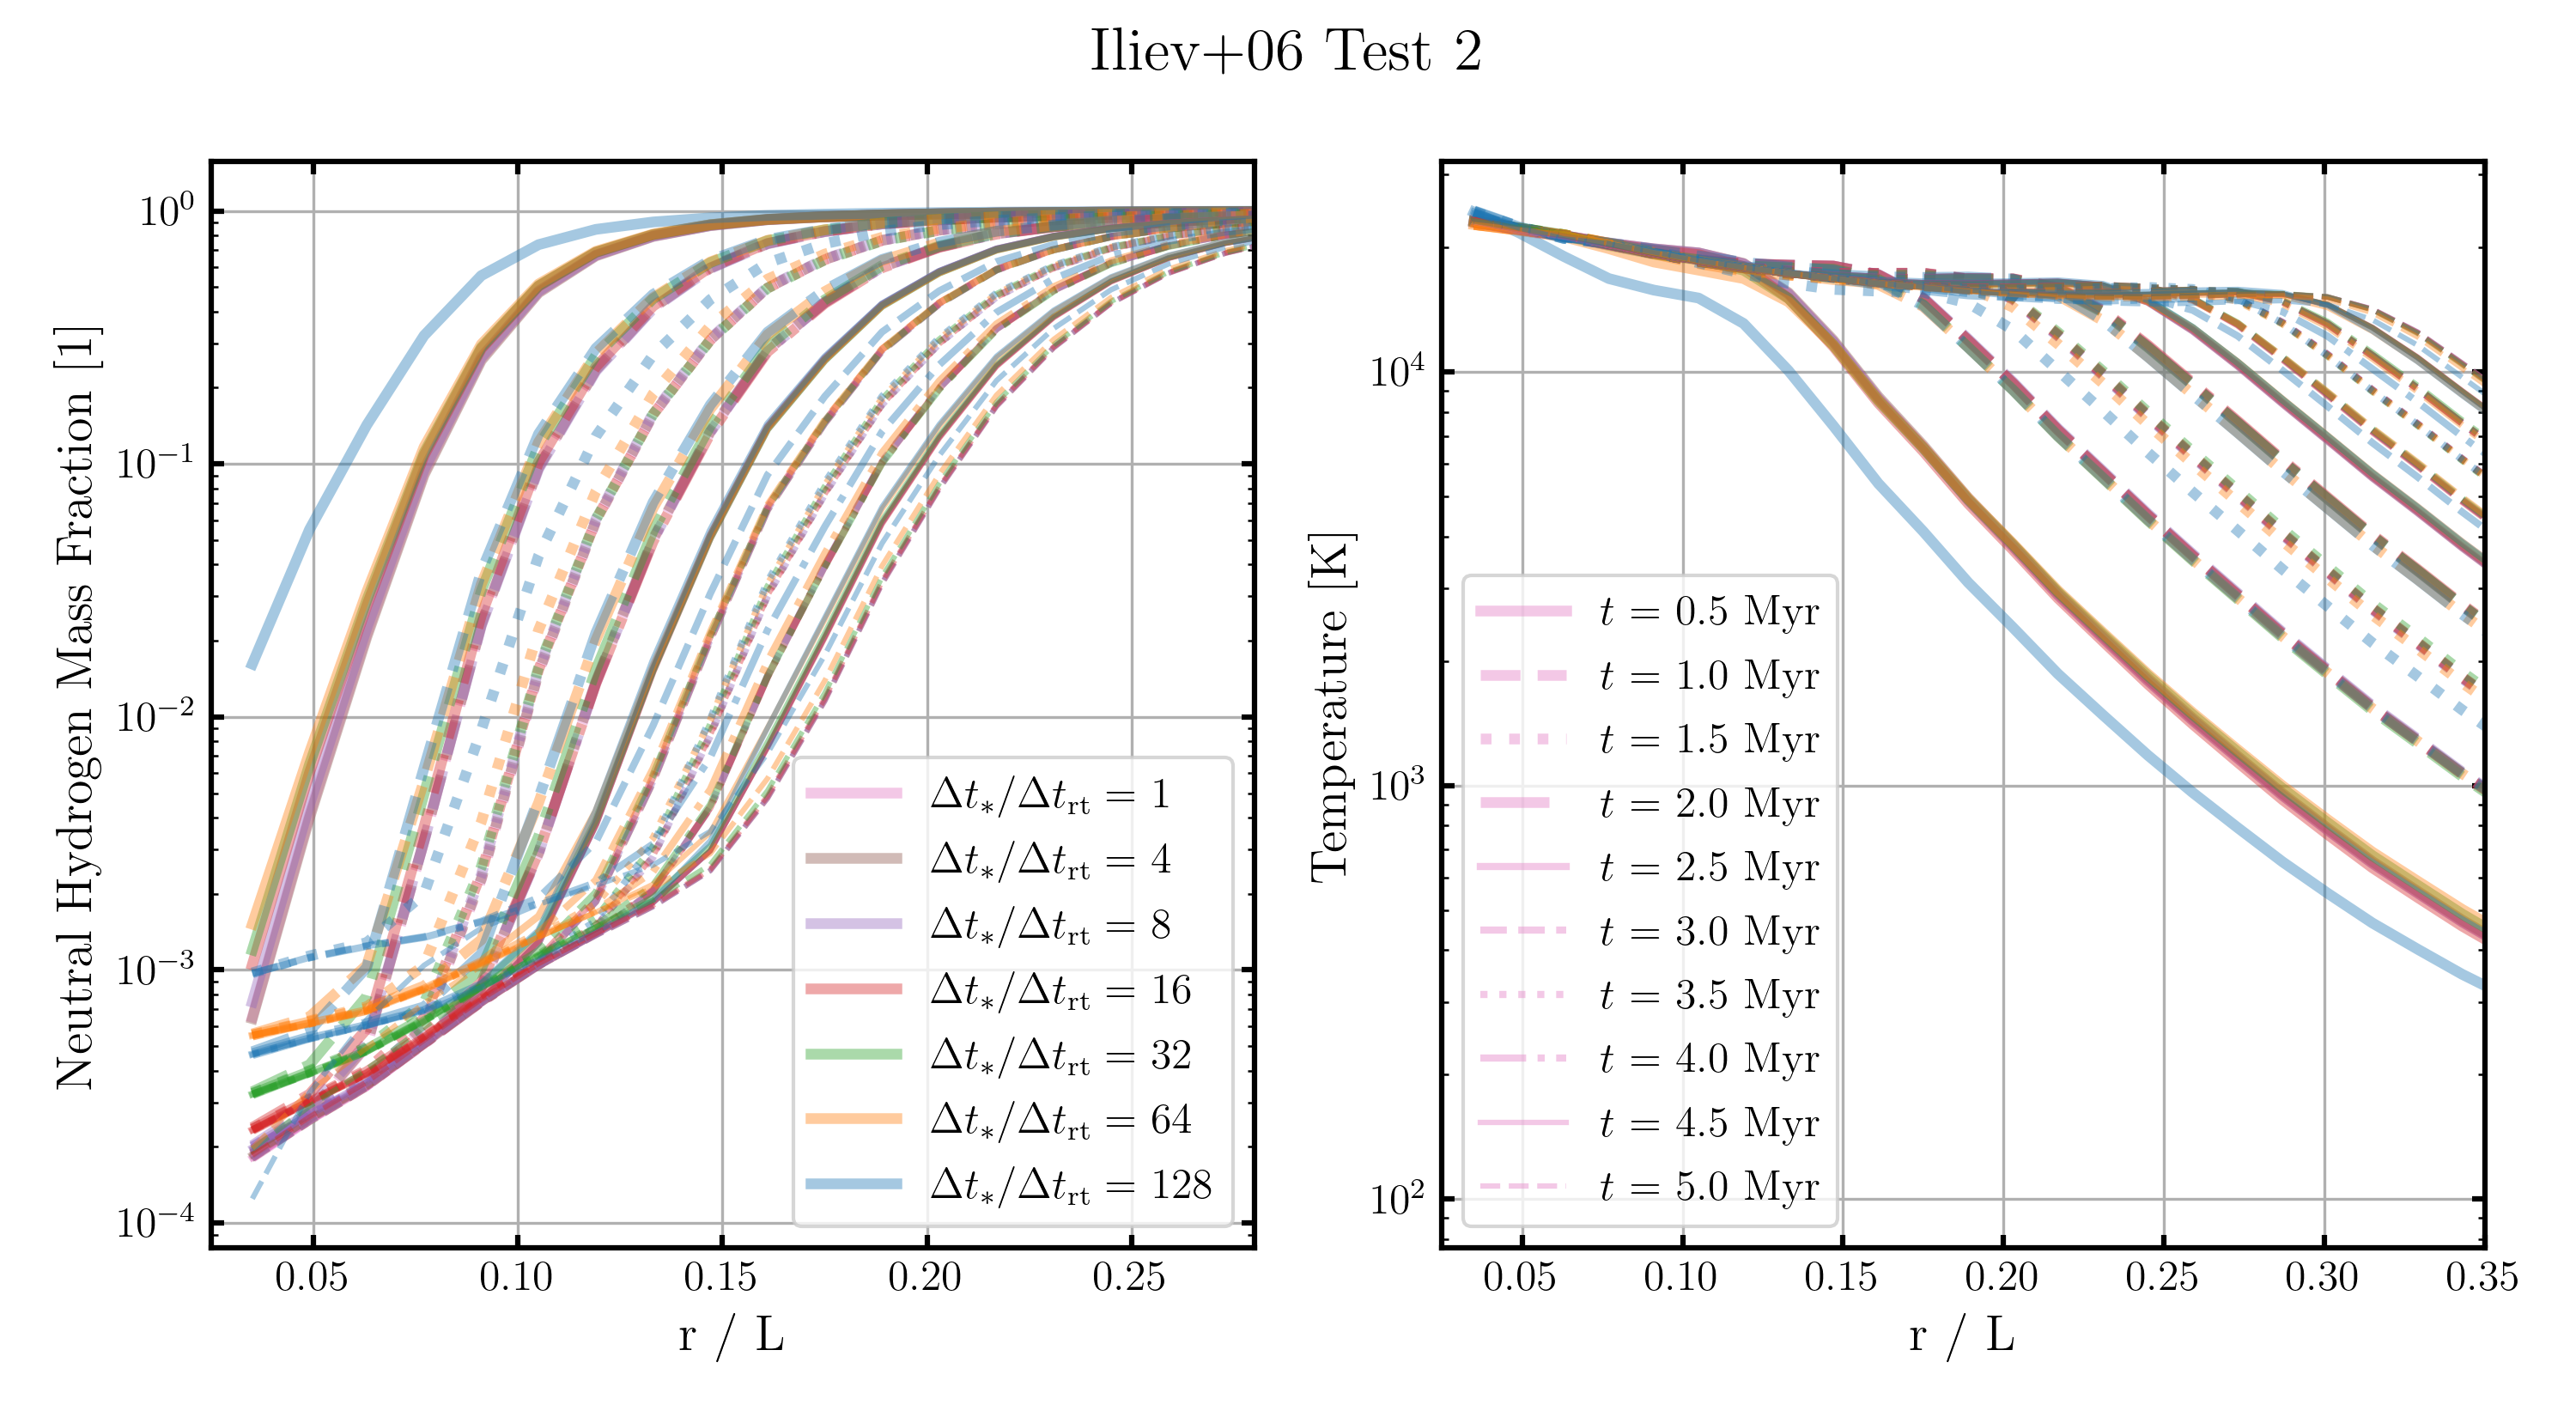
\includegraphics[width=\textwidth]{figures/RHD/injection_timesteps/compareProfiles.png}%
\caption{
Profiles of the neutral hydrogen mass fractions and the gas temperature over time for increasing
power-of-two multiples of star time step sizes $\Delta t_*$ compared to the radiative transfer time
step size $\Delta t_{\mathrm{rt}}$ for initial conditions identical to the Iliev Test 2 (see
Section~\ref{chap:Iliev2} for details). The colors of the lines represent a specific ratio $\Delta
t_* / \Delta t_{\mathrm{rt}}$, while the line widths and styles depict the results at different
times, as indicated in the legends.
}
\label{fig:injection-timesteps-profiles}
\end{figure}


\begin{figure}
\centering
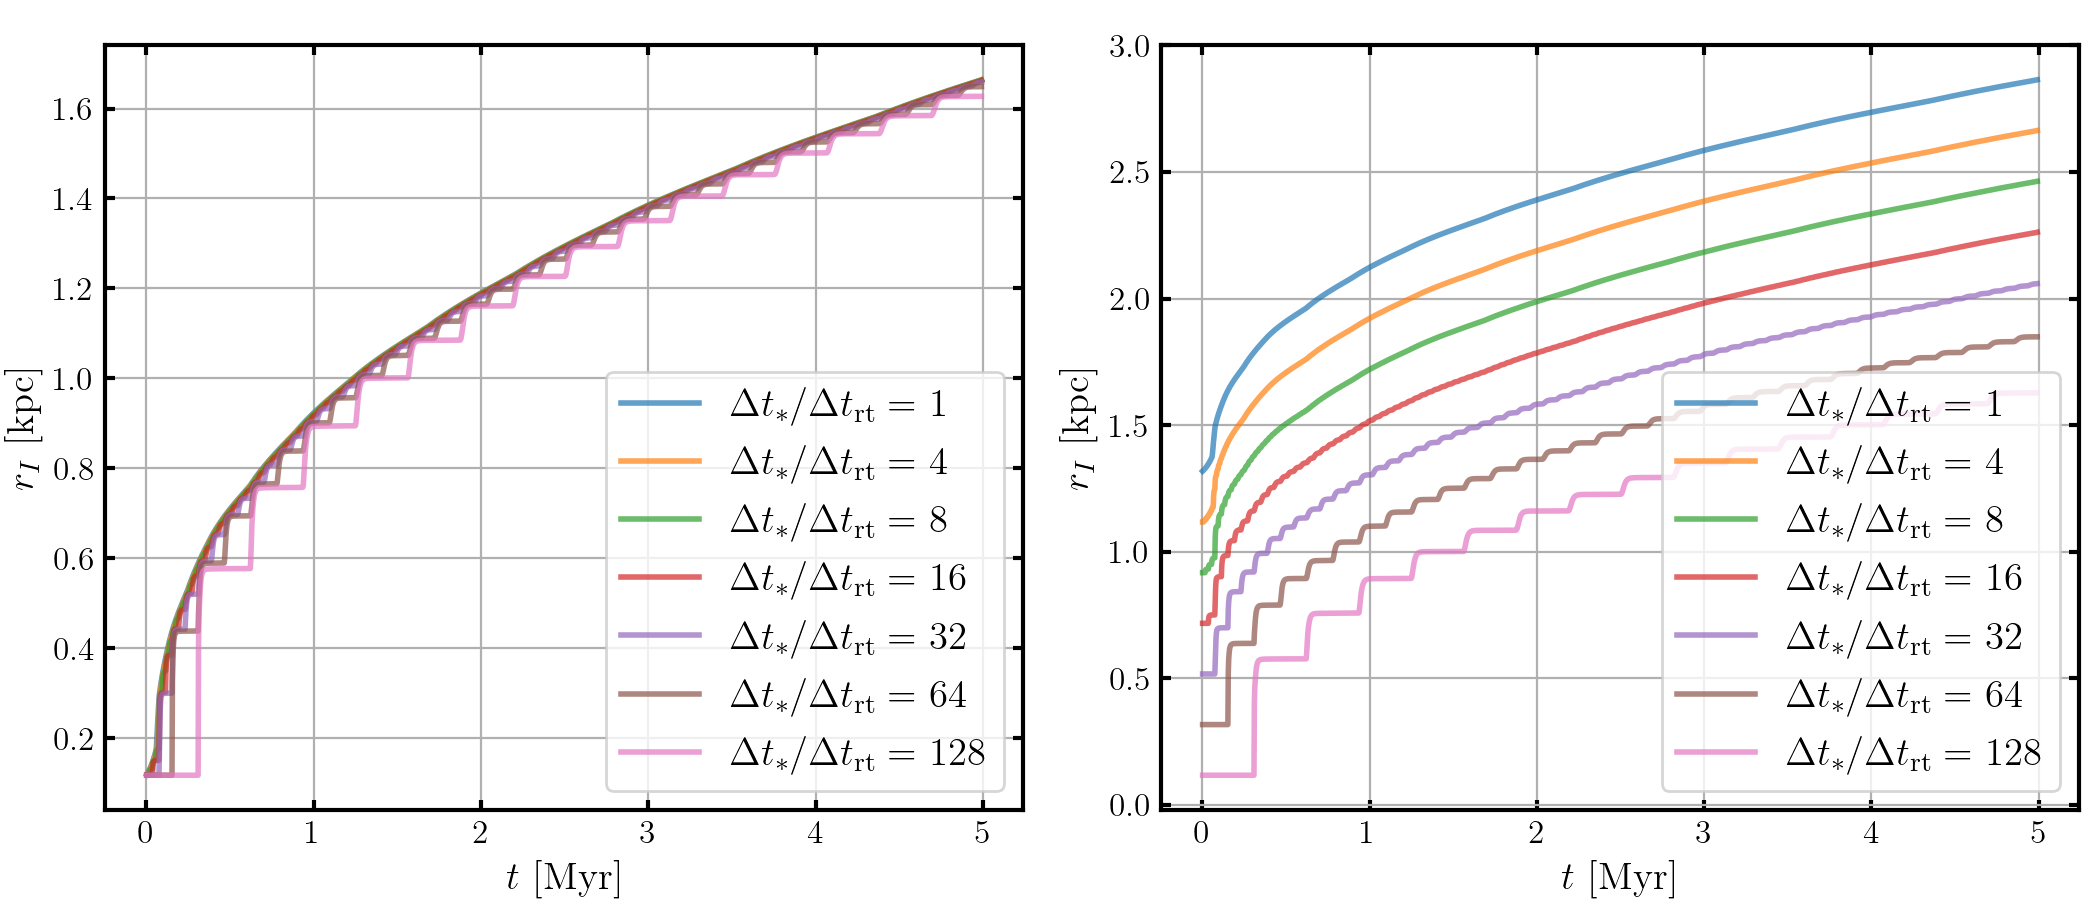
\includegraphics[width=\textwidth]{figures/RHD/injection_timesteps/ionization_fronts.png}%
\caption{
Position of the radius of the ionization front, defined as the point where the ionized hydrogen mass
fraction is one half, over time for increasing power-of-two multiples of star time step sizes
$\Delta t_*$ compared to the radiative transfer time step size $\Delta t_{\mathrm{rt}}$ for initial
conditions identical to the Iliev Test 2 (see Section~\ref{chap:Iliev2} for details). The right
plot is the same as the left plot, but with a displacement of $0.2$kpc added between each ratio
$\Delta t_* / \Delta t_{\mathrm{rt}}$ so each individual line can be seen clearly.
}
\label{fig:injection-timesteps-ionization-front-radius}
\end{figure}



As mentioned before, particles are permitted to have individual time step sizes (which must be
multiples-of-two of some global minimal time step size). While this is true for gas particles
compared to each other, it is also true between star particles and gas particles. This means that
the photon injection step, which is determined by the star particles' time step sizes, can and will
be performed less frequently\footnote{In principle, the injection step can also occur \emph{more}
frequently than the transport step, but this is not a situation we'd need to be concerned about at
all. Star particles having time step sizes smaller than radiative transfer time step sizes
is not really a realistic scenario, and as such is not expected to occur at all. If it does occur
at any point, the injected energy density will just be added to the neighboring gas particles
several times instead of only once, where the total sum of the injected energy density remains
identical. So the injection of radiation energy density in the situation where a star particle has
a smaller time step size than its neighboring gas particles results in the identical outcome as if
it had the same time step size as the gas particles.}
than the photon transport steps, who in turn are determined by the gas particles' RT time step sizes
(see Section~\ref{chap:injection-step}).


To test the influence of increasing time step sizes of star particles, I use the same setup as in
the previous section, which is also identical to the Iliev 2 test, described in detail in
Section~\ref{chap:Iliev2}. For the scope of this section however, it suffices to note that the test
consists of a single ionizing source injecting photons into its uniform surroundings. The
temperature and ionization state of the gas is only modified through the influence of the radiation,
actual hydrodynamics are turned off.

Figure~\ref{fig:injection-timesteps-profiles} shows the resulting profiles of the neutral hydrogen
mass fractions and the gas temperature over time for increasing powers-of-two of star time step
sizes compared to the radiative transfer time step size. The profiles with time step ratios $\Delta
t_* / \Delta t_{\mathrm{rt}} \leq 32$ agree quite well with each other save for the innermost
region $r / L \lesssim 0.075$, where smaller ratios find an increasingly lower neutral hydrogen
mass fraction. This is also the region closest to the radiation source, and it is to be expected
that it would react the most sensitively to a change in the frequency of energy density injection.
The differences in the neutral hydrogen mass fraction for the ratios $\Delta t_* / \Delta
t_{\mathrm{rt}} \leq 32$ are rather small, with a maximum of a factor of $\sim 2$ closest to the
source for $\Delta t_* / \Delta t_{\mathrm{rt}} = 32$, and the profiles become virtually identical
at $r / L \gtrsim 0.075$. This distance is also roughly the compact support radius of the star
particle, within which particles are injected with radiation energy density, and in the context of
radial profiles a rather poorly resolved region. As such, these differences are deemed
unproblematic.

The situation is different for higher ratios $\Delta t_* / \Delta t_{\mathrm{rt}} = 64$ and $128$.
They show clear differences to other profiles. In particular the ratio 128: At 0.5 Myr, it lags
behind other profiles. At 1 Myr, it has caught up with them again, only to lag behind again at 1.5
Myr. This cycle repeats for later times as well. The situation becomes more clear when we look at
the evolution of the ionization front radius over this time span. The ionization front radius is
defined as the radius at which the ionized hydrogen mass fraction is exactly half. It's evolution
through time is shown in Figure~\ref{fig:injection-timesteps-ionization-front-radius} for the same
ratios $\Delta t_* / \Delta t_{\mathrm{rt}}$ as shown before. Here, the influence of the increasing
time intervals between two energy density injections is obvious. For larger time step size ratios,
the ionization front radius expands almost instantaneously after each injection, and then remains
static until the next injection occurs, leading to the step-like curves that can be seen in
Figure~\ref{fig:injection-timesteps-ionization-front-radius}. The step sizes decrease proportionally
to the decreasing time step size ratios, and also decrease with the distance of the ionization
front radius from the source. For  $\Delta t_* / \Delta t_{\mathrm{rt}} = 8$, the steps are only
detectable at early times $t < 0.5$ Myr, while for  $\Delta t_* / \Delta t_{\mathrm{rt}} = 16$,
they are visible until $t \sim 2$ Myr.

The step-wise ionization for higher time step size ratios (save for perhaps $\Delta t_* / \Delta
t_{\mathrm{rt}} = 128$ in the vicinity of the center of the box) shows no signs of affecting the
profiles on small spatial scales, as evidenced by the smooth profiles shown in
Figure~\ref{fig:injection-timesteps-profiles}, i.e. they show no evidence of a wave-like propagation
of the ionization front. However, they clearly have an effect on larger scales. For example for the
ratio $\Delta t_* / \Delta t_{\mathrm{rt}} = 128$, after the first injection the ionization front
jumps nearly instantly over a region of $\sim 0.5$kpc, so essentially a region with diameter of
1kpc was ionized instantly. Clearly that is a problem, and there is a need to restrict the star
time step sizes according to the local radiative transfer time step sizes. Following the results of
Figure~\ref{fig:injection-timesteps-ionization-front-radius}, the upper threshold shouldn't exceed
$\Delta t_* / \Delta t_{\mathrm{rt}} = 16$, and probably needs to be lower for more luminous sources
of radiation.  Throughout this work, it was sufficient to restrict the time step sizes using a
global upper limit for star particles time step sizes, such that the injection is usually performed
at the same rate as the radiation transport. A more flexible way, where star particles also collect
neighboring gas particles' radiative transfer time step sizes and limit theirs according to the
neighbors' values is left for future work.






















%========================================================
\section{Radiation Transport And Thermochemistry}\label{chap:IL6}
%========================================================

This section tests the radiative transfer and the thermochemistry following the standard tests set
by the comparison paper \cite{ilievCosmologicalRadiativeTransfer2006} (hereafter IL6). They
prescribe a series of tests for static gas fields, i.e. all hydrodynamics is turned off. Radiation
hydrodynamics will be discussed in the subsequent section. The gas temperature and internal energy
is allowed to evolve due to present radiation fields (with the exception of Test 1, where the
temperature is kept constant).

Unless noted otherwise, the default parameters used with \GEARRT are to use the GLF Riemann
solver, the minmod limiter, and the ``no flux'' flux injection model.\footnote{
Note that in the current implementation of \GEARRT, the ``no flux'' flux injection model and the
minmod flux limiter are the default choices, and are not actually provided as free parameters to
users. Tests described in Sections~\ref{chap:rt-riemann-limiters} and \ref{chap:results-injection}
revealed possible problems with other choices in certain circumstances, in particular possible
instabilities for flux limiters other than the minmod limiter, and as such could be dangerous to use
carelessly. To prevent conceivable catastrophic failures, the choice has been taken from users.
} Furthermore, the underlying particle distribution is glass-like. For both star and gas particles,
the smoothing length is determined by the default parameter $\eta_{res} = 1.2348$
(eq.~\ref{eq:number-of-neighbors}). This choice results in $\sim 48$ neighbors in 3D for the cubic
spline kernel, which was used for all tests without exception.


The reference solutions shown in this section are the solutions of the codes which participated in
IL6. Most of the participating codes, namely
\codename{C2Ray} \citep{mellema2RayNewMethod2006},
\codename{CRASH} \citep{ciardiCosmologicalReionizationFirst2001, maselliCRASHRadiativeTransfer2003},
\codename{RSPH} \citep{susaSmoothedParticleHydrodynamics2006},
\codename{Zeus-MP} \citep{whalenMultistepAlgorithmRadiation2006},
\codename{IFT} \citep{alvarezIIRegionFirst2006},
\codename{ART} \citep{nakamotoEffectsRadiativeTransfer2001},
\codename{FTTE} \citep{razoumovFullyThreadedTransport2005}, and
\codename{FLASH-HC} \citep{rijkhorstHybridCharacteristics3D2006},
used some variant of a ray tracing method to solve the radiative transfer.
\codename{OTVET} \citep{gnedinMultidimensionalCosmologicalRadiative2001} used a moment based method,
but unlike \GEARRT, which uses the M1 closure,  it used the ``Optically Thin Variable Eddington
Tensor'' (OTVET) closure instead.
Lastly, \codename{SimpleX} \citep{ritzerveldTriangulatingRadiationRadiative2004} solved the equation
of radiative transfer along the connecting lines (Delauney tessellations) of sampling points
placed on a irregular, deformed mesh.

The reference solutions and prescribed initial conditions for the test are publicly available under
\url{https://astronomy.sussex.ac.uk/~iti20/RT_comparison_project/index.html}.
%
% The data is however in the Fortran binary format which needs to be extracted for easy use with other
% programming languages. To this end, I wrote small programs to extract this data, which are available
% under \url{https://github.com/SWIFTSIM/swiftsim-rt-tools}, along with the initial conditions to run
% all the tests described in the subsequent sections.
The initial conditions to run all the tests described and shown in the subsequent sections with
\GEARRT are publicly available under \url{https://github.com/SWIFTSIM/swiftsim-rt-tools}.
In figures showing (radial) profiles of solutions, where a comparison with a multitude of reference
solutions is sensible and manageable, all the reference solutions will be shown as gray lines. One
particular reference solution, the one of the \codename{C2Ray} code, will be highlighted
throughout. \codename{C2Ray} was selected for two reasons: Firstly, \codename{C2Ray} was one of the
few codes whose reference solutions were available for every presented test in both the
\citet{ilievCosmologicalRadiativeTransfer2006} and \citet{ilievCosmologicalRadiativeTransfer2009}
papers. Secondly, \codename{C2Ray} was also used as a reference in \citet{ramses-rt13}, and thus
presenting the solutions along with the same reference facilitates easier comparison by eye between
\GEARRT and \codename{Ramses-RT} as well.















%========================================================
\subsection{Iliev Test 0}\label{chap:Iliev0}
%========================================================


Test 0 doesn't involve radiative transfer, but tests only the photo-ionization and photo-heating for
a given radiation field. A single cell (or in the case of \GEARRT, particle) containing only
hydrogen gas with number density $n = 1$cm$^{-3}$ and temperature $T = 100K$ is subjected to a
fixed photo-ionizing flux of $F = 10^{12}$ photons/s/cm$^2$ with a blackbody spectrum for 0.5 Myr.
During this time, the gas heats up and becomes ionized. After the initial 0.5 Myr, the ionizing flux
is turned off and the particle is let to cool and recombine for further 5 Myr. Admittedly, this
is a more of a test of \grackle rather than of \GEARRT, but I show it nonetheless for completeness.
The resulting neutral fraction of hydrogen and the gas temperature over time are shown in
Figure~\ref{fig:iliev0} and show good agreement with the reference solutions.


\begin{figure}
 \centering
 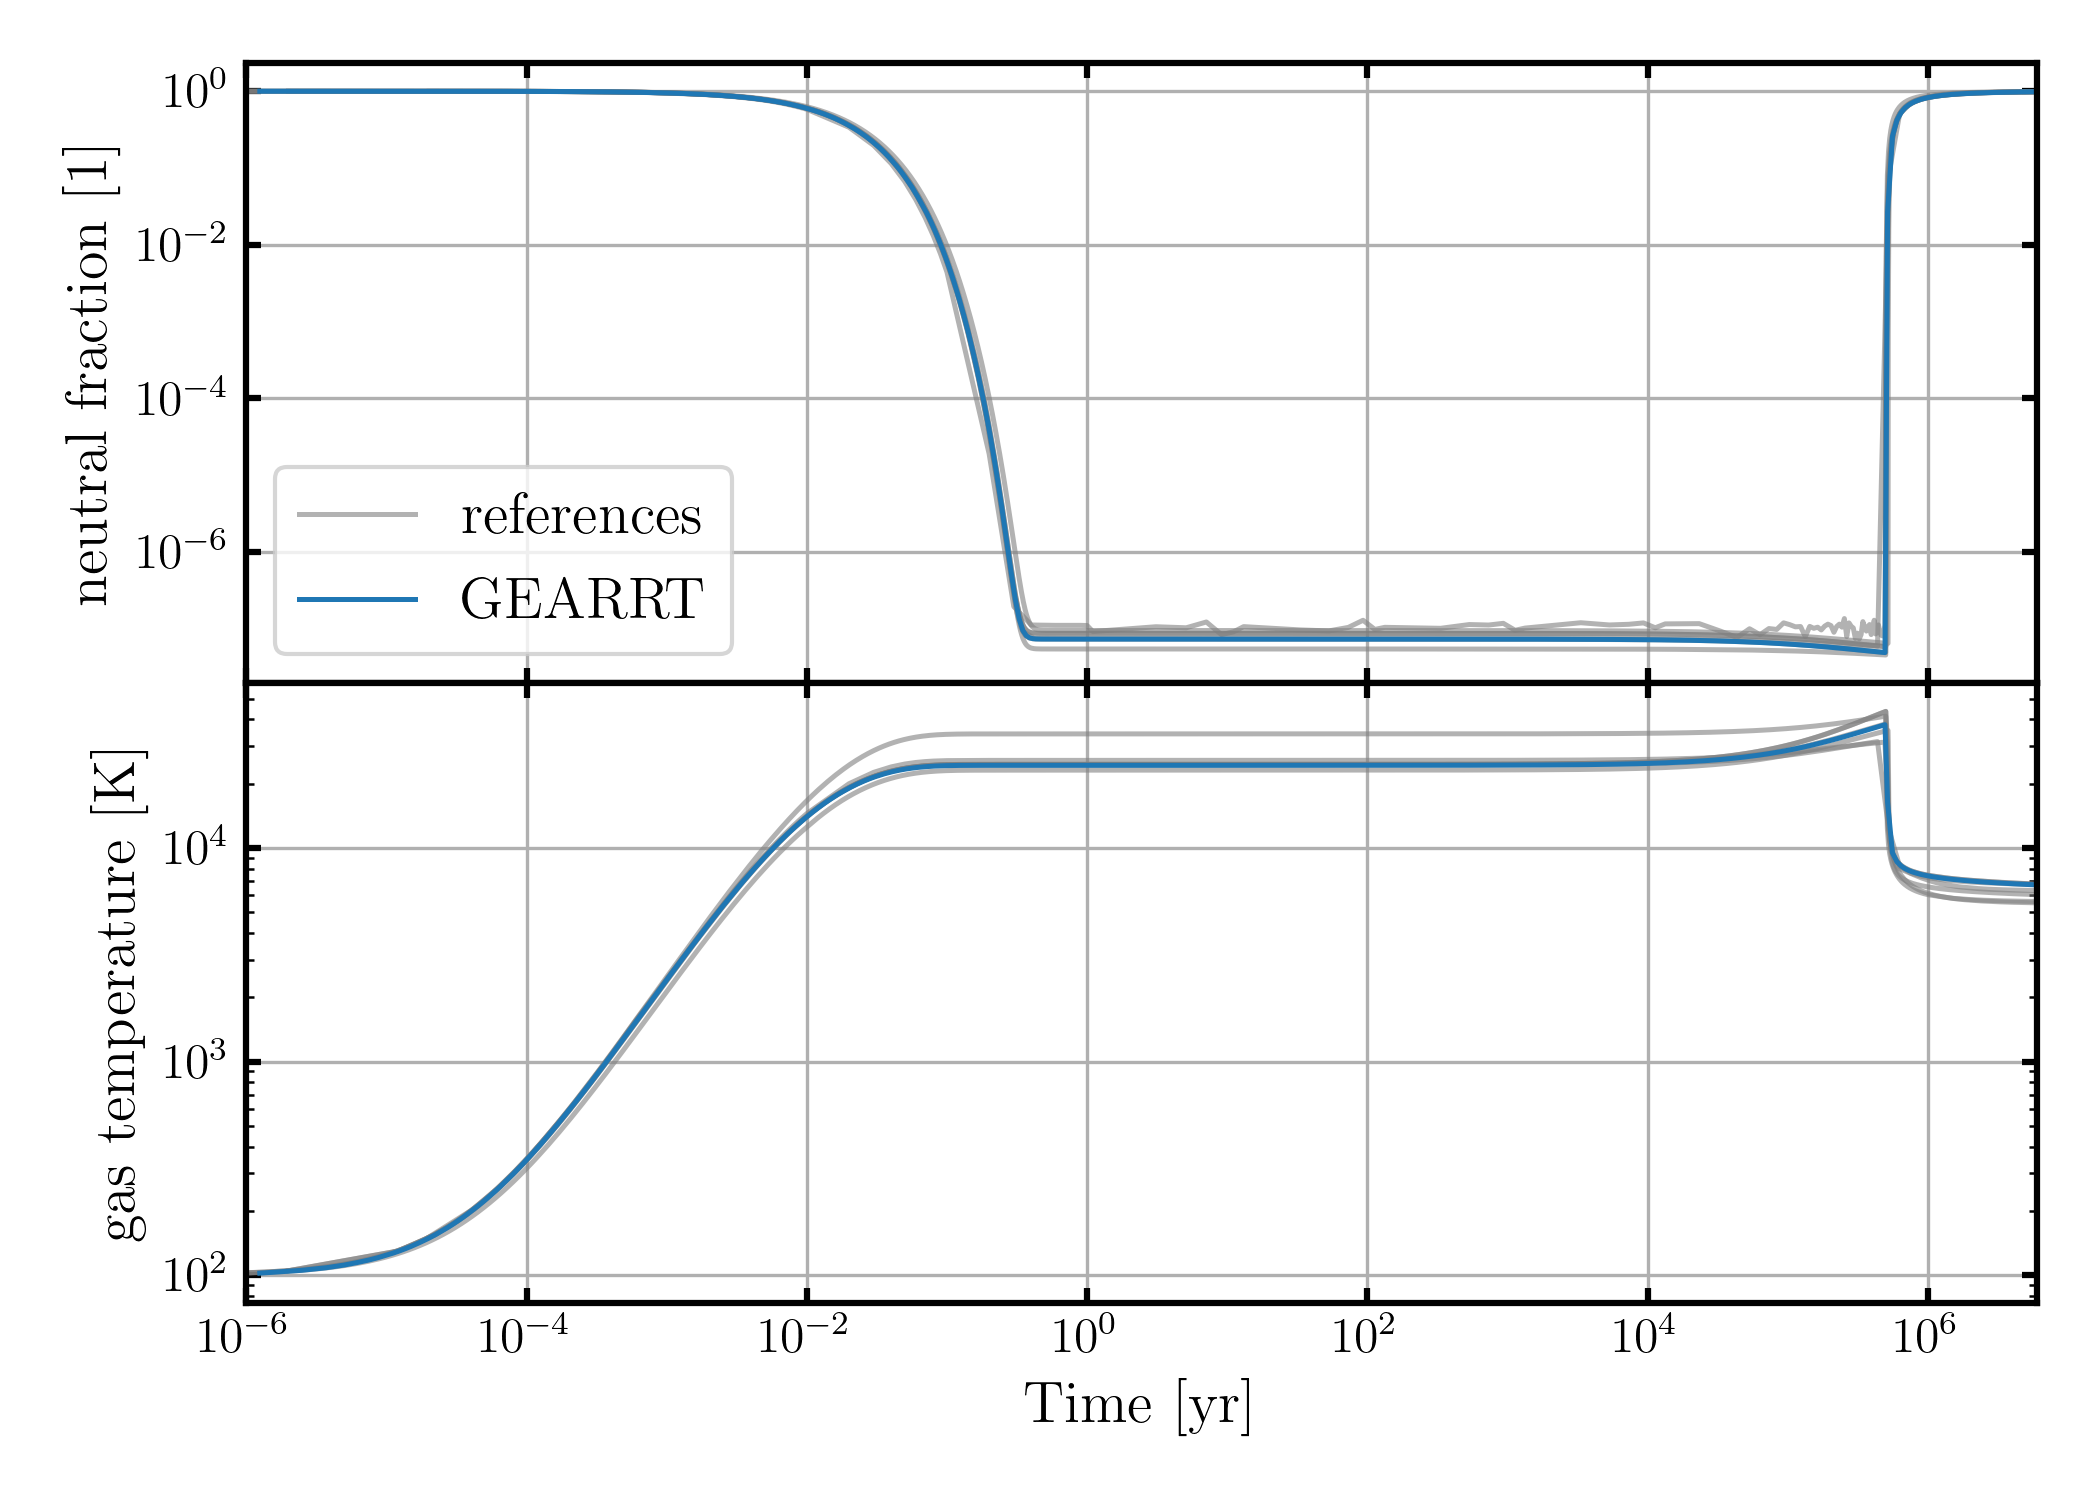
\includegraphics[width=\textwidth]{figures/RHD/ilievTest0part3.png}
 \caption{
 Test 0: Single zone photo-heating and ionization with subsequent cooling and recombination.
 }
 \label{fig:iliev0}
\end{figure}











%========================================================
\subsection{Iliev Test 1}\label{chap:Iliev1}
%========================================================




\begin{figure}
 \centering
 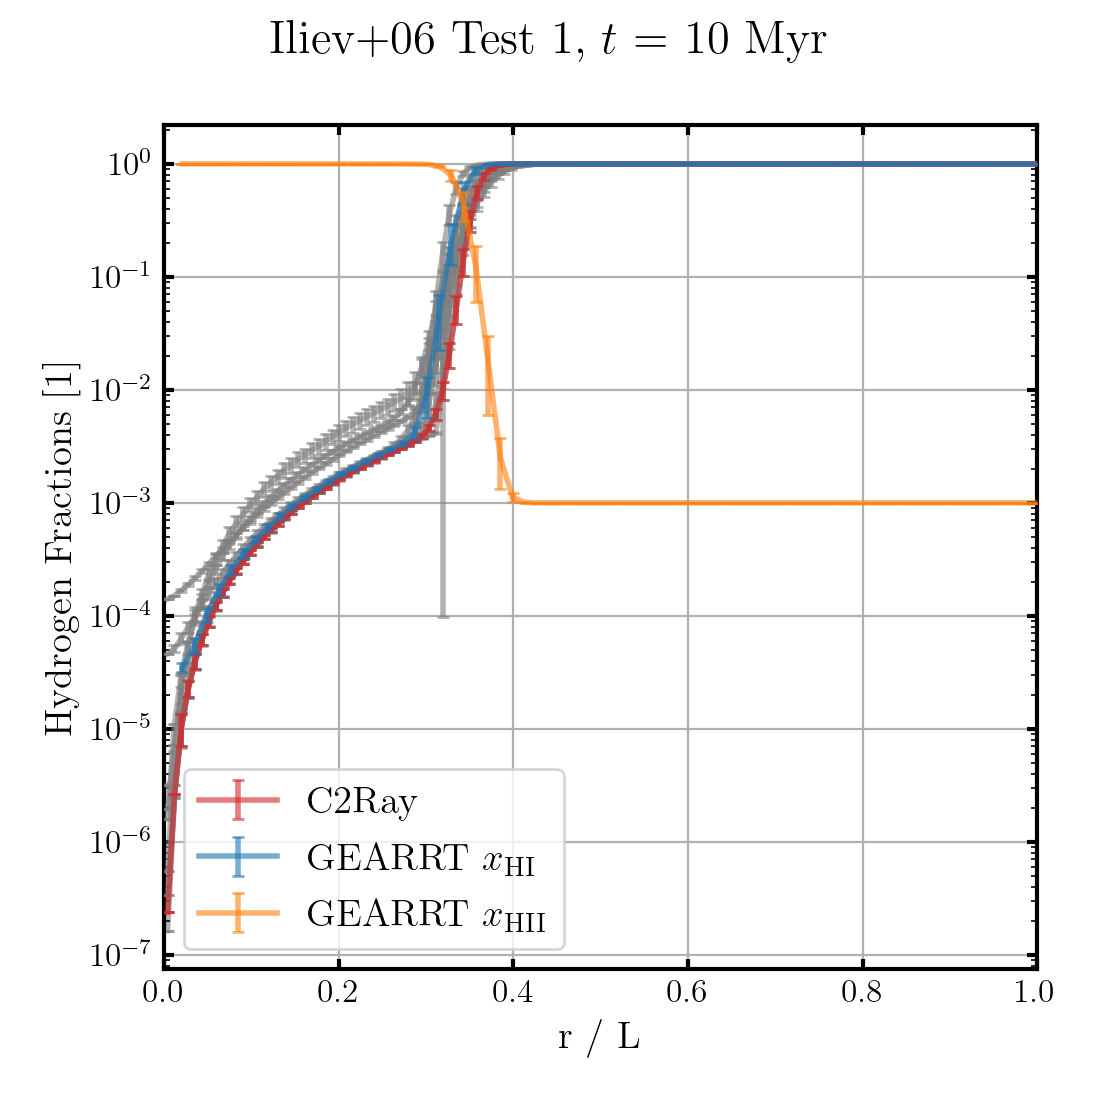
\includegraphics[width=.49\textwidth]{figures/RHD/Iliev1/output_0001.png}%
 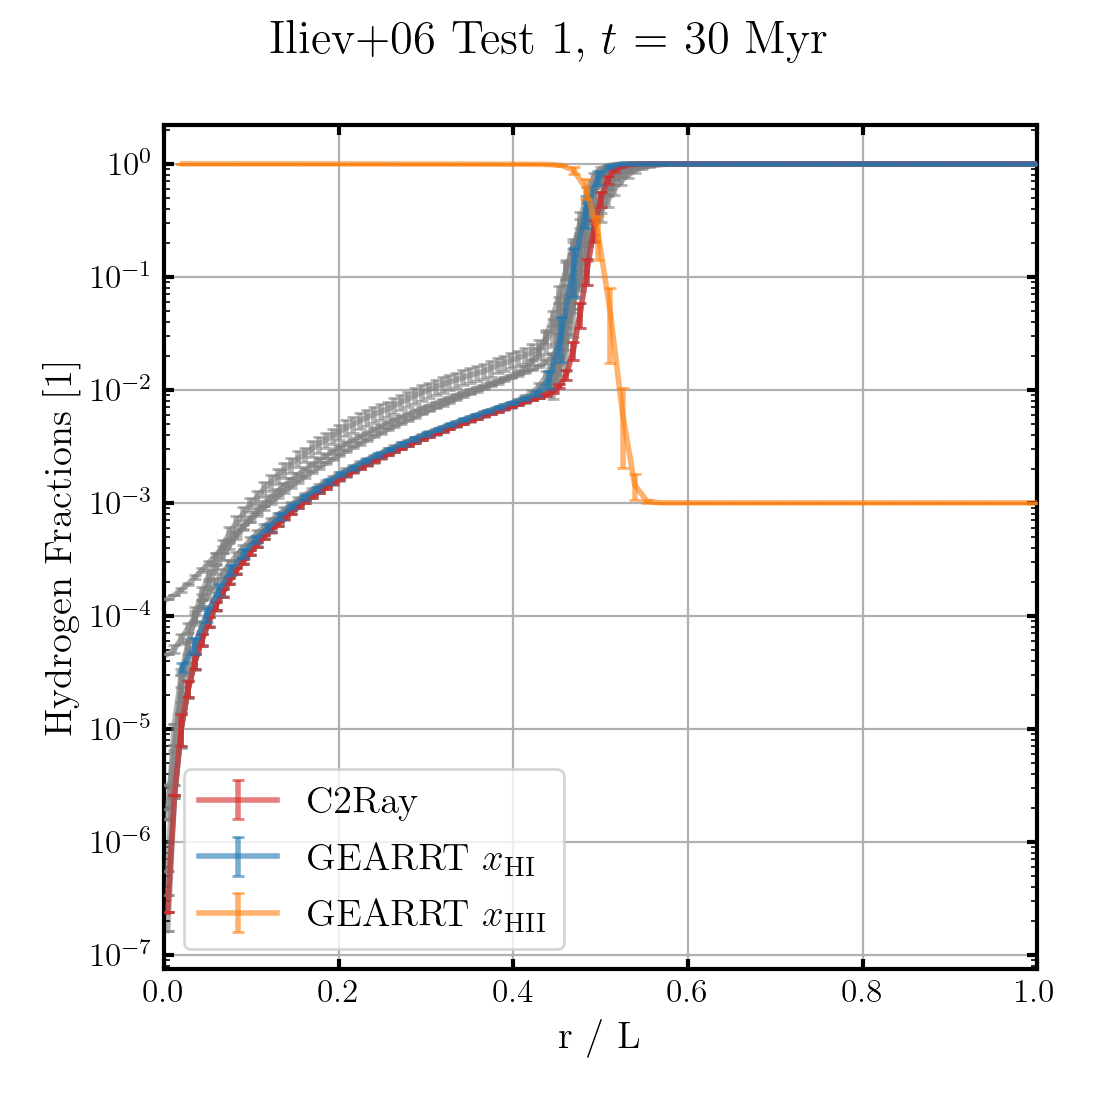
\includegraphics[width=.49\textwidth]{figures/RHD/Iliev1/output_0003.png}\\%
 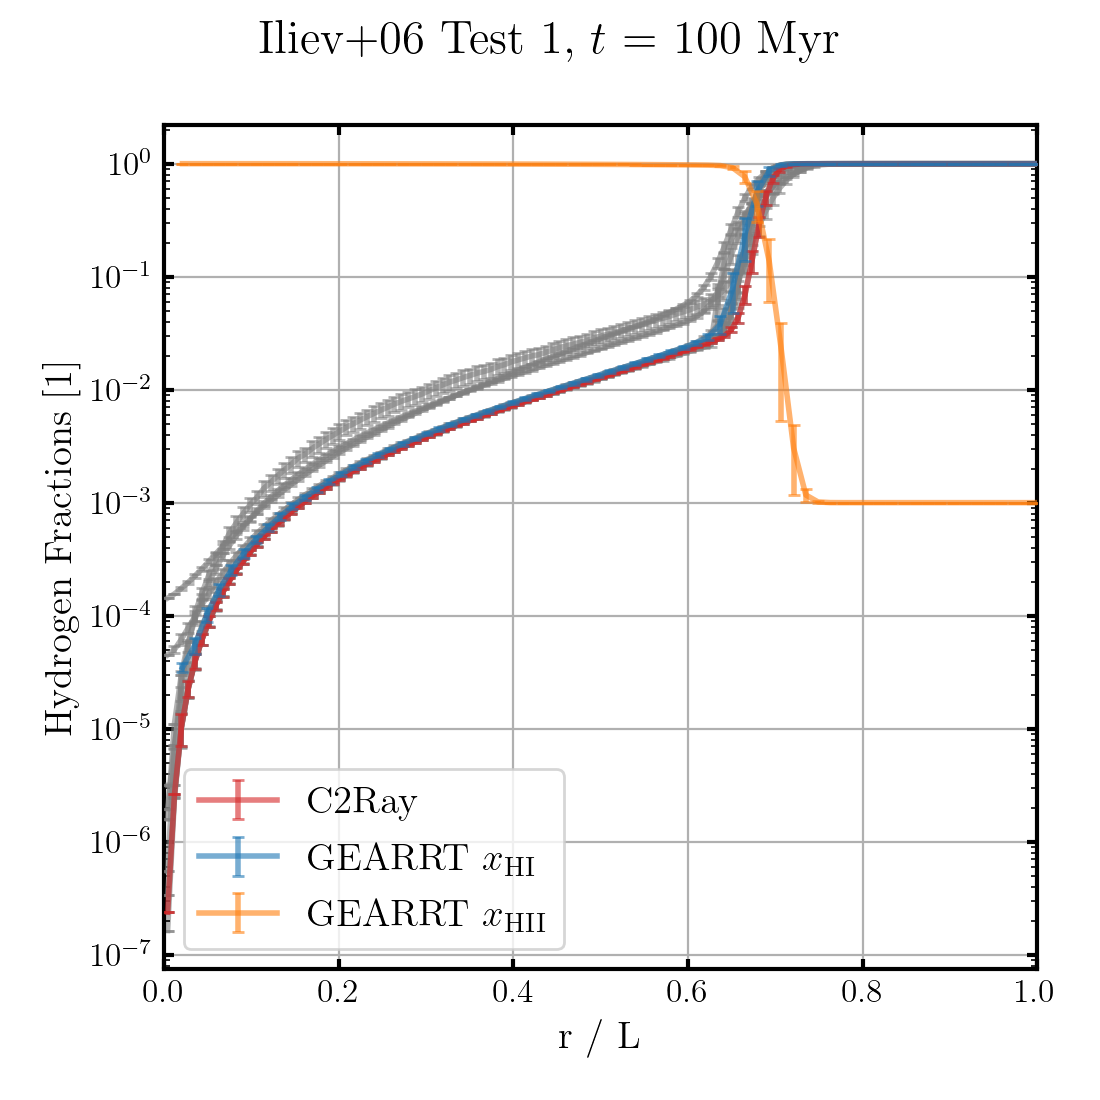
\includegraphics[width=.49\textwidth]{figures/RHD/Iliev1/output_0010.png}%
 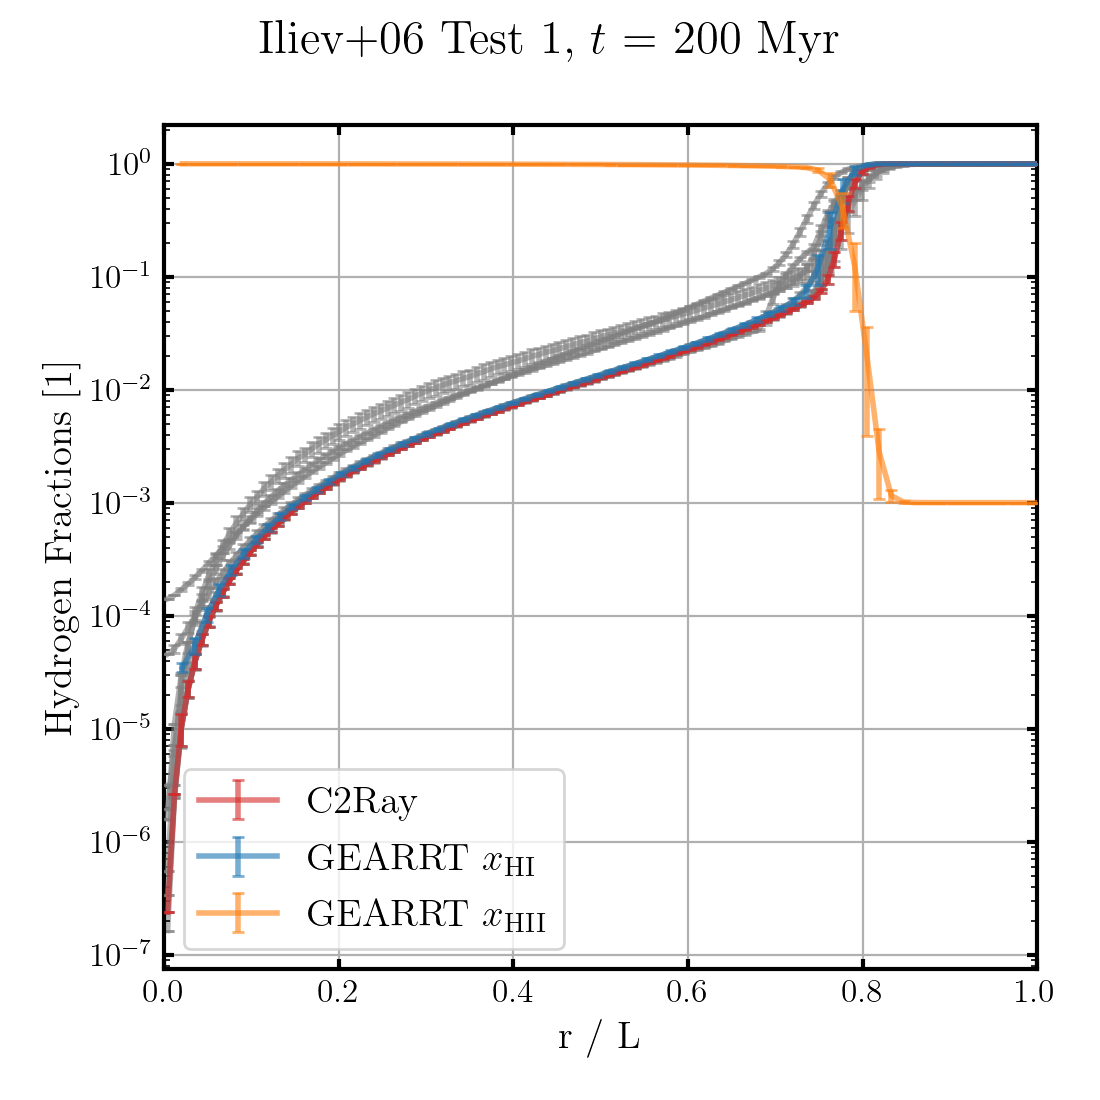
\includegraphics[width=.49\textwidth]{figures/RHD/Iliev1/output_0020.png}%
%  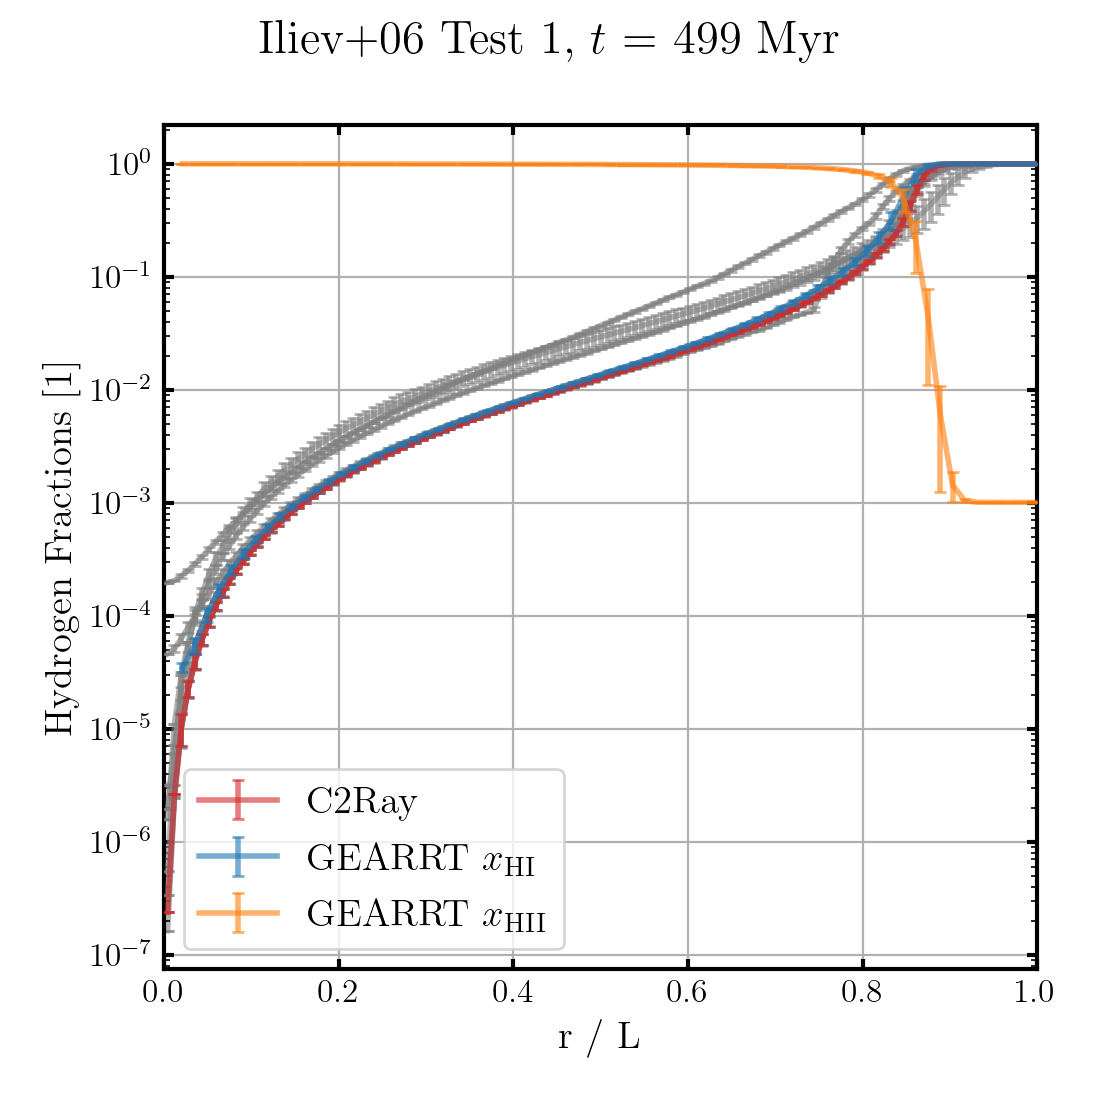
\includegraphics[width=.32\textwidth]{figures/RHD/Iliev1/output_0051.png}%
 \caption{
Spherically averaged ionized and neutral fractions of hydrogen in Test 1, where a single source
emits monochromatic ionizing radiation with frequency $h \nu = 13.6$eV at 10, 30, 100, and 200 Myr,
while the temperature is artificially held fixed at $T = 10^4$K. The error bars are standard
deviations.
 }
 \label{fig:iliev1}
\end{figure}


\begin{figure}
 \centering
 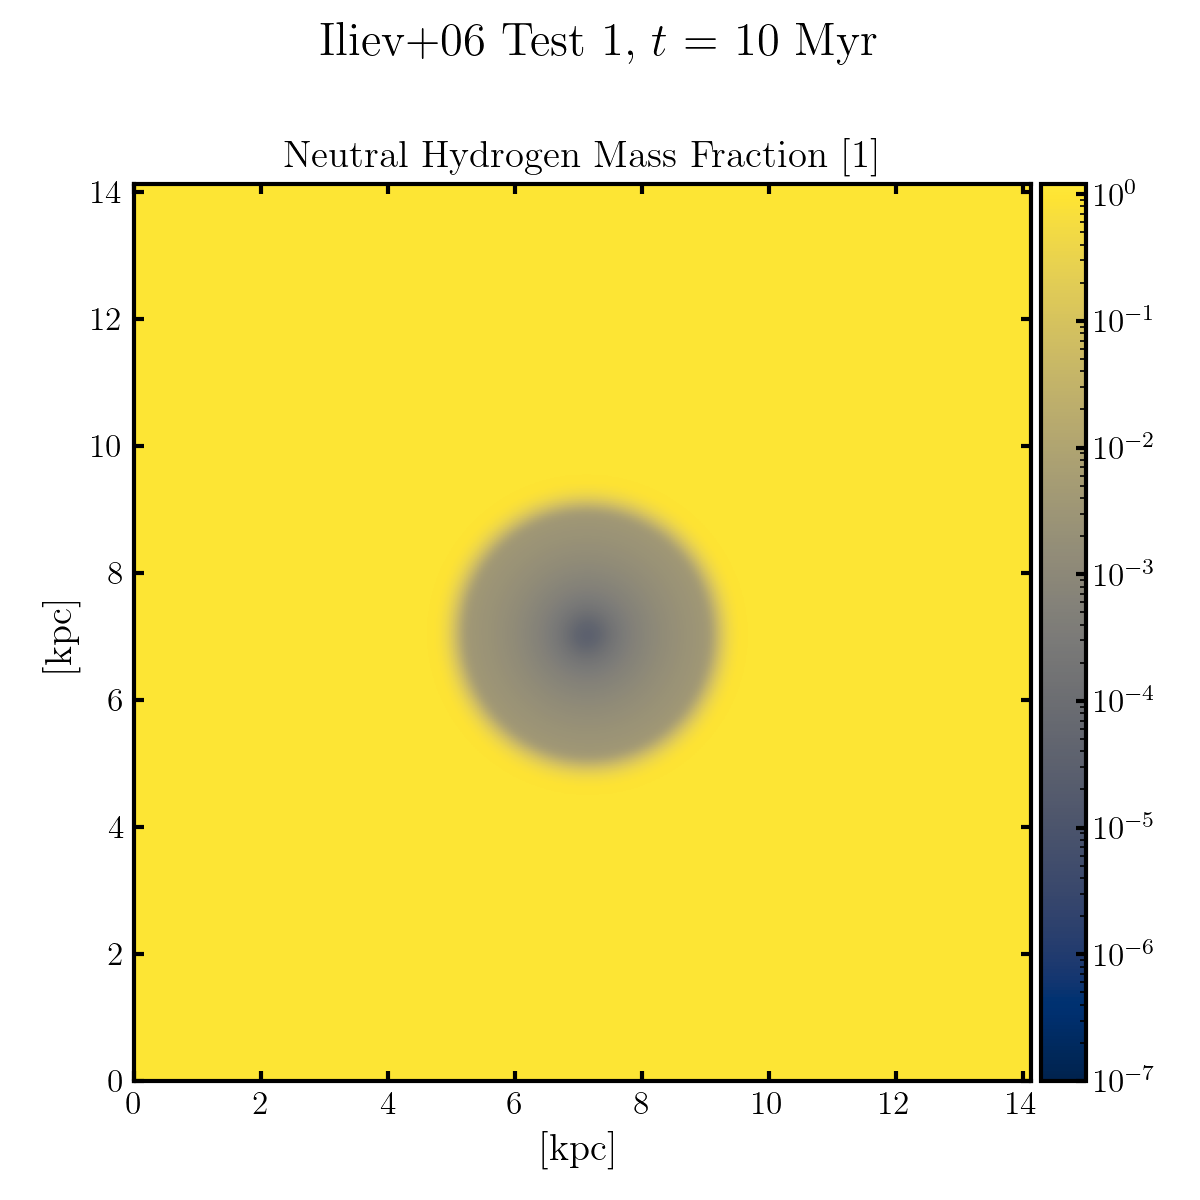
\includegraphics[width=.49\textwidth]{figures/RHD/Iliev1/output_0001-NoRef.png}%
 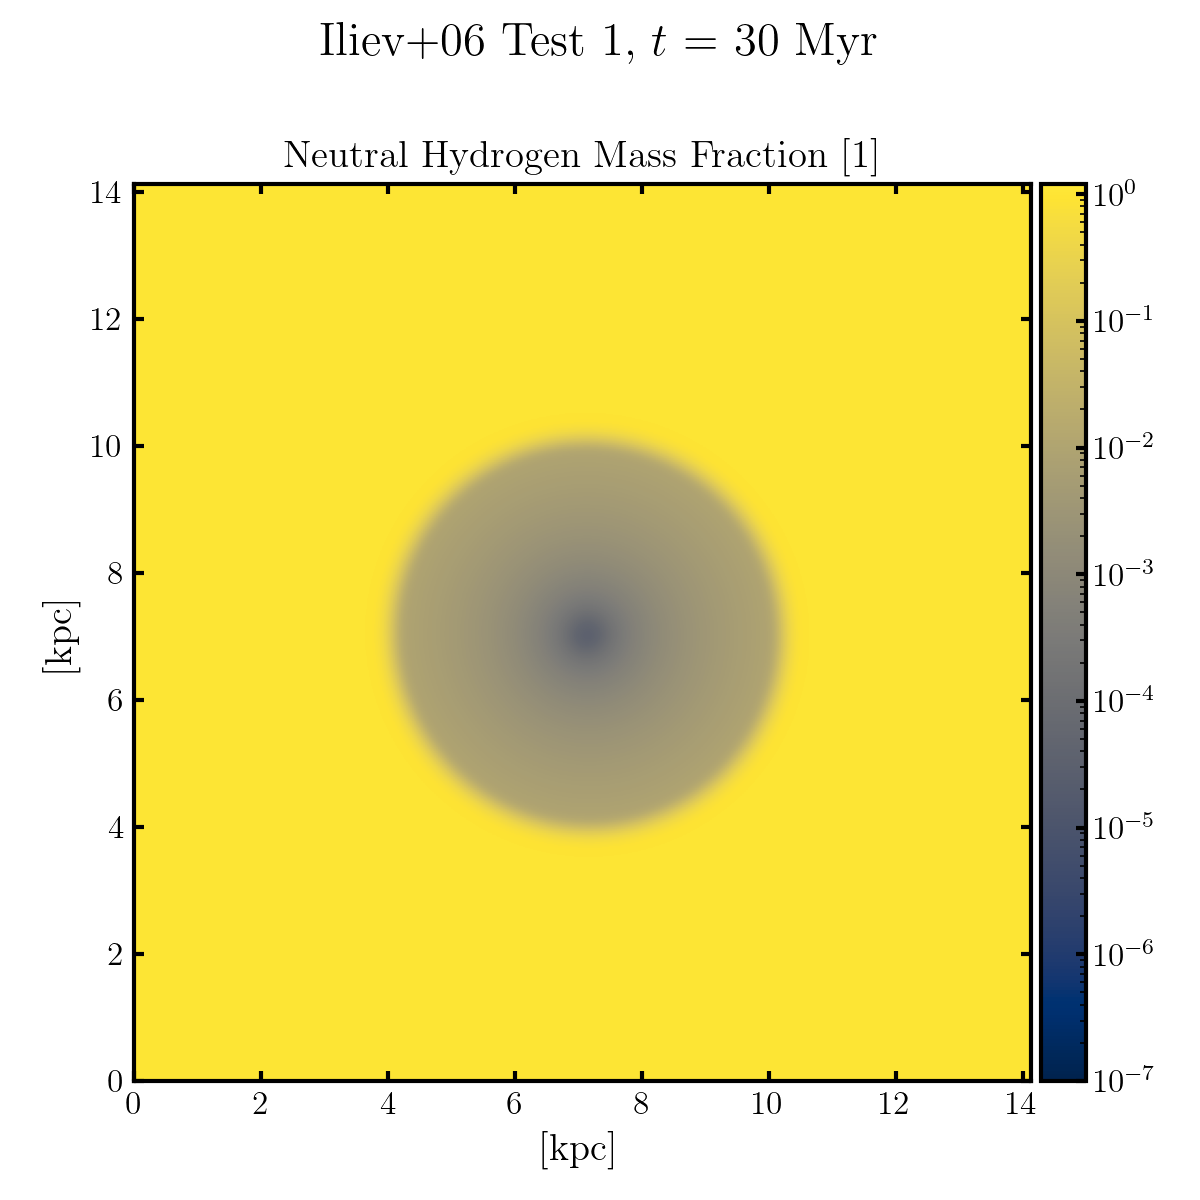
\includegraphics[width=.49\textwidth]{figures/RHD/Iliev1/output_0003-NoRef.png}\\%
 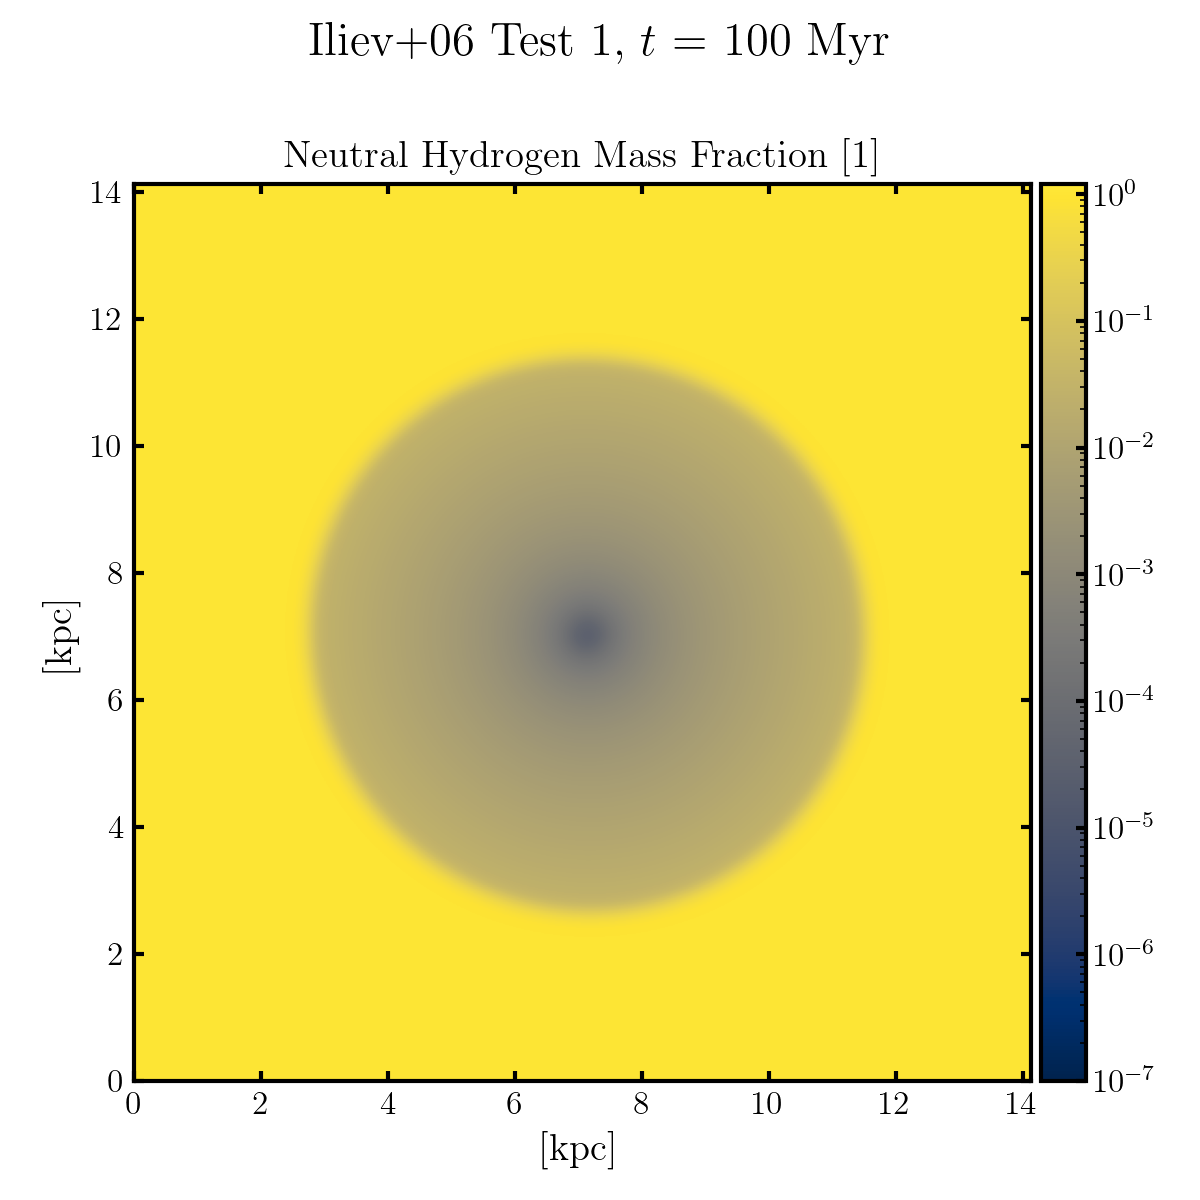
\includegraphics[width=.49\textwidth]{figures/RHD/Iliev1/output_0010-NoRef.png}%
 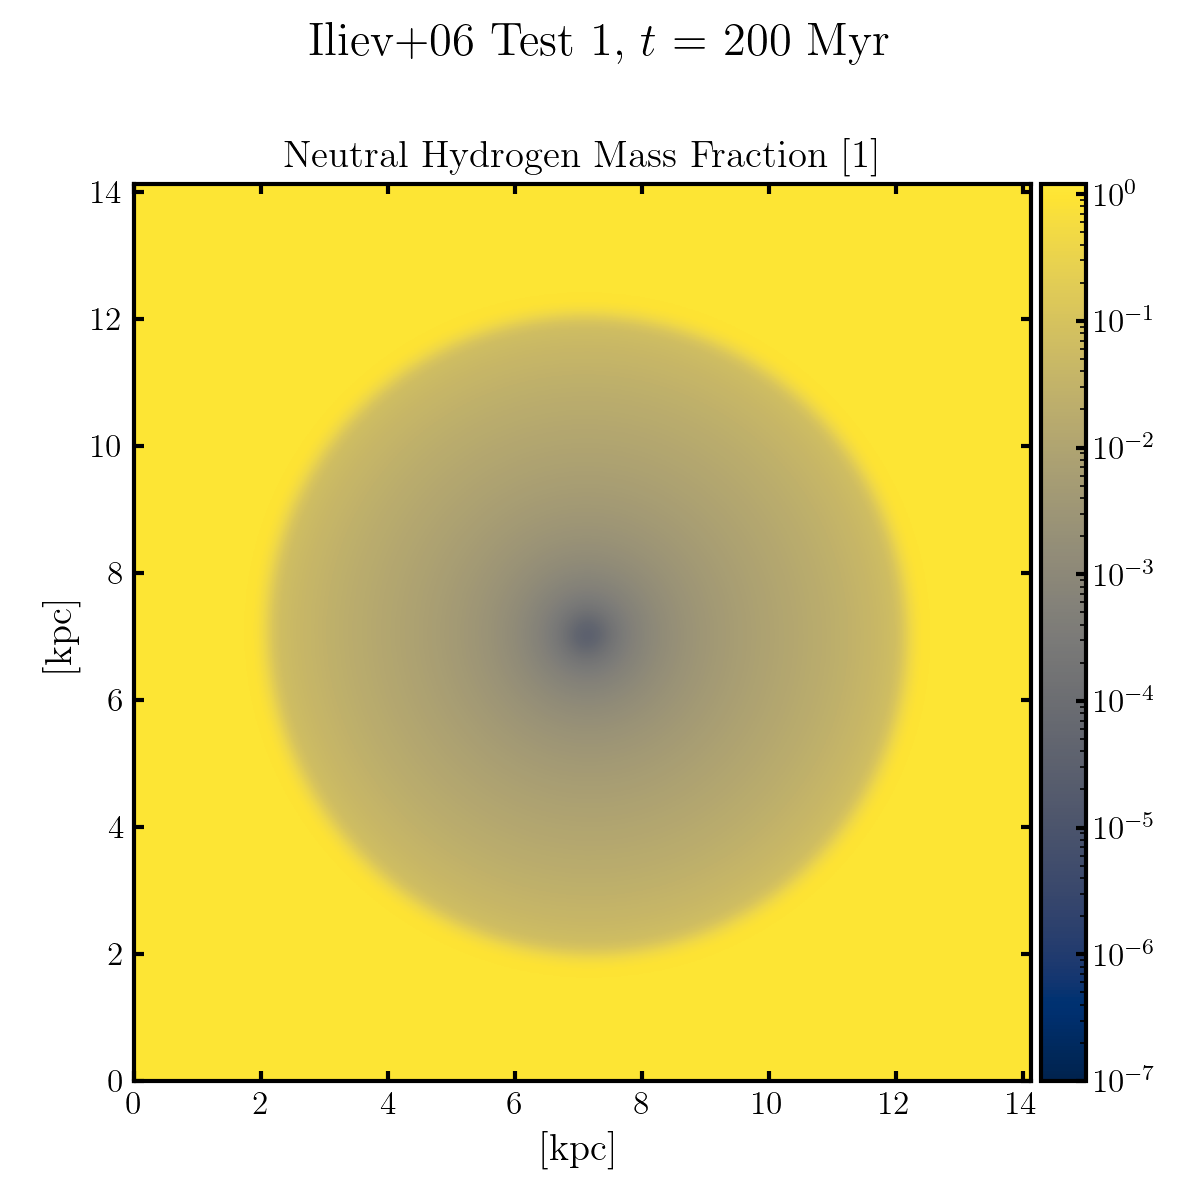
\includegraphics[width=.49\textwidth]{figures/RHD/Iliev1/output_0020-NoRef.png}%
%  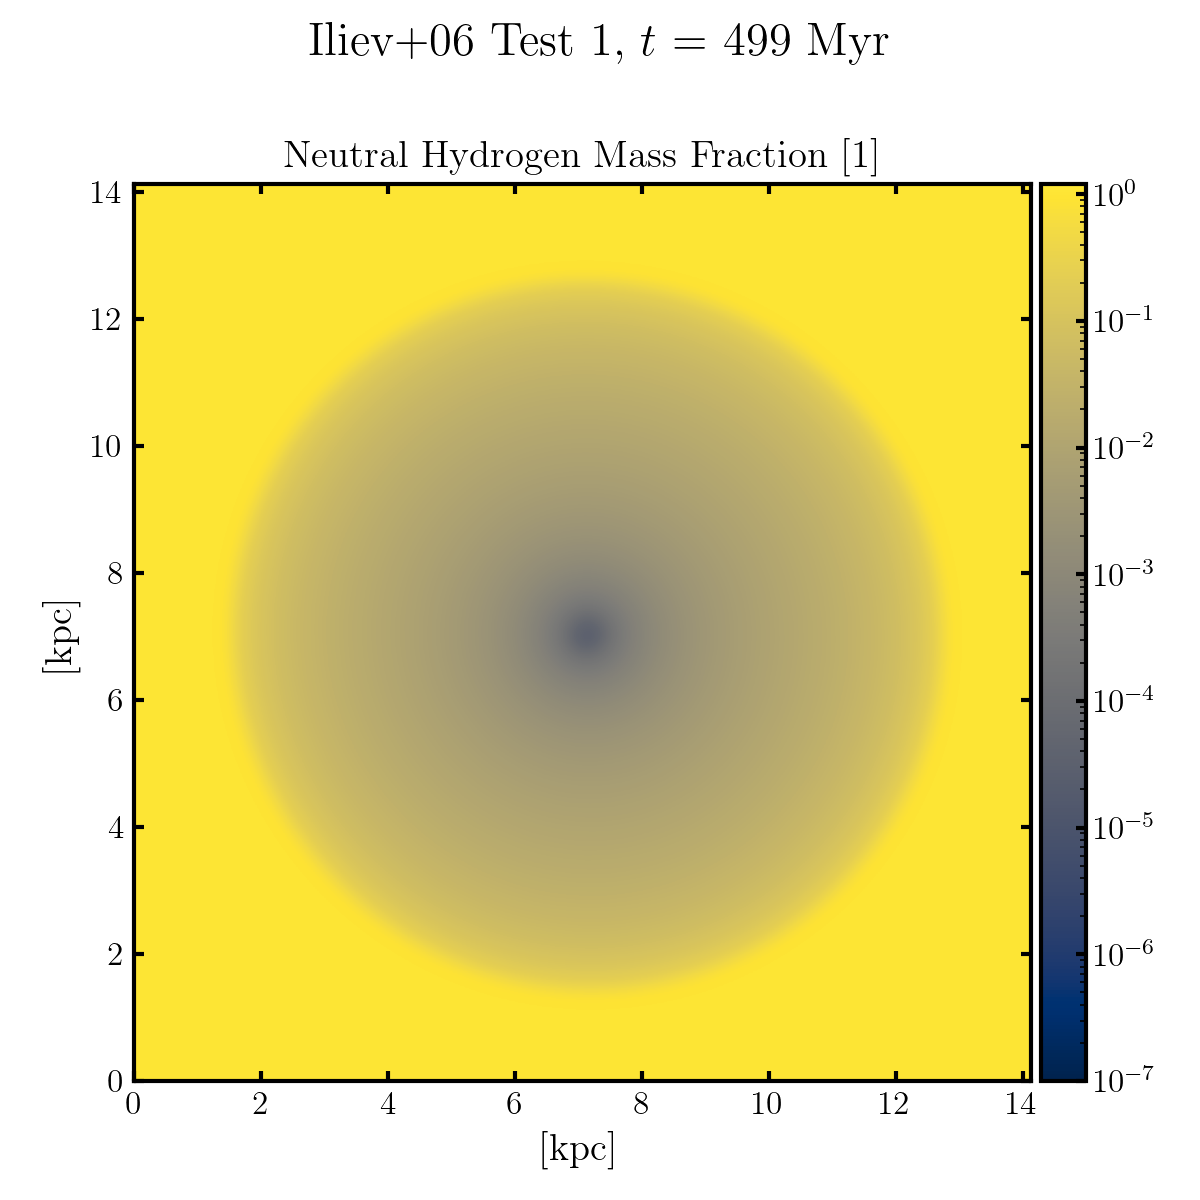
\includegraphics[width=.32\textwidth]{figures/RHD/Iliev1/output_0051-NoRef.png}%
 \caption{
Slices through the mid-plane of the box of the ionized hydrogen mass fraction in Test 1, where a
single source emits monochromatic ionizing radiation with frequency $h \nu = 13.6$eV at 10, 30, 100,
and 200 Myr.
 }
 \label{fig:iliev1-slices}
\end{figure}


\begin{figure}
 \centering
 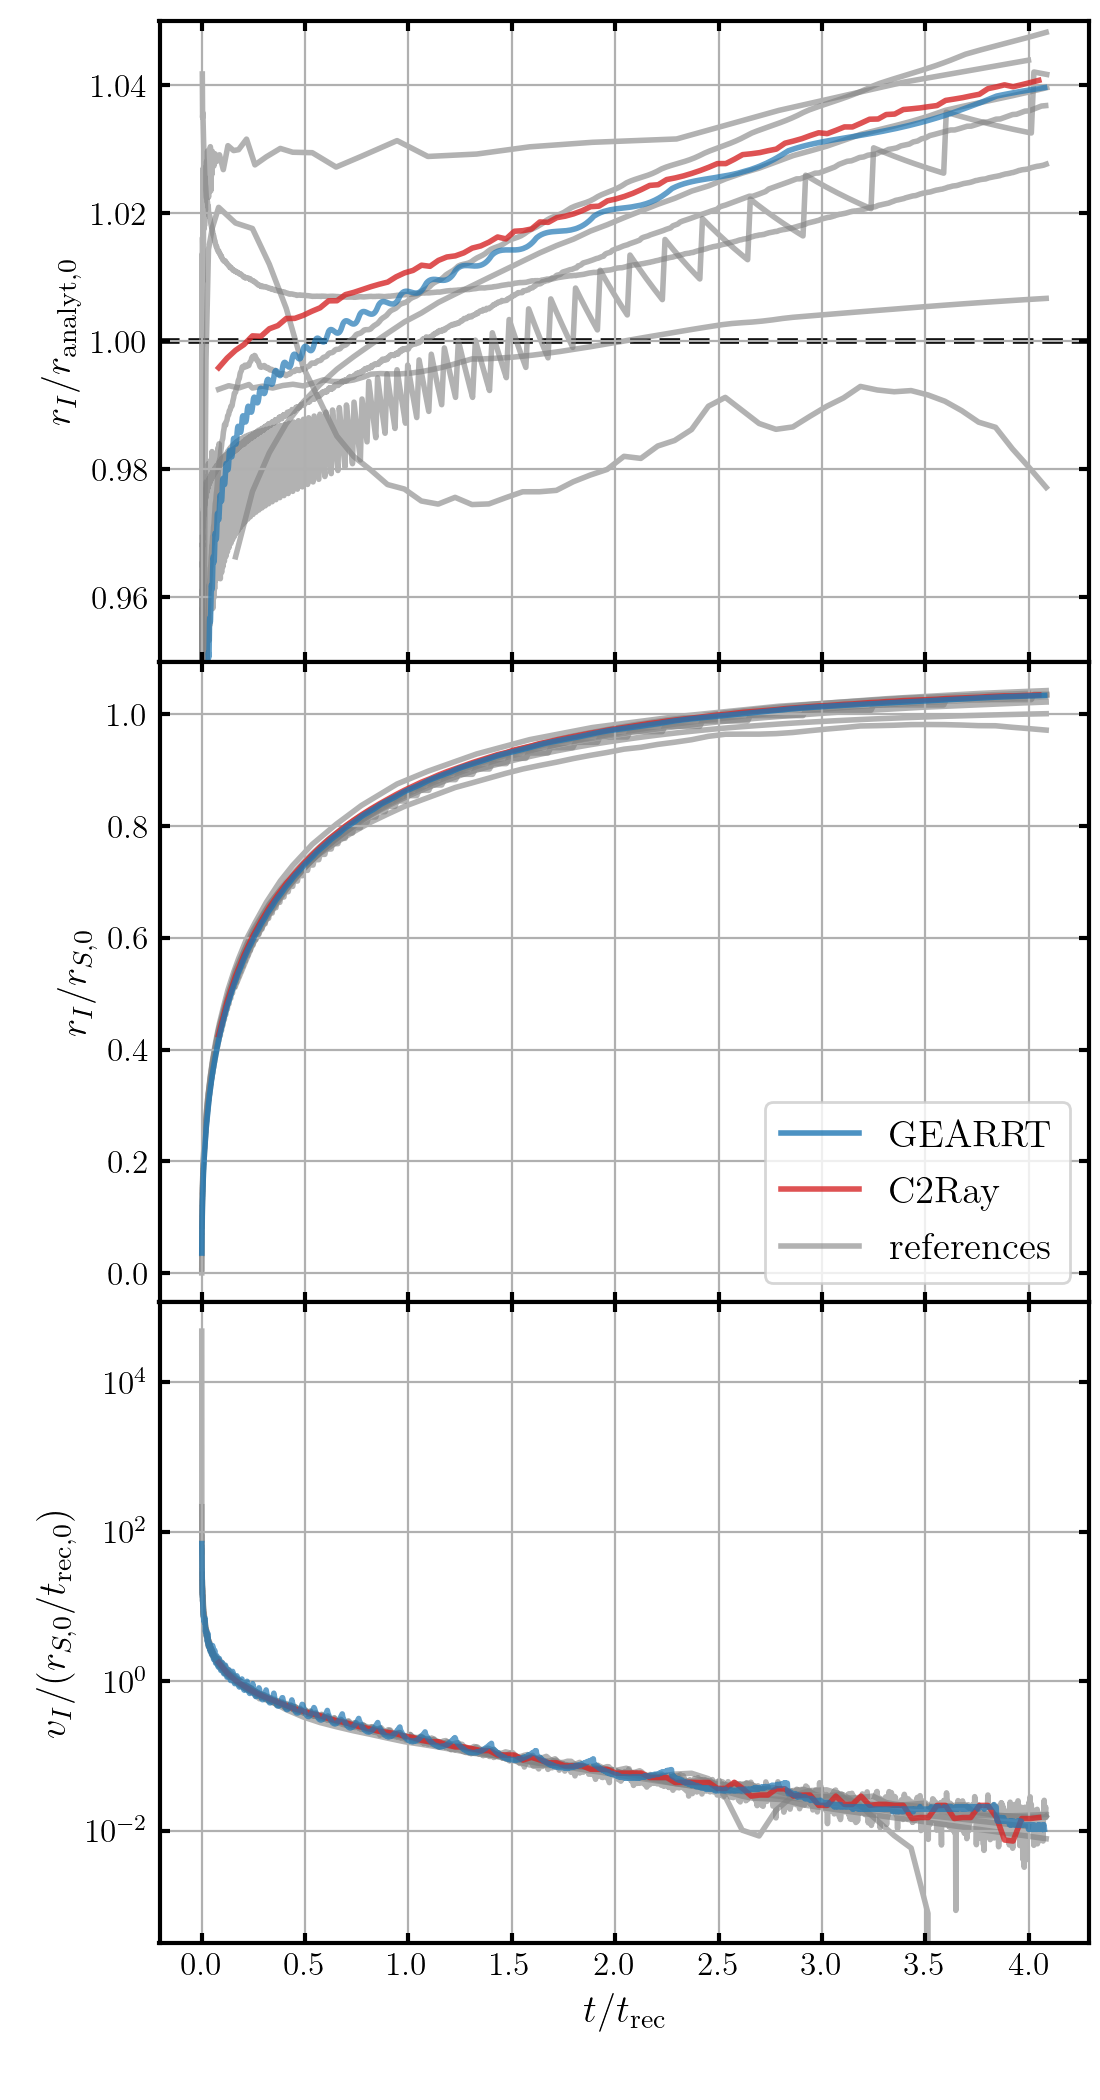
\includegraphics[width=.7\textwidth]{figures/RHD/Iliev1/ionization_fronts.png}%
 \caption{
 Evolution of the I-front position and velocity over time for Test 1.
 Top: Evolution of the I-front position over time, compared to the analytical position
(eq.~\ref{eq:rI}) and reference solutions from other codes.
 Middle: Evolution of the I-front position over time, compared to the final Str\"omgren radius
(eq.~\ref{eq:rS}).
 Bottom: Evolution of the I-front velocity.
 }
 \label{fig:iliev1-Ifront}
\end{figure}


Test 1 consists of a single source emitting monochromatic ($h\nu = 13.6$eV) radiation into an
initially neutral uniform hydrogen gas with number density $n = 10^{-3}$cm$^{-3}$. The temperature
of the gas is being kept constant at $T = 10^4$K throughout the entire simulation. The test in IL6
prescribe to put the ionizing source in the lower left corner of the simulation box, and to use
reflective boundary conditions along the three box sides adjacent to the source. However, in order
to avoid having to construct reflective boundary conditions for \GEARRT, which is not a trivial
matter with particles, I put the source in the center of the box, and make the box have twice the
size of what is prescribed in IL6, which results in a box size of $L = 13.2$ kpc. I use a glass file
consisting of $128^3$ particles for the particle positions of the uniform gas. IL6 use $128^3$
cells, but with half the box size compared to the one used here, so the results presented here will
be at half the spatial resolution compared to the results in IL6.\footnote{
While in principle it would be possible to run the tests at the same resolution as in IL6, the
results obtained with the reduced resolution are perfectly sufficient to demonstrate the validity of
\GEARRT, and I opted to avoid the otherwise increased computational load of a factor of eight.}
The ionizing photon rate emitted by the source is $\dot{N}_\gamma = 5 \times 10^{48}$ photons/s. I
reduce the speed of light by a factor of 100. (The validity of this value for the reduced speed of
light will be verified in Test 2).

The expected solution should be an expanding HII region, known as a Str\"omgren sphere. Assuming
the ionization front (I-front) is infinitely sharp, the I-front radius has an analytical solution
given by

\begin{align}
    r_I = r_S ( 1 - \exp(-t/t_{rec}))^{1/3} \label{eq:rI}
\end{align}

and its velocity is

\begin{align}
    v_I = \deldt{r_I} = \frac{r_S}{3 t_{rec}} \frac{\exp(-t/t_{rec})}{( 1 -
\exp(-t/t_{rec}))^{2/3}} \label{eq:vI}
\end{align}

where

\begin{align}
    r_S &= \left[ \frac{3 \dot{N}_\gamma}{4 \pi \alpha(T) n_H^2} \right]^{1/3} \label{eq:rS} \\
    t_{rec} &= \frac{1}{\alpha_B(T) n_H}
\end{align}

are the Str\"omgren radius and the recombination time, respectively.
$\alpha_B(T)$ is the Case B recombination rate of hydrogen. For $T = 10^4$K, $\alpha_B =
2.59 \times 10^{-13}$cm$^3/$s and $\dot{N_\gamma} = 5 \times 10^{48}$ photons/s, we have $r_S =
5.4$ kpc and $t_{rec} = 122.4$ Myr.

Figure~\ref{fig:iliev1} shows the spherically averaged profiles of neutral fractions of hydrogen at
10, 30, 100, and 200 Myr, while Figure~\ref{fig:iliev1-slices} shows the slices through the
mid-plane of the box at the same output times. \GEARRT shows again good agreement with the reference
solutions. The position of the I-front radius, defined as the radius at which the ion mass fraction
is exactly 0.5, and velocity is shown in Figure~\ref{fig:iliev1-Ifront}, and also agrees well with
the reference solutions. At early times ($t \lesssim t_{rec}$) the ionization front radius lags a
little behind compared to the results of \codename{C2Ray}, which is due to the reduced speed of
light used by \GEARRT. At later times, the I-front radius is ahead of the analytical solution for
most reference codes as well as for \GEARRT due to the assumption of a sharp I-front used to derive
the analytical solution. More precisely, the analytical solution assumed that the I-front is a sharp
discontinuity, and that the HII region is fully ionized, which is not exactly the case.
Indeed \citet{pawlikTRAPHICRadiativeTransfer2008} have derived that the analytical equilibrium
solution for the position of the I-front defined as the radius at which the ionization is exactly
half results in 1.05$r_S$, which is in good agreement with the results by \GEARRT and other codes
shown in Figure~\ref{fig:iliev1-Ifront}. In order to reproduce figures close to those presented in
IL6 and \citet{ramses-rt13}, I chose to keep the reference values as specified by IL6.









%========================================================
\subsection{Iliev Test 2}\label{chap:Iliev2}
%========================================================



\begin{figure}
 \centering
 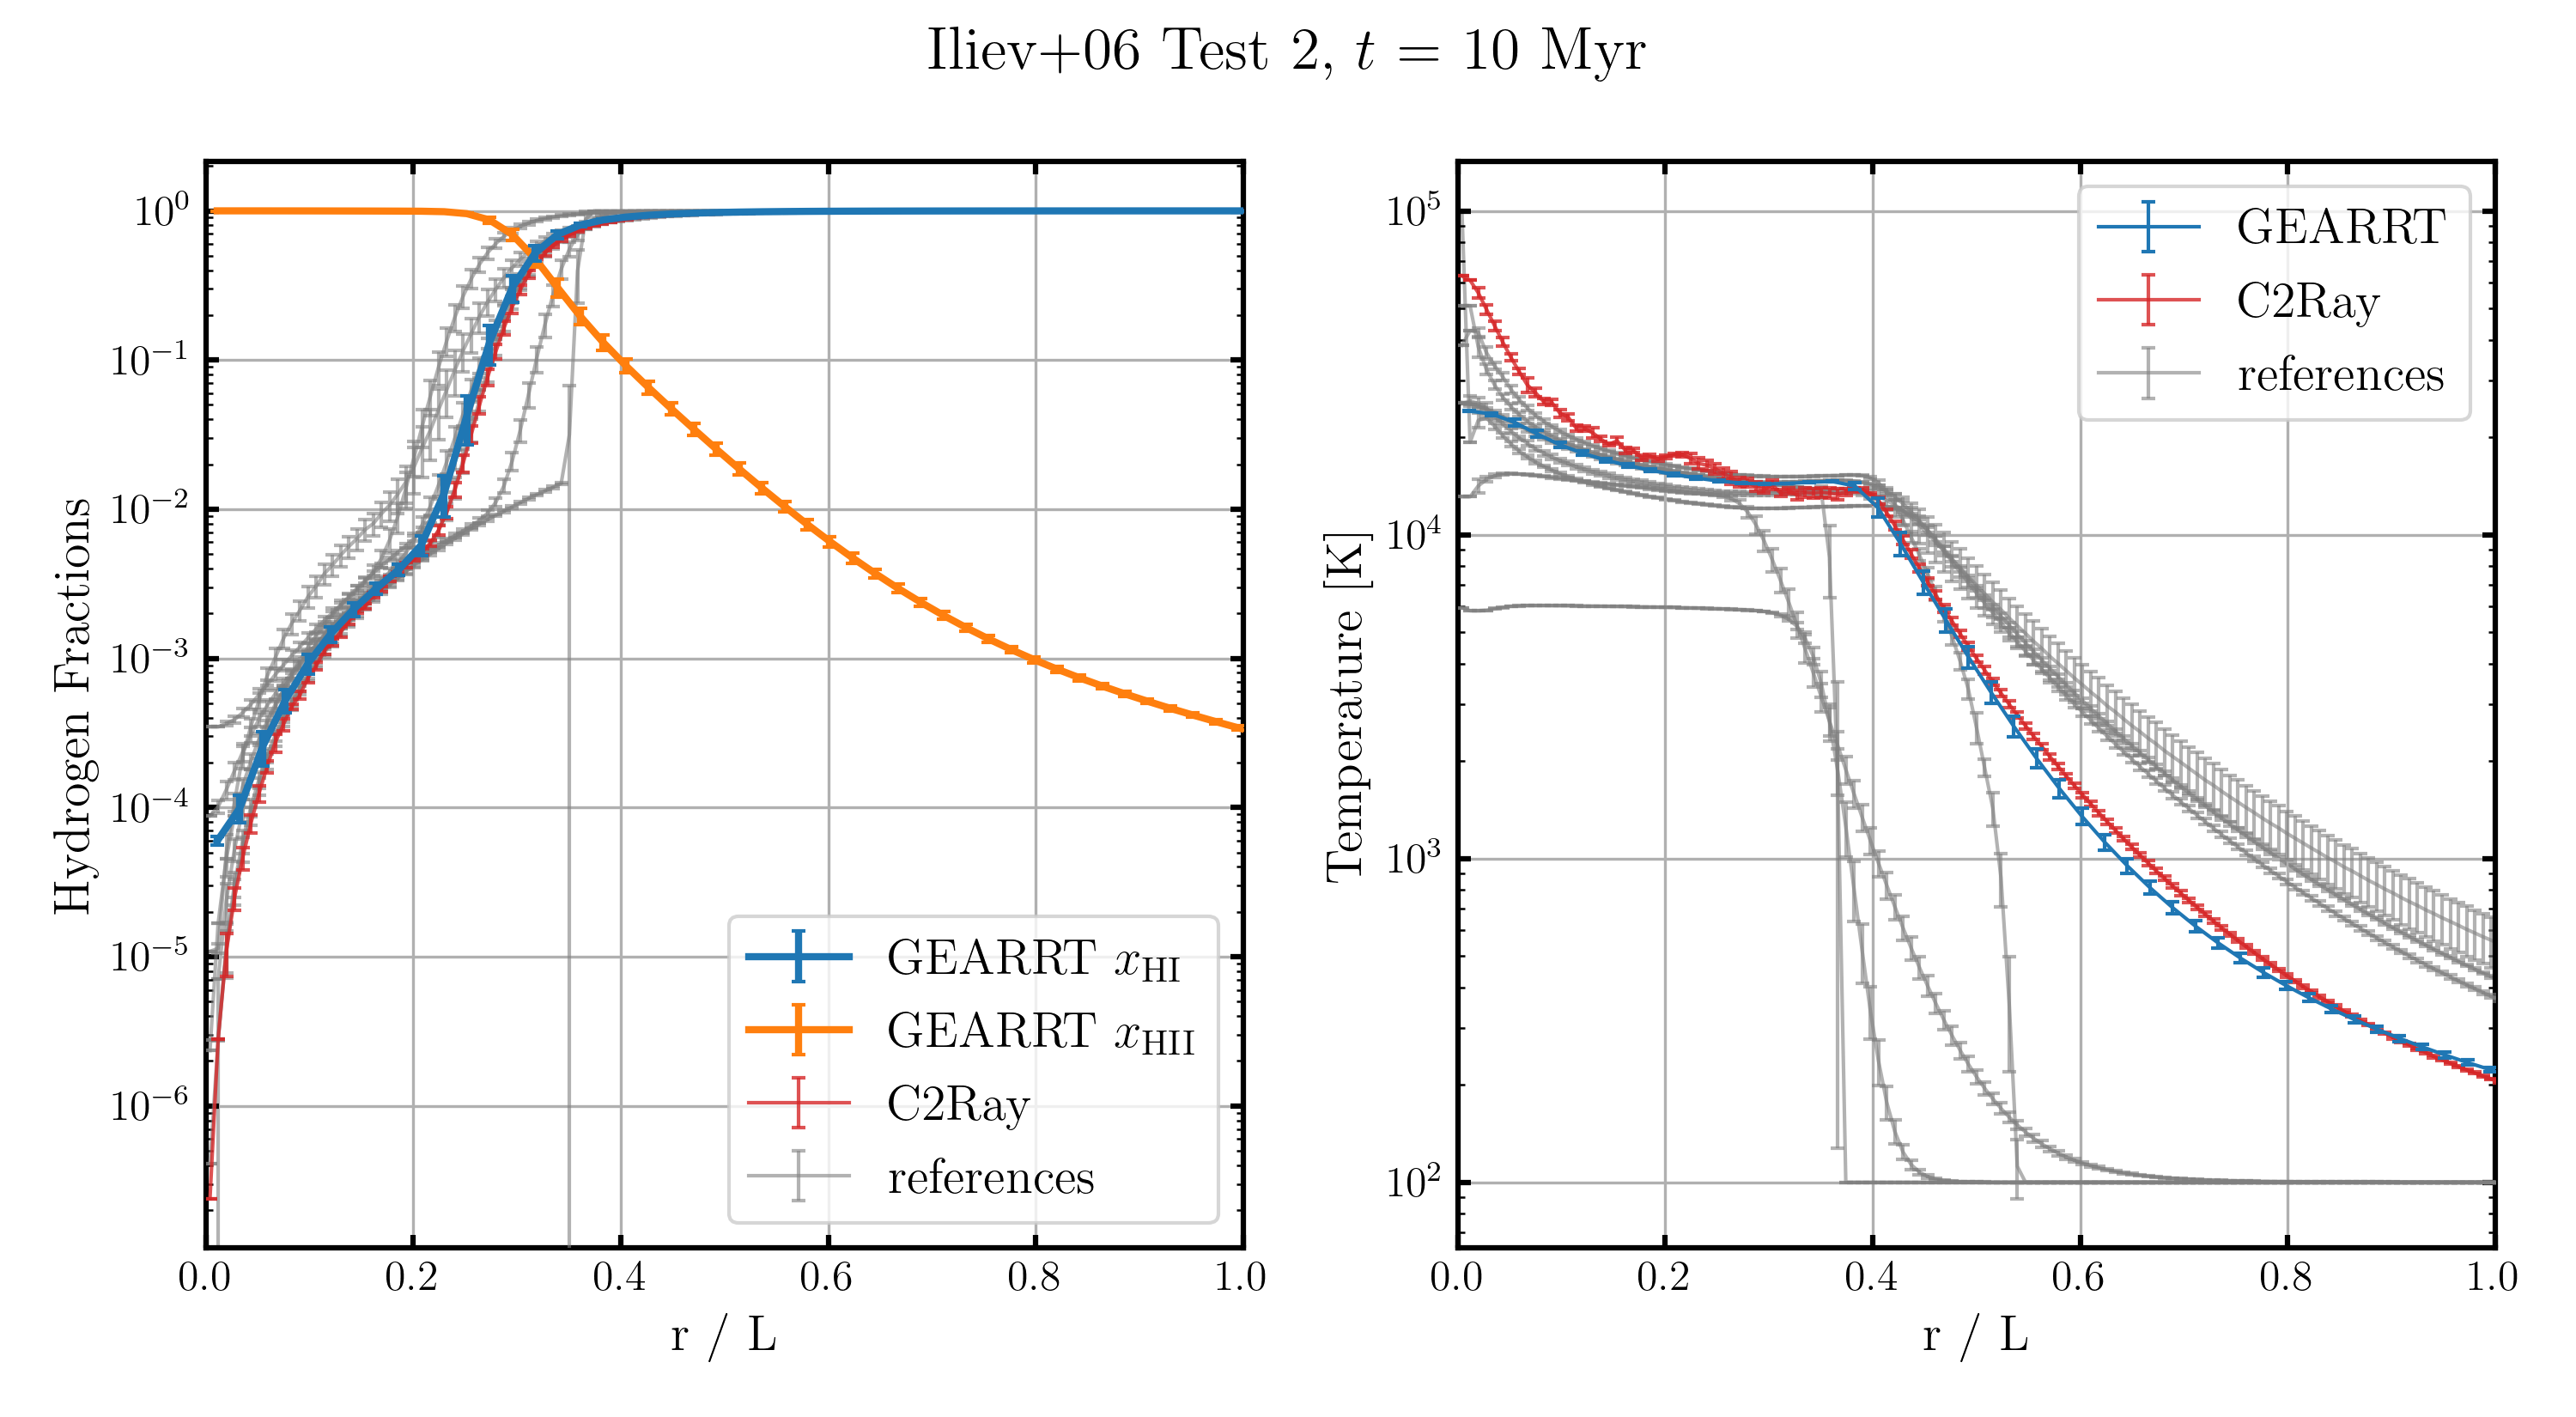
\includegraphics[width=.85\textwidth]{figures/RHD/Iliev2/output_0001.png}\\%
 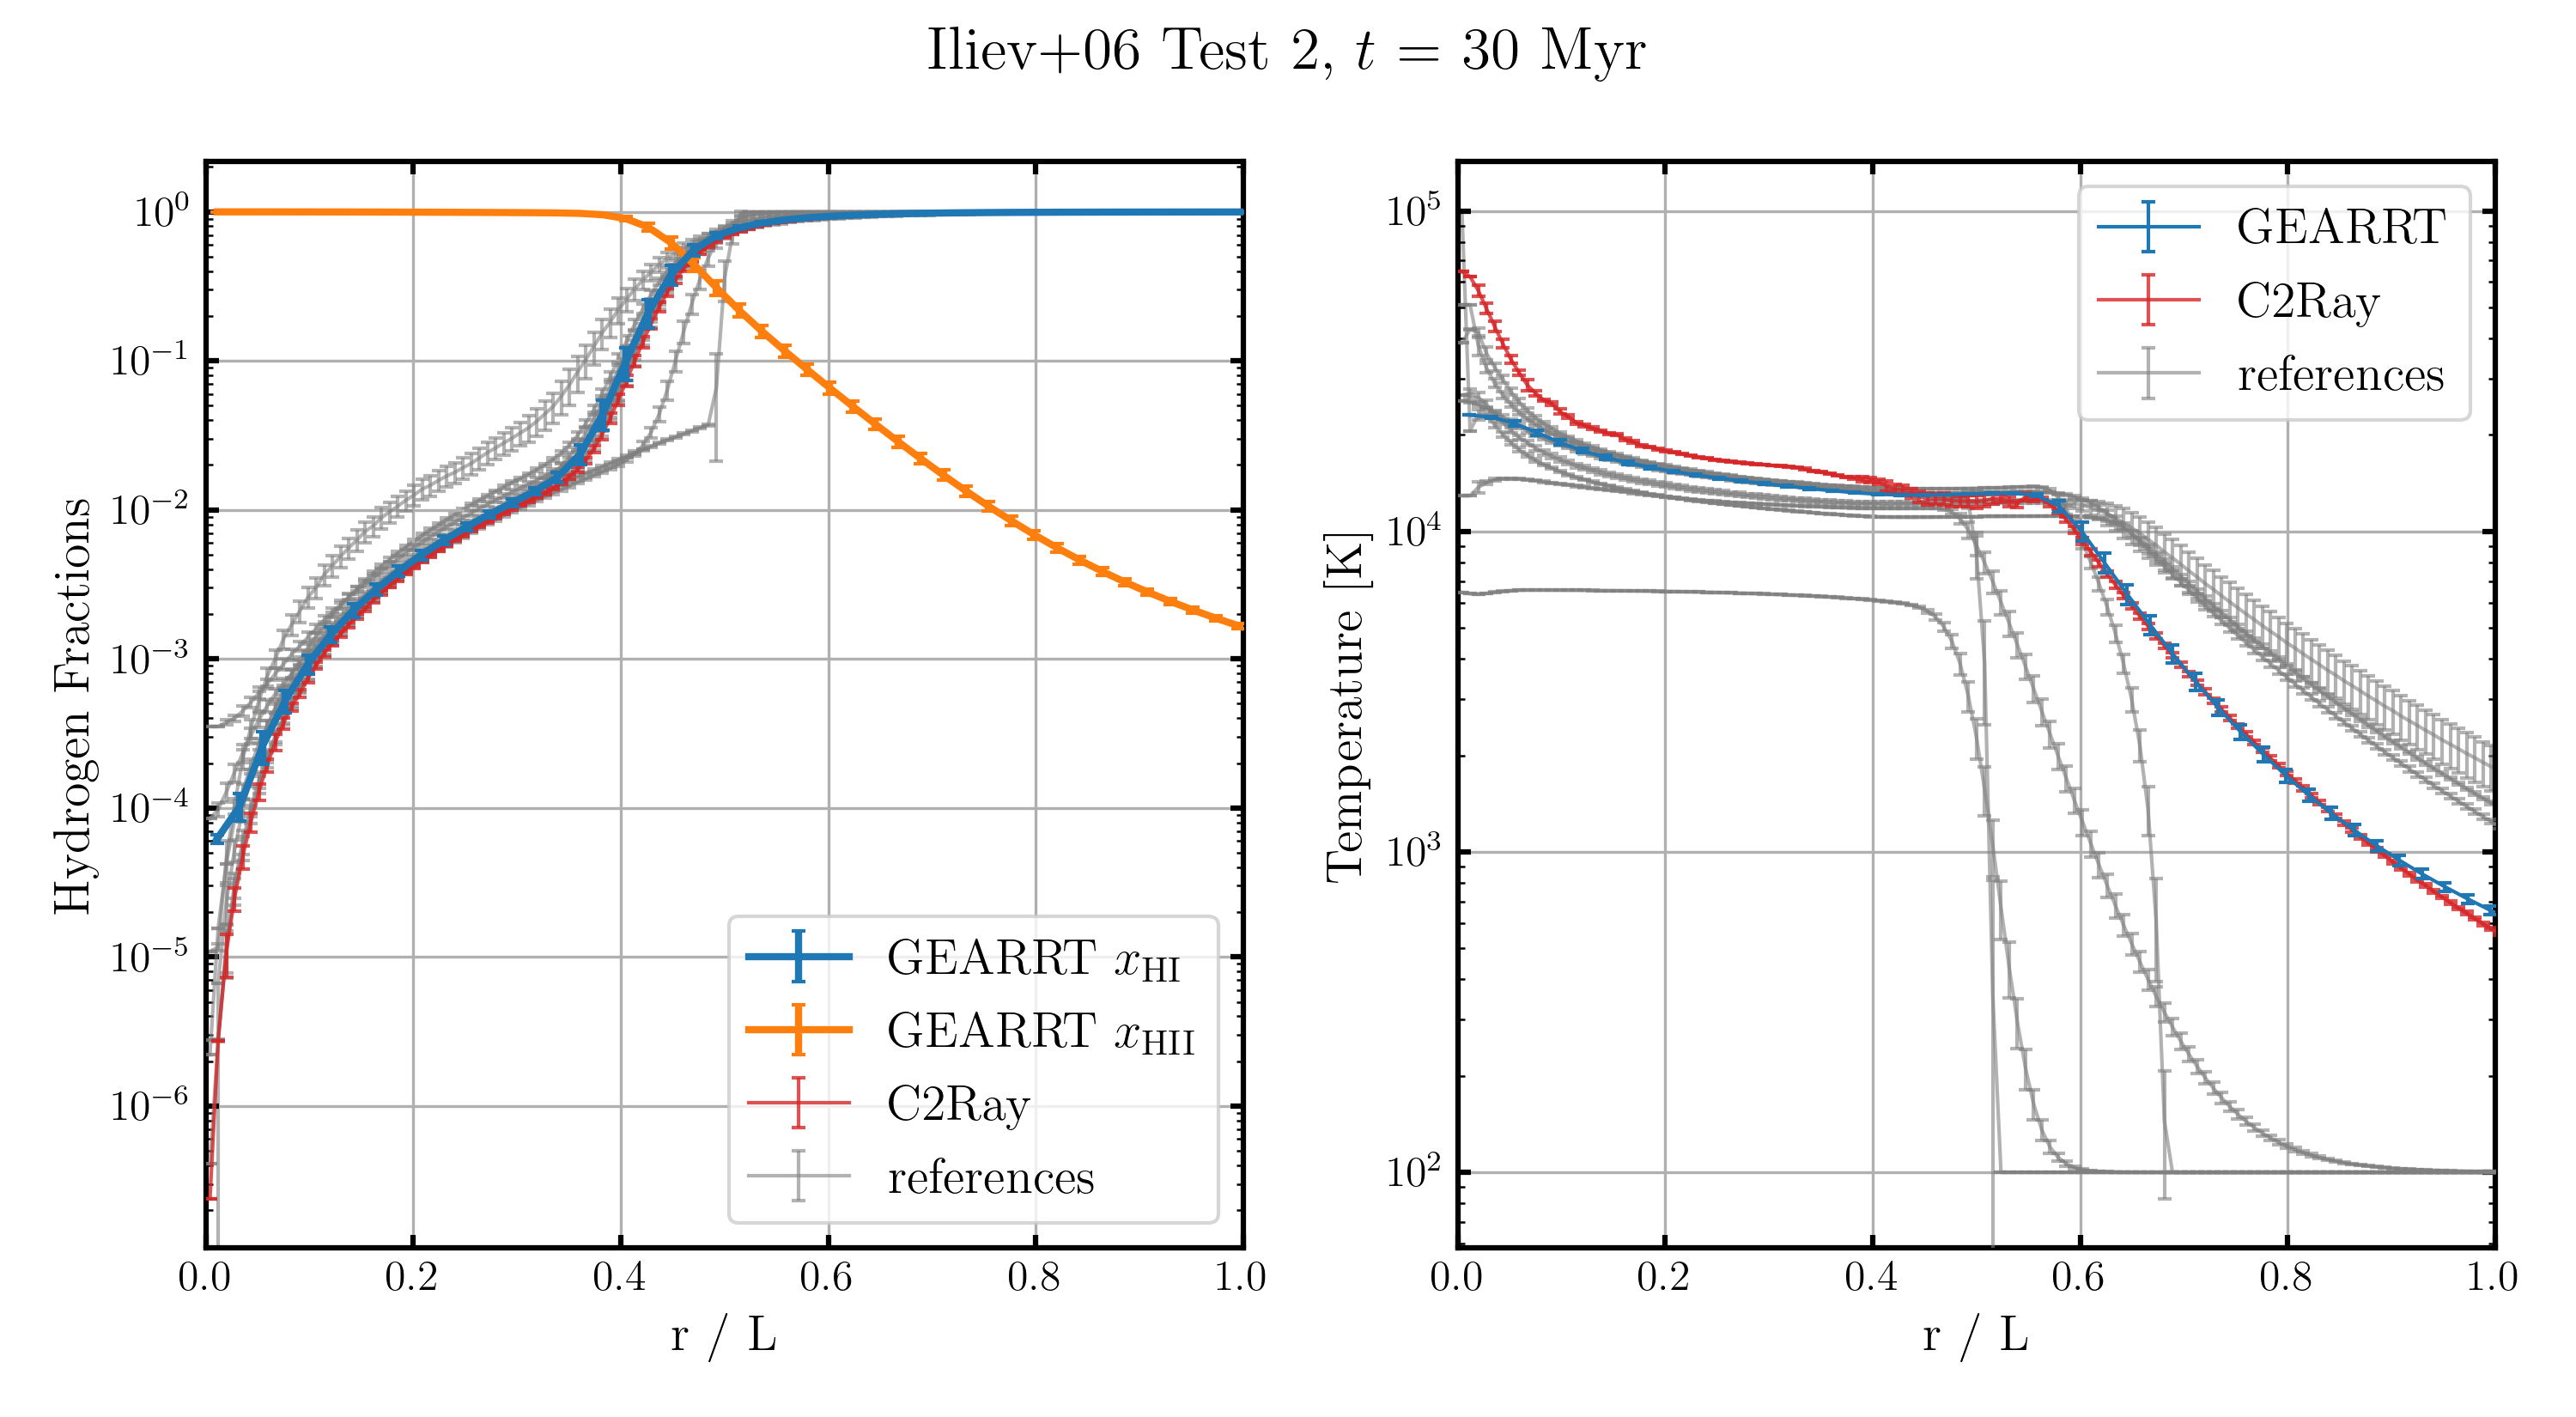
\includegraphics[width=.85\textwidth]{figures/RHD/Iliev2/output_0003.png}\\%
 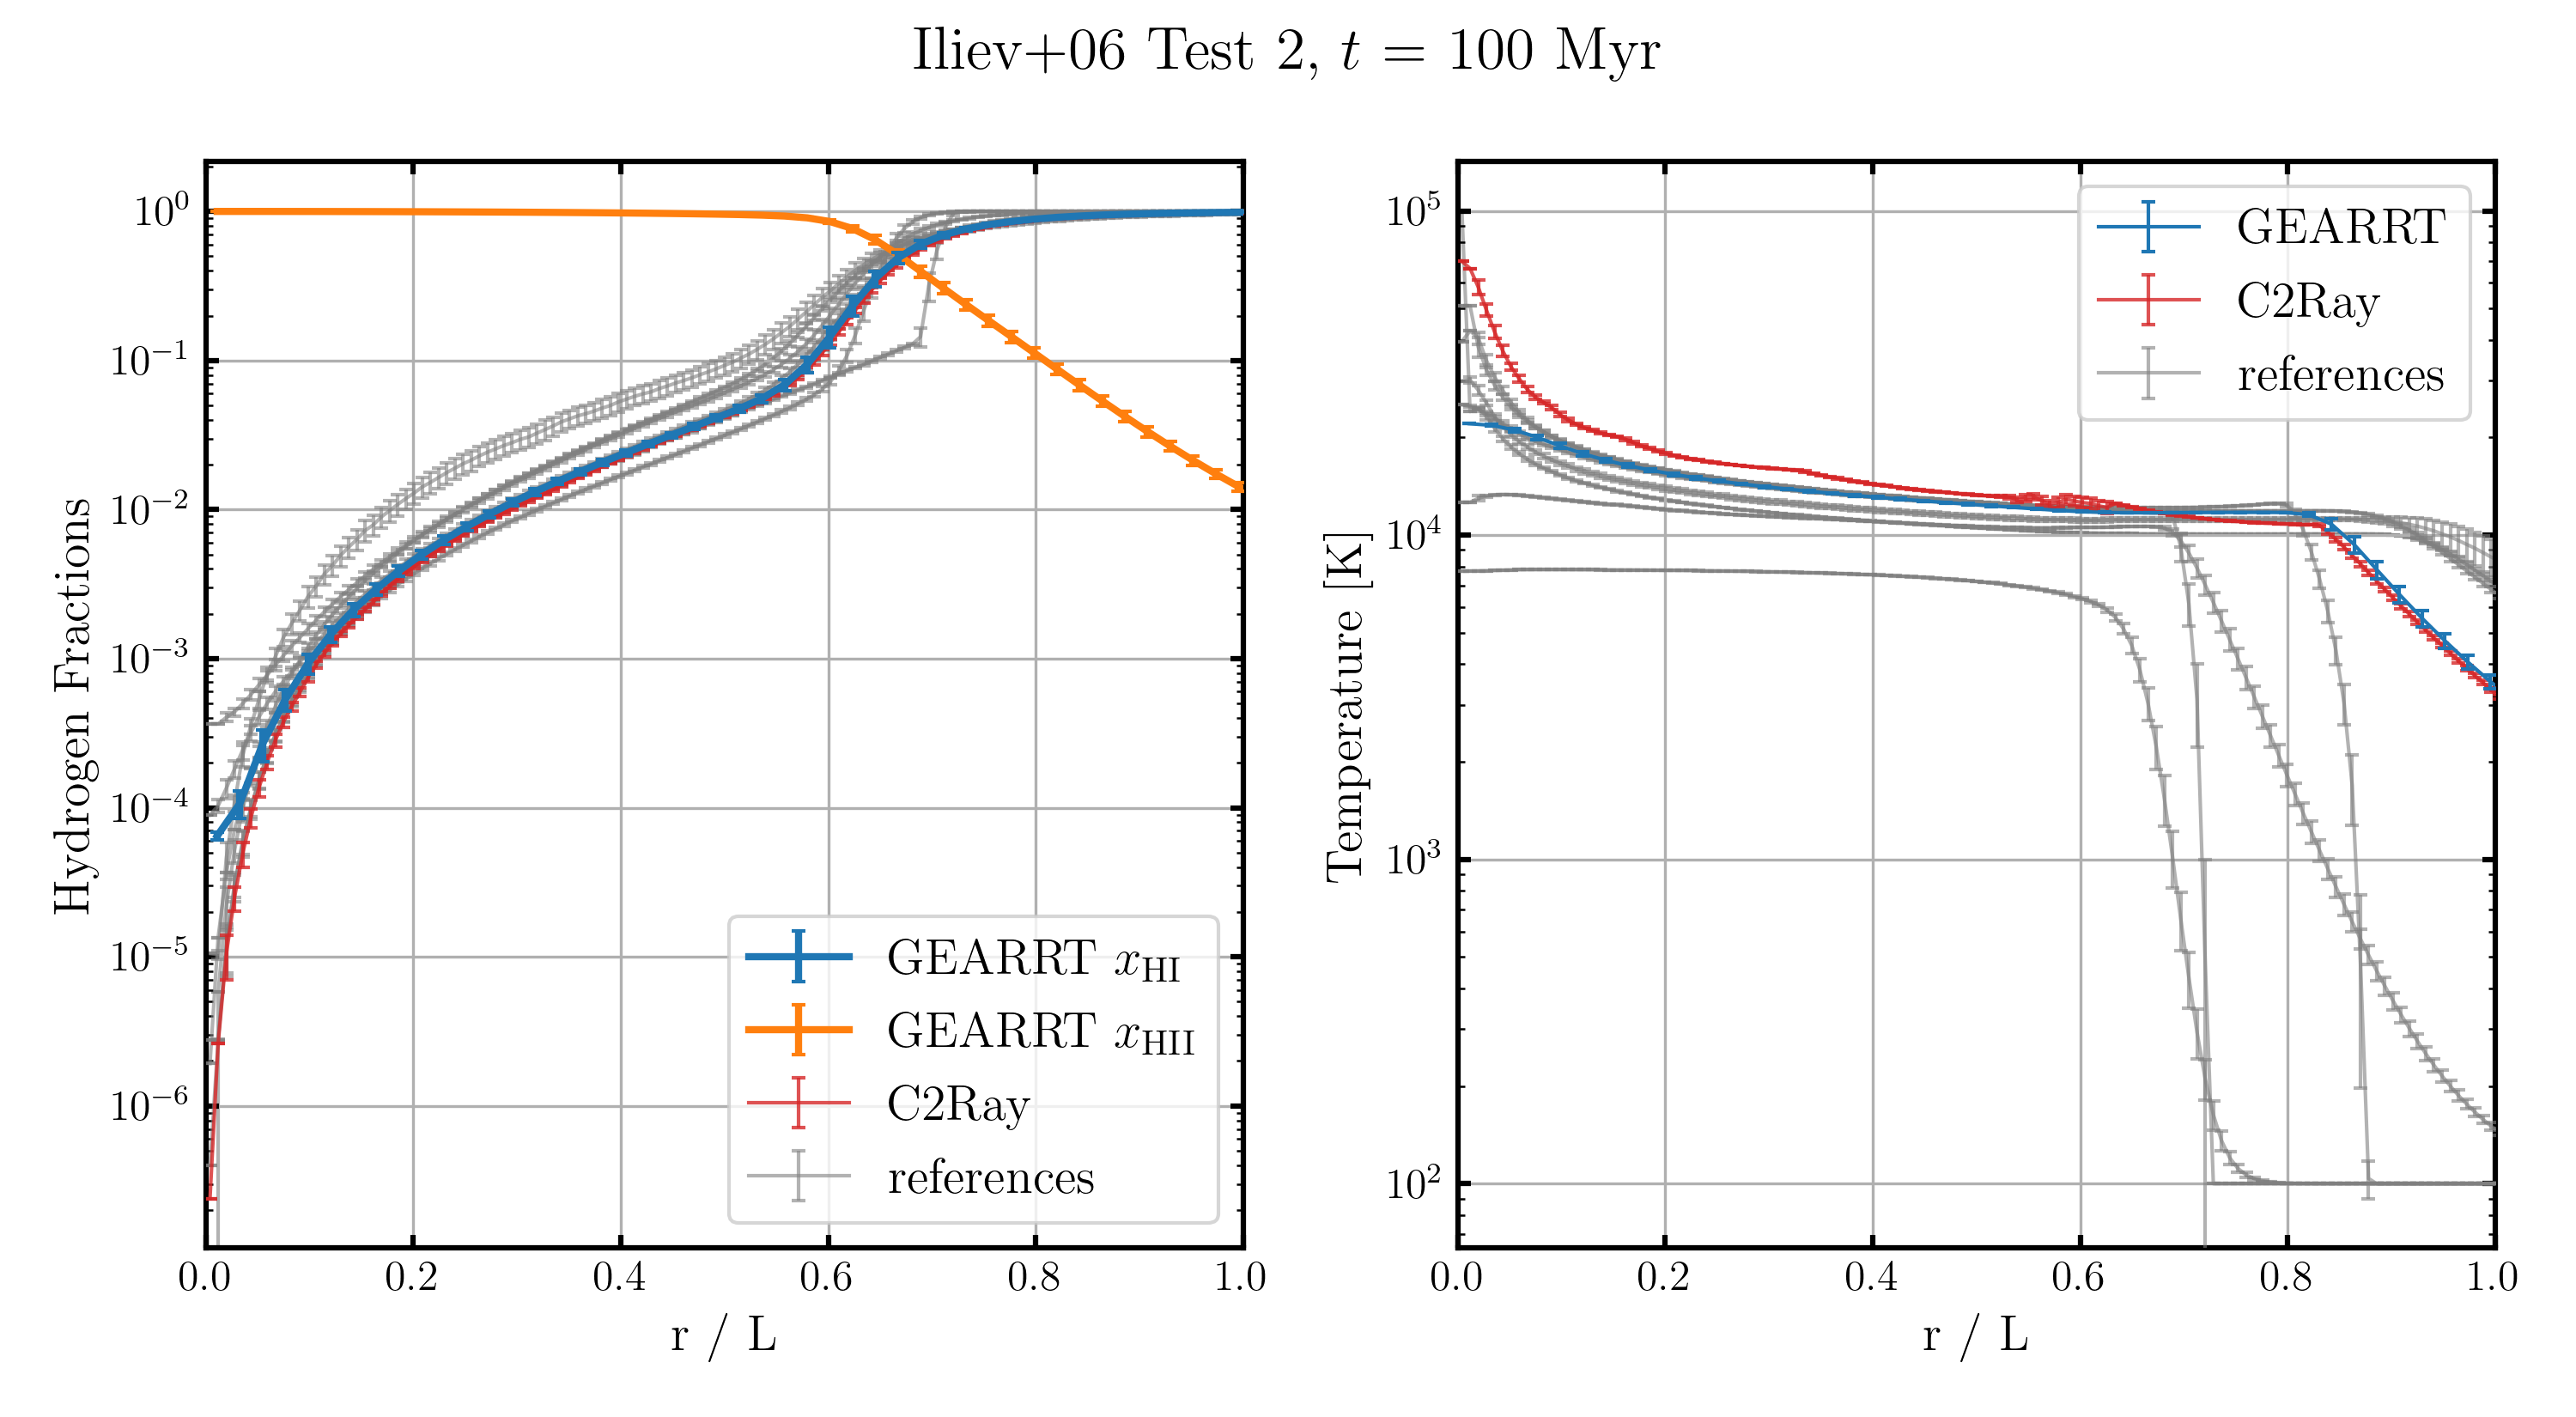
\includegraphics[width=.85\textwidth]{figures/RHD/Iliev2/output_0010.png}%
%  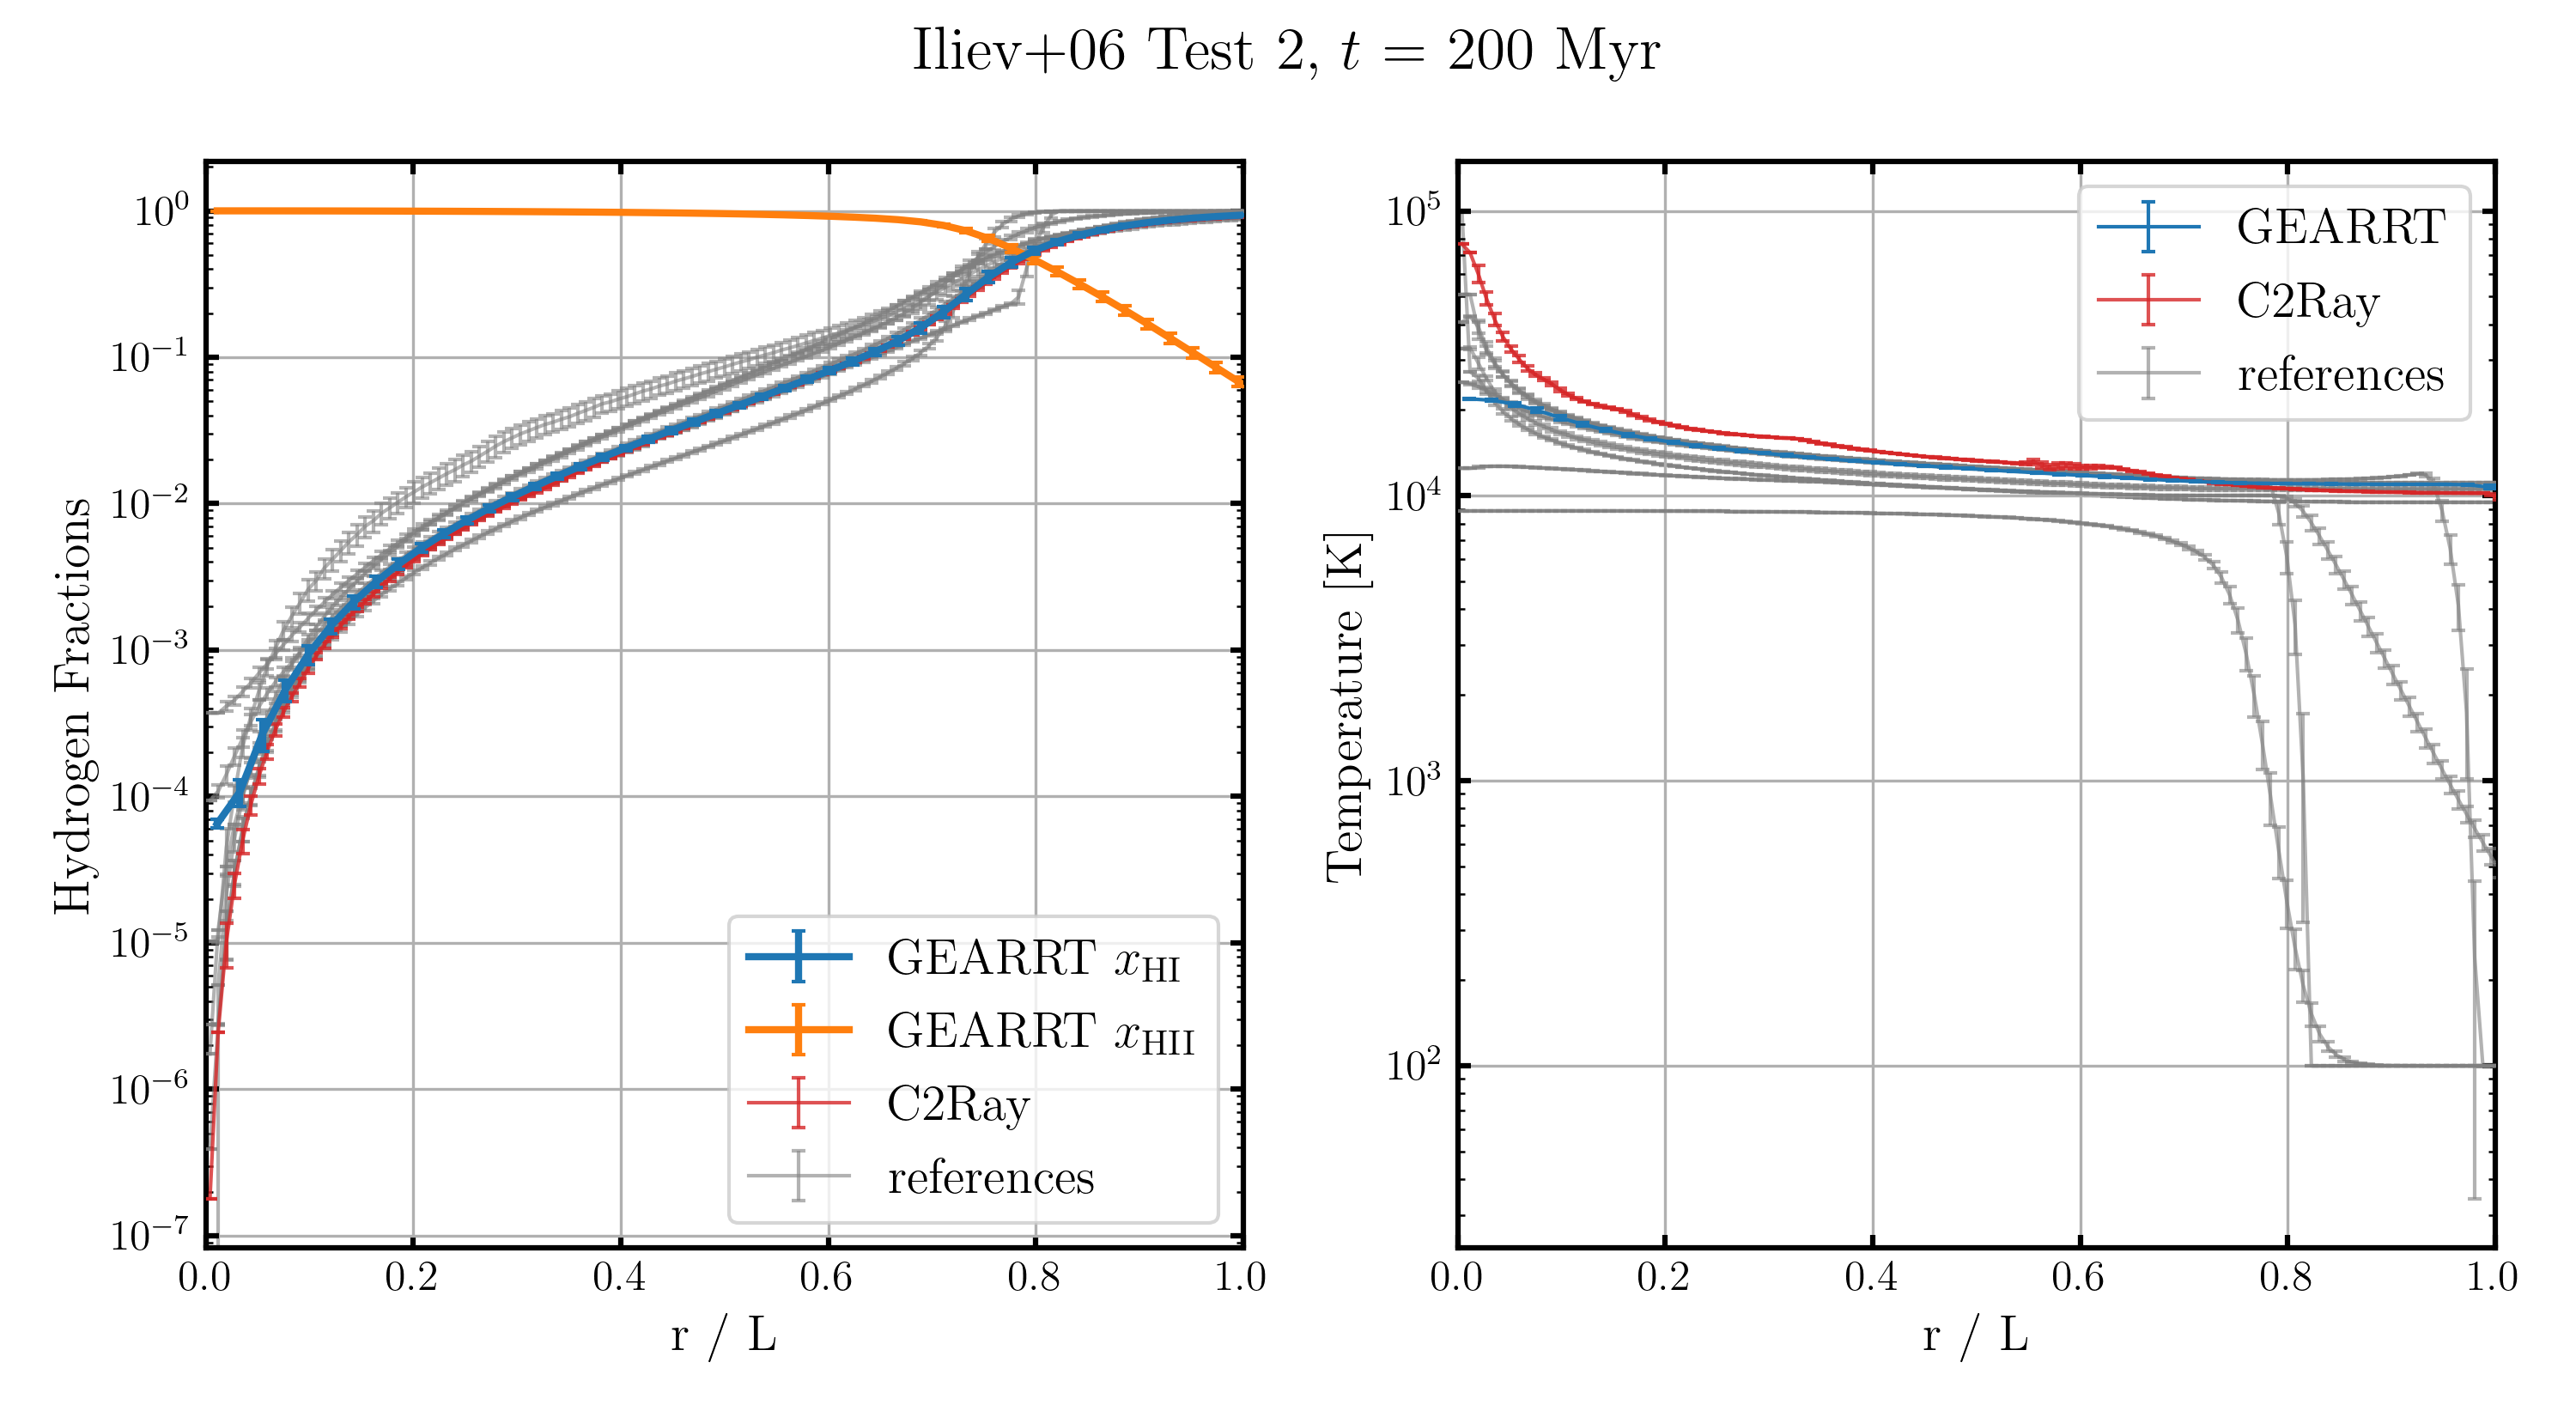
\includegraphics[width=\textwidth]{figures/RHD/Iliev2/output_0020.png}\\%
%  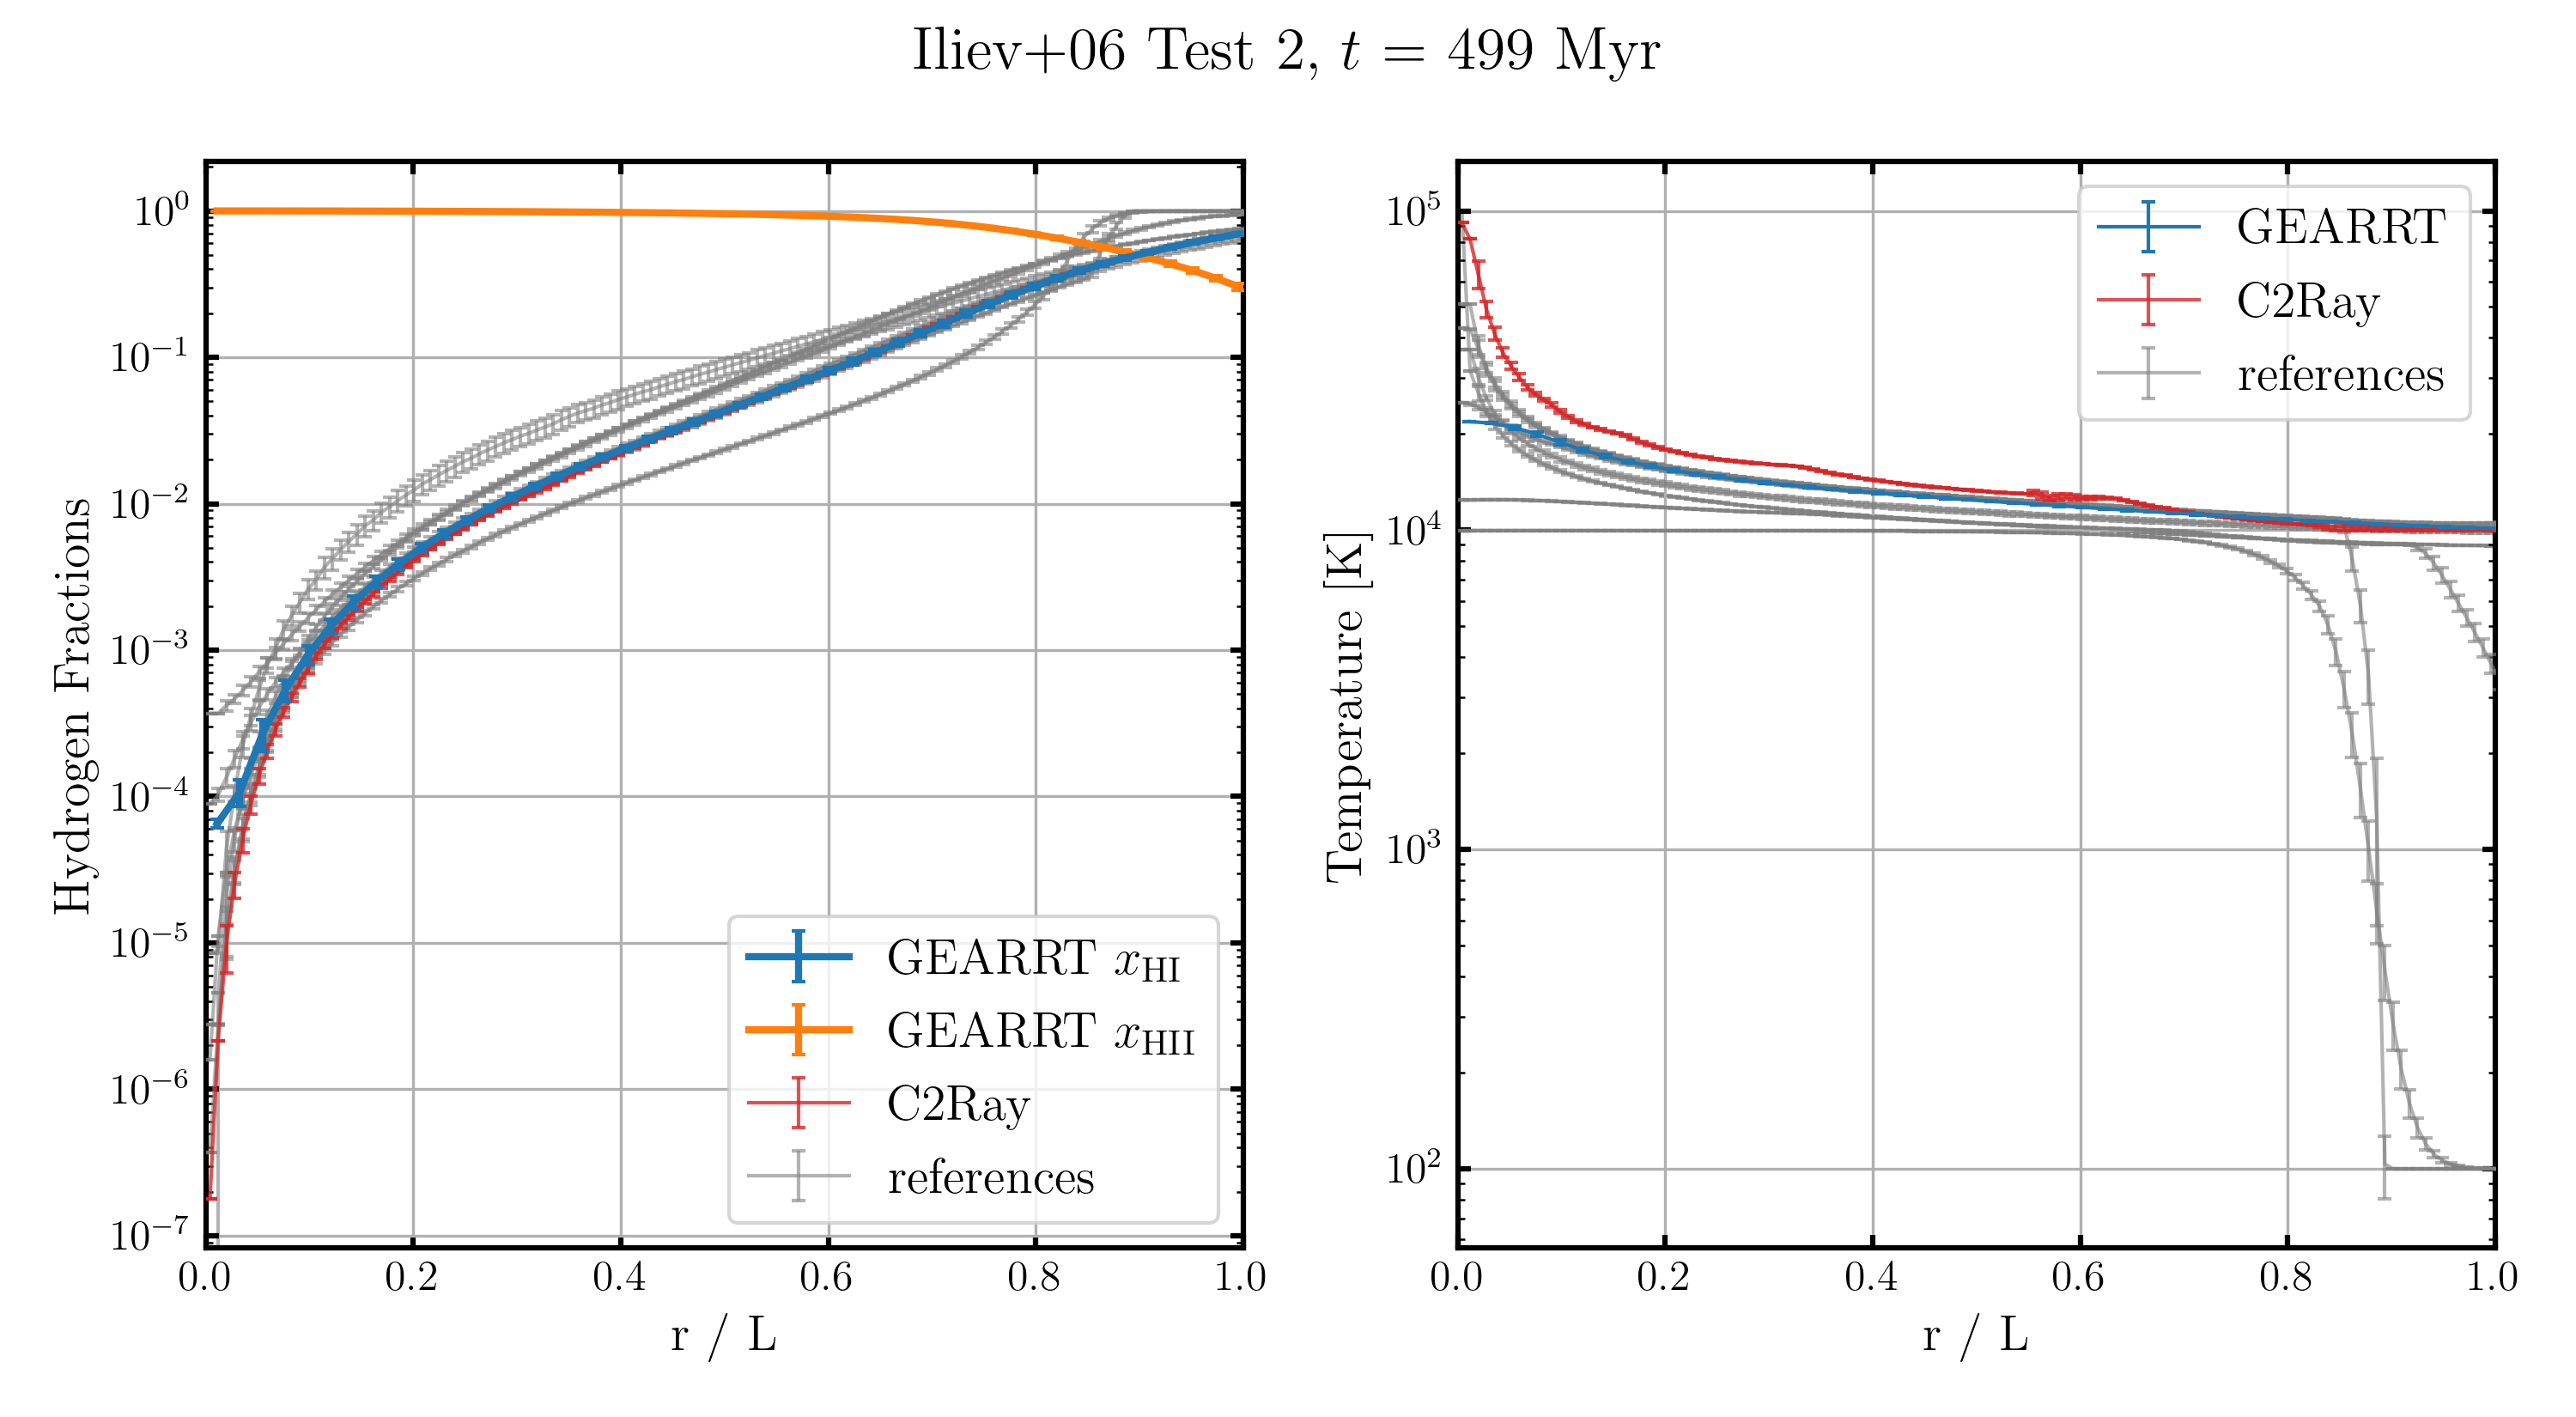
\includegraphics[width=\textwidth]{figures/RHD/Iliev2/output_0051.png}%
 \caption{
Spherically averaged Ionized and neutral fractions of hydrogen and temperatures in  Test 2 at 10,
30, and 100 Myr solved with \GEARRT and the reference solutions from IL6, where the solution of
\codename{C2Ray} has been highlighted. The error bars are standard deviations.
 }
 \label{fig:iliev2}
\end{figure}




\begin{figure}
 \centering
 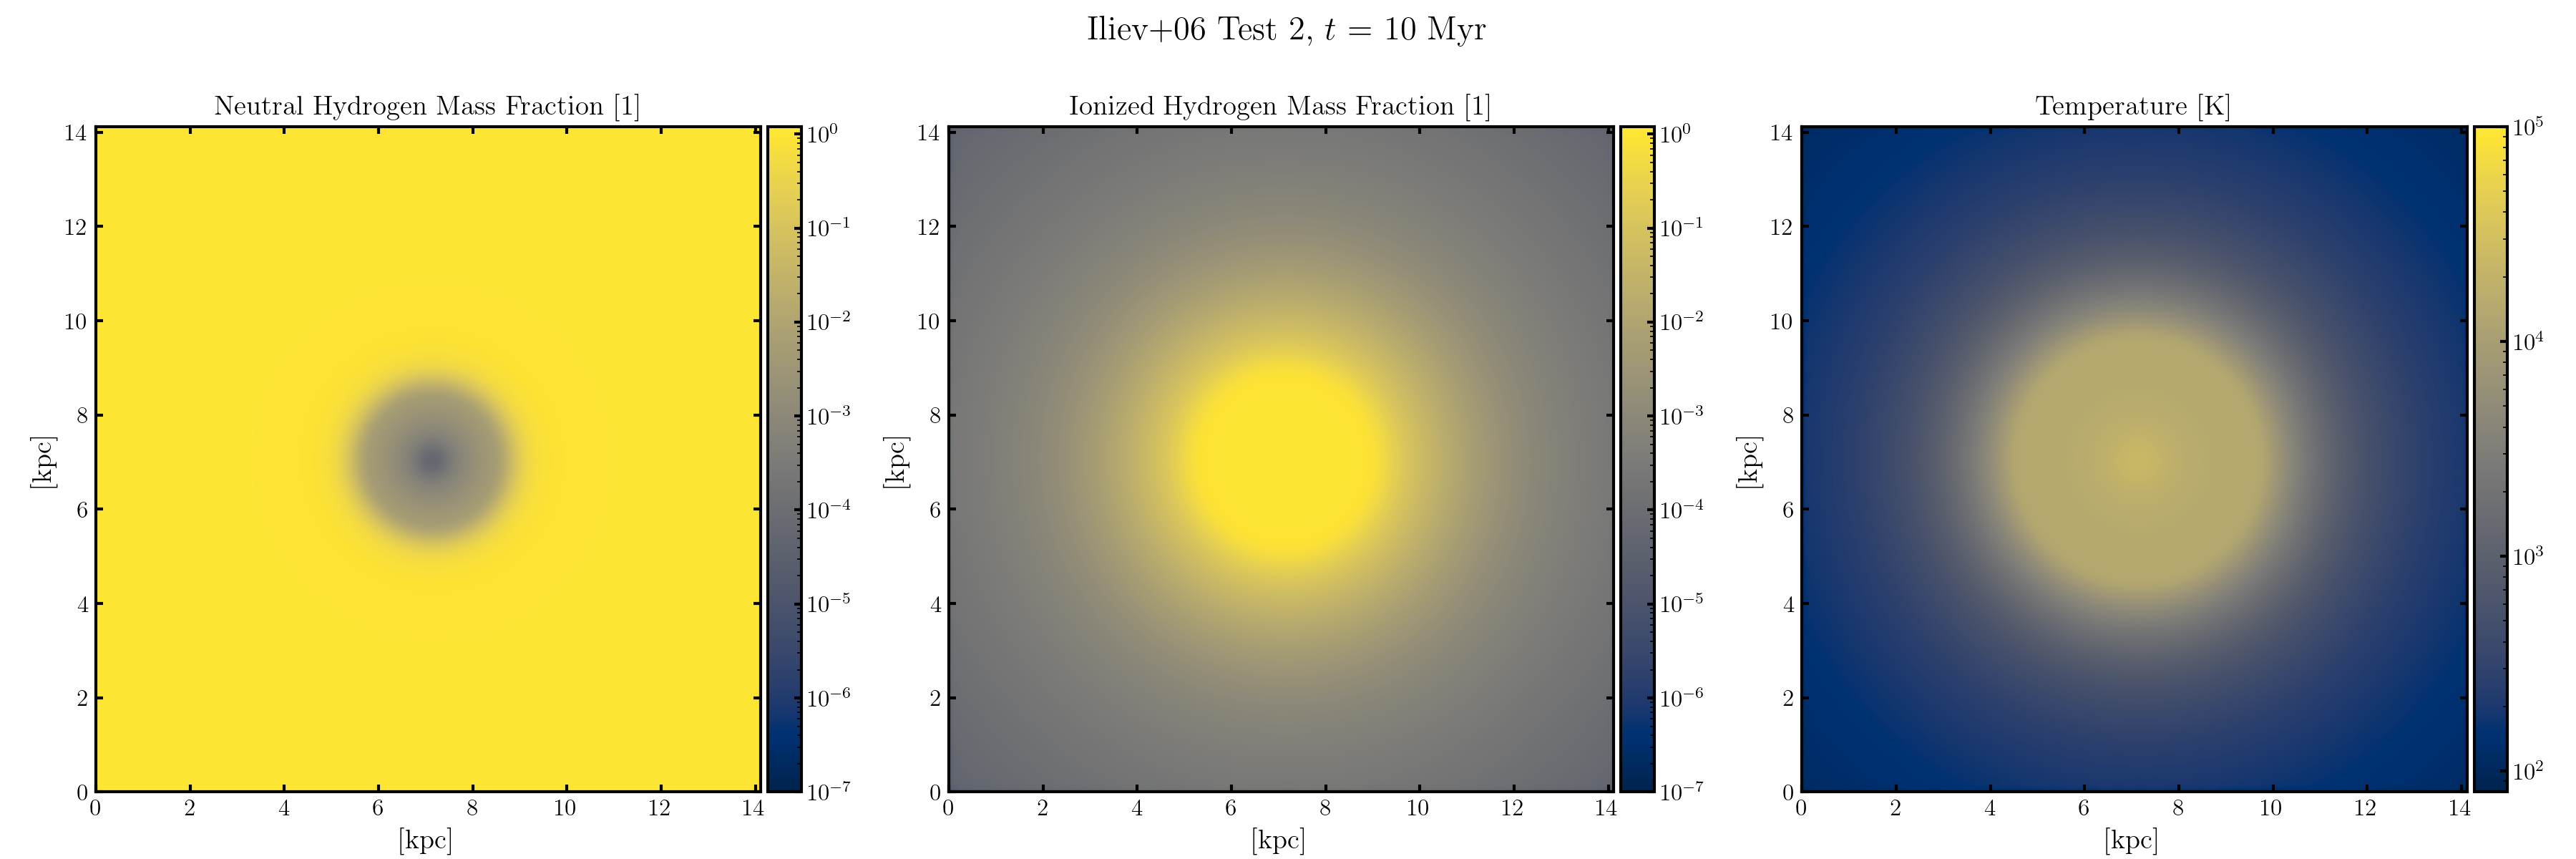
\includegraphics[width=\textwidth]{figures/RHD/Iliev2/output_0001-NoRef.png}\\%
 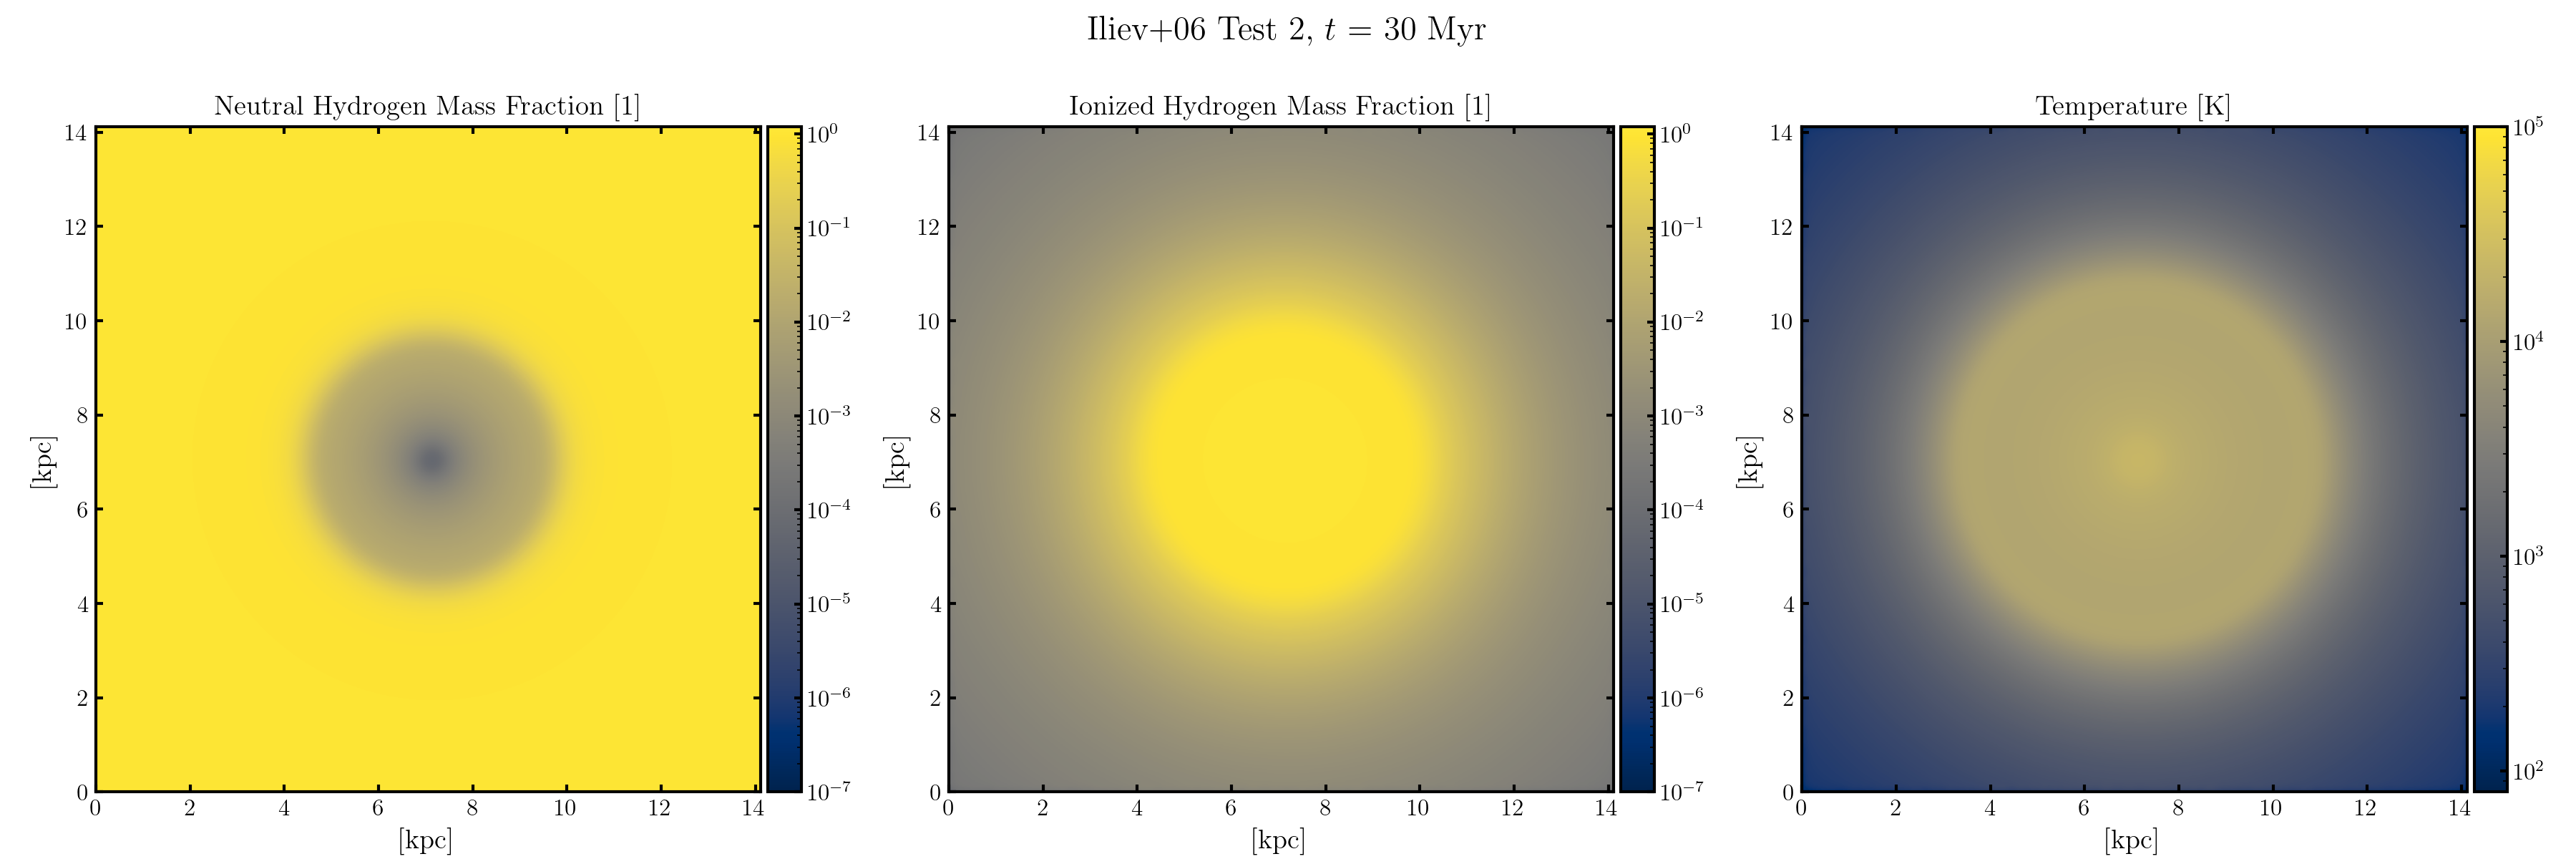
\includegraphics[width=\textwidth]{figures/RHD/Iliev2/output_0003-NoRef.png}\\%
 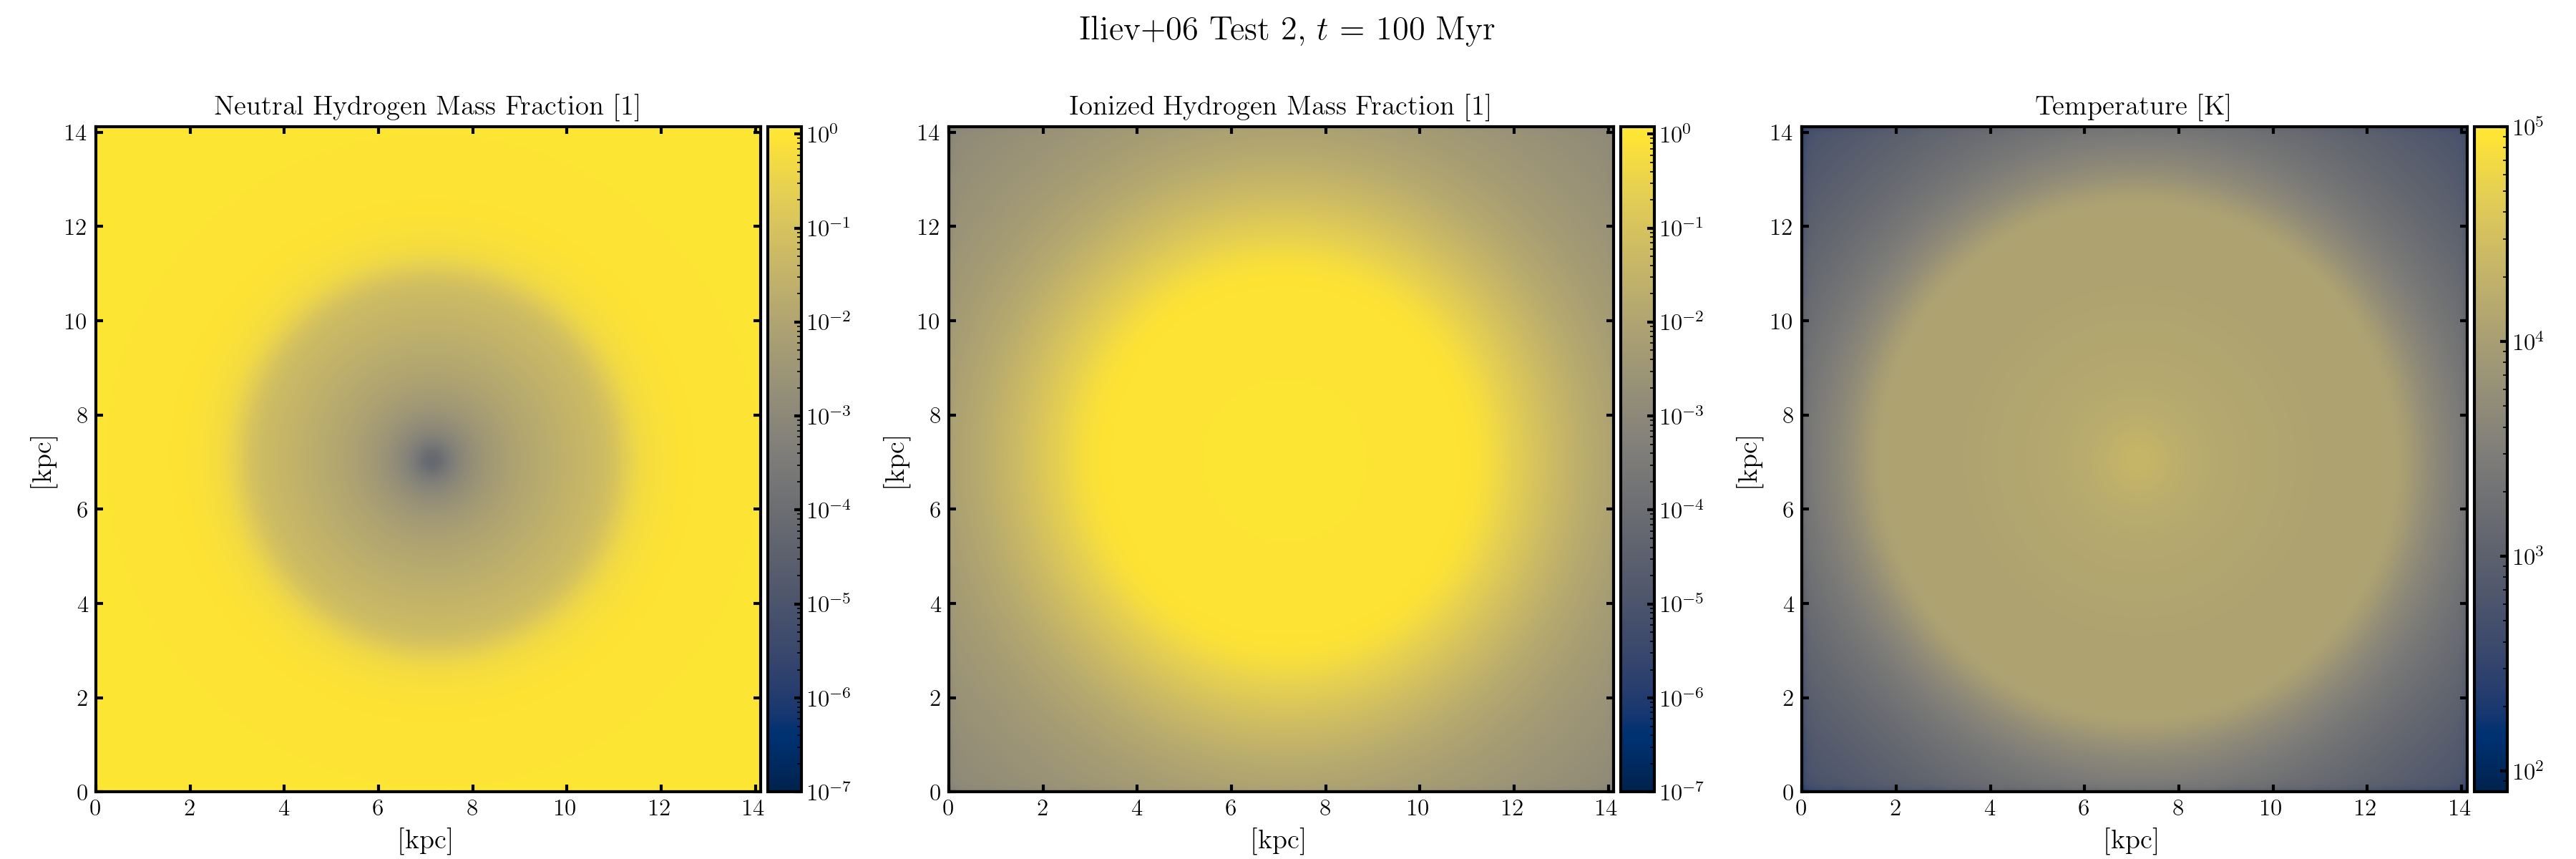
\includegraphics[width=\textwidth]{figures/RHD/Iliev2/output_0010-NoRef.png}\\%
 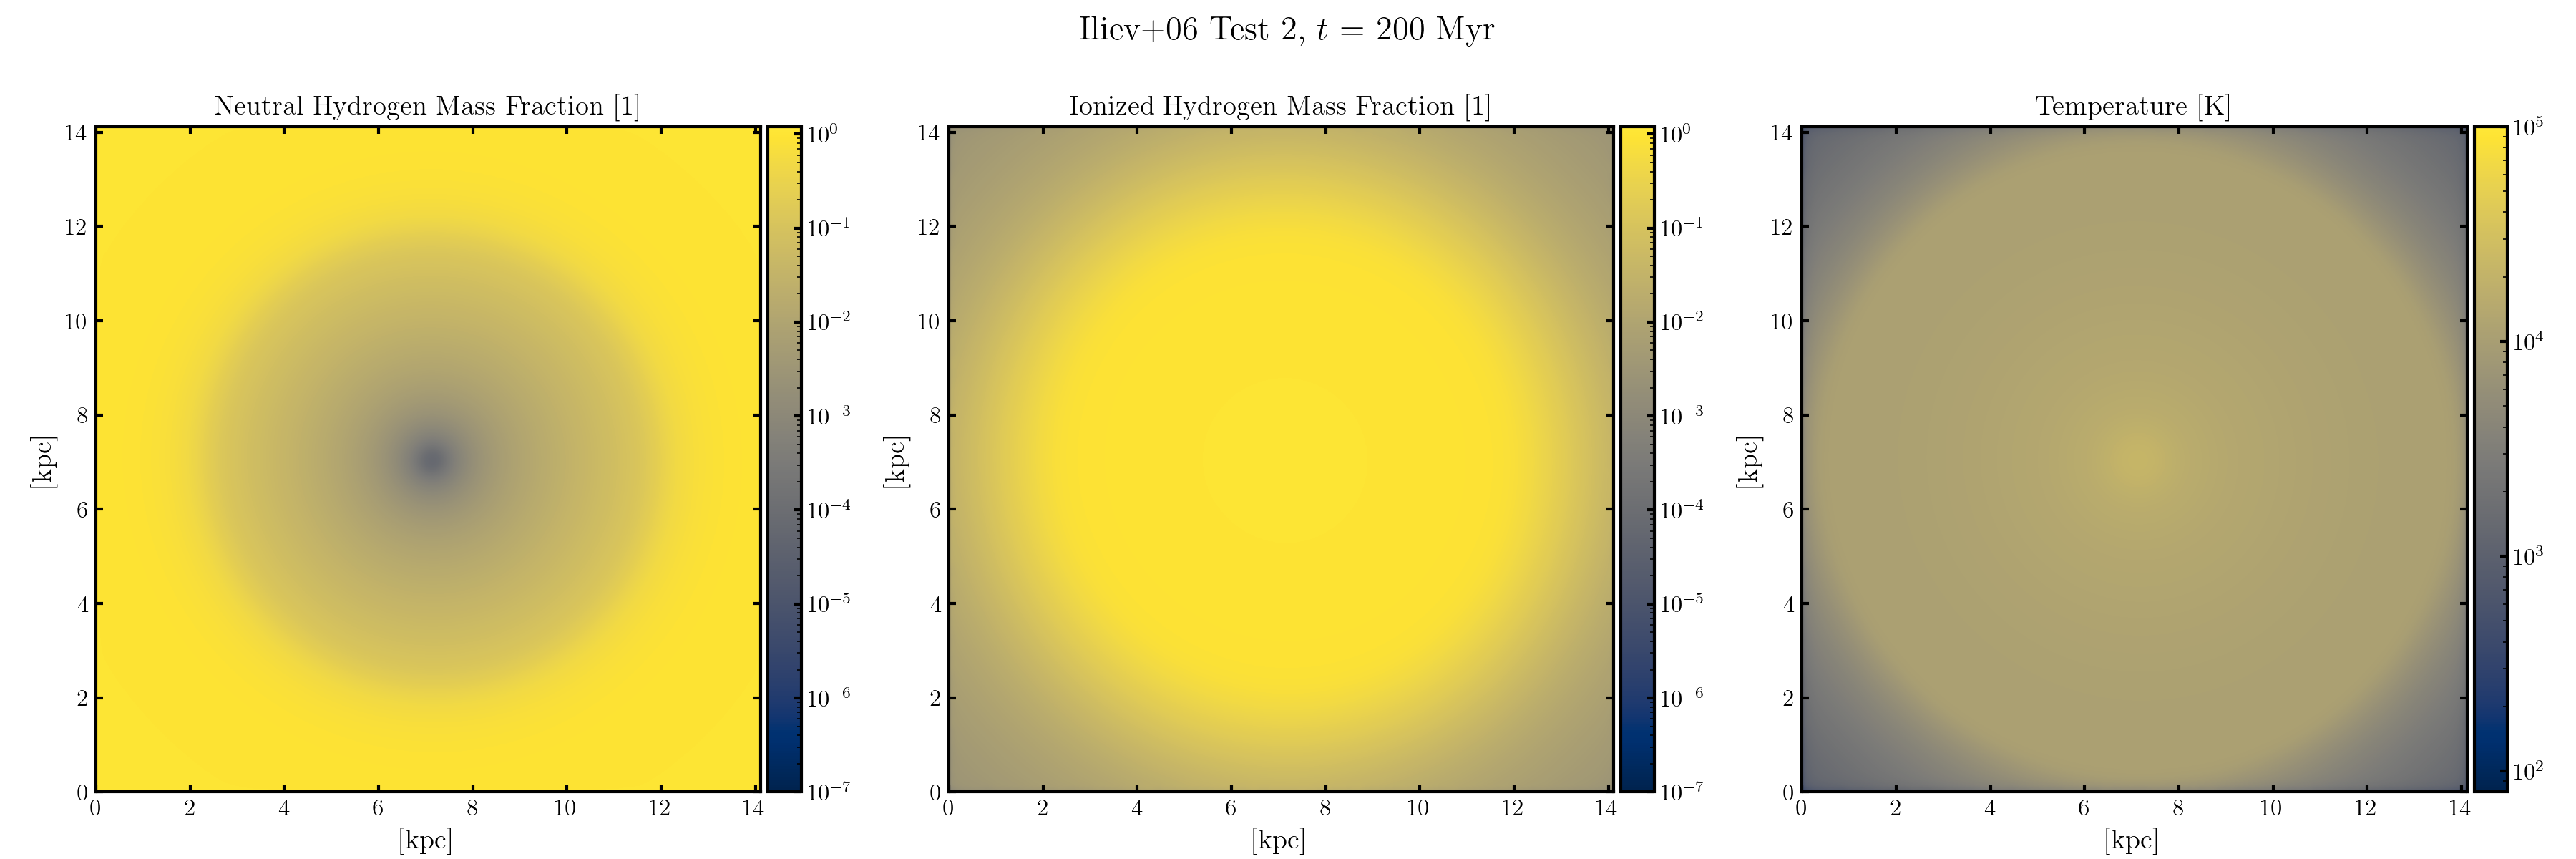
\includegraphics[width=\textwidth]{figures/RHD/Iliev2/output_0020-NoRef.png}%
%  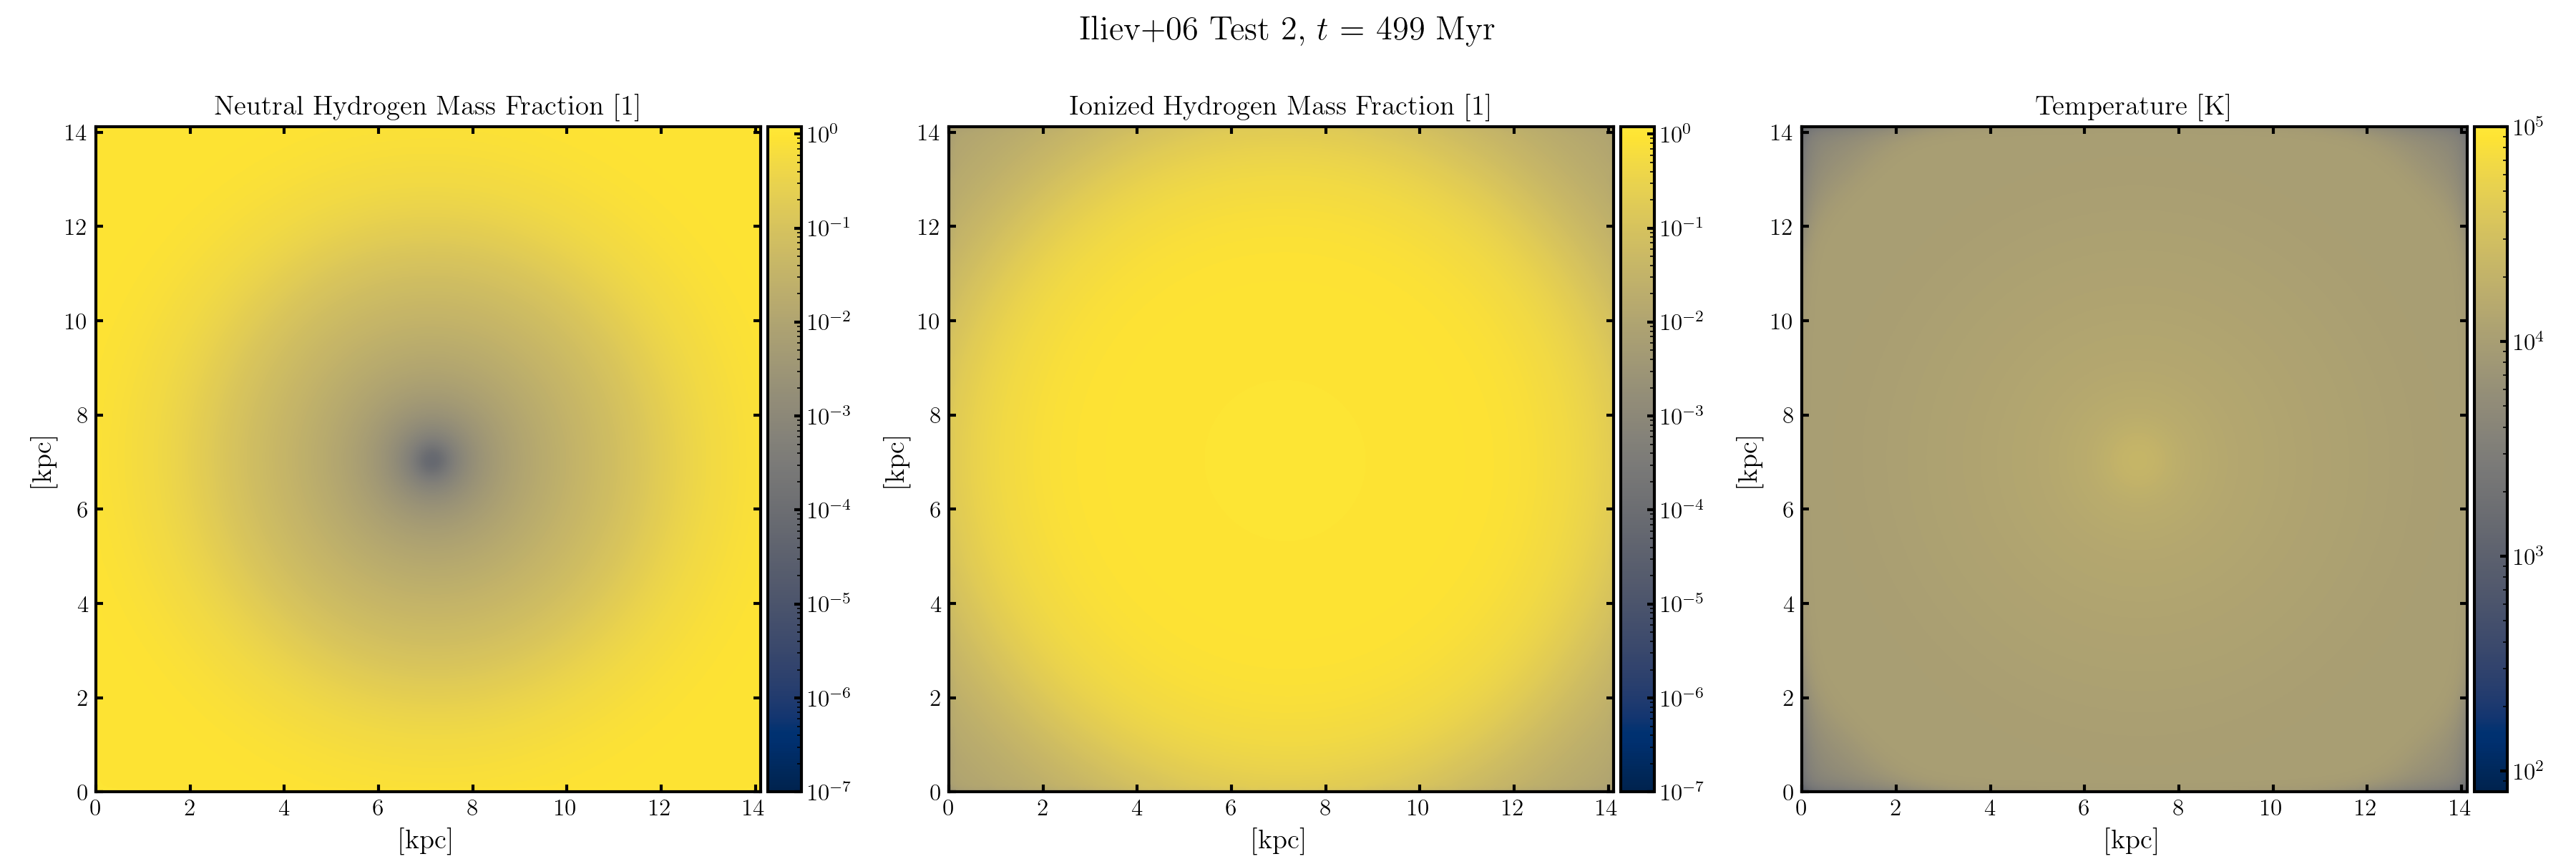
\includegraphics[width=\textwidth]{figures/RHD/Iliev2/output_0051-NoRef.png}%
 \caption{
Slices through the mid-plane of the box of the ionized and neutral fractions of hydrogen and
temperatures in Test 2 at 10, 30, 100, and 200 Myr solved with \GEARRT.
 }
 \label{fig:iliev2-slices}
\end{figure}





\begin{figure}
 \centering
 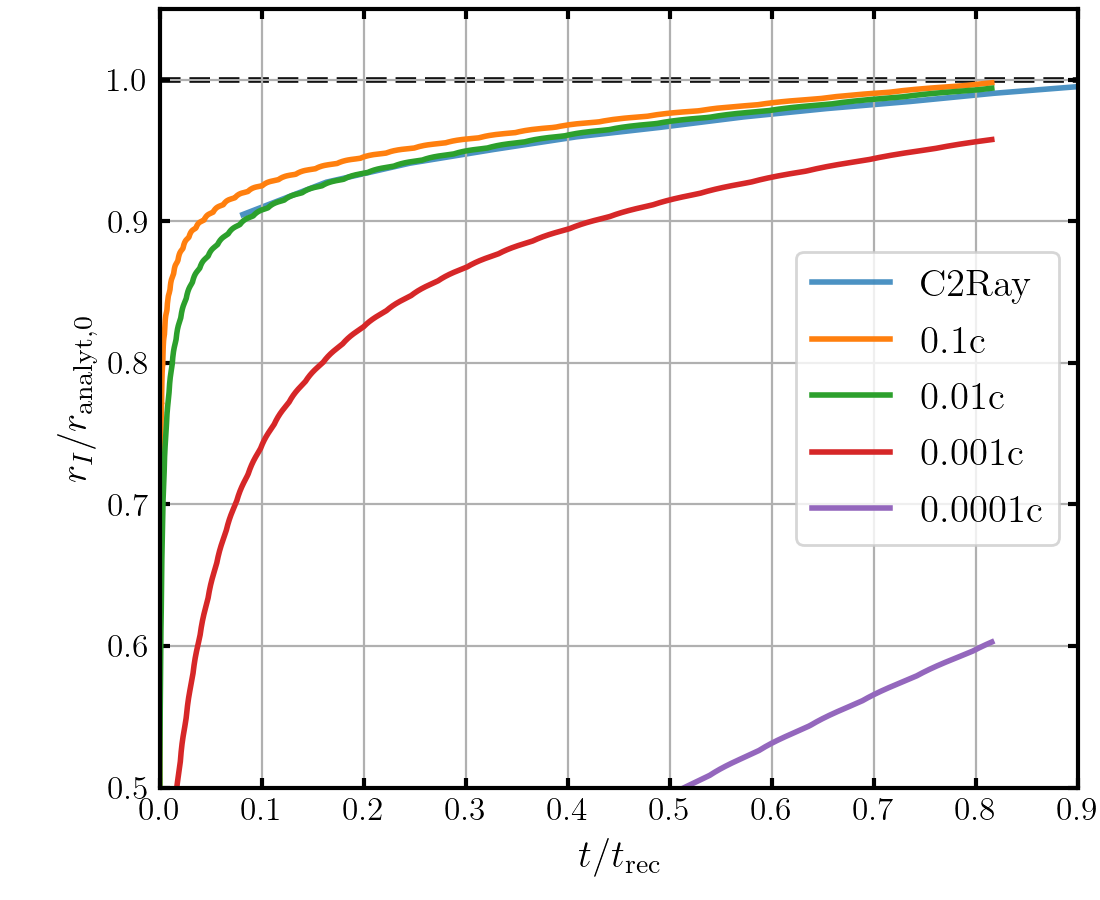
\includegraphics[width=.7\textwidth]{figures/RHD/Iliev2/ionization_fronts_compare_C.png}%
 \caption{
 The position of the ionization front for the Test 2 over 100 Myr with different values for the
reduced speed of light, as indicated in the legend, compared to the expected analytical position
given in eq.~\ref{eq:rI}, along with the solution of \codename{C2Ray}, which assumed an infinite
speed of light.
 }
 \label{fig:iliev2-compare-c}
\end{figure}



\begin{figure}
 \centering
 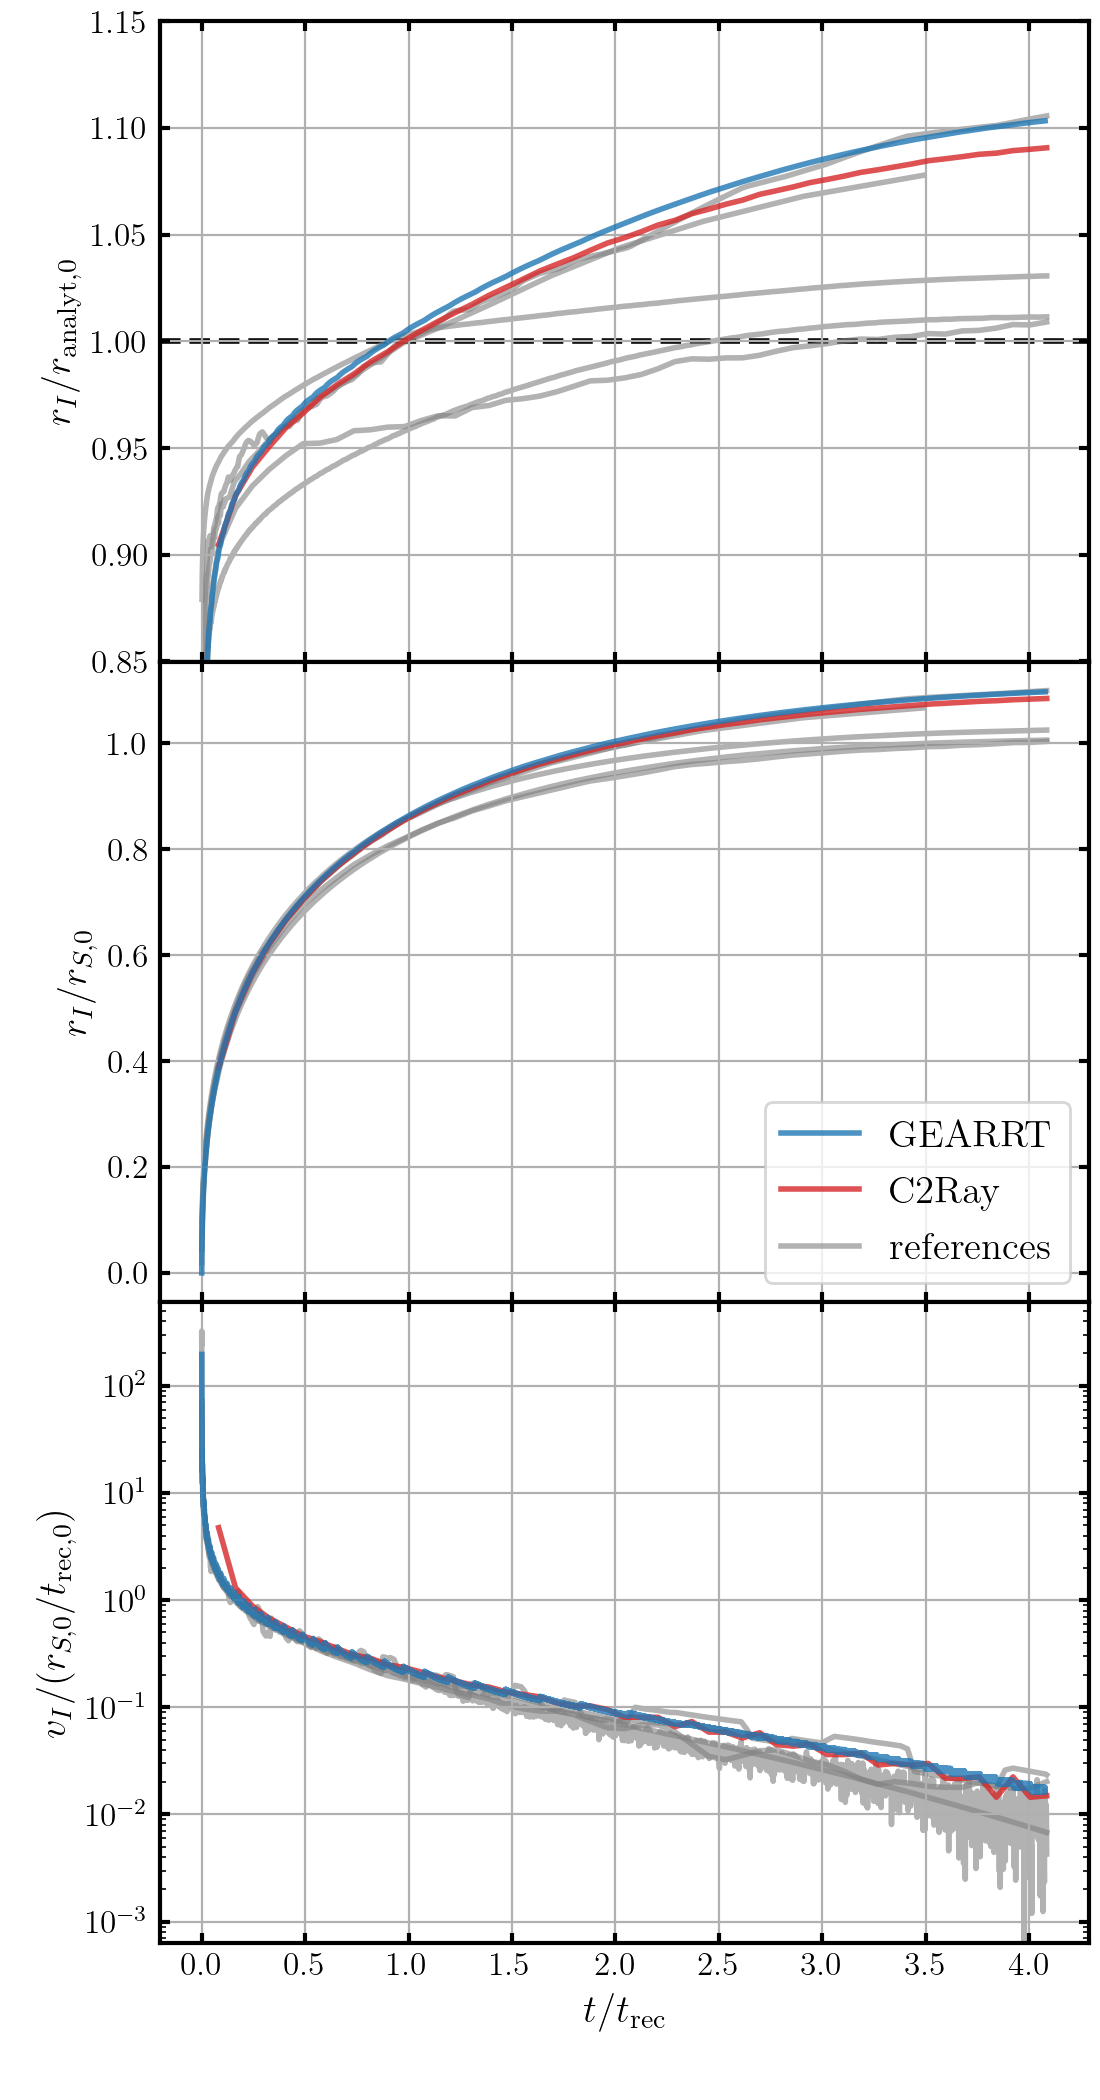
\includegraphics[width=.7\textwidth]{figures/RHD/Iliev2/ionization_fronts.png}%
 \caption{
 Evolution of the I-front position and velocity over time for Test 2.
 Top: Evolution of the I-front position over time, compared to the analytical position of Test 1
(eq.~\ref{eq:rI}).
 Middle: Evolution of the I-front position over time, compared to the final Str\"omgren radius
(eq.~\ref{eq:rS}).
 Bottom: Evolution of the I-front velocity.
 }
 \label{fig:iliev2-Ifront}
\end{figure}


\begin{figure}
 \centering
 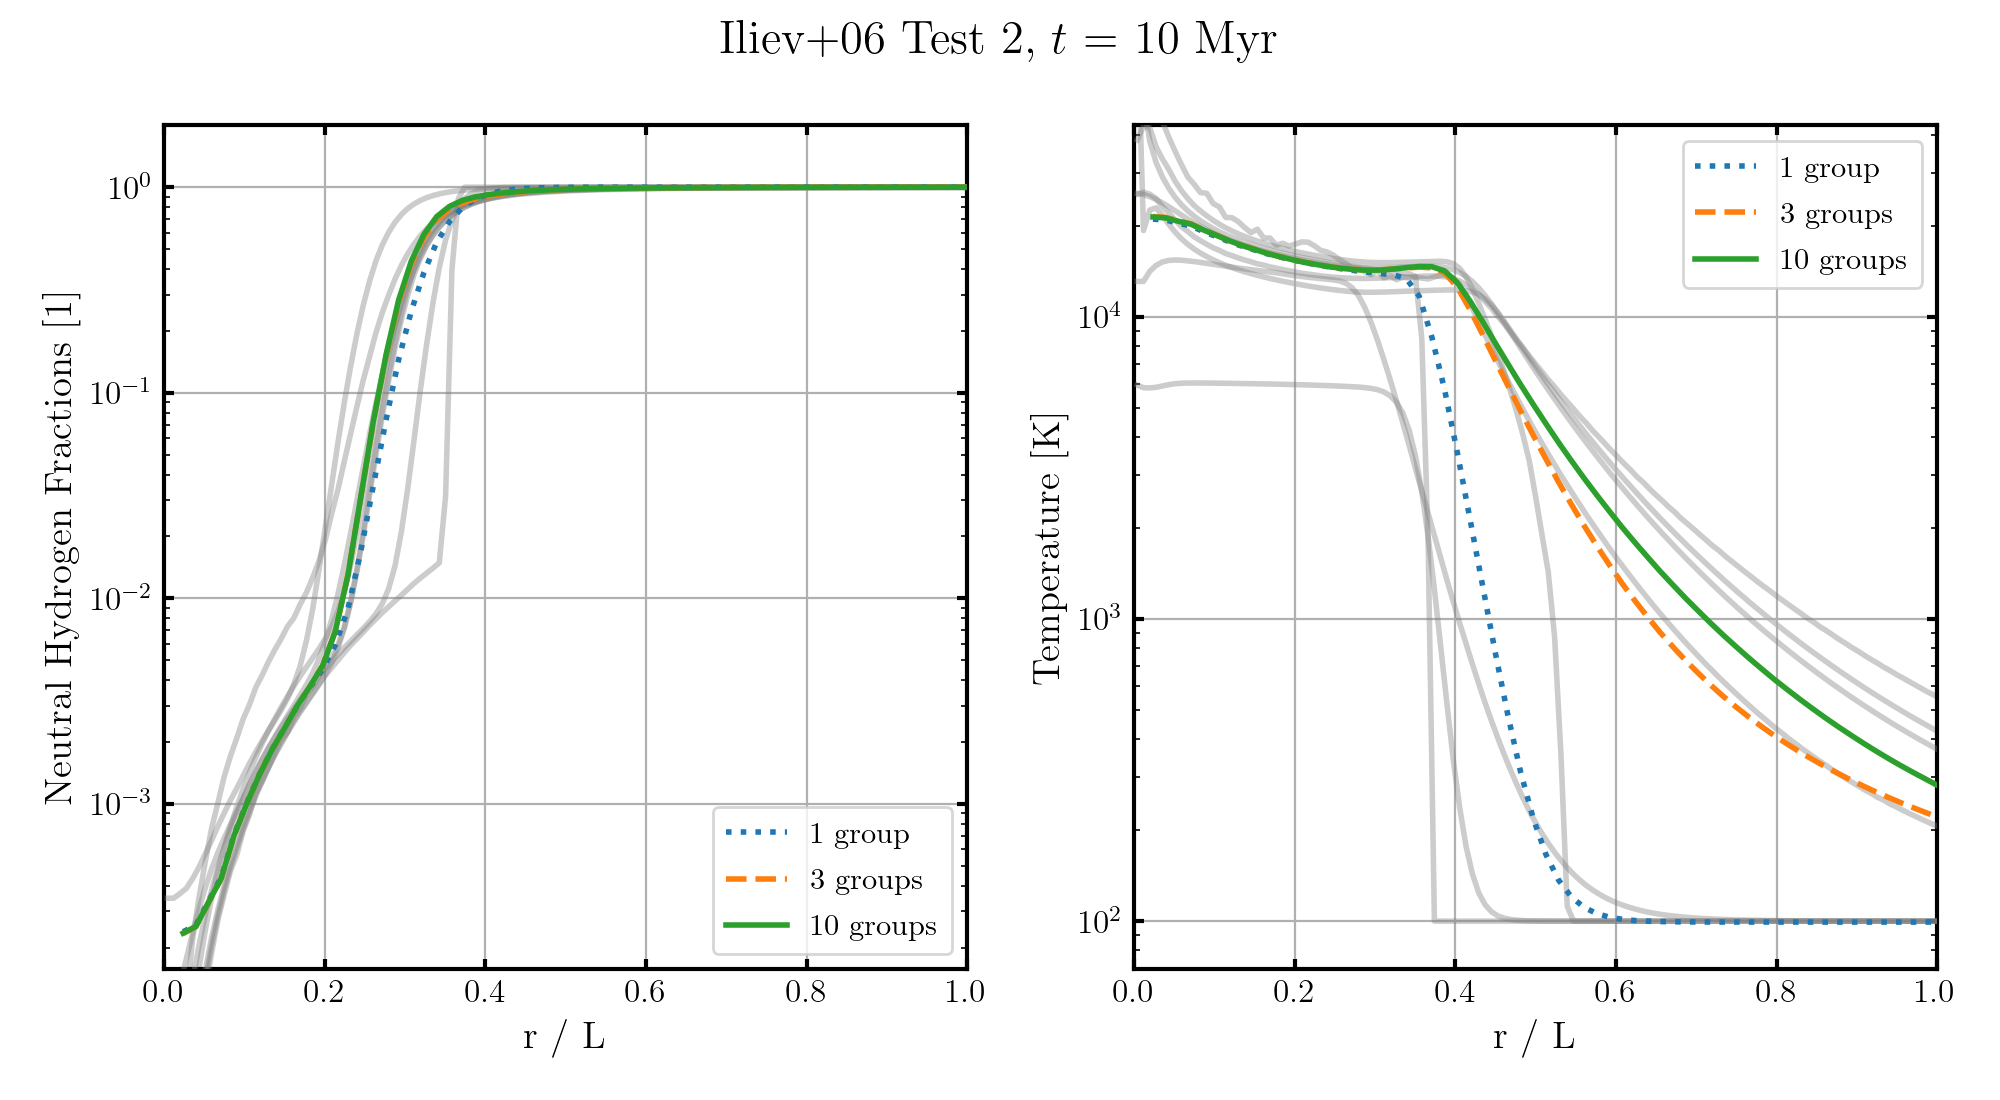
\includegraphics[width=\textwidth]{figures/RHD/Iliev2/photon_groups.png}%
 \caption{
Spherically averaged ionized and neutral fractions of hydrogen and temperatures of Test 2 at 10
Myr for 1, 3, and 10 photon frequency groups used. With an increasing number of groups, the
approximation becomes more accurate and closer to treating frequencies individually. The average
ionization cross sections are treated more accurately, and high energy photons have lower
interaction rates, as they should. The high energy photons are then able to reach regions further
from the source, where they can heat the gas.
 }
 \label{fig:iliev2-photon-groups}
\end{figure}




\begin{figure}
 \centering
 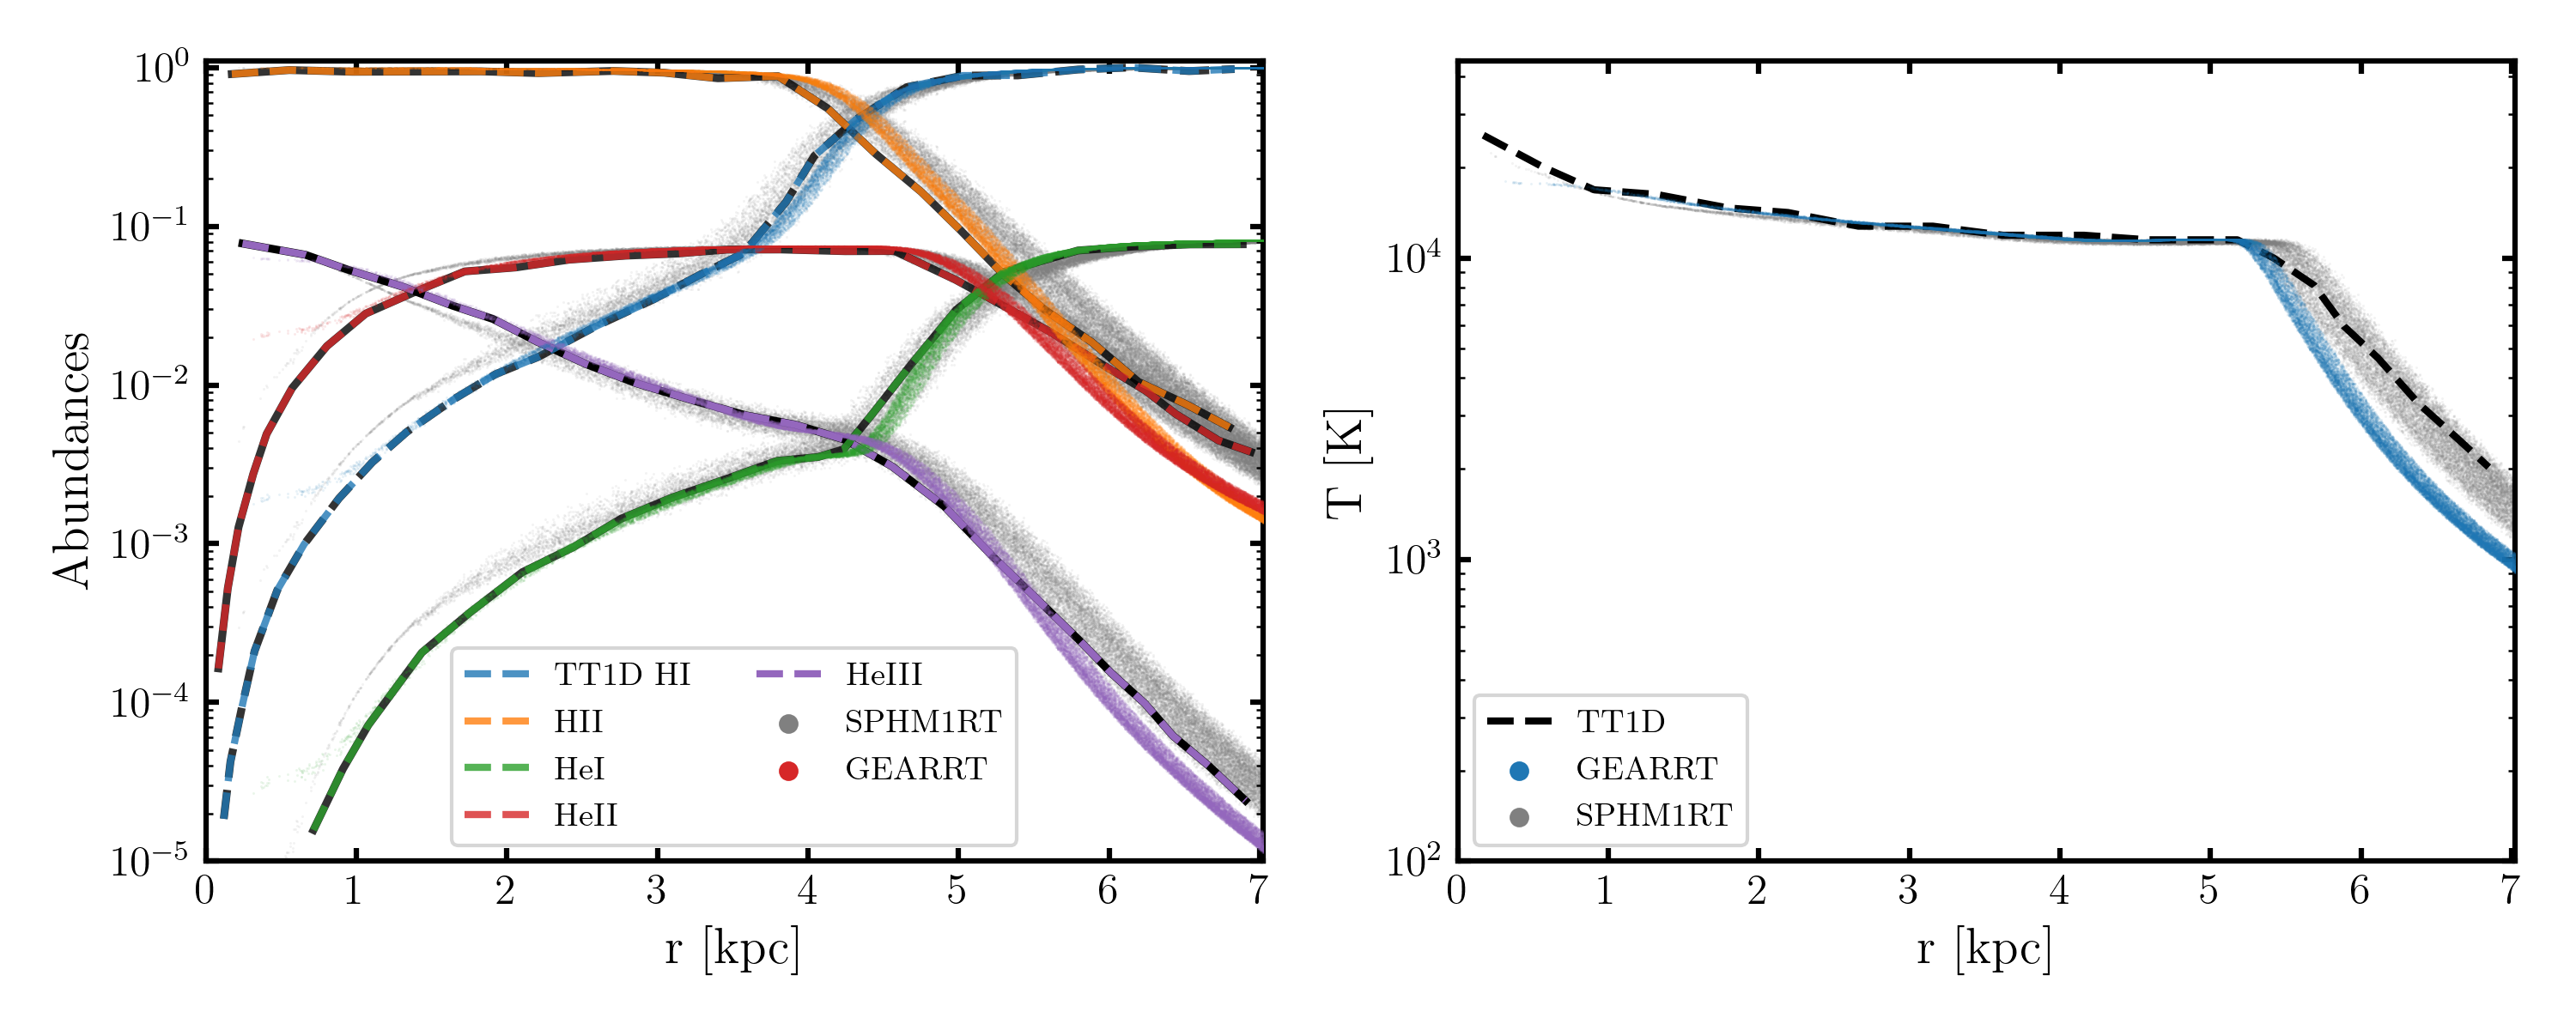
\includegraphics[width=\textwidth]{figures/RHD/Iliev2/HHe.png}%
 \caption{
Spherically averaged ionized and neutral fractions of hydrogen and helium of Test 2 at 10 Myr for
a gas composed of 75\% hydrogen and 25\% helium. The solution of \GEARRT are colored points. The
reference solutions are from the \codename{TT1D} code
\citep[][dashed lines]{pawlikMultifrequencyThermallyCoupled2011} and \codename{SPHM1RT}
\citep[][gray points]{chanSmoothedParticleRadiation2021}.
}
 \label{fig:iliev2-HHe}
\end{figure}



Test 2 is very similar to Test 1, with the exception that gas is also allowed to heat up due to the
effects of radiation, whereas the gas temperature was held constant in Test 1, and the source
doesn't emit monochromatic radiation, but follows a blackbody spectrum (eq.~\ref{eq:blackbody}) with temperature $T_{bb} = 10^5$K. The initially neutral uniform hydrogen gas with number density $n = 10^{-3}$cm$^{-3}$ is given the initial temperature $T = 100$K. I again use a box size twice the size prescribed by IL6 in order to avoid using reflective boundary conditions, $128^3$ particles in a glass-like configuration, and reduce the speed of light by a factor of 100. The ionizing flux is prescribed to be $\dot{N}_\gamma = 5 \times 10^{48}$ ionizing photons/s. For three photon groups divided at the ionizing frequencies (eq.~\ref{eq:nuIonHI}-eq.~\ref{eq:nuIonHeII}), this translates to the group
luminosities $L_i$ (see Appendix~\ref{app:number-to-luminosity}):

\begin{align}
& \text{Group 1 } &&
    \nu \in [3.288\times 10^{15}, 5.945 \times 10^{15}] \text{ Hz} &&
    L_1 = 1.764 \times 10^4 \Lsol \label{eq:group-luminisoties-1} \\
& \text{Group 2 } &&
    \nu \in [5.945 \times 10^{15}, 13.157 \times 10^{15}] \text{ Hz} &&
    L_2 = 3.631 \times 10^4 \Lsol \\
& \text{Group 3 } &&
    \nu \in [13.157 \times 10^{15}, \infty] \text{ Hz} &&
    L_3 = 8.037 \times 10^3 \Lsol \label{eq:group-luminosities-3}
\end{align}


Figure~\ref{fig:iliev2} shows spherically averaged profiles of the neutral fraction and the
temperatures at 10, 30, and 100 Myr along with reference solutions, while
Figure~\ref{fig:iliev2-slices} shows slices through the mid-plane of the box of the \GEARRT solution
only. The results agree well with the reference solutions on the overall size of the ionized region
and its internal structure. Even for the reference solutions, there is a significant scatter in the
temperature profiles outside the HII region though. The reason behind this phenomenon is the way the
different codes handle multi-frequency, and in particular spectral hardening. Photons at higher
frequencies also deposit more energy during an ionization event. However, the photo-ionization cross
sections also decrease with increasing frequency (see Figure~\ref{fig:cross-sections}). Since the
photon energies in \GEARRT are averaged over the frequency bin, frequencies past the peak of the
blackbody spectrum will tend to be grouped along with higher averaged ionization cross sections.
This results in too much energy of the high frequency photons being absorbed too early compared with
what should happen when frequencies are treated individually. To illustrate this effect,
Figure~\ref{fig:iliev2-photon-groups} shows the result at 10 Myr for 1, 3, and 10 photon frequency
groups used. Specifically, for the simulation with a single photon group, the following luminosity
was used:

\begin{align}
 \text{Group 1 } &&
    \nu \in [3.288 \times 10^{15}, \infty] \text{ Hz} &&
    L_1 = 6.198 \times 10^4 \Lsol
\end{align}

For the 10 photon group run, the following values were used:

\begin{flalign}
& \text{Group 1 } &&
    \nu \in [3.288 \times 10^{15}, 6.576 \times 10^{15}] \text{ Hz} &&
    L_1 = 2.221 \times 10^4 \Lsol && \\
& \text{Group 2 } &&
    \nu \in [ 6.576 \times 10^{15}, 9.864 \times 10^{15}] \text{ Hz} &&
    L_2 = 2.020 \times 10^4 \Lsol && \\
& \text{Group 3 } &&
    \nu \in [ 9.864  \times 10^{15}, 13.152 \times 10^{15} ] \text{ Hz} &&
    L_3 = 1.153 \times 10^4 \Lsol && \\
& \text{Group 4 } &&
    \nu \in [13.152  \times 10^{15}, 16.440 \times 10^{15}] \text{ Hz} &&
    L_4 = 5.122 \times 10^3 \Lsol && \\
& \text{Group 5 } &&
    \nu \in [16.440 \times 10^{15}, 19.728 \times 10^{15}] \text{ Hz} &&
    L_5 = 1.952 \times 10^3 \Lsol && \\
& \text{Group 6 } &&
    \nu \in [19.728 \times 10^{15}, 23.016 \times 10^{15}] \text{ Hz} &&
    L_6 = 6.705 \times 10^2 \Lsol && \\
& \text{Group 7 } &&
    \nu \in [23.016 \times 10^{15}, 26.304 \times 10^{15}] \text{ Hz} &&
    L_7 = 2.140 \times 10^2 \Lsol && \\
& \text{Group 8 } &&
    \nu \in [26.304 \times 10^{15}, 29.592 \times 10^{15}] \text{ Hz} &&
    L_8 = 6.461 \times 10^1 \Lsol && \\
& \text{Group 9 } &&
    \nu \in [29.592 \times 10^{15}, 32.880 \times 10^{15}] \text{ Hz} &&
    L_9 = 1.869 \times 10^1 \Lsol && \\
& \text{Group 10 } &&
    \nu \in [32.880 \times 10^{15}, \infty] \text{ Hz} &&
    L_{10} = 7.158 \Lsol &&
\end{flalign}



With an increasing number of
groups, the approximation becomes more accurate and closer to treating frequencies individually.
The averaged ionization cross sections are treated more accurately, and high energy photons are
able to reach regions further from the source, where they can heat the gas.

Figure~\ref{fig:iliev2-Ifront} shows the evolution of the I-front position and velocity compared
to analytical values taken from Test 1. \GEARRT's results agree with the reference solutions,
although both the I-front position and velocity tend to be towards the higher end, especially at
late times.

This test setup is also convenient to demonstrate the validity of the reduced speed of light
approach. Figure~\ref{fig:iliev2-compare-c} shows the propagation of the I-front radius using
decreasing values for the speed of light along with the solution of \codename{C2Ray}, which assumed
an infinite speed of light. The I-front radius using a factor of 100 to reduce the speed of light,
which was used in Test 2 and Test 1, is nearly identical with the radius of the I-front when the
factor 10 was used as well as with the solution of \codename{C2Ray}, although it lags a little
behind in early times, which is to be expected. A factor of 1000 however is shown to be too large
of a reduction.



Finally, to demonstrate the thermochemistry involving helium as well, Figure~\ref{fig:iliev2-HHe}
shows the solution of the same test with a gas composed of 75\% hydrogen and 25\% helium at 100 Myr,
with reference solutions of the \codename{TT1D} code
\citep{pawlikMultifrequencyThermallyCoupled2011} and \codename{SPHM1RT}
\citep{chanSmoothedParticleRadiation2021}.












%========================================================
\subsection{Iliev Test 3}\label{chap:Iliev3}
%========================================================


\begin{figure}
 \centering
 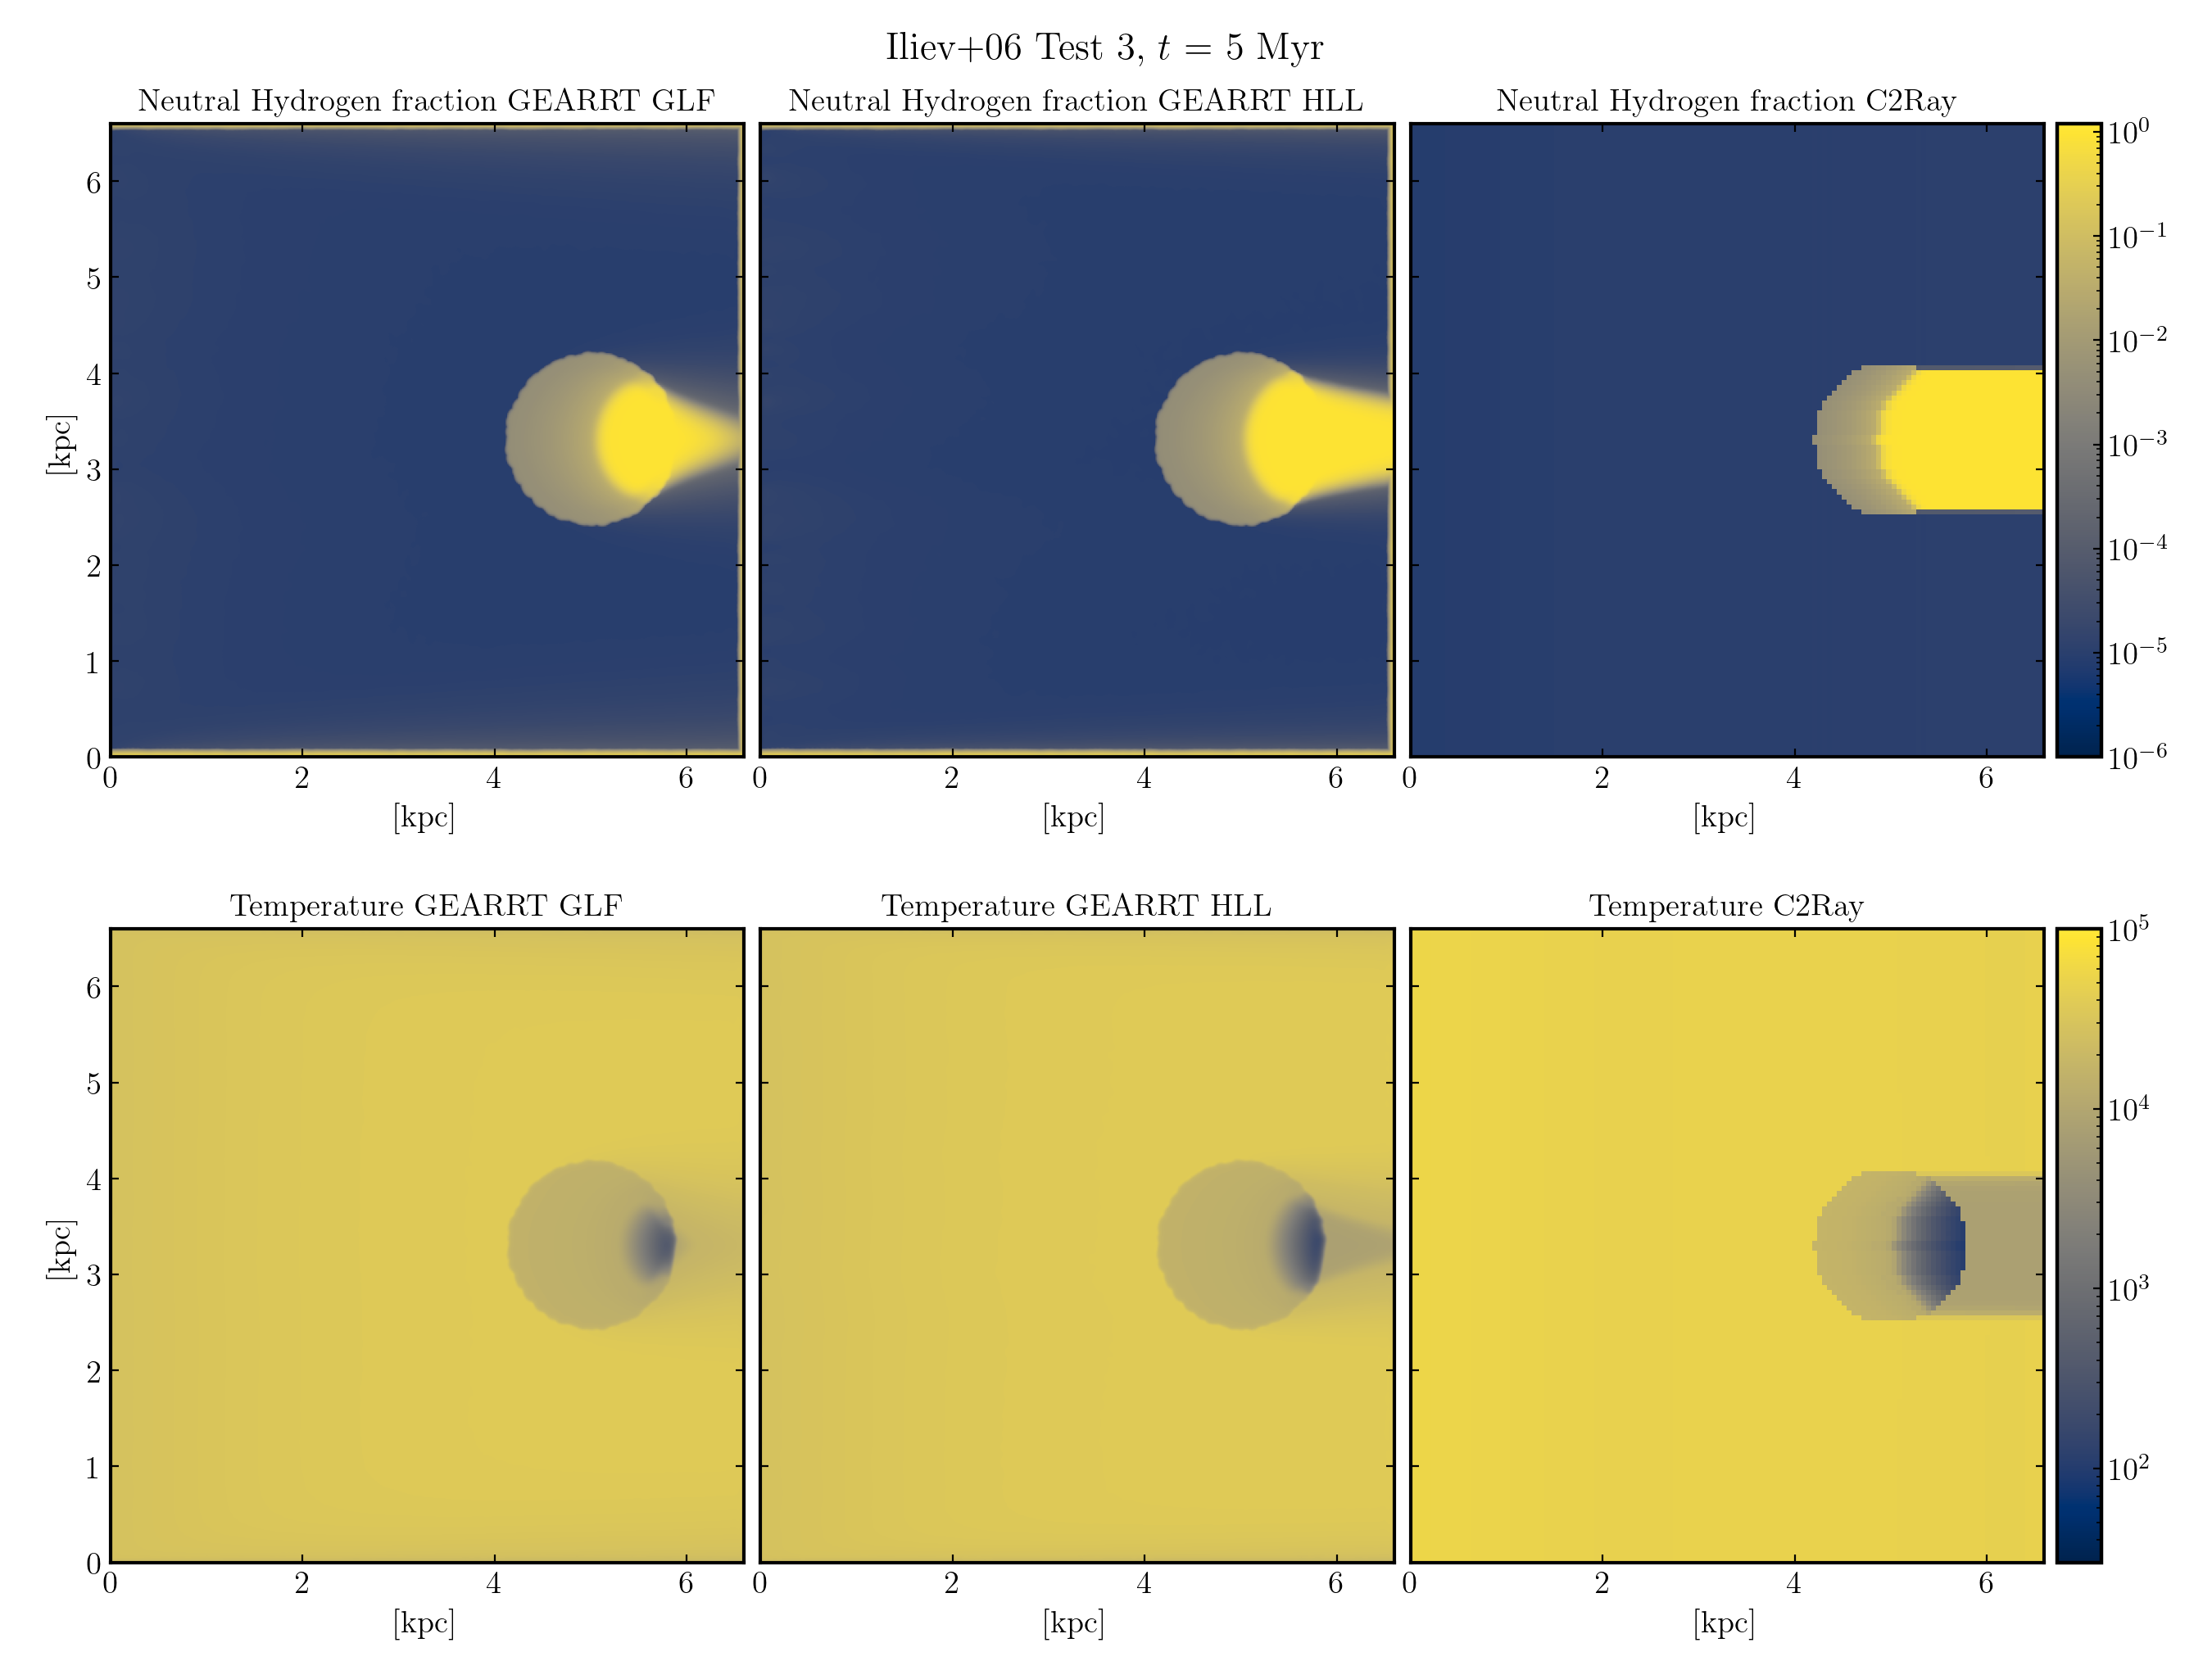
\includegraphics[width=.95\textwidth]{figures/RHD/Iliev3/comparison_128output_0005.png}\\
 \includegraphics[width=.95\textwidth]{figures/RHD/Iliev3/comparison_128output_0015.png}
 \caption{Slice along the mid-plane of Test 3 at 5 Myr (top) and 15 Myr (bottom) using both the GLF
and the HLL Riemann solver, compared with the reference solution of the \codename{C2Ray} code.
}
 \label{fig:iliev3-slices}
\end{figure}


\begin{figure}
 \centering
 \includegraphics[width=\textwidth]{figures/RHD/Iliev3/output_0001-Profiles.png}\\%
 \includegraphics[width=\textwidth]{figures/RHD/Iliev3/output_0003-Profiles.png}\\%
 \includegraphics[width=\textwidth]{figures/RHD/Iliev3/output_0015-Profiles.png}%
 \caption{
Left: Line cuts of the ionized and neutral fraction along the axis of symmetry through the center
of the clump. Right: Line cuts of the temperature along the axis of symmetry through the center of
the clump. Results are shown at times $t=$ 1, 3, and 15 Myr for \GEARRT using the HLL and the GFL
Riemann solver, for \codename{C2Ray}, and for other references.
 }
\label{fig:iliev3-profiles}
\end{figure}



\begin{figure}
 \centering
\includegraphics[
width=.85\textwidth
]{figures/RHD/Iliev3/comparisonEqualUnequalMasses_output_0005.png} \\
\includegraphics[
width=.85\textwidth
]{figures/RHD/Iliev3/comparisonEqualUnequalMasses_output_0015.png}
 \caption{
 \small{
Slice along the mid-plane of Test 3 at 5 Myr and 15 Myr for initial conditions where
particles have equal masses, and hence a higher number of particles are placed inside the clump than
outside. This is a more adequate setup for particle simulations than setting particles with regular
distances, as is done in Figure~\ref{fig:iliev3-slices}. This simulation was however produced using a
lower resolution of $\sim 64^3$ particles. The neutral gas along the edges in the solution of
\GEARRT arise due to projection effects of the boundary particles, which form an additional layer
around the box and ``swallow'' all radiation that would escape the box. The reference solution on
the right is from the \codename{C2Ray} code.}
}
 \label{fig:iliev3-equal-mass}
\end{figure}



\begin{figure}
 \centering
 \includegraphics[width=\textwidth]{figures/RHD/Iliev3/output_0001EqualMass-Profiles.png}\\%
 \includegraphics[width=\textwidth]{figures/RHD/Iliev3/output_0003EqualMass-Profiles.png}\\%
 \includegraphics[width=\textwidth]{figures/RHD/Iliev3/output_0015EqualMass-Profiles.png}\\%
 \caption{
Left: Line cuts of the ionized and neutral fraction along the axis of symmetry through the center
of the clump. Right: Line cuts of the temperature along the axis of symmetry through the center of
the clump. Results are shown at times $t=$ 1, 3, and 15 Myr for initial conditions where particles
have equal masses, and hence a higher number of particles are placed inside the clump than outside,
using $\sim 64^3$ particles, as well as when using unequal masses, but regular distances. Using
equal particle masses, which is a more adequate choice for particle simulations, significantly
improves the self-shielding of the dense clump.
 }
\label{fig:iliev3-equal-mass-profiles}
\end{figure}




\begin{figure}
 \centering
\includegraphics[
width=.85\textwidth
]{figures/RHD/Iliev3/comparisonUniform_output_0001.png} \\
\includegraphics[
width=.85\textwidth
]{figures/RHD/Iliev3/comparisonUniform_output_0005.png}
 \caption{
Slice along the mid-plane of Test 3 at 1 Myr and 5 Myr for initial conditions where particles are
placed in a glass-like distribution (left) and on a uniform grid (middle) using the HLL Riemann
solver. The reference solution on the right is from the \codename{C2Ray} code. Particles being
placed on a uniform grid improves the formation of the shadow behind the dense clump, since the
perfectly perpendicular particle placement w.r.t. to the direction of the radiation minimizes the
diffusion in the perpendicular direction.
}
 \label{fig:iliev3-uniform}
\end{figure}






% We need higher $f_c$ so radiation reaches clump by the first snapshot.

This test examines the self-shielding of a dense gas clump and the formation of a shadow. The
simulation box has a size of $6.6$ kpc. A spherical cloud of gas with radius $r_{cloud} = 0.8$ kpc
is placed centered at $(5, 3.3, 3.3)$ kpc. The surrounding hydrogen gas has an number density of
$n_{out} = 2 \times 10^{-4}$cm$^{-3}$ and temperature $T_{out} = 8000$K. The cloud is given a
number density of $T_{cloud} = 40$K and number density of $n_{cloud} = 200 n_{out}$. A constant
flux of $F = 10^6$ photons / s / cm$^2$ following a blackbody spectrum with temperature $T_{bb} =
10^{5}$K is injected from the $x = 0$ plane of the box. I again use three photon frequency
intervals split at the photo-ionizing frequencies of hydrogen and helium, leading to the same source radiation luminosities as given in eqs.~\ref{eq:group-luminisoties-1}-\ref{eq:group-luminosities-3}.
The speed of light was reduced by a factor of 8 (compared to 100 in Test 1 and 2) so that the
radiation emitted at the $x = 0$ plane would reach the clump before the first snapshot at 1 Myr as
prescribed by IL6. The particle distribution remains glass-like; In order to achieve the correct
densities in- and outside of the clump, the particle masses were modified accordingly.

This test displays a known shortcoming of moment based radiative transfer, which is its inability
to form shadows correctly. While the clump in this test is still composed of neutral hydrogen, a
shadow should form behind it. The formation of shadows is limited because the radiation, which is
being treated similar to a fluid, can diffuse into regions where light rays wouldn't. We thus test
the two different Riemann solvers described in Section~\ref{chap:riemann-rt}: The inexpensive GLF
solver, and the HLL solver, which promises to be less diffusive than the GLF solver
\citep{ramses-rt13, gonzalezHERACLESThreedimensionalRadiation2007}.

Figure~\ref{fig:iliev3-slices} shows a slice of the mid-plane of the box at 5 Myr and at 15 Myr for
both the GLF and the HLL Riemann solver, along with a reference solution of the \codename{C2Ray}
code. The HLL solver indeed improves the formation of the shadow. Figure~\ref{fig:iliev3-profiles}
shows line cuts of the neutral hydrogen mass fraction and the temperature along the axis of symmetry
of the clump at 1, 3, and 15 Myr. The improved shadow formation with the HLL solver can be seen in
the temperature profile remaining at the initial $8000$K behind the clump, i.e. at $x/L \geq 0.9$.


The line cuts in Figure~\ref{fig:iliev3-profiles} clearly reveal a further issue with the solution
obtained by \GEARRT: The ionization front penetrates much further into the dense clump than the
reference solutions. The reason for this phenomenon lies in particle nature of \GEARRT, and the
number of neighbors used.
While mesh-based codes would typically only exchange fluxes between adjacent cells, FVPM exchange
fluxes between $\sim 40-50$ neighboring particles. If these $40-50$ neighbors were arranged on a
regular grid around the particle, this would correspond to about 2 neighboring particles on each
side, and the diffusion can propagate further compared to grid codes. The diffusivity of the method
in this case can be expected to be much worse than with a mesh-based code, and the ionization front
can propagate too fast.

However, the setup in Figure~\ref{fig:iliev3-slices} and Figures~\ref{fig:iliev3-profiles} is
sub-optimal for particle codes like \GEARRT. To mimic the prescribed test setup, particles were
distributed uniformly (in a glass-like manner), and, more importantly with regard to the currently
discussed issue, assigned different masses such that the correct densities are reproduced. A more
adequate representation would be to use particles of equal masses, and adapt their positions to
reproduce the correct densities. So in this case, much more particles would be positioned inside the
clump compared to the outside region.

The results using such a setup with the GLF solver are shown in Figure~\ref{fig:iliev3-equal-mass},
albeit with a resolution of only $\sim 64^3$ particles in total.
Figure~\ref{fig:iliev3-equal-mass-profiles} shows the line cuts of the neutral hydrogen mass
fraction and the temperature along the axis of symmetry of the clump at 1, 3, and 15 Myr, comparing
the results to the ones using unequal particle masses (but somewhat regular inter-particle
distances). The improvement in the self-shielding when using particle number densities rather than
masses to represent the dense clump is evident. The formation of the shadow however isn't improved,
and is in fact worsened, since in order to keep roughly the correct total number of particles, the
rarefied region behind the clump is now sampled through fewer particles.

A contributing factor to the inadequate shadow formation with \GEARRT is the fact that it uses
particles as the underlying discretization method. In general, the particle distribution will not be regular. The exchange of fluxes (in the hyperbolic sense) between particles not perfectly aligned with the direction the radiation propagates in will lead to radiation diffusing perpendicularly to the direction of propagation, leading to reduced shadows as seen in
Figures~\ref{fig:iliev3-slices}-\ref{fig:iliev3-equal-mass-profiles}. This can be readily verified by repeating the test using a particle configuration distributed along a uniform grid. The results of such a setup are shown in Figure~\ref{fig:iliev3-uniform}, where the shadow is indeed improved.
However, the diffusivity of the method will never be able to be fully eliminated, due to several
reasons. Firstly, there will always be neighboring particles which aren't perfectly aligned with
the direction of propagation of the radiation, even on a perfectly uniform particle grid. Secondly,
the diffusivity of the method is also due to the nature of the M1 closure, and as such can't be
fully eliminated. And finally, numerical diffusion is a necessary component of the underlying
numerical method, which for FVPM enters the equation in the form of discretization errors and flux
limiters.










%========================================================
\subsection{Iliev Test 4}\label{chap:Iliev4}
%========================================================


\begin{figure}
 \centering
 \includegraphics[width=\textwidth]{figures/RHD/Iliev4/comparisonContour_output_0002.png}
 \caption{
Slice through the mid-plane of the box of the solution to Test 4 at 0.1 Myr.
Contour lines for neutral hydrogen fractions of 0.5 (solid lines) and $10^{-5}$ (dashed lines) are
shown on the left. On the right, contour lines for temperatures of $10^4$K (dashed lines) and $4
\times 10^4$K (solid lines) are shown. The solutions of \GEARRT (orange lines), \GEARRT with an
increased speed of light by a factor of 100 (blue lines) are plotted, along with the reference
solution of the \codename{C2Ray} code (green lines).
}
 \label{fig:iliev4-0.1Myr}
\end{figure}



\begin{figure}
 \centering
 \includegraphics[width=\textwidth]{figures/RHD/Iliev4/comparisonContour_output_0008.png}
\caption{
Slice through the mid-plane of the box of the solution to Test 4 at 0.8 Myr.
Contour lines for neutral hydrogen fractions of 0.5 (solid lines) and $10^{-5}$ (dashed lines) are
shown on the left. On the right, contour lines for temperatures of $10^4$K (dashed lines) and $4
\times 10^4$K (solid lines) are shown. The solutions of \GEARRT (orange lines), \GEARRT with an
increased speed of light by a factor of 100 (blue lines) are plotted, along with the reference
solution of the \codename{C2Ray} code (green lines).
}
 \label{fig:iliev4-0.4Myr}
\end{figure}


\begin{figure}
 \centering
 \includegraphics[width=\textwidth]{figures/RHD/Iliev4/output_0001-Histogram.png}\\
 \includegraphics[width=\textwidth]{figures/RHD/Iliev4/output_0004-Histogram.png}\\
 \includegraphics[width=\textwidth]{figures/RHD/Iliev4/output_0008-Histogram.png}
\caption{
Histograms of the neutral hydrogen fraction and the temperature of the entire simulation box at
times $t = $ 0.05 Myr, 0.2 Myr, and 0.4 Myr solved with the normal speed of light, and the speed of
light increased by a factor of 100.
}
 \label{fig:iliev4-histograms}
\end{figure}




In this test, a cosmological density field extracted from a simulation is being heated and ionized
by 16 sources placed at the positions of the most massive halos, and given a luminosity
proportional to the halo mass $M$. More precisely, the luminosity is assigned assuming that each
source lives for $t_s = 3$ Myr and emits $f_\gamma = 250$ ionizing photons per atom during its
lifetime, resulting in

\begin{align}
\dot{N}_\gamma = f_\gamma \frac{\Omega_b}{\Omega_0} \frac{M}{m_p} \frac{1}{t_s}
\end{align}

where $m_p$ is the proton mass, and the cosmological density parameters $\Omega_0 = 0.27$ and
$\Omega_b = 0.043$ were used. The spectrum of the emitted radiation source is again taken to be a
blackbody spectrum with effective temperature $T_{bb} = 10^5$K. I split the spectrum into three
frequency intervals at the photo-ionizing frequencies of hydrogen and helium, as given in
eqns.~\ref{eq:group-luminisoties-1}-\ref{eq:group-luminosities-3}. The simulation was extracted on a
$128^3$ grid at high redshift $z \sim 9$ for a box size of 500 $h^{-1}$ co-moving kpc. For this test, particles are also arranged on a uniform grid, and given the appropriate mass to reproduce the density field prescribed by IL6. I again use three photon frequency intervals split at the photo-ionizing frequencies of hydrogen and helium, leading to the same source
radiation luminosities as given in eqns.~\ref{eq:group-luminisoties-1}-\ref{eq:group-luminosities-3}.

Figure~\ref{fig:iliev4-0.1Myr} shows the results of \GEARRT compared with the results of
\codename{C2Ray} results at 0.1 Myr, while Figure~\ref{fig:iliev4-0.4Myr} shows the results at 0.4
Myr. In agreement to the findings in \cite{ramses-rt13}, the ionization fronts appear to propagate
slower for \GEARRT, which is likely due to the assumption of infinite speed of light used by the
ray tracing reference code \codename{C2Ray}. Following the approach of \cite{ramses-rt13}, I also
re-run the test with the speed of light \emph{increased} by a factor of 100 to approximate the
infinite speed of light for a comparison with the reference solution of \codename{C2Ray}, the
results of which are also shown in Figure~\ref{fig:iliev4-0.1Myr} and \ref{fig:iliev4-0.4Myr}.

Especially at the early times like in Figure~\ref{fig:iliev4-0.1Myr} increasing the speed of light
by a factor of 100 matches the results of \codename{C2Ray} quite well. \codename{C2Ray} however
develops more distinct features in the ionization front, which is likely due to the diffusivity of
the FVPM and the M1 closure's difficulties to capture shadows.

Figure~\ref{fig:iliev4-histograms} shows histograms of the neutral hydrogen fraction and the gas
temperature at 0.05 Myr, 0.2 Myr, and at 0.4 Myr. They confirm the previous findings: Increasing
the speed of light by a factor of 100 leads to results very similar to the reference solutions, and
nearly identical histograms of neutral hydrogen mass fractions at early times. The peak
of the temperatures however vary between \GEARRT and reference solutions due to the individual
treatment of multi-frequency and the resulting differences in the treatment of spectral hardening.
Nonetheless, the solution obtained with \GEARRT agrees fairly well with reference solutions.













%========================================================
\section{Radiation Hydrodynamics}\label{chap:IL9}
%========================================================

This section tests the radiative transfer and the thermochemistry following the standard tests set
by the comparison paper \cite{ilievCosmologicalRadiativeTransfer2009} (hereafter IL9). These tests
now involve hydrodynamics in addition to the radiative transfer and thermochemistry.
The reference solutions shown in this section are the solutions of the codes which participated in
the comparison project, whose features are summarized in Table 1 of IL9. Most of these codes, namely
\codename{C2Ray+Capreole} \citep{mellema2RayNewMethod2006, mellemaDynamicalIiRegion2006},
\codename{C2Ray+TVD} \citep{mellema2RayNewMethod2006, tracMovingFrameAlgorithm2004},
\codename{HART} \citep{kravtsovAdaptiveRefinementTree1997,
kravtsovConstrainedSimulationsReal2002,gnedinModelingMolecularHydrogen2009},
\codename{Zeus-MP} \citep{whalenMultistepAlgorithmRadiation2006},
\codename{Coral} \citep{mellemaPhotoevaporationClumpsPlanetary1998,
shapiroPhotoevaporationCosmologicalMinihaloes2004},
\codename{Flash-HC} \citep{rijkhorstHybridCharacteristics3D2006}, and
\codename{Enzo-RT} \citep{normanSimulatingCosmologicalEvolution2007a}
solved both radiative transfer and the hydrodynamics on meshes, either on uniform or adaptive ones.
\codename{RH1D} \citep{ahnDoesRadiativeFeedback2007} uses Lagrangian spherical shells instead, and
was created to solve spherically symmetric problems.
\codename{Licorice} \citep{baekSimulated21Cm2009} used a grid for radiative transfer, but SPH for
hydrodynamics, while \codename{RSPH} \citep{susaSmoothedParticleHydrodynamics2006}
used SPH for hydrodynamics and a particle-based ray-tracing method for the
radiation transport. Furthermore, with the exception of \codename{HART}, which used the variable
eddington tensor closure for the moments of the equation of radiative transfer, and
\codename{Enzo-RT}, which used the flux limited diffusion method (which only uses the zeroth
moment of the equation of radiative transfer), all other participating codes used some form of
ray-tracing to solve the radiation transport.

Unless noted otherwise, the default parameters used with \GEARRT are again to use the GLF Riemann
solver, the minmod limiter, and the ``no flux'' flux injection model. The underlying particle
distribution is glass-like. For both star and gas particles, the smoothing length is determined by
the default parameter $\eta_{res} = 1.2348$ (eq.~\ref{eq:number-of-neighbors}). This choice results
in $\sim 48$ neighbors in 3D for the cubic spline kernel, which was used for all tests without
exception. The default reduced speed of light was $\tilde{c}_r = 0.01 c$.











%========================================================
\subsection{Iliev Test 5}\label{chap:Iliev5}
%========================================================


\begin{figure}
\centering
\includegraphics[width=.8\textwidth]{figures/RHD/Iliev5/output_0001-Profiles.png}\\
\includegraphics[width=.8\textwidth]{figures/RHD/Iliev5/output_0010-Profiles.png}\\
\includegraphics[width=.8\textwidth]{figures/RHD/Iliev5/output_0020-Profiles.png}
\caption{
Spherically averaged profiles of the Test 5 problem at 10 Myr, 100 Myr, and 200 Myr. Shown are the
neutral hydrogen fraction, the ionized hydrogen fraction, the temperature, pressure, and local Mach
number of the gas. Shown are the solution of \GEARRT and reference solutions from the IL9 paper,
with \codename{C2Ray+Capreole} highlighted. The error bars are standard deviations.
}
\label{fig:iliev5}
\end{figure}



\begin{figure}
\centering
\includegraphics[width=0.7\textwidth]{figures/RHD/Iliev5/ionization_fronts.png}
\caption{
 Evolution of the I-front position and velocity over time for Test 5.
 Top: Evolution of the I-front position over time, compared to the analytical position
 Bottom: Evolution of the I-front velocity. Shown are the solution of \GEARRT and reference
 solutions from the IL9 paper, with \codename{C2Ray+Capreole} highlighted.
}
\label{fig:iliev5-Ifront}
\end{figure}




\begin{figure}
\centering
\includegraphics[width=\textwidth]{figures/RHD/Iliev5/output_0010-NoRef.png}\\
\includegraphics[width=\textwidth]{figures/RHD/Iliev5/output_0051-NoRef.png}
\caption{
Slice across the mid-plane for the Iliev Test 5 with \GEARRT at 100 Myr (top) and 500 Myr (bottom).
Shown are the neutral hydrogen fraction, the ionized hydrogen fraction, the temperature, pressure,
and local Mach number of the gas.
}
\label{fig:iliev5-slice}
\end{figure}


\begin{figure}
\centering
\includegraphics[width=\textwidth]{figures/RHD/Iliev5/compare_profiles_0020-RelativeDifferences.png}
\caption{
Spherically averaged profiles of the Test 5 problem at 200 Myr both with and without sub-cycling,
and with and without drifting particles. Shown are the neutral hydrogen fraction, the ionized
hydrogen fraction, the temperature, pressure, and local Mach number of the gas, as well as the
relative difference of the results when comparing with the run without sub-cycles.
}
\label{fig:iliev5-subcycling}
\end{figure}


This test prescribes the classical HII region expansion in an initially uniform gas. Like
in Tests 1 and 2, radiation is injected from a single source, which I place in the center of the
box to avoid needing reflective boundary conditions along the box faces, and take a box size twice
the prescribed size to a total of $30$ kpc. The gas is hydrogen only with a number density of $n =
10^{-3}$cm$^{-3}$ and initial temperature of $100$K. The resolution is $128^3$ particles, which
compared to the $128^3$ cells used in IL9 leads to half the spatial resolution due to the doubled
box size in my simulation. The spectrum of the source is taken to be a blackbody spectrum with
temperature $T_{bb} = 10^5$K, which I again split into three frequency intervals following
eqs.~\ref{eq:group-luminisoties-1}-\ref{eq:group-luminosities-3}.

Figure~\ref{fig:iliev5} shows spherically averaged profiles of the neutral hydrogen mass fraction,
the ionized hydrogen mass fraction, the gas number density, the gas temperature, pressure, and Mach
number at different times. Figure~\ref{fig:iliev5-Ifront} shows the position and velocity of
the ionization fronts over time. They agree quite well with the reference solutions.
Figure~\ref{fig:iliev5-slice} shows the slices through the mid-plane at 100 Myr and at 500 Myr, and
demonstrates that \GEARRT is able to grow nicely symmetrical Str\"omgren spheres.

As the first test which includes hydrodynamics, it offers a good opportunity to validate the
sub-cycling approach. Figure~\ref{fig:iliev5-subcycling} shows the solution to this test problem at
200 Myr performed in four different ways: The particles can either be forced to remain static, or
be used in a Lagrangian manner, which is the default behavior. Both these approaches are tested
with and without sub-cycling, and the results and their relative differences compared to the
solution with Lagrangian particles and without sub-cycling are plotted.

The sub-cycling indeed introduces a difference in regions very close to the source, which is
located at $r = 0$. This is to be expected, as in terms of spherical averaged profiles, this is a
poorly resolved region that contains only a few particles. However, comparing to reference
solutions, these differences are all in an acceptable range, and as such not deemed as an issue. A
second set of differences can be seen around the region where the shock is currently located, which
in Figure~\ref{fig:iliev5-subcycling} is located around $r/L \sim 0.5$. However, the sub-cycling
has virtually no effect there. Instead, the differences are dominated by whether the particles are
Lagrangian or static. This is to be expected, as the Lagrangian mode should allow the shock to be
better resolved, as the particles' positions will also be compressed close to the shock front.
Indeed, looking at the density profile, the two peaks around $r/L \sim 0.5$ are less pronounced
when the particles are forced to be static.








%========================================================
\subsection{Iliev Test 6}\label{chap:Iliev6}
%========================================================


\begin{figure}
\centering
\includegraphics[width=\textwidth]{figures/RHD/Iliev6/output_0003-NoRef.png}\\
\includegraphics[width=\textwidth]{figures/RHD/Iliev6/output_0010-NoRef.png}
\caption{
Slice across the mid-plane for the Iliev Test 6 with \GEARRT at 3 Myr (top) and 10 Myr (bottom).
Shown are the neutral hydrogen fraction, the ionized hydrogen fraction, the temperature, pressure,
and local Mach number of the gas. Some anisotropies develop at later times because the stronger
shock (compared to the previous tests) from the photo-heating advects too many particles away from
the inner region, leaving the central regions poorly resolved. The anisotropies are reflected in
the comparatively much bigger error bars in the profiles of these quantities in
Figure~\ref{fig:iliev6}.
}
\label{fig:iliev6-slices}
\end{figure}


\begin{figure}
\centering
\includegraphics[width=.8\textwidth]{figures/RHD/Iliev6/output_0001-Profiles.png}\\
\includegraphics[width=.8\textwidth]{figures/RHD/Iliev6/output_0010-Profiles.png}\\
\includegraphics[width=.8\textwidth]{figures/RHD/Iliev6/output_0025-Profiles.png}
\caption{
Spherically averaged profiles of the Test 6 problem at 1 Myr, 10 Myr, and 25 Myr. Shown are the
neutral hydrogen fraction, the ionized hydrogen fraction, the temperature, pressure, and local
Mach number of the gas. The error bars are standard deviations.
}
\label{fig:iliev6}
\end{figure}




\begin{figure}
\centering
\includegraphics[width=0.7\textwidth]{figures/RHD/Iliev6/ionization_fronts.png}
\caption{
 Evolution of the I-front position and velocity over time for Test 6.
 Top: Evolution of the I-front position over time, compared to the analytical position
 Bottom: Evolution of the I-front velocity.
}
\label{fig:iliev6-Ifront}
\end{figure}








This test is similar to the Test 5, but uses an inhomogeneous initial gas density of

\begin{align}
    n(r) = \begin{cases}
            n_0 & \text{ if } r \leq r_0 \\
            n_0 \frac{r_0}{r^2} & \text{ if } r \geq r_0
           \end{cases}
\end{align}

with $n_0 = 3.2$cm$^{-3}$ and $r_0 = 91.5$ pc. The box size is 0.8 kpc, which is again doubled in
my simulation. The gas has an initial temperature of $T = 100$K. The radiation source has a
blackbody spectrum with temperature $T_{bb} = 10^5$K and emits $10^{50}$ ionizing photons per
second, which is a larger emission compared to the previous tests by a factor of 20. The aim of this
test is to study the initial transition of the I-front from R-type, where the I-front propagates
much faster than the gas' response to it, to D-type, in which case the I-front propagates at about
the same velocity as the gas, and back to R-type. The initial transition from R-type to D-type
occurs during the growth of the Str\"omgren sphere, which in this test's setup occurs at $\sim
70$pc, i.e. inside the core with a flat density profile. The acceleration back to an R-type I-front
occurs due to the decreasing density after the I-front has reached the region of the density profile
with the steep gradient.





Figure~\ref{fig:iliev6-slices} shows slices through the mid-plane of the box of the solution at 1
Myr, 10 Myr, and 25 Myr. The neutral hydrogen fraction, the ionized hydrogen fraction, the
temperature, pressure, and local Mach number of the gas are shown. In this test, \GEARRT was unable
to maintain a perfectly symmetrical spherical expansion of the I-front at later times, which can be
seen particularly well in the slice at 25 Myr for the ionized hydrogen mass fraction and the mach
number. Figure~\ref{fig:iliev6} shows the spherically averaged profiles of the same quantities and
at the same times as Figure~\ref{fig:iliev6-slices}. The anisotropies can be seen in the profiles in
Figure~\ref{fig:iliev6} as comparatively much larger error bars close to the ionization front,
which show the standard deviation, compared to the results from previous tests. The reason for the
anisotropies forming is that compared to the previous tests, the heating and the resulting shock in
this test was much stronger, which lead to most particles being drifted away from the central region
behind the I-front, leaving the region poorly resolved. Indeed at 25 Myr, where the I-front is at
$r/L \sim 0.75$, only about 6.8\% of the total number of particles remained within $r/L \leq 0.75$,
whereas the initial fraction of particles within the same radius was 22.1\%. The low sampling can be
seen particularly well in the noisy Mach numbers at 10 and 25 Myr. At 25 Myr, only $\sim 2500$
particles, or 0.1\% of the total number of particles, remained within the region $r/L \leq 0.4$,
leading to the noisy results. Aside from that, the results of \GEARRT once again agree fairly well
with the reference solutions. This is also the case for the positions and velocities of the
ionization front over time, which are shown in Figure~\ref{fig:iliev6-Ifront}.











%========================================================
\subsection{Iliev Test 7}\label{chap:Iliev7}
%========================================================


\begin{figure}
\centering
\includegraphics[width=.75\textwidth]{figures/RHD/Iliev7/output_0003-GLF.png}\\
\includegraphics[width=.75\textwidth]{figures/RHD/Iliev7/output_0010-GLF.png}\\
\includegraphics[width=.75\textwidth]{figures/RHD/Iliev7/output_0025-GLF.png}
\caption{
Slices through the midplane of the box for the Iliev 7 test at 3, 10, and 25 Myr using the GLF
Riemann solver. Shown are the neutral hydrogen fraction, the ionized hydrogen fraction, the
temperature, pressure, and local Mach number of the gas.
}
\label{fig:iliev7-slices-GLF}
\end{figure}


\begin{figure}
\centering
\includegraphics[width=.75\textwidth]{figures/RHD/Iliev7/output_0003-HLL.png}\\
\includegraphics[width=.75\textwidth]{figures/RHD/Iliev7/output_0010-HLL.png}\\
\includegraphics[width=.75\textwidth]{figures/RHD/Iliev7/output_0025-HLL.png}
\caption{
Slices through the midplane of the box for the Iliev 7 test at 1, 10, and 50 Myr using the HLL
Riemann solver. Shown are the neutral hydrogen fraction, the ionized hydrogen fraction, the
temperature, pressure, and local Mach number of the gas.
}
\label{fig:iliev7-slices-HLL}
\end{figure}




\begin{figure}
\centering
\includegraphics[width=.8\textwidth]{figures/RHD/Iliev7/output_0001-Profiles.png}\\
\includegraphics[width=.8\textwidth]{figures/RHD/Iliev7/output_0010-Profiles.png}\\
\includegraphics[width=.8\textwidth]{figures/RHD/Iliev7/output_0025-Profiles.png}\\
\includegraphics[width=.8\textwidth]{figures/RHD/Iliev7/output_0050-Profiles.png}
\caption{
Line cuts along the axis of symmetry of the neutral hydrogen fraction, the ionized hydrogen
fraction, the temperature, the pressure, and the local Mach number for the Iliev 7 test at 1, 10,
25, and 50 Myr for \GEARRT using the HLL and the GLF Riemann solver, for \codename{C2Ray+Capreole},
and for other references.
}
\label{fig:iliev7-profiles}
\end{figure}







This test is set up the same way as Test 3 (Section~\ref{chap:Iliev3}): A uniform overdense clump
is placed in an otherwise uniform background density, and a plane-parallel front of radiation is
emitted from the $x = 0$ plane of the box. As in Test 3, the simulation box has a size of $6.6$ kpc.
A spherical cloud of gas with radius $r_{cloud} = 0.8$ kpc is placed centered at $(5, 3.3, 3.3)$
kpc. The surrounding hydrogen gas has an number density of $n_{out} = 2 \times 10^{-4}$cm$^{-3}$ and
temperature $T_{out} = 8000$K. The cloud is given a number density of $T_{cloud} = 40$K and number
density of $n_{cloud} = 200 n_{out}$. A constant flux of $F = 10^6$ photons / s / cm$^2$ following a
blackbody spectrum with temperature $T_{bb} = 10^{5}$K is injected from the $x = 0$ plane of the
box. The reduced speed of light used was $\tilde{c}_r = 0.125 c$ so that the incoming radiation can
reach the clump before the first required snapshot at 1 Myr.

In contrast to test 3, this test allows for the evolution of the hydrodynamics. As a consequence,
the initially dense cold clump is slowly evaporated due to the incoming radiation. As was done in
Test 3, I present results for \GEARRT using both the HLL and the GLF Riemann solvers.
Figure~\ref{fig:iliev7-slices-GLF} shows slices through the mid-plane of the box at 3, 10, and 25
Myr using the GLF solver, while Figure~\ref{fig:iliev7-slices-HLL} shows the same for the HLL
solver. A more quantitative comparison is shown in Figure~\ref{fig:iliev7-profiles}, where a line
cut along the axis of symmetry of the neutral hydrogen mass fraction, the ionized hydrogen mass
fraction, the hydrogen number density, the gas temperature, pressure, and the Mach number are shown
and compared to reference solutions at 1 Myr, 10 Myr, 25 Myr, and 50 Myr. Just as was found in Test
3, the moment based method which \GEARRT uses fails to produce sharp shadows and the region behind
the clump ($r/L \gtrsim 0.9$ at 1 Myr) heats up and ionizes, where reference solutions find the
background gas to be still in the initial state. Again the HLL solver is confirmed to perform better
at maintaining the direction of the radiation, and in providing less diffusive results in that
region. As for the hydrodynamics, the results of \GEARRT largely agree with the reference solutions.
\GEARRT finds somewhat broader peaks in the Mach number profiles at early times, but with smaller
maximal values, and can be attributed to both the more diffusive nature of the FVPM and the moment
based RT method used. The broadening on the gas velocities results in the front of the cloud
material being transported towards $r/L = 0$ a bit faster than for the reference solutions, as can
be seen in the profiles of later times. Aside from that, \GEARRT is shown to perform reasonably well
again.

















%=======================================================================
\section{Sub-Cycling Performance}\label{chap:subcycling-results}
%=======================================================================


To demonstrate the benefits of the sub-cycling scheme, the same setup as the Iliev 5 test
(Section~\ref{chap:Iliev5}) is used and evolved to 10 Myrs with varying numbers of sub-cycles.
However, instead of a gas consisting only of hydrogen, a gas composed of  75\% hydrogen and 25\%
helium by mass fractions is used. Figure~\ref{fig:subcycling-gas} shows the results of the gas mass
fractions and gas temperatures for different numbers of sub-cycles. The differences are small, and
mainly situated in the poorly resolved region close to the radiation source at $r = 0$, where the
influence of delayed particle drifts due to an increased number of sub-cycles is most influential.

Figure~\ref{fig:subcycling-speedup} shows the time-to-solution for an increasing number of
sub-cycles used compared to the case without sub-cycling. The initially steep decrease of the
required time to complete the simulation decreases and eventually nearly plateaus for 128 sub-cycles
at a time-to-solution reduction of about 50\% compared to a run without sub-cycling. The eventual
plateau is to be expected, as the sub-cycling's purpose is to allow us to omit work that may not be
strictly necessary. However, there will always be a minimal amount of work that needs to be done. In
particular, the total amount of RT time steps remains constant in all simulations regardless of how
many sub-cycles were used; Only the additional amount of hydrodynamics steps is decreased, which
can't be decreased endlessly. Eventually the minimal amount of required hydrodynamics updates will
be reached, and no further time gains will be possible by means of sub-cycling. However, more
relative improvements, i.e. relative reductions of the time-to-solution compared to a run without
sub-cycling, are expected when more physics are involved. For example,
Figure~\ref{fig:subcycling-speedup-gravity} shows the reduction in time-to-solution with increasing
numbers of sub-cycles for the same test as before, but with gravity included. Using 128 sub-cycles,
\GEARRT was able to reduce the time-to-solution by over 90\%.






\begin{figure}
    \centering
    \includegraphics[width=\textwidth]{figures/RHD/subcycling/output_HHe_0008-nsubcycles.png}
    \caption{
The gas mass fractions and temperature of the Iliev5 test (Section~\ref{chap:Iliev5}) for a gas
composed of 75\% hydrogen and 25\% helium by mass at 10 Myr when different number of sub-cycles
are used.
    }
    \label{fig:subcycling-gas}
\end{figure}




\begin{figure}
    \centering
    \includegraphics[width=.6\textwidth]{figures/RHD/subcycling/subcycles-speedup-stromgren.png}
    \caption{
The time-to-solution for varying numbers of sub-cycles compared to a simulation run without
sub-cycling.
The problem being solved is to evolve the Iliev5 test (Section~\ref{chap:Iliev5}) for a gas
composed of 75\% hydrogen and 25\% helium by mass to 10 Myr.
Note that this is not a scaling plot: The number of processors used is always the same.
    }
    \label{fig:subcycling-speedup}
\end{figure}




\begin{figure}
    \centering
\includegraphics[width=.6\textwidth]{figures/RHD/subcycling/subcycles-speedup-stromgren-gravity.png}
    \caption{
Same as Figure~\ref{fig:subcycling-speedup}, but with self-gravity included. Note that this is not a
scaling plot: The number of processors used is always the same.
    }
    \label{fig:subcycling-speedup-gravity}
\end{figure}


